% $Id: $
\documentclass[a4paper,11pt]{report}
\usepackage{a4wide}
\usepackage{tikz}
\usepackage{lscape}
\usepackage{tabularx}
\usepackage{ltablex}
\usetikzlibrary{arrows}
\usepackage[nottoc]{tocbibind}
\usepackage[titletoc]{appendix}
\usepackage{mathrsfs}
\usepackage{enumerate}
\usepackage{mcode}
\usepackage{algorithm2e}
\usepackage{mathtools}
\usepackage{amsmath,amsthm,amssymb}
\usepackage{amsfonts}
% The following makes latex use nicer postscript fonts.
\usepackage{times}
\usepackage{subcaption}
\usepackage[english]{babel}
\usepackage{tikz}
%\usepackage[colorlinks,urlcolor=blue,linkcolor=blue]{hyperref}
\pagestyle{headings}
\newcommand{\upuparrow}{\mathrel{\reflectbox{\rotatebox[origin=c]{90}{$\twoheadrightarrow$}}}}
\newcommand{\downdownarrow}{\mathrel{\reflectbox{\rotatebox[origin=c]{90}{$\twoheadleftarrow$}}}}
\usepackage{vubtitlepage}
\usepackage{lmodern}
\usepackage{graphicx}
\usepackage{natbib}
\usepackage{makeidx}
\makeindex
\usepackage[geometry]{ifsym}
%\usepackage[font=small,format=plain,labelfont=bf,up,textfont=it,up]{caption}
\renewcommand{\thefigure}{\thesection.\arabic{figure}}
\author{Filip Moons}
\title{Tiny Compiler}
%\theoremstyle{definition}
\newtheorem{theorem}{Theorem}[section]
\newtheorem{lemma}[theorem]{Lemma}
\newtheorem{proposition}[theorem]{Proposition}
\newtheorem{conjecture}{Conjecture}
\newtheorem{example}[theorem]{Example}
\let\oldexample\example
\renewcommand{\example}{\oldexample\normalfont}
\newtheorem{property}[theorem]{Property}
\newtheorem{definition}[theorem]{Definition}
\newtheorem{corollary}[theorem]{Corollary}
\newtheorem{remark}[theorem]{Remark}
\newtheorem{examples}[theorem]{Examples}
\newtheorem{remarks}[theorem]{Remarks}
\newtheorem{notation}[theorem]{Notation}

\setcounter{tocdepth}{5}
\newcommand{\maxnorm}[1]{{\left\vert\kern-0.25ex\left\vert\kern-0.25ex\left\vert #1 
    \right\vert\kern-0.25ex\right\vert\kern-0.25ex\right\vert}}
\newcommand{\N}{{\mathbb N}}
\newcommand{\Z}{{\mathbb Z}}
\newcommand{\Q}{{\mathbb Q}}
\newcommand{\R}{{\mathbb R}}
\newcommand{\C}{{\mathbb C}}
\newcommand{\HQ}{{\mathbb H}}
\renewcommand{\P}{{\mathbb P}}
\newcommand{\E}{{\mathbb E}}
\newcommand{\cost}{\text{cost}}
\newcommand{\Nash}{\text{Nash}}
\newcommand{\nash}{\text{nash}}
\newcommand{\opt}{\text{opt}}
\newcommand{\LFP}{\text{LFP}}
\renewcommand{\int}{\text{int}}
\newcommand{\graf}{\mathscr{G}}
\newcommand{\grafeen}{\mathscr{H}}
\newcommand{\hgraf}{\mathcal{G}}
\usepackage{eufrak}
\newcommand{\hgrafeen}{\mathcal{H}}
\newcommand{\vect}{\operatorname{vec}}
\newcommand{\tol}{\text{TOL}}

%\newenvironment{proof}{\noindent{\bf Bewijs.}}{{\hfill $ \ Box $}\vskip 4mm}

\promotortitle{Promotor}
\promotor{Prof. Dr. P. Cara}
\advisors{}
\author{Filip Moons}
\title{Similarity on Graphs and Hypergraphs}
\advisortitle{}
\date{MEI 2006}
\faculty{Faculty of Science}
\advisortitle{}
\department{Master of Science in Mathematics - profile: Education}
\reason{Graduation thesis submitted in partial fulfillment of the requirements
for\\ the degree of Master of Science in Mathematics - profile: Education}

\date{August 2015}


\begin{document}
% Then english TitlePage
\maketitlepage
\chapter*{Acknowledgements}
First of all, I would like to thank my promotor, Philippe Cara for his incredible attention to detail, 
for the patience he had with me and the many reminders to continue and to work 
hard. He also showed me the way to this beautiful topic for a Master thesis. Besides his role as 
promotor, I will never forget him as professor of the Linear Algebra course in 
the very first term of the BSc in Mathematics, that without any doubt was the 
most memorable course during my college years: the hard study and the stress I 
had before entering the exam room are memories that I still will be telling in my 
old days.

Secondly, I would like to thank Roger Van Nieuwenhuyze, my math lecturer during 
the teacher training I followed for one year at the Hogeschool-Universiteit Brussel. Without his encouragements, I would never have dared to leave
and study Mathematics at university level. 

I also thank all professors and teaching assistants who taught me a 
lot during the past five years. A special thanks goes to Reen Tallon, who 
always managed to overcome any administrative burden caused by the combination 
of study programs.

Last but not least, I want to thank my parents for their angry looks when they 
felt I did not study enough, it certainly kept me on track. Also my partner Sacha, my classmates, my friends from university and the Classical Liberal Student  
Union made my college years unforgettable for the rest of my life.


 
\chapter*{Abstract}
This thesis is about similarity on graphs and hypergraphs. In the first chapter, 
we give an overview of all the preliminary knowledge needed to understand 
everything in the following chapters. All the methods of similarity we will 
discuss, are eventually solving an eigenvalue problem. So it is no surprise we 
prove the Perron-Frobenius theorem and introduce the power method in the first 
chapter, the power method is a numerical algorithm to calculate the largest 
eigenvalue and a corresponding eigenvector.

In chapter 2, we give a complete overview of the research done on similarity of 
graphs. The notion of similarity originated from the HITS algorithm: this 
algorithm was developed in the late nineties to sort results of a search 
engine in a meaningful way. The algorithm uses the hyperlink structure of a set 
of webpages to assign to each webpage in the set a score in how well they are in referring to other pages
in the set (the \emph{hub}-score)  and it assigns to each webpage a score in how 
authoritative they are compared to the other sites in the set (the 
\emph{authority}-score). So you get two groups in the set of webpages: some pages are good hubs, others are good
authorities. Obviously, this dichotomy is strongly related: pages that are good 
hubs will contain a lot of links to authoritative pages, and, conversely, pages 
are good authorities when they have a lot of incoming links of good hubs. This 
algorithm was very innovative at the time, because back then,  search engine results where 
sorted based only on the number of incoming links or on the number 
occurences of the search query.

The HITS algorithm is generalized in 2004 to a notion of similarity between 
graphs. A set containing hyperlinked web pages, can indeed be seen as a graph. 
This generalization will lead to a method where we can compare two graphs by putting a similarity score
between every node of the first graph and every node of the second graph. This similarity score 
indicates how similar these nodes are: two nodes will have a high similarity 
score when their adjacent nodes will also have a high similarity score. 

Once this node similarity is introduced on graphs, we extend this notion to a 
similarity method that also returns a similarity score between the edges of two 
graphs. We will also discuss a similarity method that deals with colored 
graphs. With all these methods, we have a complete overview of the most recent 
studies about graph similarity. It is remarkable that the convergence of 
the resulting algorithm of all these methods can be proved with the same 
convergence theorem (Theorem 2.2.10.). Every solution is in fact also just an eigenvalue problem: 
every extension is a variant of the power method to calculate eigenvectors.

An important remark is that all the methods return slightly different results. 
At the moment, `the' similarity score between two vertices of a graph doesn't 
exists, simply because it depends on the method you are using: in some cases the 
results are equal (up to a constant), in other cases the results are 
different because slightly different criteria are used in the calculation. In 
that case, we can explicitly derive the difference.
Still, it is not that worse: it is important to remember that the similarity 
scores are mainly interesting when compared to other similarity scores within a graph and with one method. From that point of view,
every method give the same ranking. This is also justified by the applications: all 
of them are using similarity scores in comparison to other similarity scores. 

In the last chapter, we discover a new field: we try to transfer the concept of similarity to the more
general structure of hypergraphs. We end this chapter with a reflection on the results of the previous chapter:
when we try to develop a method for similarity on hypergraphs, which conditions must be fulfilled? Are these conditions
also met by the graph similarity methods of the first chapter? At first, we take a look at the graph 
representations of hypergraphs and we try to get a good method of similarity by 
using them. It will be clear that the incidence graph of a 
hypergraph returns the best results when used for similarity. After that, we 
also try to develop a method based on the incidence matrix. This method also fulfills all conditions. We conclude the 
thesis by proving that both methods are equal up to a constant.



\chapter*{Samenvatting}
Deze thesis bespreekt similariteit op graffen en hypergraffen. In het eerste 
hoofdstuk geven we een overzicht van alle voorkennis die nodig is om deze thesis 
te doorgronden. Bijna alle methodes die in deze thesis besproken worden, komen 
uiteindelijk neer op het oplossen van een eigenwaardeprobleem: het is dan ook 
niet verwonderlijk dat we de Perron-Frobeniusstelling bewijzen en de methode van 
de machten invoeren om eigenvectoren numeriek te berekenen.


De notie van 
similariteit op graffen, ingevoerd in hoofdstuk 2, vindt zijn oorsprong in het HITS-algoritme: dit algoritme 
werd eind jaren negentig ontdekt om zoekresultaten van een internetzoekmachine op een betekenisvolle manier 
te sorteren. Het algoritme onderzoekt de relaties tussen de hyperlinks van een verzameling webpagina's: sommige webpagina's worden 
bestempeld als goede doorverwijzers, andere webpagina's worden dan weer als een gezaghebbende bron beschouwd voor de zoekterm. 
Uiteraard is deze tweedeling sterk verwant: pagina's die goede doorverwijzers 
zijn zullen veel links naar pagina's bevatten die als een gezaghebbende bron 
gezien worden en, omgekeerd, zullen pagina's als gezaghebbende bron worden 
beschouwd als ze veel inkomende links krijgen van goede doorverwijzers. Dit 
algoritme was erg vernieuwend in die tijd, vermits tot dan toe zoekresultaten 
enkel gesorteerd werden op het aantal inkomende links (zonder daarbij de bronpagina na te gaan) 
of het aantal keren dat de zoekterm op de pagina voorkwam.

Deze methode werd rond 2004 veralgemeend naar een notie van similariteit tussen 
graffen. Een verzameling webpagina's die onderling gelinkt zijn zoals die in het HITS-algoritme gebruikt worden,
kan immers beschouwd worden als een graf. Deze veralgemening leidt tot een 
methode waarbij we een soort score kunnen kleven op hoe twee toppen van twee verschillende graffen op elkaar lijken. 
Deze `similariteisscore' zal hoger zijn als de adjacente toppen van deze twee toppen 
ook gelijkaardig zijn.

Eens we similariteit op de toppen van graffen hebben ingevoerd, gaan we deze 
methode verder uitbreiden tot similariteit op toppen en bogen van graffen en tot 
similariteit tussen gekleurde graffen. We hebben zo een compleet overzicht van 
de meest recente studies over het onderwerp. Opvallend is dat de convergentie van de resulterende algoritmes van al deze uitbreidingen via 
dezelfde convergentiestelling (Stelling 2.2.10.) kunnen bewezen worden. Elke uitbreiding komt ook 
neer op het oplossen van een eigenwaardeprobleem: uiteindelijk is elke 
uitbreiding een variant op de methode van de machten om eigenvectoren te 
berekenen.

Een belangrijke opmerking is hier wel dat deze verschillende uitbreidingen lichtjes 
andere resultaten opleveren. Er bestaat niet zoiets als `de' similariteitsscore tussen twee 
toppen van twee graffen, eenvoudigweg omdat elke uitbreiding een licht verschillend resultaat zal 
opleveren: in sommige gevallen zijn de resultaten op een constante na gelijk aan 
elkaar, in andere gevallen gebruiken de variaties iets andere criteria om 
similariteit te bepalen (bv. de methode van similariteit op de toppen van graffen en similariteit op de toppen en de bogen), waardoor
de resultaten sowieso verschillend zijn. We kunnen in dat geval wel expliciet het verschil tussen de methodes uitschrijven. Belangrijk is te onthouden 
dat similariteitscores vooral in verhouding tot de andere scores interessant zijn: we kunnen 
bv. gemakkelijk bepalen welke top van de ene graf, het meest lijkt op de top van een andere 
graf simpelweg door de grootste similariteitsscore te bekijken.    Dit zal ook blijken uit het korte overzicht van toepassingen dat op 
het einde van hoofdstuk 2 is toegevoegd, ook daar wordt een
similariteitsscore enkel in verhouding tot de andere similareitsscores bekeken.

In het laatste hoofdstuk ontdekken we tot slot nieuw terrein: we proberen 
het concept van similariteit over te brengen op de meer algemene 
structuur van hypergraffen. Dat start met een uitgebreide reflectie op de resultaten van het vorige hoofdstuk:
aan welke criteria moet zo'n similariteitsmethode voor hypergraffen allemaal voldoen? Voldoen de grafmethodes van het vorige
hoofdstuk hier ook aan? Hypergraffen kunnen door verschillende 
grafrepresentaties worden voorgesteld en we proberen eerst om via deze 
weg tot een goede methode te komen. Het zal blijken dat de incidentiegrafrepresentatie van een hypergraf de beste
resultaten oplevert. Nadien proberen 
we ook een methode te ontwikkelen aan de hand van de incidentiematrix, ook deze 
methode voldoet aan alle voorwaarden. Welnu: we kunnen bewijzen dat de methode 
met de incidentiegraf en de methode met de incidentiematrix op een constante na 
dezelfde resultaten oplevert.


 

\tableofcontents
\newpage
% \pagenumbering{arabic}
\chapter{Preliminaries and notations}


In this chapter, we give an overview of all important prelimiary knowledge 
needed to understand everything in the following chapters. We start with 
introducing different matrices and next, we prove the Perron-Frobenius theorem. 
The Perron-Frobenius theorem states that a real square matrix with nonnegative entries has a unique largest real eigenvalue (i.e. with algebraic multiplicity $1$) with an eigenvector 
that has only positive entries. The theorem was proved by Oskar 
Perron (1880-1975) in 1907 for strictly positive entries and extended by 
Ferdinand Georg Frobenius (1849-1917) to irreducible matrices with nonnegative 
entries. Next, we introduce vector and matrix norms and we prove the equivalence 
of norms and the spectral radius formula. After that, we introduce the power 
method. We conclude with the introduction of graphs and hypergraphs.

\section{Some families of matrices}\index{matrix}
In this section, we first introduce different kinds of matrices. Note that all matrices in this master thesis have real entries,
unless otherwise stated. We start with permutation matrices and their uses. 
With permutation matrices, we can introduce irreducible matrices. Also nonnegative and primitive square matrices are presented. After defining 
those, we look at the Perron-Frobenius theorem. 
\subsection{Permutation matrices}
\begin{definition}\label{petmruation}\index{permutation matrix}\index{matrix!permutation matrix}
  Given a permutation $\pi$ of $n$ elements:
  $$\pi: \{1,\ldots,n\} \to \{1,\ldots,n\},$$
  with:
    $$\pi = \begin{pmatrix} 1 & 2 & \cdots & n \\ \pi(1) & \pi(2) & \cdots & \pi(n) \end{pmatrix}, $$
  the associated \textbf{permutation matrix} $P_\pi$ is the $n\times n$-matrix 
  obtained by permuting the rows of the identity matrix $I_n$ according to $\pi$. 
  So:
 $$P_\pi = \begin{pmatrix} 
\mathbf{e}^T_{\pi(1)}  \\
\mathbf{e}^T_{\pi(2)}  \\
\vdots  \\
\mathbf{e}^T_{\pi(n)}  
\end{pmatrix}.$$
 where $\mathbf{e}_{j}$ is the $j$-th column of $I_n$, the identy matrix.
 \end{definition}
\begin{example}
  The permutation matrix $P_\pi$ corresponding to the permutation  $$\pi = \begin{pmatrix} 1 & 2 & 3 & 4 \\ 1 & 4 & 2 & 3 \end{pmatrix} $$
  is:
  $$P_\pi = \begin{pmatrix} 
1 & 0 & 0 & 0  \\
0 & 0 & 0 & 1  \\
0 & 1 & 0 & 0  \\
0 & 0 & 1 & 0  
\end{pmatrix}.$$
Note that $p_{ij} = 1$ if and only if $\pi(i) = j$. 
\end{example}

\begin{property}\label{permutatie}
A permutation matrix $P$ satisfies:
  $$PP^T = I_n.$$
 
\end{property}
\begin{proof}
By direct computation, we get with $P = (p_{ij})$:
$$(PP^T)_{ij} = \sum^n_{k=1}p_{ik}p^T_{kj} = \sum^n_{k=1}p_{ik}p_{jk}$$
Assume $i \not = j$. Then for each $k$, $p_{ik}p_{jk} = 0$ since there is only
one nonzero entry in the $k$-th row and $i \not = j$, $p_{ik}$ and $p_{jk}$ 
can't be both the nonzero entry. So, $(PP^T)_{ij} = 0$ when $i \not = j$.

When $i=j$, then there exists a $k' \in \{1,\ldots,n\}$ with $p_{ik'}p_{jk'} = 1$, 
since there is only one nonzero entry in the $k$-th row, this $k'$ is unique, 
which results in $\sum^n_{k=1}p_{ik}p_{jk} = (PP^T)_{ij} = 1$.

In other words,
$$(PP^T)_{ij} = \begin{cases} 1 &\mbox{if } i = j \\ 
0 & \mbox{otherwise} \end{cases},$$
this is exactly the formula for the entries of the identity matrix.
\end{proof}

\begin{corollary}
  The transpose of a permutation matrix $P$ is its inverse:
  $$P^T = P^{-1}.$$
  This can also more easily be concluded from the fact that a permutation matrix 
  is clearly an orthogonal matrix (a real $n \times n$-matrix with orthonormal 
  entries).
\end{corollary}
\subsection{Nonnegative and primitive matrices}
\begin{definition}\label{groterkleiner}
  Let $A$ and $B$ be two real $n\times r$-matrices. Then, $A \geq B$ (respectively $A > B$) if $a_{ij} \geq b_{ij}$ 
  (respectively $a_{ij}>b_{ij}$) for all $1 \leq i \leq n, 1 \leq j\leq r$. 
\end{definition}
\begin{definition}  A real $n\times r$-matrix $A$ is \textbf{nonnegative} if $A \geq 0$, with $0$ the $n\times r$-zero matrix.
\end{definition}\index{nonnegative matrix}\index{matrix!nonnegative matrix}
\begin{definition}  A real $n\times r$-matrix $A$ is \textbf{positive} if $A > 0$, with $0$ the $n\times r$-zero matrix.
\end{definition}\index{positive matrix}\index{matrix!positive matrix}

Since column vectors are $n \times 1$-matrices, we shall use the terms 
nonnegative and positive vector throughout. 

\begin{notation}\label{modulusmatrix}
  Let $B$ be an arbitrary complex $n\times r$-matrix, then $|B|$ denotes the 
  matrix with entries $|b_{ij}|$. This is not to be confused with the 
  determinant of a square matrix $B$, which we denote by $\det(B)$.
\end{notation}\index{modulus of a matrix}\index{matrix!modulus}

\begin{definition}  A nonnegative square matrix $A$ is called \textbf{primitive} if there is a $k \in \N_0$ such that all entries of $A^k$ are positive.
 \end{definition}\index{primitive matrix}\index{matrix!primitive matrix}

\subsection{Irreducible nonnegative matrices}
In developing the Perron-Frobenius theory, we shall first establish a series of 
theorems and lemmas on nonnegative irredicuble square matrices. 
\begin{definition}\label{defreduciebel} A square matrix $A$ is called \textbf{reducible} if there is a permutation matrix $P$ such that 
 $$PAP^T = \begin{pmatrix}  B  & 0\\
 C  & D\\
\end{pmatrix} $$
where $B,$ and $D$ are square matrices, each of size at least one and $0$ is a zero matrix.
A square matrix $A$ is called \textbf{irreducible} if it is not reducible.
 \end{definition}\index{irreducible matrix}\index{matrix!irreducible matrix}\index{reducible matrix|see {irreducible matrix}}\index{matrix!reducible matrix}

It follows immediately that a $1\times1$-matrix is always irreducible by 
definition. We now show a useful property to identify a reducible matrix.
\begin{property}\label{propertyreducible}
  Let $A$ be an $n\times n$-matrix with $n\geq 2$. Consider a nonempty, proper subset $S$ of $\{1,\ldots,n\}$ with 
  $a_{ij}=0$ for $i \in S$, 
  $j \not\in S$. Then A is  reducible.
\end{property}
\begin{proof}
  Let $S=\{i_1, i_2,\ldots, i_k\}$, where we assume, without loss of generality, 
  that $i_1 < i_2 < \cdots < i_{k-1} < i_k$. Let $S^c$ be the complement of $S$, consisting of the
  ordered set of elements $j_1 < j_3 < \cdots < j_{n-k}$. Consider the permutation $\sigma$ of
  $\{1,2,\ldots,n\}$ given by
  $$\sigma = \begin{pmatrix} 1 & 2 & \ldots & k & k + 1 & k+ 2 & \ldots & n \\ 
  i_1 & i_2 & \ldots & i_k & j_1 & j_2 & \ldots & j_{n-k} \end{pmatrix} $$

$\sigma$ can be represented by the permutation matrix $P_\sigma = (p_{ij})$, 
where $p_{rs} = 1$ if $\sigma(r) = s$. We prove that
 $$PAP^T = \begin{pmatrix}  B  & 0\\
 C  & D\\
\end{pmatrix} $$

where $B$ and $D$ are square matrices and $0$ is a $k \times (n-k)$ zero matrix. 
Consider row $c$ and column $d$, where $1 \leq c \leq k$ and $k + 1 \leq d \leq
n$:
\begin{eqnarray}\label{redenering1}
(PAP^T)_{cd} = \sum_i\sum_j p_{c i}a_{ij}p_{d j}.
\end{eqnarray}
It is enough to show that each term in the summation is zero. Suppose $p_{c i} =
p_{d j} = 1$. Thus $\sigma(c) = i$ and $\sigma(d)= j.$ Since $1 \leq c \leq
k$, then $i \in \{i_1, i_2,\ldots, i_k\}$; similarly, since $k+1 \leq d \leq n$, we have $j \in 
\{j_1,j_2,\ldots,j_{n-k}\}.$ By assumption, for such a pair $i, j$, we have $a_{ij}=0$. That completes
the proof. 
\end{proof}
We know prove some equivalent definitions for a nonnegative, irreducible square 
matrix.
\begin{theorem}\label{irredubieleegenschappen}\index{irreducible matrix}\index{matrix!irreducible matrix}
  Let $A\geq 0$ be a nonnegative $n\times n$-matrix. Then the following conditions are 
  equivalent:
  \begin{enumerate}
    \item[(1)] $A$ is irreducible.
    \item[(2)] $(I + A)^{n-1} > 0$
   \item[(3)] For any pair $(i,j)$, with $1 \leq i, j \leq n$, there is a 
   positive integer $k = k(i,j) \leq n$ such that $(A^k)_{ij} > 0$.
  \end{enumerate}
\end{theorem}
\begin{proof}
  
  $(1) \Rightarrow (2)$: Let $\mathbf{x} \geq 0, \mathbf{x} \not = \mathbf{0}$ be an arbitrary vector in $\R^n$.
  If a coordinate of $\mathbf{x}$ is positive, the same coordinate is positive  in $\mathbf{x} + A\mathbf{x} = (I+A)\mathbf{x}$ 
  as well. We claim that $(I+A)\mathbf{x}$ has fewer zero coordinates than 
  $\mathbf{x}$ as long as $\mathbf{x}$ has a zero coordinate. If this claim is 
  not true, then the number of zero coordinates must be at least equal,
  this means that for each coordinate $j$ with $x_j = 0$ we would have that $x_j+ (A\mathbf{x})_j= 0$. Let $J = \{j: x_j > 0\}.$ For any $j \not \in J, r\in J$, we have 
  $(A\mathbf{x})_j = \sum_k a_{jk}x_k = 0$ and $x_r > 0$. 
  It must be that $a_{jr} = 0$. It follows from Property \ref{propertyreducible} that $A$ 
  is reducible, which is a contradiction and the claim is proved. Thus $(I+A)\mathbf{x}$ 
  has at most $n-2$ zero coordinates. Continuing in this manner we conclude that 
  $(I + A)^{n-1}\mathbf{x} > 0$. Let $\mathbf{x} = \mathbf{e}_i$, then the corresponding column of $(I+A)^{n-1}$ must be 
  positive. Thus (2) holds.
  
  $(2) \Rightarrow (3)$: We have $(I + A)^{n-1} > 0$, $A \geq 0$, so $A \not = 0$ 
  and 
  $$A(I+A)^{n-1} = \sum_{k=1}^n {n-1 \choose k-1} A^k > 0.$$
Thus for any $i, j$ at least one of the matrices $A, A^2,\ldots, A^n$ has its 
$(i,j)$-th element entry positive.

$(3) \Rightarrow (1)$: Suppose $A$ is reducible. Then for some permutation 
matrix $P$,
$$PAP^T = \begin{pmatrix}  B_1  & 0\\
 C_1  & D_1\\
\end{pmatrix} $$
where $B_1$ and $D_1$ are square matrices. Furthermore, we know from Property \ref{permutatie} that 
$PAP^TPAP^T = PA^2P^T$,
hence for some square matrices $B_2, C_2$ we have:
$$PA^2P^T = \begin{pmatrix}  B_2  & 0\\
 C_2  & D_2\\
\end{pmatrix} $$
More generally, for some matrix $C_t$ and square matrices $B_t$ and $D_t$,
$$PA^tP^T = \begin{pmatrix}  B_t  & 0\\
 C_t & D_t\\
\end{pmatrix} $$
Thus $(PA^tP^T)_{rs} = 0$ for $t = 1, 2,\ldots$ and for any $r,s$ 
corresponding to an entry of the zero submatrix in $PAP^T$.
Now, for $t = 1,\ldots,n:$
$$0 = (PA^tP^T)_{rs} = \sum_k\sum_l p_{r k}a_{kl}^{(t)}p_{l s}$$
By using the same reasoning as in \ref{redenering1}, choose $r,s$ so that $p_{r k} = p_{l s} = 1$. Then $a^{(t)}_{kl} = 0$ for all $t$,
contradicting the hypothesis. This completes the proof. 
 \end{proof}
 
 
 \begin{corollary}\index{primitive matrix}\index{matrix!primitive matrix}

   If $A$ is irreducible then $I+A$ is primitive. 
 \end{corollary}
 \begin{corollary}\index{irreducible matrix}\index{matrix!irreducible matrix}
   $A^T$ is irreducible whenever $A$ is irreducible.
 \end{corollary}
 \begin{property}\label{geenzerorij}\index{vanishing}

  No row or column of an irreducible matrix $A$ can vanish. This means that $A$ cannot have a row or a column of zeros.
   \end{property}
 \begin{proof}
   Suppose that $A$ has a zero row, then it could be permuted to
   
\begin{eqnarray*}PAP^T = \left(\begin{array}{c|c}  0 & 0 \ldots 0\\
     \hline
\begin{array}{l}
c_1  \\
\vdots \\
c_n\\   
\end{array}
 & D\\
 \end{array}\right) \end{eqnarray*}
 by some permutation matrix $P$. It follows from Definition \ref{defreduciebel} 
 that $A$ is reducible. Similarly, if $A$ has zero column, it can be permuted 
 to
   $$PAP^T = \left(\begin{array}{c|c} B & \begin{tabular}{l}
0 \\
\vdots \\
0\\   
\end{tabular}\\
\hline
    c_1  \ldots c_n   & 0\\
 \end{array}\right), $$
    again from Definition \ref{defreduciebel} we conclude that $A$ is reducible.

 \end{proof}
 
 
\newpage
 \section{Perron-Frobenius Theorem}
 We know prove the Perron-Frobenius theorem. The results of this section are 
 mainly based on the book `Elemetary Matrix Theory' of H.W. Eves 
 \cite{wngebruikt}. Although the proof of the Perron-Frobenius is very straightforward in this work, it 
 was sometimes necessary to extend the reasonings in some proofs, the books 
 \cite{horn2} and \cite{horn} were very helpful in this case.
 
 
 \subsection{Spectral radii of nonnegative matrices}
 
 \begin{definition}\index{spectral radius}\index{matrix!spectral radius}
  Let A be an $n\times n$-matrix with real entries and eigenvalues $\lambda_i$,
  $1 \leq i \leq n$. Then:
  $$\rho(A) = \max_{1 \leq i \leq n} |\lambda_i|$$
  is called the \textbf{spectral radius} of the matrix $A$.
\end{definition}

Geometrically, if all the eigenvalues $\lambda_i$ of $A$ are plotted in the 
complex plane, then $\rho(A)$ is the radius of the smallest disk $|z| \leq 
R$, with center at the origin, which includes all the eigenvalues of the matrix 
$A$.

 We now establish a series of lemmas on nonnegative irreducible square matrices. 
 These lemmas will allow us to prove the Perron-Frobenius at the end of this
 section.\\
 
 If $A \geq 0$ is an irreducible $n\times n$-matrix and $\mathbf{x}$, a vector of size $n$ with $\mathbf{0} \not = \mathbf{x} \geq 0$, let
 \begin{eqnarray}
r_\mathbf{x} = \min\left\{\frac{\sum^n_{j=1}a_{ij}x_j}{x_i}\right\}
  \end{eqnarray}
 where the minimum is taken over all $i$ for which $x_i > 0$. Clearly, $r_\mathbf{x}$ is 
 a nonnegative real number and is the supremum of all $p \geq 0$ for 
 which 
  \begin{eqnarray}\label{eenvoudigefrob}
A\mathbf{x} \geq p\mathbf{x}  \end{eqnarray}
 
  We now consider the nonnegative quantity $r$ defined by 
 \begin{eqnarray}\label{eenvoudigefrob2}\label{quantityr}
   r = \sup_{\begin{subarray}{l}\mathbf{x} \geq 0\\
    \mathbf{x}\not = \mathbf{0}\end{subarray}} \{r_\mathbf{x}\}
 \end{eqnarray}
As $r_{\mathbf{x}}$ and $r_{\alpha\mathbf{x}}$ 
have the same value for any 
scalar $\alpha > 0$, we need consider only the set $B$ of vectors $\mathbf{x} \geq 0$ 
with $||\mathbf{x}|| = 1$, and we correspondingly let $Q$ be the set of all vectors $\mathbf{y}=(I+A)^{n-1}\mathbf{x}$ 
where $\mathbf{x} \in B$. From Theorem \ref{irredubieleegenschappen} , $Q$ 
consists only of positive vectors. Multiplying both sides of the inequality $A\mathbf{x} \geq r_{\mathbf{x}}\mathbf{x}$
by $(I+A)^{n-1}$, we obtain:

$$\forall \mathbf{y} \in Q: A\mathbf{y} \geq r_{\mathbf{x}}\mathbf{y},$$
and we conclude from (\ref{eenvoudigefrob}) that $r_\mathbf{y} \geq 
r_{\mathbf{x}}$. Therefore, the quantity $r$ of (\ref{eenvoudigefrob2}) can be 
defined equivalently as:
\begin{eqnarray}\label{quantityr2}
  r = \sup_{\mathbf{y} \in Q} \{r_{\mathbf{y}}\}
\end{eqnarray}
As $B$ is a compact set (in the usual topology) of vectors, so is $Q$, and as $r_\mathbf{y}$ is a continuous 
function on $Q$, we know from the extreme value theorem that there necessarily exists a positive vector $\mathbf{z}$ for which:
\begin{eqnarray}\label{frobbrol3}
  A\mathbf{z} \geq r\mathbf{z},
 \end{eqnarray}
 and no vector $\mathbf{w} \geq 0$ exists for which $A\mathbf{w} > r\mathbf{w}$. 
\begin{definition}
  We call all nonnegative, nonzero vectors $\mathbf{z}$ satisfying 
  (\ref{frobbrol3})
  \textbf{extremal vectors} of the matrix $A$.
\end{definition}

\begin{lemma}
  If $A \geq 0$ is an irreducible $n\times n$-matrix, the quantity $r$ of (\ref{quantityr}) 
  is positive.
\end{lemma}
\begin{proof}
  If $\mathbf{x}$ is the positive vector whose coordinates are all unity, then since the matrix $A$ is irreducible, 
  we know from Property \ref{geenzerorij} that no row of $A$ can vanish, and consequently no component of $A\mathbf{x}$ 
  can vanish. Thus, $r_\mathbf{x} > 0$, proving that $r > 0$.
  \end{proof}
  
  \begin{lemma}\label{lemmafrobextremal} If $A \geq 0$ is an irreducible $n\times n$-matrix, each extremal vector $\mathbf{z}$ is a positive 
  eigenvector of $A$ with corresponding eigenvalue $r$ of (\ref{quantityr}), i.e., $A\mathbf{z} 
  = r\mathbf{z}$ and $\mathbf{z} > 0$.
  \end{lemma}
  \begin{proof}
    Let $\mathbf{z}$ be an extremal vector with $A\mathbf{z} - r \mathbf{z}= 
    \mathbf{t}$. If $\mathbf{t}\not = \mathbf{0}$, then some coordinate of $\mathbf{t}$ is 
    positive; multiplying through by the matrix $(I+A)^{n-1}$, we have:
    $$A\mathbf{w} - r\mathbf{w} > 0, \text{ with } \mathbf{w} = (I+A)^{n-1}\mathbf{z}$$
    from Theorem \ref{irredubieleegenschappen} we know that $\mathbf{w} > 0$. It 
    would then follow that $r_{\mathbf{w}} > r$, contradicting the definition of 
    $r$ in (\ref{quantityr2}). Thus $A\mathbf{z} = r\mathbf{z}$, and since 
    $\mathbf{w} > 0$ and $\mathbf{w} = (1+r)^{n-1}\mathbf{z}$, then we have $\mathbf{z} 
    > 0$, completing the proof.
  \end{proof}
  
  \begin{lemma}\label{lemma2frobvolledig}
    Let $A \geq 0$ be an irreducible $n\times n$-matrix, and let $B$ be an $n\times 
    n$- complex matrix with $|B|\leq A$. If $\beta$ is any eigenvalue of $B$, 
    then 
\begin{eqnarray}\label{lemma2frob}
|\beta| \leq r,  
\end{eqnarray}
where $r$ is the positive quantity of (\ref{quantityr}). Moreover, equality is 
valid in (\ref{lemma2frob}), i.e., $\beta = re^{i\phi}$, if and only if $|B| = 
A$, and where $B$ has the form:
\begin{eqnarray}\label{lemma2frobvormB}
B = e^{i\phi}DAD^{-1},
\end{eqnarray}
and $D$ is a diagonal matrix whose diagonal entries have modulus unity.
  \end{lemma}
  
  
  \begin{proof}
  If $\beta\mathbf{y} = B\mathbf{y}$ where $\mathbf{y} \not = \mathbf{0}$, then
  $$\beta y_i = \sum_{j=1}^n b_{ij}y_i, \text{ with } 1 \leq i \leq n.$$
  Using the hypotheses of the lemma and the notation of Definition \ref{modulusmatrix}, it follows that:
  \begin{eqnarray}
|\beta||\mathbf{y}| \leq |B||\mathbf{y}| \leq A |\mathbf{y}|,
\end{eqnarray}
which implies that $|\beta| \leq r_{|\mathbf{y}|} \leq r$, proving 
(\ref{lemma2frob}). If $|\beta| = r$, then $|\mathbf{y}|$ is an extremal vector 
of $A$. Therefore, from Lemma \ref{lemmafrobextremal}, $|\mathbf{y}|$ is a 
positive eigenvector of $A$ corresponding to the positive eigenvalue $r$. Thus,
\begin{eqnarray}\label{lemma2frobconclusion}
  r|\mathbf{y}| = |B||\mathbf{y}| = A|\mathbf{y}|,
\end{eqnarray}
and since $|\mathbf{y}| > 0$, we conclude from (\ref{lemma2frobconclusion}) and 
the hypothesis $|B| \leq A$ that 
\begin{eqnarray}\label{lemma2frobBeqA}  |B| = A
  \end{eqnarray}
For the vector $\mathbf{y}$, where $|\mathbf{y}| > 0$, let
$$D = \text{diag}\left\{\frac{y_1}{|y_1|}, \ldots, \frac{y_n}{|y_n|}\right\}.$$
It is clear that the diagonal entries of $D$ have modulus unity, and
\begin{eqnarray}
  \mathbf{y} = D|\mathbf{y}|.
    \end{eqnarray}
Setting $\beta = re^{i\phi}$, then $B\mathbf{y} = \beta\mathbf{y}$ can be 
written as:
\begin{eqnarray}\label{lemma2frobC}
  C|\mathbf{y}| = r|\mathbf{y}|,
\end{eqnarray}
where
\begin{eqnarray}\label{lemma2frobdefC}
  C = e^{-i\phi}D^{-1}BD.
\end{eqnarray}
From (\ref{lemma2frobconclusion}) and (\ref{lemma2frobC}), equiting terms equal 
to $r|\mathbf{y}|$ we have
\begin{eqnarray}\label{lemma2frobequalsmatriceswithy}
 C|\mathbf{y}| = |B||\mathbf{y}| = A|\mathbf{y}|.
 \end{eqnarray}
 From the definition of the matrix $C$ in (\ref{lemma2frobdefC}), $|C| = |B|$. 
 Combining with (\ref{lemma2frobBeqA}), we have:
 \begin{eqnarray}\label{lemma2frobequalsmatrices}
 |C| = |B| = A.
 \end{eqnarray}
 Thus, from (\ref{lemma2frobequalsmatriceswithy}) we conclude that $C|\mathbf{y}| = 
 |C||\mathbf{y}|$, and as $|\mathbf{y}| > 0$, it follows that $C = |C|$ and thus $C = A$ from  
 (\ref{lemma2frobequalsmatrices}). Combining this result with 
 (\ref{lemma2frobdefC}), gives the desired result that $B = e^{i\phi}DAD^{-1}$. 
 Conversely, it is obvious that if $B$ has the form in (\ref{lemma2frobvormB}), 
 then $|B|=A$, and $B$ has an eigenvalue $\beta$ with $|\beta| = r$, which 
 completes the proof.
\end{proof}

\begin{corollary}\label{lemma2frobcorollary}
  If $A \geq 0$ is an irreducible $n\times n$-matrix, then the positive 
  eigenvalue $r$ of Lemma \ref{lemmafrobextremal} equals the spectral radius $\rho(A)$ 
  of $A$
\end{corollary}  
\begin{proof}
  Setting $B = A$ in Lemma \ref{lemma2frobvolledig} immediately gives us this
  result.
\end{proof}
 In other words, if $A \geq 0$ is an irreducible $n\times n$-matrix, its 
 spectral radius $\rho(A)$ is positive, and the intersection in the complex 
 plane of the circle $|z| = \rho(A)$ with the positive real axis is an 
 eigenvalue of $A$.
 \begin{definition}\index{principal square submatrix}\label{principalsubmatrix}
 A \textbf{principal square submatrix} of an $n\times n$-matrix A is any 
   matrix obtained by crossing out any $j$ rows and the corresponding $j$
 columns of $A$, with $1 \leq j \leq n.$ \end{definition}
 \begin{lemma}\label{froblemma4}
   If $A \geq 0$ is an irreducible $n\times n$-matrix, and $B$ is any principal 
   square submatrix of $A$, then $\rho(B) < \rho(A).$
 \end{lemma}
 \begin{proof}
   If $B$ is any principal submatrix of $A$, then there is an $n\times 
   n$-permutation matrix $P$ such that $B = A_{11}$ where
   \begin{eqnarray}
    C = \begin{pmatrix}  A_{11}  & 0\\
 0  & 0\\
\end{pmatrix};
PAP^T =  \begin{pmatrix}  A_{11}  & A_{12}\\
 A_{21}  & A_{22}\\
\end{pmatrix}
  \end{eqnarray}
Here, $A_{11}$ and $A_{22}$ are, respectively, $m\times m$ and $(n-m) \times (n-m)$ 
principal square submatrices of $PAP^T$, $1 \leq m \leq n.$ Clearly, $0\leq C \leq 
PAP^T$, and $\rho(C) = \rho(B) = \rho(A_{11})$, but as $C = |C| \not = PAP^T$, 
the conclusion follows immediately from Lemma \ref{lemma2frobvolledig} and 
Corollary \ref{lemma2frobcorollary}.
 
  \end{proof}


   The following lemma is used to prove that $\rho(A)$ is a simple 
   eigenvalue of $A$ in the Perron-Frobenius theorem. The proof uses the 
   extension of the product rule of derivation for multilinear functions 
   $M(a_1,\ldots,a_k)$. Suppose $x_1,..,x_k$ are differentiable vector functions, 
   then $M(x_1,\ldots,x_k)$ is differentiable and:
   $$\frac{\mathrm{d}}{\mathrm{d}t}M(x_1,\ldots, x_k) = M(\frac{\mathrm{d}}{\mathrm{d}t} x_1, x_2, \ldots, x_k) 
   + M(x_1, \frac{\mathrm{d}}{\mathrm{d}t} x_2, \ldots, x_k) + \ldots +  M(x_1,  x_2, \ldots,\frac{\mathrm{d}}{\mathrm{d}t} x_k) $$
   The most important application of this rule is for the derivative of the determinant:
   $$\frac{\mathrm{d}}{\mathrm{d}t}\det(x_1,\ldots, x_k) = \det(\frac{\mathrm{d}}{\mathrm{d}t} x_1, x_2, \ldots, x_k) 
   + \det(x_1, \frac{\mathrm{d}}{\mathrm{d}t} x_2, \ldots, x_k) + \ldots + \det(x_1,  x_2, \ldots,\frac{\mathrm{d}}{\mathrm{d}t} x_k) $$

 \begin{lemma}\label{maclane}

   Let $A$ be an $n \times n$-matrix over the complex numbers and let $\phi(A, \lambda) = \det(\lambda I_n - A)$
   be the characteristic polynomial of $A$. Let $B_i$ be the principal submatrix 
   of $A$ formed by deleting the $i$-th row and column of $A$ and let $\phi(B_i, \lambda)$ 
   be the characteristic polynomial of $B_i$. Then:
   $$\phi'(A, \lambda) = \frac{\mathrm{d}\phi(A, \lambda)}{\mathrm{d}\lambda}= 
   \sum_i \phi(B_i, \lambda)$$
 \end{lemma}
\begin{proof}
  The proof is immediately done by direct computation:
  
  $$\phi(A, \lambda) = \det\begin{pmatrix} 
\lambda -a_{1,1} & -a_{1,2}  & \ldots & -a_{1,n}   \\
-a_{2,1}  & \lambda - a_{2,2} & \ldots & -a_{2,n}   \\
\vdots & \vdots & \ddots & \vdots  \\
- a_{n,1}  & -a_{n,2} & \ldots & \lambda - a_{n,n}  
\end{pmatrix}.$$
Using the extension of the product rule of derivation for multilinear functions
\begin{eqnarray*}
  \phi'(A, \lambda) = \det\begin{pmatrix} 
1 & 0  & \ldots & 0    \\
-a_{2,1}  & \lambda - a_{2,2} & \ldots & -a_{2,n}   \\
\vdots & \vdots & \ddots & \vdots  \\
- a_{n,1}  & -a_{n,2} & \ldots & \lambda - a_{n,n}  
\end{pmatrix} + 
\det\begin{pmatrix} 
\lambda -a_{1,1} & -a_{1,2}  & \ldots & -a_{1,n}   \\
0  & 1 & \ldots &  0   \\
\vdots & \vdots & \ddots & \vdots  \\
- a_{n,1}  & -a_{n,2} & \ldots & \lambda - a_{n,n}  
\end{pmatrix} + \ldots \\
+ \det\begin{pmatrix} 
\lambda -a_{1,1} & -a_{1,2}  & \ldots & -a_{1,n}   \\
-a_{2,1}  & \lambda - a_{2,2} & \ldots & -a_{2,n}   \\
\vdots & \vdots & \ddots & \vdots  \\
0  & 0 & \ldots & 1
\end{pmatrix} = \sum_i \phi(B_i, \lambda).
\end{eqnarray*}
\end{proof}
\subsection{Proof}
We now collect the above results into the following main theorem: we finally 
arrived at the Perron-Frobenius Theorem:
\begin{theorem}(\textbf{Perron-Frobenius theorem})\label{frobtheorem}\index{Perron-Frobenius}

  Let $A \geq 0$ be an irreducible $n\times n$-matrix. Then,
  \begin{enumerate}
    \item $A$ has a positive real eigenvalue equal to its spectral radius.
    \item To $\rho(A)$ there corresponds an eigenvector $\mathbf{x} > 0$.
    \item $\rho(A)$ increases when any entry of $A$ increases.
    \item $\rho(A)$ is a simple eigenvalue of $A$.
    \item If $A\mathbf{x} = \rho(A)\mathbf{x}$ where $\mathbf{x} > 0$ and $\mathbf{x}$ 
    is a normalized vector, then $\mathbf{x}$ is unique.
    
  \end{enumerate}
  \end{theorem}
 \begin{proof}
  (1) and (2) follow immediately from Lemma \ref{lemmafrobextremal} and 
   Corollary \ref{lemma2frobcorollary}. 
   
  (3) Suppose we increase 
   some entry of the matrix $A$, giving us a new irreducible matrix $\tilde{A}$ 
   where $\tilde{A} \geq A$ and  $\tilde{A} \not = A$. Applying Lemma 
   \ref{lemma2frobvolledig}, we conclude that $\rho(\tilde{A}) > \rho(A).$ 
   
   (4) $\rho(A)$ is a simple eigenvalue of $A$, i.e., $\rho(A)$ is a zero of multiplicity one of the characteristic polynomial
   $\phi(\lambda) = \det(\lambda I_n - A)$, we make use of Lemma \ref{maclane} by using the fact that $\phi'(\lambda)$ is the sum of the
   determinants of the principal $(n-1)\times(n-1)$ submatrices of $\lambda I - A$. If $A_i$ is any principal submatrix of
   $A$, then from Lemma \ref{froblemma4}, $\det(\lambda I - A_i)$ (with $I$ the identity matrix with the same size as the principal submatrix $A_i$) cannot vanish 
   for any $\lambda \geq \rho(A)$. From this it follows that:
   $$\det(\rho(A)I - A_i) > 0,$$
   and thus
   $$\phi'(\rho(A)) > 0.$$
   Consequently, $\rho(A)$ cannot be z zero of $\phi(\lambda)$ of multiplicity 
   greater than one and thus $\rho(A)$ is a simple eigenvalue of $A$. 
   
  (5) If $A\mathbf{x} = \rho(A)\mathbf{x}$ where $\mathbf{x} > 0$ 
   and $||\mathbf{x}|| = 1$ ($\|\cdot \|$ denotes the standard Euclidean norm), we cannot find 
   another eigenvector $\mathbf{y} \not = s\mathbf{x}$, with $s$ a scalar, of $A$ 
   with $A\mathbf{y} = \rho(A)\mathbf{y}$, so that the eigenvector $\mathbf{x}$ 
   , meaning that the normalized eigenvector $\mathbf{x}$ is uniquely 
   determined.
       \end{proof}

   
   With the previous proof in mind, the following definition comes not unexpected:
   
   \begin{definition}\label{perronroot}\index{Perron root}\index{Perron vector}
     If a matrix $A$ has an eigenvalue equal to the spectral radius $\rho(A)$, this eigenvalue
     is called the \textbf{Perron root}, the corresponding eigenvector $\mathbf{x}$ such that:
     $$A\mathbf{x} = \rho(A)\mathbf{x} \quad \text{and} \quad \|\mathbf{x}\|_1 = 1$$ is called 
     the \textbf{Perron vector}.
   \end{definition}

\begin{corollary}
  Being a strictly positve square matrix ($A >0$) is a sufficient condition to apply the Perron-Frobenius Theorem.
\end{corollary}
\begin{proof}
  This follows immediately from Theorem \ref{irredubieleegenschappen}: a 
  positive square matrix is always irreducible.
\end{proof}  

\subsection{Example}
To check wether a matrix with nonnegative entries is primitive, irreducible or 
neither, we just have to replace all nonzero entries by 1 since this does not 
affect the classification. The matrix
$$\begin{pmatrix}1 & 1\\
1 & 1 \\
\end{pmatrix}$$
is strictly positive and thus primitive. The matrices
$$\begin{pmatrix}1 & 0\\
1 & 1 \\
\end{pmatrix}\text{\;\;\; and \;\;\,} 
\begin{pmatrix}
1 & 1\\
0 & 1 \\
\end{pmatrix}$$
both have 1 as a double eigenvalue hence cannot be irreducible.
The matrix $\begin{pmatrix}
1 & 1\\
1 & 0 \\
\end{pmatrix}$ satisfies:
$$\begin{pmatrix}
1 & 1\\
1 & 0 \\
\end{pmatrix}^2 = \begin{pmatrix}
2 & 1\\
1 & 1 \\
\end{pmatrix}$$
and hence is primitive. The same goes for $$\begin{pmatrix}
0 & 1\\
1 & 1 \\
\end{pmatrix},$$ this matrix is irreducible but not primitive. Its 
eigenvalues are $1$ and $-1$.
\newpage
\section{Norms}
If one has several vectors in $\R^n$ or several matrices in $\R^{n\times m}$, 
how do we measure that some of them are `large' and some of them are `small'? 
One way to answer this question is to study norms, which are basically functions 
that assign a positive `size' to a vector in a vector space. The norms that we define 
in this master thesis are limited to $\R^n$ and $\R^{n\times m}$ and we call 
them respectively \emph{vector norms} (norms on $\R^n$) and \emph{matrix norms} (norms on $\R^{n\times 
m}$). This section is mainly based on chapter 2 from \cite{golub} and chapter 5 
form \cite{horn}.

\subsection{Vector norms}
\begin{definition}\label{vectornorms}\index{vector norm}
  A \textbf{vector norm} on $\R^n$ is a function $\|\cdot\|: \R^n \to \R$ with 
  the following properties:
  \begin{enumerate}
 \item $\|\mathbf{x}\| \geq 0$, for all $\mathbf{x} \in \R^n$ with equality if 
 and only if $\mathbf{x} = \mathbf{0}$.
 \item $\|\mathbf{x} + \mathbf{y}\| \leq \|\mathbf{x}\| + \|\mathbf{y}\|$ for 
 all $\mathbf{x},\mathbf{y} \in \R^n$.
 \item $\|\alpha \mathbf{x}\| = |\alpha|\|\mathbf{x}\|$ for all $\alpha \in \R$, $\mathbf{x} \in 
 \R^n$.
  \end{enumerate}
\end{definition}



We now give some well known vector norms:
\subsubsection{$p$-norms}\index{$p$-norm}\index{vector norm!$p$-norm}\index{H\"{o}lder norm|see{$p$-norm}}
\begin{definition}\label{holderdebolder}
  The \textit{H\"{o}lder} or  \emph{p-norms} are defined by:
  $$\|\mathbf{x}\|_p = (|x_1|^p+\cdots + |x_n|^p)^{\frac{1}{p}} = \left(\sum_{i=1}^n |x_i|^p\right)^{\frac{1}{p}},$$
  for $\mathbf{x} \in \R^n.$
\end{definition}
The $1$-norm is also known as the \emph{Manhattan} norm:\index{Manhattan norm}\index{vector 
norm!Manhattan norm}
$$\|\mathbf{x}\|_1 = |x_1|+  \cdots + |x_n|$$

The $2$-norm is also known as the standard \emph{Euclidean norm}\index{Euclidean norm}\index{vector norm!Euclidean norm}:
$$\|\mathbf{x}\|_2 = (|x_1|^2+  \cdots + |x_n|^2)^{\frac{1}{2}} = (\mathbf{x}^T \mathbf{x})^{\frac{1}{2}}$$
Notice that the $2$-norm is invariant under orthogonal transformation, for if 
$QQ^T = I$ with $Q \in \R^{n\times n}$ and $\mathbf{x} \in \R^n$:
$$\|Q\mathbf{x}\|^2_2 = \mathbf{x}QQ^T\mathbf{x}^T = \mathbf{x}^T\mathbf{x} = 
\|\mathbf{x}\|^2_2$$

\subsubsection{Maximum norm}\index{maximum norm}\index{vector norm!maximum norm}
Finally, when $p \to \infty$ we get the \emph{maximum norm}:
$$\|\mathbf{x}\|_\infty = \max(|x_1|, \ldots, |x_n|)$$ 
We will prove this:
\begin{theorem}
  Let $\mathbf{x} \in \R^n$ then:
  $$\lim_{p\to \infty}\|\mathbf{x}\|_p = \|\mathbf{x}\|_\infty =\max(|x_1|, \ldots, |x_n|)$$
\end{theorem}
\begin{proof}
  Rewrite $\|\mathbf{x}\|_p$ as: 
  $$\|\mathbf{x}\|_p = \left(\sum^n_{i=1} |x_i|^p \right)^{\frac{1}{p}} = \|\mathbf{x}\|_\infty 
  \left(\sum^n_{i=1} \left(\frac{|x_i|}{\|\mathbf{x}\|_\infty} \right)^p \right)^{\frac{1}{p}}$$
  Note that $\left(\frac{|x_i|}{\|\mathbf{x}\|_\infty}\right) \leq 1$ for every $i$, with equality at least once and
  at most $n$ times, then:
  $$\|\mathbf{x}\|_\infty \leq \|\mathbf{x}\|_p \leq \|\mathbf{x}\|_\infty n^{\frac{1}{p}}$$ 
  because $n > 0$, we get $\lim_{p\to \infty} n^{\frac{1}{p}} = 1$, then:
  $$\lim_{p\to\infty} \|\mathbf{x}\|_p = \|\mathbf{x}\|_\infty.$$
\end{proof}

\subsubsection{Norm equivalence}\index{norm equivalence}\index{vector norm!equivalence}

One very important property of all the norms of $\R^n$ is that they are all 
\emph{equivalent}, meaning that when two vectors have about the same size according to one vector norm, they
will also have more or less the same size (up to a constant) according to another vector norm. 

\begin{theorem}\label{equivalencenorms}
  All norms on $\R^n$ are \emph{equivalent}, i.e., if $\|\cdot\|_\alpha$ and 
  $\|\cdot\|_\beta$ are norms on $\R^n$, then there exist positive constants $c_1, c_2 \in 
  \R^+$ such that for all $\mathbf{x} \in \Rˆn$:
  $$c_1 \|\mathbf{x}\|_\alpha \leq \|\mathbf{x}\|_\beta \leq c_2 
  \|\mathbf{x}\|_\alpha$$
  
  \end{theorem}
\begin{proof}
 We will prove for the norm $\|\cdot\|_2$ that there are $c_1>0, c_2>0$ such that 
 for all $\mathbf{x}>0$ it holds:
 $$c_1\|\mathbf{x}\|_\alpha \leq \|\mathbf{x}\|_2 \leq c_2 \|\mathbf{x}\|_\alpha.$$
 From this, the theorem easily follows (notice that for $\mathbf{x} = \mathbf{0}$ this inequality evidently holds by definition of a norm). First let
  $$\mathbf{x} = x_1\mathbf{e}_1 +x_2\mathbf{e}_2 + \cdots + x_n\mathbf{e}_n,$$
  where ${\mathbf{e}_1, \mathbf{e}_2, \ldots, \mathbf{e}_n}$ is a basis for 
  $\R^n$. By the triangle inequality:
  $$\|\mathbf{x}\|_\alpha \leq \sum^n_{j=1} |x_j|\|\mathbf{e}_j\|_\alpha.$$
  By Cauchy's inequality, for the standard inner product $\sum^n_{j=1} 
  |x_j|\|\mathbf{e}_j\|_\alpha$,
$$\sum^n_{j=1} |x_j|\|\mathbf{e}_j\|_\alpha \leq \left(\sum^n_{j=1} x^2_j\right)^{1/2}\left(\sum^n_{j=1} \|\mathbf{e}_j\|_\alpha^2\right)^{1/2},$$
  so:
  $$c_1\|\mathbf{x}\|_\alpha \leq \|\mathbf{x}\|_2, \text {where } c_1 = \frac{1}{\left(\sum^n_{j=1} \|\mathbf{e}_j\|_\alpha^2\right)^{1/2}}.$$
   
   Now consider the function $\mathbf{x} \to \|\mathbf{x}\|_\alpha$ on the set 
   $\|\mathbf{x}\|_2=1$. The set $K = \{\mathbf{x} \mid \|\mathbf{x}\|_2 = 1\}$ 
   is closed and bounded, so the theorem of Heine-Borel (see Theorem 3.5.2 in \cite{caenepeel}) 
   shows that it is compact. Now, we have actually proved that the function $\mathbf{x} \to \|\mathbf{x}\|$ 
   is continuous on $\R^n$, meaning that if $\|x_j\|_2 \to 0$ then $\|x_j\|_\alpha \to 0$ 
   $(j \in \{1,\ldots,n\})$, so this function attains it's minimum $m$ on $K$, $m$ is strictly greater than $0$ 
   because a norm is always greater or equal to zero and $\mathbf{0} \not\in K$. 
   Now let $\mathbf{x} \not = \mathbf{0}$ be any vector on $\R^n$ and let $\mathbf{u} = 
   \frac{\mathbf{x}}{\|\mathbf{x}\|_2} \in \R^n$. Then $\|\mathbf{u}\|_2 = 1$ so 
   $\|\mathbf{u}\|_\alpha \geq m$. Hence:
   $$\mathbf{x} \geq m\|\mathbf{x}\|_2, \text{ or } \|\mathbf{x}\|_2 \leq c_2 
   \|\mathbf{x}\|, \text{ where } c_2=\frac{1}{m}.$$

\end{proof}
For example, for any $\mathbf{x} \in \R^n$ we have:
\begin{eqnarray*}
  \|\mathbf{x}\|_2 &\leq \|\mathbf{x}\|_1 \leq& \sqrt{n}\|\mathbf{x}\|_2\\
   \|\mathbf{x}\|_\infty &\leq \|\mathbf{x}\|_2 \leq& \sqrt{n}\|\mathbf{x}\|_\infty\\
     \|\mathbf{x}\|_\infty &\leq \|\mathbf{x}\|_1 \leq& n\|\mathbf{x}\|_\infty
  \end{eqnarray*}
\subsection{Matrix norms}\index{matrix norm}\index{matrix!norm}
The analysis of algorithms where matrices are involved, requires that we are able to assess the size of 
matrices. We introduce therefore \textit{matrix norms}, of course, this 
definition is completely analogous but with an extra condition: for square matrices, the matrix norm must 
be \emph{submultiplicative}: \index{submultiplicative norm}\index{matrix norm!submultiplicative}
\begin{definition}\label{defmatrixnorms}
  A \textbf{matrix norm} on $\R^{n\times m}$ is a function $\|\cdot\|: \R^{n\times m} \to \R$ with 
  the following properties:
  \begin{enumerate}
 \item $\|A\| \geq 0$, for all $A \in \R^{n\times m}$ with equality if 
 and only if $A$ is a matrix with only zero entries.
 \item $\|A + B\| \leq \|A| + \|B\|$ for 
 all $A, B \in \R^{n\times m}$.
 \item $\|\alpha A\| = |\alpha|\|A\|$ for all $\alpha \in \R$, $A \in 
 \R^{n\times m}$.
 \item For all $A, B \in \R^{n\times n}: \|AB\|\leq \|A\|\|B\|.$
  \end{enumerate}
\end{definition}
\subsubsection{Frobenius norm}\index{Frobenius norm}\index{matrix norm!Frobenius norm}
One of the most frequently used matrix norms for a matrix $A \in \R^{n\times m}$ is the so called \textit{Frobenius norm}:
$$\|A\|_F = \left(\sum_{i=1}^n \sum_{j=1}^m a_{ij}^2\right)^{\frac{1}{2}} = \text{trace}(A^TA)^{\frac{1}{2}} ,$$
If $A \in \R^{1\times m}$, then the Frobenius norm equals the 2-norm.

\subsubsection{$p$-norms}\index{$p$-norm}\index{matrix norm!$p$-norm}
We can also define $p$-norms on matrices:
$$\|A\|_p = \sup_{\mathbf{x}\not = 0} \frac{\|A\mathbf{x}\|_p}{\|\mathbf{x}\|_p}$$

\subsubsection{Maximum norm}\index{maximum norm}\index{matrix norm!maximum norm}
First notice that the norm defined for $A \in \R^{n\times n}$ as:
$$\|A\|_{\max} = \max_{1\leq i, j \leq n} |a_{ij}|$$
is a norm on the vector space $\R^{n\times n}$, but is not a matrix norm. Consider the
matrix $J = \begin{psmallmatrix}1 & 1\\ 1 & 1\end{psmallmatrix}$ and compute $J^2 = 2J$. So:
$\|J\|_{\max} = 1$, $\|J^2\|_{\max} = \|2J\|_{\max} = 2\|J\|_{\max} = 2$. So it is not the case that $\|J^2\|_{\max} \leq \|J\|_{\max}^2$, and hence
$\|\cdot\|_{\max}$ is not a submultiplicative norm. Therefore we define the 
maximum norm as follows:
\begin{definition}
  Let $\|\cdot\|$ be a vector norm on $\R^n$. Define the \textbf{maximum norm} $\maxnorm{\cdot}$ on 
  $\R^{n\times n}$ by:
  $$\maxnorm{A} = \max_{\|\mathbf{x}\| = 1} \|A\mathbf{x}\|$$
  \end{definition}
It is easy to see these equivalences:
\begin{eqnarray*}
\maxnorm{A} &=& \max_{\|\mathbf{x}\|= 1} \|A\mathbf{x}\|\\
&=& \max_{\|\mathbf{x}\| \leq 1} \|A\mathbf{x}\|\\
  &=& \max_{\mathbf{x}\not = 0} \frac{\|A\mathbf{x}\|}{\|\mathbf{x}\|}\\
\end{eqnarray*}
Because we need in the next paragraph the fact that the maximum norm is indeed a 
matrix norm, we prove this:

\begin{theorem}\label{maxnormtheo}
  The function $\maxnorm{\cdot}$, also called the maximum norm, is a matrix norm 
  on $\R^{n\times n}$.
\end{theorem}
\begin{proof}
Let $A$ be a $n \times n$-matrix.  Axiom (1) of matrix norms (definition \ref{defmatrixnorms}) follows from the fact that $\maxnorm{A}$ is 
  the maximum of a nonnegative valued function. That this maximum exists follows from the extreme value theorem of Bolzano (see Theorem 5.5.1 in \cite{caenepeel})
    because $\|A\mathbf{x}\|$ is a continuous function of $\mathbf{x}$ on the unit ball with $\|\mathbf{x}\|=1$, which is a compact 
    set. That $\maxnorm{A} = 0$ occurs only when $A$ is a matrix with only zero entries 
    follows from the fact that $A\mathbf{x} = \mathbf{0}_{n\times 1}$ for all $\mathbf{x}$ is only possible when $A = \mathbf{0}_{n\times n}$.
    
    
To see axiom (2),  we notice that the triangle inequality is inherited from the vector 
norm $\|\cdot\|$, since:
\begin{eqnarray*}
  \maxnorm{A+B} &=& \max_{\|\mathbf{x}\| = 1} \|(A+B) 
  \mathbf{x}\|\\
  &=& \max_{\|\mathbf{x}\| = 1} \|A\mathbf{x} + B\mathbf{x}\|\\
&\leq& \max_{\|\mathbf{x}\| = 1} \left(\|A\mathbf{x}\| + 
\|B\mathbf{x}\|\right)\\
&\leq& \max_{\|\mathbf{x}\| = 1} \|A\mathbf{x}\| + \max_{\|\mathbf{x}\| = 1} \|B\mathbf{x}\|
\\
&=& \maxnorm{A} + \maxnorm{B}\\
\end{eqnarray*}

Axiom (3) of matrix norms follows from the calculation :
$$\maxnorm{\alpha A} = \max_{\|\mathbf{x}\| = 1} \|\alpha A\mathbf{x}\| = \max_{\|\mathbf{x}\| = 1} |\alpha|\|A\mathbf{x}\| = |\alpha|\max_{\|\mathbf{x}\| = 1} \|A\mathbf{x}\| = |\alpha|\maxnorm{A}$$
    
The submultiplicative axiom (4) follows from the fact that:
\begin{eqnarray*}
  \maxnorm{AB} &=& \max_{\mathbf{x} \not = 0}\frac{\|AB\mathbf{x}\|}{\|\mathbf{x}\|}\\
  &=& \max_{\mathbf{x} \not = 0}\frac{\|AB\mathbf{x}\|}{\|B\mathbf{x}\|}\frac{\|B\mathbf{x}\|}{\|\mathbf{x}\|}\\
  &\leq& \max_{\mathbf{x}\not = 0}\frac{\|A\mathbf{y}\|}{\|\mathbf{y}\|}\max_{\mathbf{x}\not = 0}\frac{\|B\mathbf{x}\|}{\|\mathbf{x}\|}\\
  &=& \maxnorm{A}.\maxnorm{B}
\end{eqnarray*}   
  \end{proof}

Again, we can show that all matrix norms are equivalent with the same reasoning 
as in Theorem \ref{equivalencenorms}.\index{norm equivalence}\index{matrix norm!equivalence}

\subsection{Spectral radius formula}\index{spectral radius formula}
In this section, we prove the spectral radius formula also known as the Gelfand's 
formula\index{Gelfand's formula}. This formula is a way to calculate the spectral radius of a
square matrix as a limit of matrix norms. The formula will play an important 
role in Chapter 2, where it will be used to get some more advanced results of the 
Perron-Frobenius when considering nonnegative, symmetric matrices.
\begin{lemma}
Let $A$ be a square matrix, then
$$\rho(A)^k = \rho(A^k)$$
\end{lemma}
\begin{proof}
  This follows immediately from the fact that if $A$ has eigenvalues
  $\lambda_1, \lambda_2,\ldots, \lambda_n$, then $\lambda_1^k, \lambda_2^k, \ldots, \lambda_n^k$
  are all the eigenvalues of $A^k$ (see 1.2 in \cite{kieboom}), so:
  $$\rho(A)^k = \left(\max_{1 \leq i \leq n} |\lambda_i|\right)^k = 
  |\max \lambda_i|^k = \rho(A^k).$$
\end{proof}
\begin{lemma}\label{ongelijkheidnorm}
  Let $A$ be a square matrix and let $\|\cdot\|$ be a matrix norm then:
  $$\rho(A) \leq \|A\|$$
\end{lemma}
\begin{proof}
  Let $\lambda$ be an eigenvalue of $A$ and let $\mathbf{x}\not = \mathbf{0}$ be a 
  corresponding eigenvector ($\mathbf{x}\in\R^n$). From $A\mathbf{x} = \lambda\mathbf{x}$, we get:
  $$AX = \lambda X, \quad \text{where } X = (\mathbf{x} \ldots \mathbf{x}) \in 
  \R^{n\times n}\setminus{\mathbf{0_{n\times n}}}$$
It follows from property (3) and (4) of matrix norms that:
$$|\lambda|\|X\| = \|\lambda X \| = \|A X\| \leq \|A\|\|X\|,$$
and simplifying by $\|X\|$ ($\|X\| > 0$ by matrix norm property 1) gives:
$$|\lambda| \leq \|A\|.$$
This holds for all eigenvalues, so also for the maximum of all the eigenvalues of $A$. Hence the result follows. 
\end{proof}
Before we prove the following lemma, remember the well known theorem about the 
Jordan canonical form of a square matrix $A$ (see Theorem 2.3.1 in \cite{kieboom}). 
\begin{theorem}\label{jordanvrom}\index{Jordan normal form}
  For each square matrix $A$ there exists an invertible matrix $P$ such that
    $$PAP^{-1} = J'$$
  $J'$ is called the \textbf{Jordan normal form}  of $A$ and:
  $$ J' = \begin{pmatrix}
  J_1 & & \\
  & \ddots & \\
  & & J_p
  \end{pmatrix}$$
  where each block $J_i$ is a square matrix of the form:
  $$J_i = \begin{pmatrix}
\lambda_i & 1       & 0       & \cdots  & 0 \\
0       & \lambda_i & 1       & \cdots  & 0 \\
\vdots  & \vdots  & \vdots& \ddots  & \vdots \\
0       & 0       & 0        & \lambda_i & 1       \\
0       & 0       & 0       & 0       & \lambda_i
  \end{pmatrix},$$
 with $\lambda_i$'s eigenvalues.

  \end{theorem}

\begin{lemma}\label{eigennorm}
  Let A be an $n \times n$ matrix and $\epsilon > 0$, there exist a matrix norm $\|. \|_\rho$ 
  such that:
  $$\|A\|_\rho \leq \rho(A) + \epsilon$$
\end{lemma}
\begin{proof}
  The Jordan canonical form of $A$ is:
  $$A = S \begin{pmatrix}
  J_{n_1}(\lambda_1) & 0 & \ldots & 0 \\
  0 & J_{n_2}(\lambda_2) & \ddots & \vdots \\
  \vdots & \ddots & \ddots & 0\\
  0 & \ldots & 0 & J_{n_k}(\lambda_k)
  \end{pmatrix}S^{-1},$$
  where $S \in \R^{n\times n}$ is an invertible matrix, $\lambda_1, \ldots, \lambda_k$ 
  are the eigenvalues of $A$ and $n_1 + \cdots + n_k = n$. Let:
  $$D(\eta) = \begin{pmatrix}
  D_{n_1}(\eta) & 0 & \ldots & 0 \\
  0 & D_{n_2}(\eta) & \ddots & \vdots \\
  \vdots & \ddots & \ddots & 0\\
  0 & \ldots & 0 & D_{n_k}(\eta)
  \end{pmatrix}\quad \text{with } D_m(\eta)= \begin{pmatrix}
  \eta & 0 & \ldots & 0 \\
  0 & \eta^2 & \ddots & \vdots\\
  \vdots & \ddots & \ddots & 0 \\
  0 & \ldots & 0 & \eta^m
  \end{pmatrix}$$
  Since the left multiplication by $D_m(1/\epsilon)$ multiplies the $i$th row by $1/\epsilon^i$ 
  and the right multiplication on the right by $D_m(\epsilon)$ multiplies the $j$th 
  colum by $\epsilon^j$, we calculate:
  $$D(1/\epsilon)S^{-1}ASD(\epsilon)=\begin{pmatrix}
  B_{n_1}(\lambda_1, \epsilon) & 0 & \ldots & 0 \\
  0 & B_{n_2}(\lambda_2, \epsilon) & \ddots & \vdots \\
  \vdots & \ddots & \ddots & 0\\
  0 & \ldots & 0 & B_{n_k}(\lambda_k, \epsilon)  \end{pmatrix}$$
  with 
  $$B_m(\lambda, \epsilon) = D_m(1/\epsilon)J_m(\lambda)D_m(\epsilon)=
  \begin{pmatrix}
   \lambda & \epsilon &  0 & \ldots & 0 \\
  0 & \lambda & \epsilon &  0 & \vdots \\
  0 & \ddots & \ddots & \ddots & 0\\
  \vdots & \ddots & \ddots & \lambda & \epsilon\\
  0 & \ldots & 0 & 0 & \lambda  \end{pmatrix}$$
  We now define the matrix norm for $M \in \R^{n\times n}$ by:
  \begin{eqnarray}
    \|M\|_\rho &=& \max_{\|\mathbf{x}\|_1 = 1} \| 
    D(1/\epsilon)S^{-1}MSD(\epsilon)\mathbf{x}\|_1\\
    &=& \max_{l \in [1:n]} \sum^n_{k=1} 
    |(D(1/\epsilon)S^{-1}MSD(\epsilon))_{k,l}|.
 \end{eqnarray}
 The conditions for being a matrix norm are trivially met because $\max_{\|\mathbf{x}\|_1 = 1} \|A\mathbf{x}\|$ is a matrix norm by Theorem \ref{maxnormtheo}.
\end{proof}

\begin{theorem}\label{spectraalformula}\textbf{Spectral radius formula}
 Let a be an $n\times n$  matrix and  let $\|\cdot\|$ be a matrix norm then:
  $$\rho(A) = \lim_{k\to \infty} \|A^k\|^{1/k}$$
\end{theorem}
\begin{proof}
  Given $k \geq 0$, we use Lemma \ref{ongelijkheidnorm} to write:
  $$\rho(A)^k = \rho(A^k) \leq \|A^k\|,$$
  so:
  $$\rho(A) \leq \|A^k\|^{1/k}.$$
  Taking the limit as $k \to \infty$ gives $\rho(A) \leq \lim_{k\to 
  \infty}\|A^k\|^{1/k}$. To establish the reverse inequality, we need to prove 
  that, for any $\epsilon > 0$, there exists a $K \geq 0$ such that 
  $\|A^k\|^{1/k} \leq \rho(A) + \epsilon$ for all $k \geq K$. From Lemma \ref{eigennorm}, we know that
  there exists a matrix norm $\|.\|_\rho$ so $\|A\|_\rho \leq \rho(A) + \epsilon$. Moreover, by the equivalence of 
  the norms (see Theorem \ref{equivalencenorms}) on $\R^{n\times n},$ we know that there exists some constant $C  > 0$ such that 
  $\|M\| \leq C \|M\|_\rho$ for all $M \in \R^{n \times n}$. Then, for any $k \geq 0,$
    $$\|A^k\| \leq C\|A^k\|_\rho \leq C\|A\|_\rho^k \leq C(\rho(A)+\epsilon)^k$$
   So:
   $$ \|A^k\|^{1/k} \leq C^{1/k}(\rho(A)+\epsilon), $$
and thus:
$$\lim_{k\to \infty} \|A^k\|^{1/k} \leq \rho(A) + \epsilon$$
  This implies the existence of $K \geq 0$ such that $\|A^k\|^{1/k} \leq \rho(A) + \epsilon$ 
  for $k \geq K$, as desired.
 \end{proof}

\newpage
\section{Numerical analysis}\index{Bachmann-Landau}
\subsection{Bachmann-Landau notations}\index{Bachmann-Landau}
For comparing the computational cost of algorithms, 
it's important to know the \emph{Bachmann-Landau notations}. These notations are used to describe the limiting behavior of a function in terms of simpler functions. 
These notations are used a lot in computer science to classify algorithms by how their number of steps depends on changes in input size. 
We are only interested in the effects on the number of steps for really large input sizes, so constants don't play any role in the classification.

\subsubsection{Big O}\index{big O}\index{Bachmann-Landau!big O}\begin{definition}\textbf{(Big O)}\\
The Big O of a function $g$ is the set of all functions $f$ that are bounded above by $g$ asymptotically (up to constant factor).
$$O(g(n)) = \{f\mid\exists c, n_0 \geq 0: \forall n \geq n_0 : 0 \leq f(n) \leq cg(n)\}$$
\end{definition}
We now prove a very simple lemma to show that indeed constant factors don't matter for the Big O:
\begin{lemma}\label{constanten}
$\forall k > 0: O(k.g(n)) = O(g(n))$
\end{lemma}

\begin{proof}
\begin{eqnarray*}
O(k.g(n)) &=& \{f\mid\exists c, n_0 \geq 0: \forall n \geq n_0 : 0 \leq f(n) \leq k.c.g(n)\}\\
&=& \{f\mid\exists c, n_0 \geq 0: \forall n \geq n_0 : 0 \leq f(n) \leq (k.c).g(n)\}\\
\text{\small{let c' = k.c}}\\
&=& \{f\mid\exists c', n_0 \geq 0: \forall n \geq n_0 : 0 \leq f(n) \leq c'.g(n)\}\\
&=& O(g(n))
\end{eqnarray*}
\end{proof}



\subsubsection{Small O}\index{small O}\index{Bachmann-Landau!small O}
\begin{definition}\textbf{(Small O)}\\
Small O of a function $g$ is the set of all functions $f$ that are dominated by $g$ asymptotically.
$$o(g(n)) = \{f|\forall \varepsilon > 0, \exists n_0 \forall n \geq n_0: f(n) \leq \varepsilon.g(n)\}$$
\end{definition}
Note that the small-notation is a much stronger statement than the corresponding big o-notation: every function that is in the small o of $g$ is also in big o, but the inverse isn't necessarily true. Intuitively, $f(x) \in o(g(x))$ means that $g(x)$ grows much faster than $f(x)$.

\subsubsection{Asymptotical Equality}\index{asymptotical equality}\index{Bachmann-Landau!asymptotical equality}
\begin{definition}\label{asympt}\textbf{(Asymptotically Equal)}\\
Let $f$ and $g$ be real functions, then $f$ is asymptotically equal to $g$ iff $\displaystyle\lim_{x\rightarrow +\infty} \frac{f(x)}{g(x)}=1$. Notation: $f \approx g$.
\end{definition}
In fact asymptotical equality, can also be defined equivalently as an equivalency relation: $f\approx g \Leftrightarrow (f-g) \in o(g)$. It is trivially clear that as $f\approx g \Rightarrow f \in O(g)$.

\subsection{The Power Method}\index{power method}\label{powersection}
We now introduce the \textit{classical power method}, also called the \textit{Von Mises iteration}\index{Von Mises iteration} (\cite{golub}). This
numerical algorithm is the core of the whole thesis, because we will see in the next chapters a lot of different
algorithms that are in fact just  adaptations of this iterative method.
 
The power method is an eigenvalue algorithm that, given a diagonalizable matrix $A$, finds the eigenvalue $\lambda$ with the 
greatest magnitude and a corresponding eigenvector $\mathbf{v}$ such that:
$$A\mathbf{v} = \lambda\mathbf{v}.$$
The power method is special because it doesn't use any matrix decomposition 
technique for obtaining results, making it suitable for very large matrices. On
the other hand, it only finds one eigenvalue with a corresponding eigenvector and the 
the iterative process might converge very slowly. 

There are plenty of variations of the 
power method available that overcome all these limitations, but we limit our discussion
here to the very basic method, therefore we call it the \textit{classical} power method.

We first introduce some needed definitions, theorems and notations.
\begin{definition}\index{dominant eigenvalue}
  Consider a  real $n\times n$-matrix $A$ with (not necessarily different) 
  eigenvalues $\lambda_1, \lambda_2, \ldots, \lambda_n$. When
  $$|\lambda_1| > |\lambda_2| \geq |\lambda_3| \geq \cdots \geq |\lambda_n|,$$
  $\lambda_1$ is called the \textbf{dominant eigenvalue}.
\end{definition}

\begin{corollary}\label{reallambda1}
  If a real, $n\times n$-matrix $A$ has a dominant eigenvalue $\lambda_1$, then $\lambda_1$ is real.
\end{corollary}
\begin{proof}
  Recall that the eigenvalues of a real matrix $A$ are in general complex, and occur in conjugate pairs. So if $\lambda_1$ would be
   complex, the complex conjugate of $\lambda_1$ 
  would also be an eigenvalue with the same modulus. Because $\lambda_1$ must be 
  the only eigenvalue that is strictly greater than all the other eigenvalues, 
  this is impossible.
  \end{proof}



\begin{notation}\label{numeriekenotatie}\index{iteration step}
  Let $\mathbf{x}^{(i)}$ denote vector $\mathbf{x}$ at iteration step $i$.
\end{notation}
\subsubsection{Algorithm 1}
Let $A \in \R^{n\times n}$ be a diagonalizable matrix with dominant eigenvalue $\lambda_1$.
We know that $A$ has an eigenbasis $V=\{\mathbf{v}_1, \mathbf{v}_2,\ldots,\mathbf{v}_n\}$. Every vector
$\mathbf{x}^{(0)} \in \R^n$ can be written as a linear combination of elements in 
$V$, because $V$ spans the space $\R^n$. So:
$$\mathbf{x}^{(0)} = \sum_{i=1}^n \xi_i \mathbf{v}_i.$$
Now construct the sequence of vectors $\mathbf{x}^{(k)}$:
$$\mathbf{x}^{(k)} = A\mathbf{x}^{(k-1)} = A^k\mathbf{x}^{(0)}$$
Now:
\begin{eqnarray*}
  A^k\mathbf{x}^{(0)} &=& \sum^n_{i=1}\xi_i A^k \mathbf{v}_i\\
  &=& \sum^n_{i=1}\xi_i \lambda_i^k \mathbf{v}_i\\
  &=& \lambda_1^k \left\{\xi_1 \mathbf{v}_1 + \xi_2\left(\frac{\lambda_2}{\lambda_1}\right)^k \mathbf{v}_2 + \cdots +
  \xi_n\left(\frac{\lambda_n}{\lambda_1}\right)^k \mathbf{v}_n \right\}
\end{eqnarray*}
Because $|\lambda_i| < |\lambda_1|$ for $i > 1 $, we have that 
$$\left(\frac{\lambda_i}{\lambda_1}\right)^k \to 0 \text{ for } k \to \infty$$
so:
\begin{eqnarray}\label{tijdscomplexiteit}
  \mathbf{x}^{(k)} = \lambda_1^k \xi_1\mathbf{v}_1 + o(1) \text{ for } k \to \infty
\end{eqnarray}
This means that for $k$ large enough $\mathbf{x}^{(k+1)}$ is almost equal to $\lambda_1$ times $\mathbf{x}^{(k)}$. So when 
the ratio 
between the corresponding
vector entries in $\mathbf{x}^{(k+1)}$ and $\mathbf{x}^{(k)}$ becomes constant 
after $k$ iteration steps, then this ratio will be equal to the dominant eigenvalue 
$\lambda_1$. The vector $\mathbf{x}^{(k)}$ will be a corresponding eigenvector because it is 
proportional to $\mathbf{v_1}$. 

The start value $\mathbf{x}^{(0)}$ must only satisfy the condition that $\xi_1 \not = 
0$, in other words: $\mathbf{x}^{(0)}$ must have a non-zero component belonging to the 
dominant eigenvector. Each randomly chosen option for  $\mathbf{x^{(0)}}$ 
will fulfill this requirement. Even if we are so unlucky to pick a starting 
vector which doesn't, subsequent $\mathbf{x}^{(k)}$ will again fulfill the 
requirement
because rounding errors sustained during the iteration will have a component in 
this direction.

A practical problem arises now when one of the components of $\mathbf{x}^{(k)}$ 
is equal to zero. If we want to take the ratio between the corresponding 
components of $\mathbf{x}^{(k+1)}$ and $\mathbf{x}^{(k)}$ we get a division by 
zero. We can solve this by axiom (3) of vector norms (see definition \ref{vectornorms}): 
$$\|\lambda_1\mathbf{x}^{(k)}\| = |\lambda_1|\|\mathbf{x}^{(k)}\|.$$
Because $\mathbf{x}^{(k)} \not = \mathbf{0}$ we have that $\|\mathbf{x}^{(k+1)}\| \approx \|\lambda_1\mathbf{x}^{(k)}\|$, 
so we calculate
$\lambda_1$ in the power method by:
$$|\lambda_1| = \lim_{k\to\infty}\frac{\|\mathbf{x}^{(k+1)}\|}{\|\mathbf{x}^{(k)}\| }$$
To decide on the sign of $\lambda_1$ ($\lambda_1$ is always real, see Corollary \ref{reallambda1}), just divide two non-zero components of $\mathbf{x}^{(k+1)}$ and 
$\mathbf{x}^{(k)}$.

Another issue to address is that the components of $\mathbf{x^{(k)}} = A^k\mathbf{x^{(0)}}$ 
can become too large or too low, which can cause an overflow or underflow in the 
real number representation of computers. To avoid this, we use 
normed versions of the $\mathbf{x^{(k)}}$-vectors: we start with a vector $\mathbf{y}^{(0)}$ 
with $\|\mathbf{y}^{(0)}\|=1$. Subsequently, we calculate for $k = 0, 1, 
\ldots$:
$$\mathbf{z}^{(k+1)} = A\mathbf{y}^{(k)}, \quad \mu_{k+1} = \|\mathbf{z}^{(k+1)}\|, \quad \mathbf{y}^{(k+1)}=
\frac{\mathbf{z}^{(k+1)}}{\mu_{k+1}}.$$ 
The vectors $\mathbf{y}^{(k)}$ all have magnitude $1$ and the components of $\mathbf{z}^{(k)}$ 
are restricted because:
$$\|\mathbf{z}^{(k)}\| = \|A\mathbf{y}^{(k-1)}\| \leq \|A\| 
\|\mathbf{y}^{(k-1)}\| = \|A\|$$
and when $A$ is invertible we have $\|\mathbf{y}^{(k-1)}\| = 1 \leq \|A^{-1}\|\|\mathbf{z}^{(k)}\|.$ 
Thus $\|\mathbf{z}^{(k)}\| \geq \frac{1}{\|A^{-1}\|}$.
If we want to calculate the eigenvalue we can use:

\begin{eqnarray*}
  A^k\mathbf{y}^{(0)} &=& A^{k-1}A \mathbf{y}^{(0)} = A^{k-1}\mathbf{z}^{(1)} =  A^{k-1}\mu_1\mathbf{y}^{(1)}\\
  &=&  A^{k-2}\mu_1A\mathbf{y}^{(1)} = A^{k-2}\mu_1\mathbf{z}^{(2)} = 
  A^{k-2}\mu_1\mu_2\mathbf{y}^{(2)}\\
  &=& \cdots \\
  &=& \mu_1 \mu_2 \ldots \mu_k \mathbf{y}^{(k)}\\
\end{eqnarray*}
So:
\begin{eqnarray}
  |\lambda_1| &=& \lim_{k\to \infty} \frac{\|A^{k+1}\mathbf{y}^{(0)}\|}{\|A^k\mathbf{y}^{(0)}\|_2} \label{powertripke}
\\
&=& \lim_{k\to \infty} \frac{\mu_1\mu_2\ldots \mu_{k+1}\|\mathbf{y}^{(k+1)}\|}{\mu_1 \mu_2 \ldots \mu_k\|\mathbf{y}^{(k)}\|_2}\nonumber\\ 
&=& \lim_{k\to \infty} \mu_{k+1}\nonumber
\end{eqnarray}

Because $\mu_{k+1}$ converges, a good choice for a stop condition for our numerical algorithm could be  
($\approx$ is defined in definition \ref{asympt})
$$|\mu_k - \mu_{k-1}| \approx \text{TOL},$$
which guarantees an estimation error of at most TOL (usually TOL=$10^{-5}$) for the approximation of the dominant eigenvalue. With all this information, we construct algorithm \ref{powermethod}. Just to give an understandable algorithm, we 
used the Euclidean norm in this algorithm.


\begin{algorithm}[H]
 \KwData{\\$A$: a matrix\\$\mathbf{y^{(0)}}$: a start vector with $\|\mathbf{y^{(0)}}\|_2 = 1,$ \\$Tol$: 
 Tolerance for the estimation error.}
 \KwResult{\\$\mathbf{y^{(k)}}$: an estimation of a dominant eigenvector,\\ $\mu_{k}$: an estimation of the dominant eigenvalue.}
\SetKwFunction{powermethod}{power\_method}
\SetKwFunction{hits}{hits}

\SetKwProg{myalg}{begin}{}{end}
\myalg{\powermethod{$\mathbf{y^{(0)}}$, $k$}}{
$k = 1$ \;
\Repeat{$k > 2$ and $|\mu_k - \mu_{k-1}| <$ TOL}{
$\mathbf{z^{(k)}} = A\mathbf{y^{(k-1)}}$\;
$\mu_k = \|\mathbf{z^{(k)}}\|_2$\;
$\mathbf{y^{(k)}} = \dfrac{\mathbf{z^{(k)}}}{\mu_k}$\;
$ k = k + 1\;$
}
 
 
 \If{the components $\mathbf{y^{(k)}}$ and $\mathbf{y^{(k-1)}}$ have a different sign}{
$ \mu_k = -\mu_k$\;
 }

\KwRet $\mathbf{y^{(k)}}, \mu_{k}$\;}{}
 
 \caption{The Power method}\label{powermethod}
\end{algorithm}

\subsubsection{Computational cost and usage}
The computational cost of the algorithm is determined by the speed at which the 
$o(1)$ terms in (\ref{tijdscomplexiteit}) go to zero. This is indicated by the slowest converging term $(\lambda_2/\lambda_1)^k$. This means
that  the algorithm converges slowly when there is an eigenvalue close in magnitude to the dominant eigenvalue. We 
get the following expression for approximation $\mu_k$ of $\lambda_1$:
$$|\mu^k - \lambda_1| = O\left(\left|\frac{\lambda_2}{\lambda_1} \right|^k\right)$$
In our algorithm we accepted an estimation error of $10^{-5}$, so the number of 
steps $n$ can be computed as:
$$\left|\frac{\lambda_2}{\lambda_1} \right|^n \approx\text{TOL}$$
So, for example, for TOL $= 10^{-5}$ we get $n = \frac{-5}{\log{\frac{\lambda_1}{\lambda_2}}}$, so:
$$\text{\texttt{power\_method}} \in O\left(\frac{-1}{\log(\lambda_1) - \log(\lambda_2)}\right)$$
Note that this $O$ holds for any estimation error TOL of the form $10^{-e}$ with $e \in \N$. 

When $\lambda_2 \approx \lambda_1$ we see that the power method (almost) needs infinitely 
many steps. Since we do not know the eigenvalues of $A$, this means 
we cannot know in advance whether the power method will converge or not. Recall that 
the eigenvalues of a real matrix $A$ are in general complex, and occur in 
conjugate pairs. This means, when $\lambda_1$ is not real, 
the power method will certainly fail. Therefore, it is a good idea to apply the 
power method only to matrices whose eigenvalues are known to be real. The only 
thing that can go wrong with those matrices is that the dominant eigenvalue has 
an algebraic multiplicity larger than 1. 

From the Perron-Frobenius theorem in \ref{frobtheorem}, we also get another good choice: namely the irreducible matrices or any matrix with strictly positive entries.
Indeed, The Perron-Frobenius theorem tells us that they have a unique dominant 
eigenvalue.

\subsubsection{Example}
\begin{example}\label{voorbeeldpower}
Consider the matrix:
$$A = \begin{pmatrix}  1 & -3 & 5\\
 -1 & -7 & 11\\
 -1 & -9 & 13
\end{pmatrix}$$
$A$ has a dominant eigenvalue $3$ and a double eigenvalue $2$. A corresponding dominant eigenvector is $(1,1,1)$. 
Now we use the 
classical power method with start vector $\mathbf{y^{(0)}} = (1, 0, 0)$, TOL$= 10^{-5}$ and we 
become the values in Table \ref{tablepower}. 
\begin{table}[h!]
\centering
\begin{tabular}{|r|r|r|r|r|}
\hline
\multicolumn{1}{|c|}{$k$} & \multicolumn{1}{c|}{$\mu_k$} & \multicolumn{1}{c|}{} & \multicolumn{1}{c|}{$k$} & \multicolumn{1}{c|}{$\mu_k$} \\ \hline
0                         & 1.00000                      &                       & 15                       & 3.00459                      \\ \hline
1                         & 1.73205                      &                       & 16                       & 3.00305                      \\ \hline
2                         & 4.12311                      &                       & 17                       & 3.00204                      \\ \hline
3                         & 4.06564                      &                       & 18                       & 3.00136                      \\ \hline
4                         & 3.58774                      &                       & 19                       & 3.00090                      \\ \hline
5                         & 3.34047                      &                       & 20                       & 3.00060                      \\ \hline
6                         & 3.20743                      &                       & 21                       & 3.00040                      \\ \hline
7                         & 3.13055                      &                       & 22                       & 3.00026                      \\ \hline
8                         & 3.08385                      &                       & 23                       & 3.00017                      \\ \hline
9                         & 3.05457                      &                       & 24                       & 3.00011                      \\ \hline
10                        & 3.03582                      &                       & 25                       & 3.00008                      \\ \hline
11                        & 3.02363                      &                       & 26                       & 3.00005                      \\ \hline
12                        & 3.01564                      &                       & 27                       & 3.00003                      \\ \hline
13                        & 3.01037                      &                       & 28                       & 3.00002                      \\ \hline
14                        & 3.00689                      &                       & 29                       & 3.00001                      \\ \hline
\end{tabular}
\caption{The iteration values $\mu_k$ of  Example \ref{voorbeeldpower}.} 
\end{table}\label{tablepower}
Because we know the eigenvalues of $A$, we can predict the number of steps 
$n = \frac{-5}{\log(\frac{\lambda_2}{\lambda_2})} = \frac{-5}{\log(2/3)} \approx 28$. Because $\lambda_2/\lambda_1 = 2/3$ 
is not that small, the convergence here is also not that fast.  We have for the 
approximation of a corresponding eigenvector $$\mathbf{y^{(29)}} = (-0.577348, -0.577352, -0.577351)$$ 
which is (more or less) in proportion with $(1,1,1)$.

\end{example}


\newpage
\section{Graphs}
After introducing different kinds of matrices and proving the Perron-Frobenius 
theorem, we now take a closer look at graphs. Here too, we'll look at different 
families of graphs and prove some relevant properties about them. We also link 
the concept of graphs with different kinds of matrices, deepening our 
insight of some theorems of the previous section.\\

The definitions and results in this section are mainly based on the course 
`Discrete Mathematics' by P. Cara \cite{cara}. 


\subsection{General definitions}
\begin{definition}\label{defgraf}\index{graph}\index{loop}\index{graph!loop}\index{edge}\index{graph!edges}\index{adjacency relation}
\index{graph!adjacency relation}\index{arc}\index{graph!arc}\index{vertex}\index{graph!vertex}\index{node}\index{graph!nodes}
  A \textbf{graph} is an ordered pair $(V,\rightarrow)$ where $V$ is a set and $\to$ is a relation. The elements of $V$ are called
 \textbf{vertices} or \textbf{nodes} and $\rightarrow$ is called the \textbf{adjacency relation}. Let $u, v \in V$, then the ordered pair 
 $(u, v)$ belonging to $\to$ is called an \textbf{arc} or \textbf{edge} and we write $u \rightarrow v$. We also
 say that $u$ is \textbf{adjacent} to $v$.  When $v \to v$ (with $v \in V$) we say that the graph has a 
 \textbf{loop} at $v$. A graph $(V,\rightarrow)$ is 
  most of the time denoted by calligraphic letters $\mathscr{G}, 
  \mathscr{H},..$.   \end{definition}\index{undirected graph}\index{graph!undirected}\index{directed graph}\index{graph!directed}
With this definition, we defined directed graphs, when the relation $\rightarrow$ is symmetric, 
 we call the graph \textbf{undirected}, in this case we often write $\leftrightarrow$ instead 
 of $\rightarrow$.  
 
 
 \begin{example}\label{simpelegraf}
  The graph
  \begin{center}
\begin{tikzpicture}[->,>=stealth',shorten >=1pt,auto,node distance=3cm,
                    thick]
                    \tikzstyle{every node}=[draw,circle,fill=black,minimum size=4pt,
                            inner sep=0pt]
  \node (1) [label=above:$v_1$] {};
  \node (3) [label=right:$v_3$][below right of=1] {};
    \node (2) [label=left:$v_2$][below left of=1] {};

  \path[every node/.style={font=\sffamily\small}]
      (1) edge node [left] {} (2)
      (1) edge node [left] {} (3)
       (2) edge node [left] {} (1)
      (2) edge node [left] {} (3)
      (3) edge node [left] {} (1)
      (3) edge node [left] {} (2)
\end{tikzpicture}

\end{center}
is an undirected graph with vertices $v_1, v_2, v_3$. The adjacency 
relation $\leftrightarrow$ equals \\$\{(v_1,v_2), (v_2,v_1), (v_2, v_3), (v_3,v_2), (v_3, v_1), 
(v_1,v_3)\}$.
\end{example}

There is a small problem with our definition, because not all graphs are taken 
into account, for example the  graph below is not a graph following our definition 
because you cannot define multiple edges between vertices in a relation. 

  \begin{center}
\begin{tikzpicture}[->,>=stealth',shorten >=1pt,auto,node distance=3cm,
                    thick]
                    \tikzstyle{every node}=[draw,circle,fill=black,minimum size=4pt,
                            inner sep=0pt]


  \node (1) [label=above:$v_1$] {};xf
  \node (3) [label=right:$v_3$][below right of=1] {};
    \node (2) [label=left:$v_2$][below left of=1] {};

  \path[every node/.style={font=\sffamily\small}]
   
  (1) edge node {} (2)
    (2) edge node {} (1)
    (2) edge node {} (3)
      (3) edge node {} (2)
    (3) edge [bend right] node {} (1)
    (3) edge [bend left] node {} (1)
    
\end{tikzpicture}
\end{center}




Therefore we define multisets and make a remark that introduces the concept of 
multiplicity of an edge using these multisets. Multisets are a generalization of 
the notion of a set in which elements are allowed to appear more than once.

\begin{definition}\label{multiset}\index{multiset}
  A \textbf{multiset} $A=(S,\mu)$ is an ordered pair with $S$ a set and $\mu: S \to 
  \N_{0}$ a function that gives the \textbf{multiplicity} of an element of $S$. A 
  multiset can be written as a set in the following way:
  $$A = (S, \mu) = \{(s,\mu(s)): s \in S\}$$
  
  The \textbf{cardinality of a multiset} is defined as 
  $$|A| = \sum_{s \in S} \mu(s).$$
  \end{definition}
 Consider as an example the multiset $\{a, a, b, b, b c\}$ (with $a, b, c$ 
 different elements), which can be denoted as a set as $\{(a, 2), (b,3), (c,1)\}$
  


We now introduce the following important remark using multisets:
\begin{remark}\index{multigraph}\index{graph!multigraph}
  Although we will stay writing a graph as $\graf = (V,\to)$, this definition doesn't allow
  for repeated edges. A graph that can have multiple edges between two vertices 
  is often called a \textbf{multigraph}, but in this master thesis we call a 
  multigraph just a graph. To define this in a mathematical correct way, you define 
$\graf$ as an ordered pair $(V, \to)$ where $V$ is a finite set and $\to$ is a multiset consisting of elements of the cartesian product $V \times V$.
\end{remark}



 \begin{definition}\index{neighbourhood}\index{graph!neigbourhood}
  The \textbf{neighbourhood} of a vertex $v$ of a graph $\graf=(V,\to)$ is the induced subgraph $\graf_v$ 
 with vertex set $V'$ consisting of all vertices adjacent to $v$ without $v$ itself and with the multiplicity function $\mu'$,
 which is the restriction of $\mu$ to the vertices in $V'$.
 A vertex with a neighbourhood equal to the empty graph (a graph with an empty set of vertices) is called 
 \emph{isolated}.
\end{definition}  
  

 \begin{definition}\label{terminal}\index{terminal node}\index{graph!terminal node}\index{source node}\index{graph!source node}
  Let $\graf=(V,\to)$ be a graph with vertices $v_1, v_2, \ldots, v_n \in V$ 
  and edges (defined as ordered pairs) $e_1, \ldots e_m  \in \to$. Let $u \to v$ be an edge between $u, v \in V$. 
  We call $u$ the \textbf{source node} and $v$ the \textbf{terminal node} of the 
  edge. $s_\graf(i)$ denotes the source node $u_i$ of edge $i$, $t_\graf(i)$ denotes the 
  terminal node $w_i$ of edge $i$.
\end{definition}
 
\begin{definition}\index{order}\index{graph!order}
  The \textbf{order of a finite graph $\graf$} is the number of vertices of $\graf$ and is denoted by $|\graf|$.  
\end{definition} 
  
  \begin{definition}\index{indegree}\index{graph!indegree}
    The \textbf{indegree of a vertex $v$} in a graph $\graf$ is the number of times $v$ is a terminal node of an edge. 
    
  \end{definition}
    \begin{definition}\index{outdegree}\index{graph!outdegree}
    The \textbf{outdegree of a vertex $v$} in a graph $\graf$ is the number of times $v$ is a source node of an edge. 
    
  \end{definition}
      \begin{definition}\index{degree}\index{graph!degree}
    The \textbf{degree of a vertex $v$} in a graph $\graf$ is the sum of the indegree and outdegree of vertex $v$. 
    
  \end{definition}
  
  
 
 \begin{definition}\index{walk}\index{graph!walk}

   A  \textbf{walk} in a graph $\graf$ is a sequence of vertices
   $$a_0,a_1,\ldots,a_k$$
   such that $a_{i-1} \to a_i$ for each $i \in \{1,\ldots,k\}$. The \textbf{length} of the walk is $k$, one less
   than the number of vertices. 
 \end{definition}
 
 \begin{definition}\index{path}\index{graph!path}
   If all edges are distinct in a  walk in a graph $\graf$, we call the walk a \textbf{path}.
 \end{definition}
 
 \begin{definition}\index{cycle}\index{graph!cycle}
   A \textbf{cycle} is a walk from $v_0$ to $v_0$ in which all vertices except $v_0$ are distinct. \end{definition}
  
  


\begin{definition}\label{simplegraph}\index{simple graph}\index{graph!simple graph} A \textbf{simple graph} is an undirected graph $\graf=(V,\to)$ containing no loops and for all vertices $v_i, v_j \in V$, their is at most one edge.\end{definition}
 
 \begin{definition}\label{clique}\index{clique}\index{graph!clique}
   A \textbf{clique} in a graph $\graf = (V, \to)$ is a subset $C$ of $V$, such 
   that every two distinct vertices in $C$ are adjacent. 
 \end{definition}
 
  \begin{definition}\label{bipartite}\index{bipartite graph}\index{graph!bipartite graph}
   A \textbf{bipartite graph} is a graph $\graf = (V, \to)$ whose vertices can 
   be divided into two disijount sets $U$ and $T$ such that every edge connects 
   a vertex in $U$ and a vertex $V$. There are no edges between vertices in $U$ 
   or between vertices in $V$.
 \end{definition}
 \subsubsection{Product graphs}\index{product graph}\index{graph!product graph}
 \begin{definition}\label{productgraph}
   Take two graphs $\graf=(U,\to), \grafeen=(V,\to')$, the \textbf{product graph} $\graf \times \grafeen$ 
   is the graph with $|\graf|.|\grafeen|$ vertices and that has an edge between 
   vertices $(u_i, v_j)$ and $(u_k, v_l)$ if there is an edge between $u_i$ and $u_k$ in $\graf$ and there is an 
   edge between $v_j$ and $v_l$ in $\grafeen$. 
 \end{definition}
 
 \subsubsection{Colored graphs}\label{colored}\index{colored graph}\index{graph!colored graph}
 \begin{definition}\label{defcolor}\index{node coloring}\index{graph!colored graph!node coloring}
   A \textbf{node colored graph} $\graf$ is quadruple  $(V, \to, C, a)$ with $V$ 
   a set of vertices, $\to$ an adjacency relation, $C$ a set of colors and $a$ 
   a surjective function $a: V \to C$ that assigns to each vertex one color.
 \end{definition}
 \begin{definition}
   In a node colored graph $\graf = (V, \to, C, a) $, $c_\graf(V,i)$ denotes the number of vertices of 
   color $i$. So:
   $$c_\graf(V, i) = |\{(i, v_j) \in C \times V | a(v_j) = i\}|$$
 \end{definition}
 \begin{definition}\label{edgecolored}\index{edge coloring}\index{graph!colored graph!edge coloring}

   A \textbf{edge colored graph} $\graf$ is quadruple  $(V, \to, C, b)$ with $V$ 
   a set of vertices, $\to$ an adjacency relation, $C$ a set of colors and $b$ 
   a surjective function $b: (\to) \to C$ that assigns to each edge one color.
 \end{definition}
 \begin{definition}
   In an edge colored graph $\graf = (V, \to, C, b) $, $c_\graf(\to,i)$ denotes the number of edges of 
   color $i$. So:
   $$c_\graf(\to, i) = |\{(i, e_j) \in C \times E | b(e_j) = i\}|$$
 \end{definition}
  \begin{definition}\label{fullcolored}\index{full coloring}\index{graph!colored graph!full coloring}
   A \textbf{node-edge colored graph} or a \textbf{fully colored graph} $\graf$ is $5$-tuple  $(V, \to, C, a, b)$ with $V$ 
   a set of vertices, $\to$ an adjacency relation, $C$ a set of colors,  $a$ 
   a function $a: V \to C$ that assigns to each vertex one color and $b$ 
   a function $b: (\to) \to C$ that assigns to each edge one color with as 
   condition that $a(V) \cup b(\to) = C$.
 \end{definition}

 \subsubsection{Adjacency matrix}\index{adjacency matrix}\index{graph!adjacency matrix}
\index{matrix!adjacency matrix}

 We now represent a finite graph in the form of an adjacency matrix. This 
 matrix gives a lot of useful information about the graph and vice versa.
 
 
 \begin{definition}
 Let $\graf=(V, \to)$ be a graph of order $n$ and define a numbering on the 
 vertices $v_1,\ldots, v_n$. Then the \textbf{adjacency matrix} $A_\graf$ of $\graf$ is the real
 $n\times n$-matrix with $a_{ij}$ equal to $\mu(v_i, v_j)$.
 \end{definition}
 
 \begin{corollary}
   The adjacency matrix of an undirected graph $\graf=(V, \sim)$ is a symmetric 
   matrix.
 \end{corollary}
 
 \begin{proof}
   This is trivial by the definition of an undirected graph.
 \end{proof}
\begin{theorem}\label{numberwalks}
  Let $k > 0$. The element on place $(i,j)$ in $A^k_\graf$ contains the number 
  of walks of length $k$ from $i$ to $j$ in the graph $\graf = (V, \mu)$.
\end{theorem}
 \begin{proof}
   By induction on $k$. 
   
   For $k = 1$ we count the walks of length $1$. These are edges and the 
   result follows immediately from the definition of $A_\graf$.
   
  Let $v_l$ be a vertex of $\graf$. If there are $b_{ij}$ walks of length $k$ 
  from $i$ to $l$ and $a_{lj}$ walks of length 1 (edges) from $v_l$ to $v_j$, 
  then there are $b_{il}a_{lj}$ walks of length $k+1$ from $v_i$ to $v_j$ passing vertex 
  $v_l$. Therefore, the number of walks of length $k+1$ between $v_i$ and $v_j$ 
  is equal to:
  $$\sum_{l\in V} b_{il}a_{lj} =: c_{ij}.$$
By the induction hypothesis we know that $b_{il}$ equals  the element on place $(i,l)$ 
in $A^k_\graf$ so $c_{ij}$ is exactly the element on place $(i,j)$ in the matrix 
product
$$A^k_\graf A_\graf = A^{k+1}_\graf.$$
 \end{proof}
 \begin{example}
The adjacency matrix of the graph in Example \ref{simpelegraf} is:
$$A = \begin{pmatrix}
0 & 1 & 1\\
1 & 0 & 1\\
1 & 1 & 0
\end{pmatrix}$$


\end{example}

\subsubsection{Incidence matrix}\index{matrix!incidence matrix}\index{incidence matrix}
A graph can also be represented as an incidence matrix by numbering the vertices 
and the edges. The resulting incidence matrix will have $-1$, $1$ or $0$ as entries.

\begin{definition}\label{incidencematrixgraph}
  The \textbf{incidence matrix} of directed graph $\graf = (V, \to)$ with vertices
  $v_1, \ldots, v_n \in V$ and edges $e_1, \ldots, e_m \in E$ is a $n\times m$-matrix $A$ 
  where rows represent the vertices and the columns represent the 
  edges, such that:
  
 $$(A)_{ij} = \begin{cases} 1 &\mbox{if } v_i \text{ is the source node of } e_j    \\ 
  -1 &\mbox{if }v_i \text{ is the terminal of } e_j    \\ 
0 & \mbox{otherwise} \end{cases}$$

In the case of an undirected graph  $\graf = (V, \leftrightarrow)$ with vertices
  $v_1, \ldots, v_n \in V$ and edges $e_1, \ldots, e_m \in E$ we define:
   $$(A)_{ij} = \begin{cases} 1 &\mbox{if }v_i \text{ is a node of } e_j    \\ 
0 & \mbox{otherwise} \end{cases}$$


\end{definition}




\subsection{Strong connectivity}\index{connected graph}\index{graph!connected graph}

In this section, we take a closer look at \emph{directed graphs} and introduce 
the concept of connectivity.
\begin{definition}
  An undirected graph $\graf=(V,\leftrightarrow)$ is \textbf{connected} if it possible to establish a path from any 
   vertex to any other vertex.
    \end{definition}
\begin{definition}
  A directed graph $\graf(V, \to)$ is \textbf{connected} if the underlying undirected graph
  (remove all arrows on the edges) is connected, the directed graph $\graf$ is \textbf{strongly connected} if 
  there is a path in each direction between each pair of vertices of the graph.
    \end{definition}

In the next proof, we study the equivalence of the matrix property of 
irreducibility of  Definition \ref{defreduciebel} with the concept of the 
strongly connected directed graphs of a matrix:
\begin{theorem}
    Let $\graf$ be a (directed) graph with adjacency matrix A. Then $\graf$ is strongly connected if and only if A is irreducible.

\end{theorem}

\begin{proof}
From Theorem \ref{numberwalks} we know that a graph is strongly connected if and only if for every pair of indices $i$ and $j$ 
there is an integer $k$ such that $(A^k)_{ij} > 0$, from Theorem \ref{irredubieleegenschappen} we 
know this means that $A$ is irreducible and vice versa.

\end{proof}
\newpage
\section{Hypergraphs}
After introducing graphs, we now look at hypergraphs. Intuitively, a 
hypergraph is a generalization of a graph in which an edge can connect any 
number of vertices. The definitions presented are mainly from \cite{berge} and 
\cite{hypper}.

\subsection{General definitions}
\begin{definition}\label{defhypergraph}\index{hypergraph}\index{edge}\index{hypergraph!edges}
\index{node}\index{hypergraph!nodes}\index{vertex}\index{hypergraph!vertices}
  A \textbf{hypergraph} is an ordered pair (V, E) with $V$ a finite set 
and $E \subseteq 2^V \setminus \emptyset$, the power set of $V$ with $E \not= \emptyset$. The elements of $V$ are called
the \textbf{vertices} and the elements of $E$ are called the \textbf{edges}.
An hypergraph (V, E) will be denoted by the calligraphic letters $\mathcal{G}, \mathcal{H},\ldots$.  
  \end{definition}

\begin{remark}\index{multi-hypergraph}\index{hypergraph!multi-hypergraph}\index{hyperloops}\index{hypergraph!hyperloops}

  As in graphs, the classic definition of a hypergraph doesn't allow to have 
  multiple edges that cover the same vertices. Also repeated vertices within an edge, often called \textbf{hyperloops} are not allowed 
  by the above definition. A hypergraph that can have multiple edges connecting 
  the same vertices, and hyperloops is called a \textbf{multi-hypergraph}, but 
  in this master thesis we call a multi-hypergraph just a hypergraph. So a hypergraph $\hgraf$ is an ordered
 pair $(V,E)$ where $V$ a finite set and $E$ is a multi-set consisting of 
multi-subsets of $V$ (a multi-subset is just a subset of a set where the elements are 
allowed to appear more than once).
\end{remark}

\begin{example}\label{vb1hypergraph}
The hypergraph $\hgraf = (V, E)$ consists of 7 vertices and 4 edges. The edges
are equal to the multiset $\{\{v_1, v_2, v_3\}, \{v_2, v_3\}, \{v_3, v_5, v_6\}, \{v_3, v_5, v_6\}, \{v_4\} 
\}$. Note that the colors don't have any meaning to the hypergraph (the hypergraph
is not an edge colored hypergraph), but only serve to clarify the drawing.

\begin{center}
   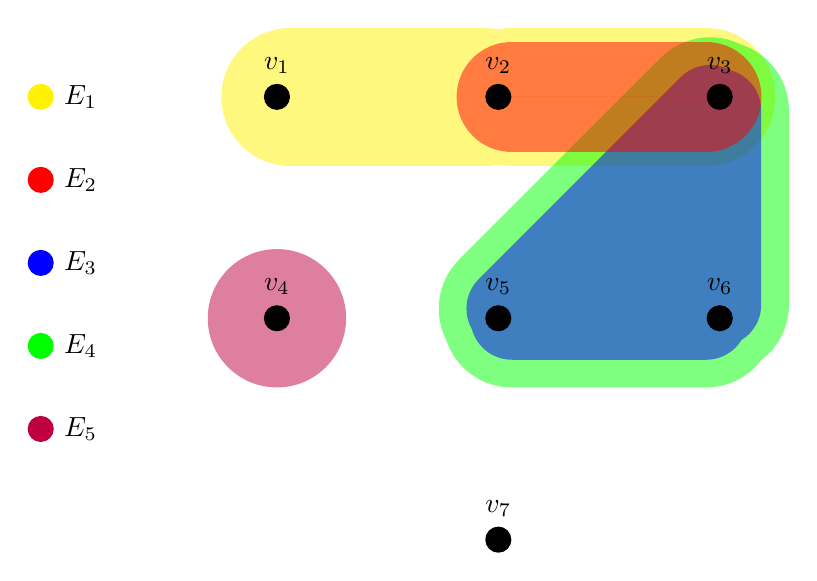
\begin{tikzpicture}
    \tikzstyle{vertex} = [fill,shape=circle,node distance=80pt]
\tikzstyle{edge} = [fill,opacity=.5,fill opacity=.5,line cap=round, line join=round, line width=50pt]
\tikzstyle{edge2} = [fill,opacity=.5,fill opacity=.5,line cap=round, line join=round, line width=30pt]

\tikzstyle{elabel} =  [fill,shape=circle,node distance=30pt]

\pgfdeclarelayer{background}
\pgfsetlayers{background,main}

\node[vertex,label=above:\(v_1\)] (v1) {};
\node[vertex,right of=v1,label=above:\(v_2\)] (v2) {};
\node[vertex,right of=v2,label=above:\(v_3\)] (v3) {};
\node[vertex,below of=v1,label=above:\(v_4\)] (v4) {};
\node[vertex,right of=v4,label=above:\(v_5\)] (v5) {};
\node[vertex,right of=v5,label=above:\(v_6\)] (v6) {};
\node[vertex,below of=v5,label=above:\(v_7\)] (v7) {};

\begin{pgfonlayer}{background}
\draw[edge,color=yellow] (v1) -- (v2) -- (v3);
\begin{scope}[transparency group,opacity=.5]
\draw[edge,opacity=1,color=green] (v3) -- (v5) -- (v6) -- (v3);
\fill[edge,opacity=1,color=green] (v3.center) -- (v5.center) -- (v6.center) -- (v3.center);
\end{scope}

\begin{scope}[transparency group,opacity=.5]
\draw[edge2,opacity=1,color=blue] (v3) -- (v5) -- (v6) -- (v3);
\fill[edge2,opacity=1,color=blue] (v3.center) -- (v5.center) -- (v6.center) -- (v3.center);
\end{scope}
\draw[edge,color=red,line width=40pt] (v2) -- (v3);
\draw[edge,color=purple] (v4) -- (v4);
\end{pgfonlayer}

\node[elabel,color=yellow,label=right:\(E_1\)]  (e1) at (-3,0) {};
\node[elabel,below of=e1,color=red,label=right:\(E_2\)]  (e2) {};
\node[elabel,below of=e2,color=blue,label=right:\(E_3\)]  (e3) {};
\node[elabel,below of=e3,color=green,label=right:\(E_4\)]  (e4) {};
\node[elabel,below of=e4,color=purple,label=right:\(E_5\)]  (e5) {};
\end{tikzpicture}
\end{center}
\end{example}
\begin{definition}
  In a hypergraph $\hgraf=(V,E)$, two vertices $v_i, v_j \in V$ are called 
  \textbf{adjacent} if there is an edge $E_i \in E$ that contains both vertices. 
  Two edges $E_k, E_l$ are called adjacent if their intersection is not empty.
\end{definition}\index{adjacency relation}\index{hypergraph!adjacency relation}

\begin{definition}\index{order}\index{hypergraph!order}
  The \textbf{order of a finite hypergraph $\hgraf$} is the number of vertices of $\hgraf$ 
  and is denoted by $|\hgraf|$.
\end{definition}
We now define the degree of a vertex in a hypergraph. Note that we don't define 
the indegree and outdegree of  a vertex as the hypergraphs we consider are 
undirected.
\begin{definition}\index{degree}\index{hypergraph!degree}
The \textbf{degree of a vertex} $v$ in a hypergraph $\hgraf$ is the number of 
times $v$ is contained in an edge.
\end{definition}

\begin{definition}\index{path}\index{hypergraph!path}\index{length}\index{join}
A \textbf{path} in an hypergraph $\hgraf = (V,E)$ is a sequence $p = (a_0, A_1, a_1, \ldots, A_k, a_k),$ $k \geq 1$ where the
$a_i$'s are pairwise distinct vertices, the $A_i$'s are pairwise distinct
edges and ${a_{i-1}, a_i} \in A_i$ for $1 \leq i \leq k$. The path $p$ is said 
to \textbf{join} $a_0$ and $a_k$. The \textbf{length} of the path is $k$.
\end{definition}

\begin{definition}\index{connected hypergraph}\index{hypergraph!connected hypergraph}
A hypergraph is \textbf{connected} if for each vertex there is a path to any 
other vertex.

\end{definition}
\subsubsection{$k$-hypergraphs}\index{uniform hypergraphs}\index{hypergraph!uniform hypergraphs}
In most applications, the edges of an hypergraph connect a fixed number of 
vertices. 
\begin{definition}\index{$k$-uniform hypergraphs}\index{$k$-graphs}
  An hypergraph is called a \textbf{$k$-uniform hypergraph} for $k \geq 2 \in \N$ if for all $E_i \in E$, 
  the cardinality $|E_i|$ is equal to $k$. The cardinality of multisets is defined in Definition \ref{multiset}.
  The term \textbf{$k$-graph} is often used 
  instead of a $k$-uniform hypergraph. The edges in a $k$-graph are sometimes 
  called $k$-edges.
\end{definition}

Notice that the $2$-hypergraphs are just the undirected graphs we defined in the previous 
section.



\subsubsection{Directed hypergraphs}\index{directed hypergraphs}\index{hypergraph!directed hypergraphs}
An important difference with the previous section is that all hypergraphs we 
have defined are \textbf{undirected}: there is no specific order in which an 
edge connect different vertices. In a graph, directed edges arise naturally as 
some vertex can be the source node and some vertex can be the terminal node, no other nodes
are connected by an edge of a graph. For edges of hypergraphs this concept is not straightforward to generalize: one option is to see 
edges as paths connecting vertices in a specific order,
 another option is to partition the vertices connected by an edge in a set of source 
 nodes and a set of terminal nodes. This last notion is 
studied in \cite{gallo}. We will not discuss this topic in detail, all the 
hypergraphs in this master thesis are undirected.


\subsection{Incidence matrix}\index{incidence matrix}\index{hypergraph!incidence matrix}\index{matrix!incidence matrix}
A hypergraph can be represented as an incidence matrix by numbering the vertices 
and the edges. The resulting incidence matrix will be a boolean matrix with only 
$1$ and $0$ entries. An alternative way to represent a hypergraph is by using
adjacency tensors.

\begin{definition}\label{incidencematrixhypergraph}
  The \textbf{incidence matrix} of a hypergraph $\hgraf = (V, E)$ with vertices
  $v_1, \ldots, v_n \in V$ and edges $e_1, \ldots, e_m \in E$ is a $n\times m$-matrix $A$ 
  where rows represent the vertices and the columns represent the 
  edges, such that:
  
 $$(A)_{ij} = \begin{cases} 1 &\mbox{if } v_i \in e_j   \\ 
0 & \mbox{if } v_i \not\in e_j \end{cases}$$
\end{definition}
\begin{example}
  The corresponding incidence matrix of the hypergraph of Example \ref{vb1hypergraph} 
  is:
  $$\begin{pmatrix}
    1 & 0 & 0 & 0 & 0\\
    1 & 1 & 0 & 0 & 0\\
    1 & 1 & 1 & 1 & 0\\
    0 & 0 & 0 & 0 & 1\\
    0 & 0 & 1 & 1 & 0\\
    0 & 0 & 1 & 1 & 0\\
    0 & 0 & 0 & 0 & 0\\
  \end{pmatrix}.$$
\end{example}







\chapter{Similarity on graphs}

In the previous chapter all the basic terminology and results were introduced.
Now we take an extensive look at the concept of similarity on graphs. Similarity on graphs is a fairly new
concept to compare the nodes of two graphs. The concept arose from the research on algorithms for web searching engines (like \emph{Google}, \emph{Yahoo},\ldots) in the late nineties. 
More specifically, Jon M. Kleinberg 
introduced in his paper `Authoritative Sources in a Hyperlinked Environment' 
\cite{kleinberg} the famous `HITS algorithm' for extracting information from the link structure of websites. The method leads to an iterative algorithm where 
graphs represent the link structure of a collection of websites on a specific topic. Because this paper formed the basis of later research on similarity on graphs, 
the
whole idea and algorithm of Kleinberg is introduced in the first section of this chapter. In 
2004, V.D. Blondel et al. \cite{blondel} generalized the algorithm of 
Kleinberg, introducing the notion of similarity on directed graphs. This similarity is covered in the second section. With this similarity on directed graphs, 
there is a much wider scope of applications than just search algorithms. The method
of Blondel only returns node similarity scores, which are in fact a 
measurement of how similar two nodes of two graphs are to each other, and so in 
the next section, we extend the method of Blondel to both node and edge 
similarity scores. We conclude this chapter with a notion of similarity on 
colored graphs. 

\section{The HITS algorithm of Kleinberg}\index{HITS algorithm}
\subsection{History}
Back in the nineties, internet became more and more popular. The popular search 
engines back then where Altavista and Yahoo, but they weren't as advanced as 
search engines today. The main pitfall of the first search engines was that the search results 
were purely based on the number of occurrences of a word in a webpage. This was 
a pitfall for many reasons. The first reason was the growing popularity of the 
internet: as more and more webpages were put online, simply getting the relevant 
pages to a search query in this text-based manner, was a process that could possibly return millions 
of relevant pages. Also \emph{content similarity}\index{content similarity} was an issue: a website owner 
can easily cheat in a text-based search system by just adding and repeating some 
very popular search words, making his website appear in the results of a large 
number of search queries.
Two possible solutions were simultaneously invented in 1997 and 1998. The first 
one was the
\textit{PageRank}\index{PageRank}\index{Google Pagerank}-system developed by Larry Page and Sergey 
Brin (\cite{page}). The PageRank system led to the foundation of the immensely popular Google 
search engine. Meanwhile, also Jon Kleinberg\index{Kleinberg}\index{Jon Kleinberg} came up with his own solution, the\textit{ HITS algorithm} (hyperlink-induced topic search). At that time,
he was both a professor in the Computer Science Department at the Cornell University and researcher for IBM. The algorithm is 
used inter alia today by the Ask search engine (www.ask.com).
Both these algorithms use the hyperlinks between webpages to rank search 
results. 
Because this master thesis is about similarity and this concept is 
introduced on graphs as a generalization of the HITS algorithm, we don't go into 
further detail about the PageRank algorithm. In the following paragraphs, the 
HITS algorithm is extensively explained.

\subsection{Motivation}\label{motivatiehits}
Kleinberg's work originates in the problems that arise with text-based searching the WWW. Text-based searching just counts all the occurrences of a given search query on webpages and returns a set of webpages ordered by decreasing occurency.
When a user 
supplies a search query, we probably face an \textit{abundance problem}\index{abundance problem} with this method: the number of pages that could reasonably be returned as relevant is
far too large for a human user to digest. To provide effective search results 
under these conditions, we need to filter the `authoritative' ones. We face some complications when we
want to filter the `authoritative' webpages in a text-based system. For example, if we search for `\texttt{job offers in Flanders} 
' the most authoritative page and expected first result in a search engine would be \texttt{www.vdab.be}. 
Unfortunately, the query  `\texttt{job offers}' is used in over a 
million pages on the internet and \texttt{www.vdab.be} is not the one using the 
term most often. Therefore, there is no way to favor \texttt{www.vdab.be} in a 
text-based ranking function. This a recurring phenomenon, e.g., if 
you search for the query `\texttt{computer brands}', there is no reason at all to be sure that the 
website of Apple or Toshiba even contains this search term.

The HITS algorithm solves these difficulties by analyzing the hyperlink 
structure among webpages. The idea is that hyperlinks encode a sort of human 
judgment and that this judgement is crucial to formulate a notion of authority. 
Specifically, when a page $p$ includes a link to page $q$, it means 
that $p$ gives a \textit{conferred authority}\index{conferred authority} on $q$. Again we face difficulties, because this conferred authority doesn't 
hold for every link. Links are created for a wide variety of reasons, for 
example, a large number of links are created for navigation within a website (e.g. ``Return to homepage'') 
and these have of course nothing to do with a notion of authority. 

The HITS method is based on the relationship between the \textit{authorities}\index{authority} for a topic 
and the pages that link to many related authorities, called \emph{hubs}\index{hub}. Page $p$ 
is called an \textit{authority} for the query `\texttt{smartphone brand}' if it 
contains valuable information on the subject. In our example websites of 
smartphone manufacturers such as `\texttt{www.apple.com}', 
`\texttt{www.samsung.com}',... would be good authorities for this search 
query. These are also the results a user would expect from a search engine. 

A hub is a second category of pages needed to find good authorities. Their role 
is to advertise authoritative pages. Hubs contain useful links toward these 
authorities. In our example, consumer websites with reviews on smartphones, 
websites of smartphone shops,\ldots would be good hubs. In fact, hubs point the 
search process in the `right direction'.

To really grasp the idea, we make an analogy with everyday life. If you tell a 
friend that you think of buying a new smartphone, he might tell you his 
experiences with smartphones and he will probably share some opinions he got from other friends. 
He might suggest you some good models and good brands. Now, you are more inclined to 
buy a smartphone that your friend suggested. Well, this idea is used in the 
HITS method: your friend served as a hub, the brands and models he suggested are good 
authorities.

\subsection{Constructing relevant graphs of webpages}
\begin{algorithm}[t!]

\SetAlgoLined
 \KwData{\\$\sigma$: a query string.\\$\mathcal{E}$: a text-based search engine.\\$t$: natural number (usually initiated to $200$)\\
 $d$: natural number (usually initiated to $50$).}
 \KwResult{A page set $S_\sigma$ satisfying all the properties of our wish list.}
\SetKwFunction{creategraph}{create\_graph}
\SetKwProg{myalg}{begin}{}{end}
\myalg{\creategraph{$\sigma$, $\mathcal{E}$, $t$, $d$}}{
 Let $R_\sigma$ denote the top $t$ results of $\mathcal{E}$ on $\sigma$\;
 Set $S_\sigma := R_\sigma$\;
 \For{each page $p \in R_\sigma$}{
 Let $\Gamma^+(p)$ denote the set of all pages $p$ points to\;
 Let $\Gamma^-(p)$ denote the set of all pages pointing to $p$\;
 Add all pages in $\Gamma^+(p)$ to $S_\sigma$\;
 \eIf{$|\Gamma^-(p)| \leq d$}{
 Add all pages in $\Gamma^-(p)$ to $S_\sigma$\;
 }{
 Add an arbitrary set of $d$ pages from $\Gamma^-(p)$ to $S_\sigma$\;
 }
 }
 \KwRet $S_\sigma$\;}{}
 
 \caption{Algorithm to construct $S_\sigma$.}\label{algoritmegraf}
\end{algorithm}
Any collection of hyperlinked pages can be transformed to a directed graph $\graf = (V, 
\to)$: the nodes correspond to the pages, and if there is a link from page $p$ 
to page $q$, there is an arc $p \to q$. Suppose a search query is performed, 
specified by a query $\sigma$. We wish to determine the authoritative 
pages by an analysis of the link structure. But first we have to construct a 
subgraph of the internet on which our algorithm will operate. We want to make the 
computational effort as efficient as possible, so we restrict the subgraph to 
the set $Q_\sigma$ of all pages where the query $\sigma$ occurs. For this, we could use
any already existing text-based search engine.  But, for our algorithm $Q_\sigma$ 
is possibly much too big: it may contain millions of pages making it impossible 
for any computer to preform the algorithm. Moreover it is, as explained in the motivation in \ref{motivatiehits}, possible that $Q_\sigma$ 
does not contain some of the most important authorities because they never use 
the query string $\sigma$ on their website.

Therefore, we wish to transform the set $Q_\sigma$ to a set $S_\sigma$ of pages following 
this `wish list' of properties:
\begin{enumerate}
  \item $S_\sigma$ is relatively small,
  \item $S_\sigma$ is rich in relevant pages,
  \item$S_\sigma$ contains most of the strongest authorities.
\end{enumerate}
By keeping $S_\sigma$ small, the computational cost of preforming 
non-trivial algorithms can be kept under control. By the property of being rich 
in relevant pages, it will be easier to find good authorities. 

To construct $S_\sigma$, we first construct a \emph{root set} $R_\sigma$ with the $t$ highest-ranked pages for $\sigma$ 
using a text-based search engine (they sort results based on the occurence of 
$\sigma$). Typically, $t$ is set about $200$. $R_\sigma$ complies with properties 1 and 2 
of our wish list, but because $R_\sigma \subset Q_\sigma$, it may fail from satisfying 
property 3. Now we use the root set $R_\sigma$ to create the set $S_\sigma$ satisfying our 
complete wish list. When a strong authority is not in $R_\sigma$, it is very 
likely that at least one of the pages in $R_\sigma$ points to this authority. 
Hence, by using the pages in $R_\sigma$, we can expand it to $S_\sigma$ by looking 
at the links that enter and leave $R_\sigma$. We get algorithm \ref{algoritmegraf}.

Thus, we obtain $S_\sigma$ by expanding
$R_\sigma$ to include any page pointed to by a page in $R_\sigma$. We also add $d$ pages that point
to a page in $R_\sigma$. $d$ is usually initiated to 50. The parameter $d$ is 
crucial to stay in accordance with property 1 of our wish list. Indeed, a 
webpage can be pointed to by several thousands and thousands of other webpages, 
and we don't want to include them all if we want to keep $S_\sigma$ relatively 
small. Some experiments in \cite{kleinberg} showed that this algorithm resulted in a $S_\sigma$ 
with a size in the range of 1000 to 5000 web pages. Property 3 of our wish list is usually met 
because a strong authority need only be reference once in the $t$ pages of the 
root set $R_\sigma$ to be added to $S_\sigma$. 

Denote the resulting graph of the page set $S_\sigma$ by $\graf[S_\sigma]$. Note that $\graf[S_\sigma]$ will 
contain 
a lot of links serving only navigational purposes within a website. As mentioned 
before, these links have nothing to do with the notion of authority and they must be 
removed from our final graph if we want a good determination of  the authoritative pages by an analysis of
 the link structure.  A very simple heuristic can be used to derive a subgraph 
 of $\graf[S_\sigma]$ leaving out all the navigational links: we make a 
 distinction between \emph{transverse} links and \emph{intrinsic} links. 
 Transverse links are links between different domain names (e.g. a link between \texttt{www.vub.ac.be} and
 \texttt{www.ua.ac.be}) and intrinsic links are links between the same domain 
 name (e.g. a link between \texttt{www.vub.ac.be} and
 \texttt{dwis.vub.ac.be}). Intrinsic links exist to allow navigation within a 
 website and they tell us very little about the authority of the pages they 
 point to. Therefore, we delete all intrinsic links from  $\graf[S_\sigma]$, 
 keeping only the arcs corresponding to transverse links.
 
Our graph still contains some meaningless links in the context of page 
 authority. Suppose a large number of pages from the same domain name have a transverse link to 
 the same page $p$. Most of the time, this means a form of advertisement (by example `Website created by\ldots.' at the bottom of each page). It is useful 
 to only allow $m$ pages ($m$ is usually initiated to 6) from the same domain name to have a transverse link to the same page. 
 If $m$ is exceeded, all the transverse links must be deleted from the graph. Note, 
 however, that not all links to advertisements will be erased because on most 
 web pages, advertisements change on every page which avoids the exceeding of $m$.
 
 Applying the two described heuristics above on $\graf[S_\sigma]$, we get a new 
 graph $\graf'_\sigma$ which is exactly what we need to preform our link analysis.
 
 \subsection{Hubs and Authorities}\index{hub} \index{authority}
 A very simple approach would now be to order the pages in $\graf'_\sigma$ by 
 their indegree. Although this approach can sometimes return good search results, this
 heuristic is often too simple because $S_\sigma$ will probably contain some 
 web pages with a lot of incoming links without being very relevant to the search query $\sigma$ (e.g. advertisements).   
 With these incoming links, those web pages are ranked high in the final search 
 result, which we want to avoid.

 Do we have to return to a text-based approach to avoid irrelevant web pages 
 being on top of the search results? No, the link structure of $\graf'_\sigma$ 
 can tell us a lot more than it may seem at first glance.  Authoritative pages 
 relevant to query $\sigma$ should indeed have a large in-degree, but there should also be a considerable overlap in the sets 
 of pages that point to authoritative pages. This set of pages that point to 
 authoritative pages are called \textit{hubs}. Hubs have links to several 
 authoritative pages and they sort of ``concentrate'' all the authorities on 
 query $\sigma$. Figure \ref{hubauth} shows what this means conceptually.
 \begin{figure}[h!]
  \centering
  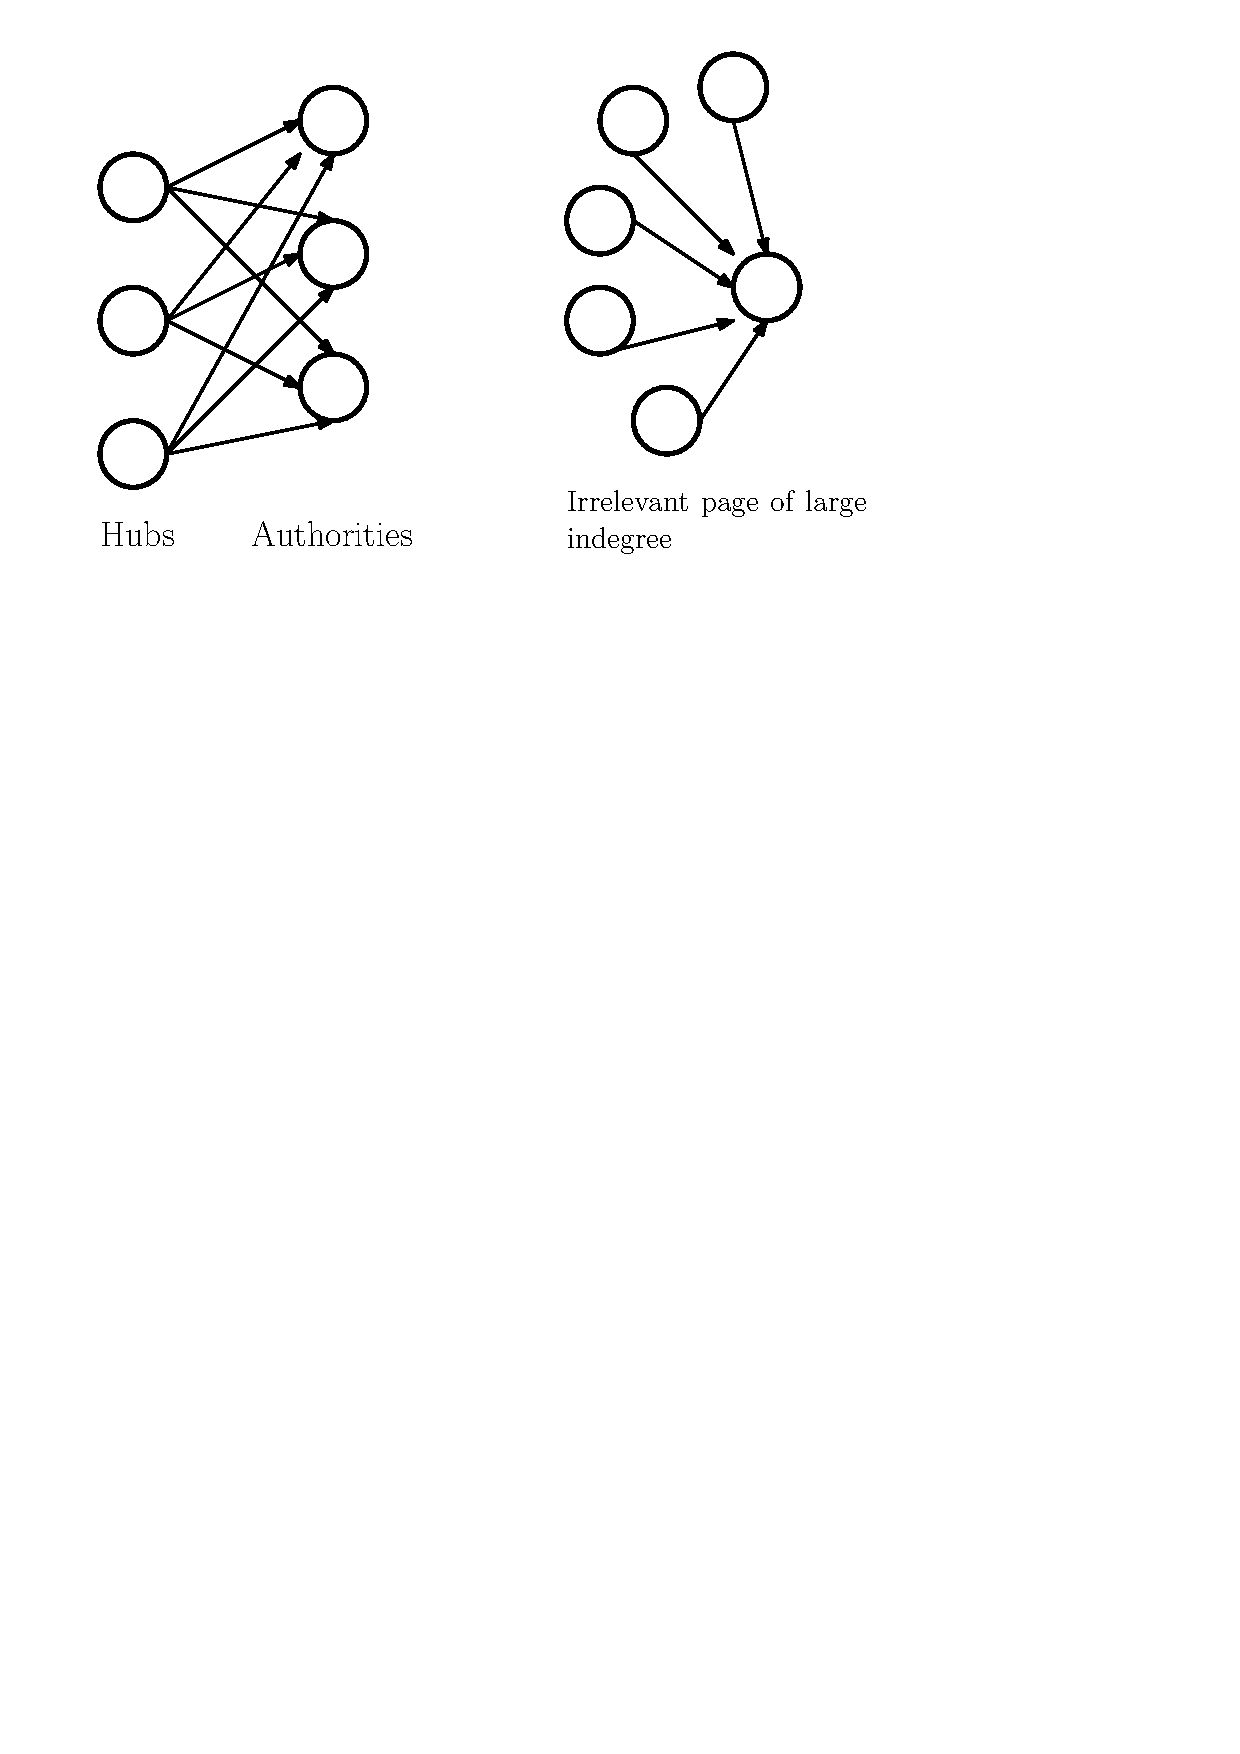
\includegraphics[scale=1]{fig1hits.pdf}\caption{The concept of hubs and authorities}\label{hubauth}
\end{figure}
 
 So, for each page $j$ we assign two scores, an \textit{authority score} 
 which estimates the value of the content of the page and a \textit{hub 
 score} which estimates the value of the outgoing links to other pages. We now get a dichotomy: a good hub is a page pointing to many good authorities, a good 
 authority is a page that is pointed to by many good hubs. This leads us to a 
 \textit{mutually reinforcing relation} \index{mutually reinforcing relation} resulting in an iterative method to 
 break this circularity.
 
So let $\graf'_\sigma = (V,\to)$ and let $h_j$ and $a_j$ be the hub and authority 
scores of vertex $v_j$ (corresponding with page $j$). These scores must be initialized by some positive start values 
and then updated simultaneously for all vertices. This leads to a \emph{mutually reinforcing relation} 
in which the hub score of $v_j$ is set equal to the sum of the authority scores of all 
vertices pointed to by $v_j$ and in an equal manner the authority score of $v_j$ 
is set equal to the sum of the hub scores of all vertices pointing to $v_j$.

$$\begin{cases} h_j := \sum_{i:(v_j,v_i)\in \to} a_i,\\ 
a_j := \sum_{i:(v_i,v_j)\in \to} h_i.
\end{cases}$$ 

The basic operations in which hubs and authorities reinforce one another are 
depicted in Figure \ref{reinforcing}.

\begin{figure}[h!]
  \centering
  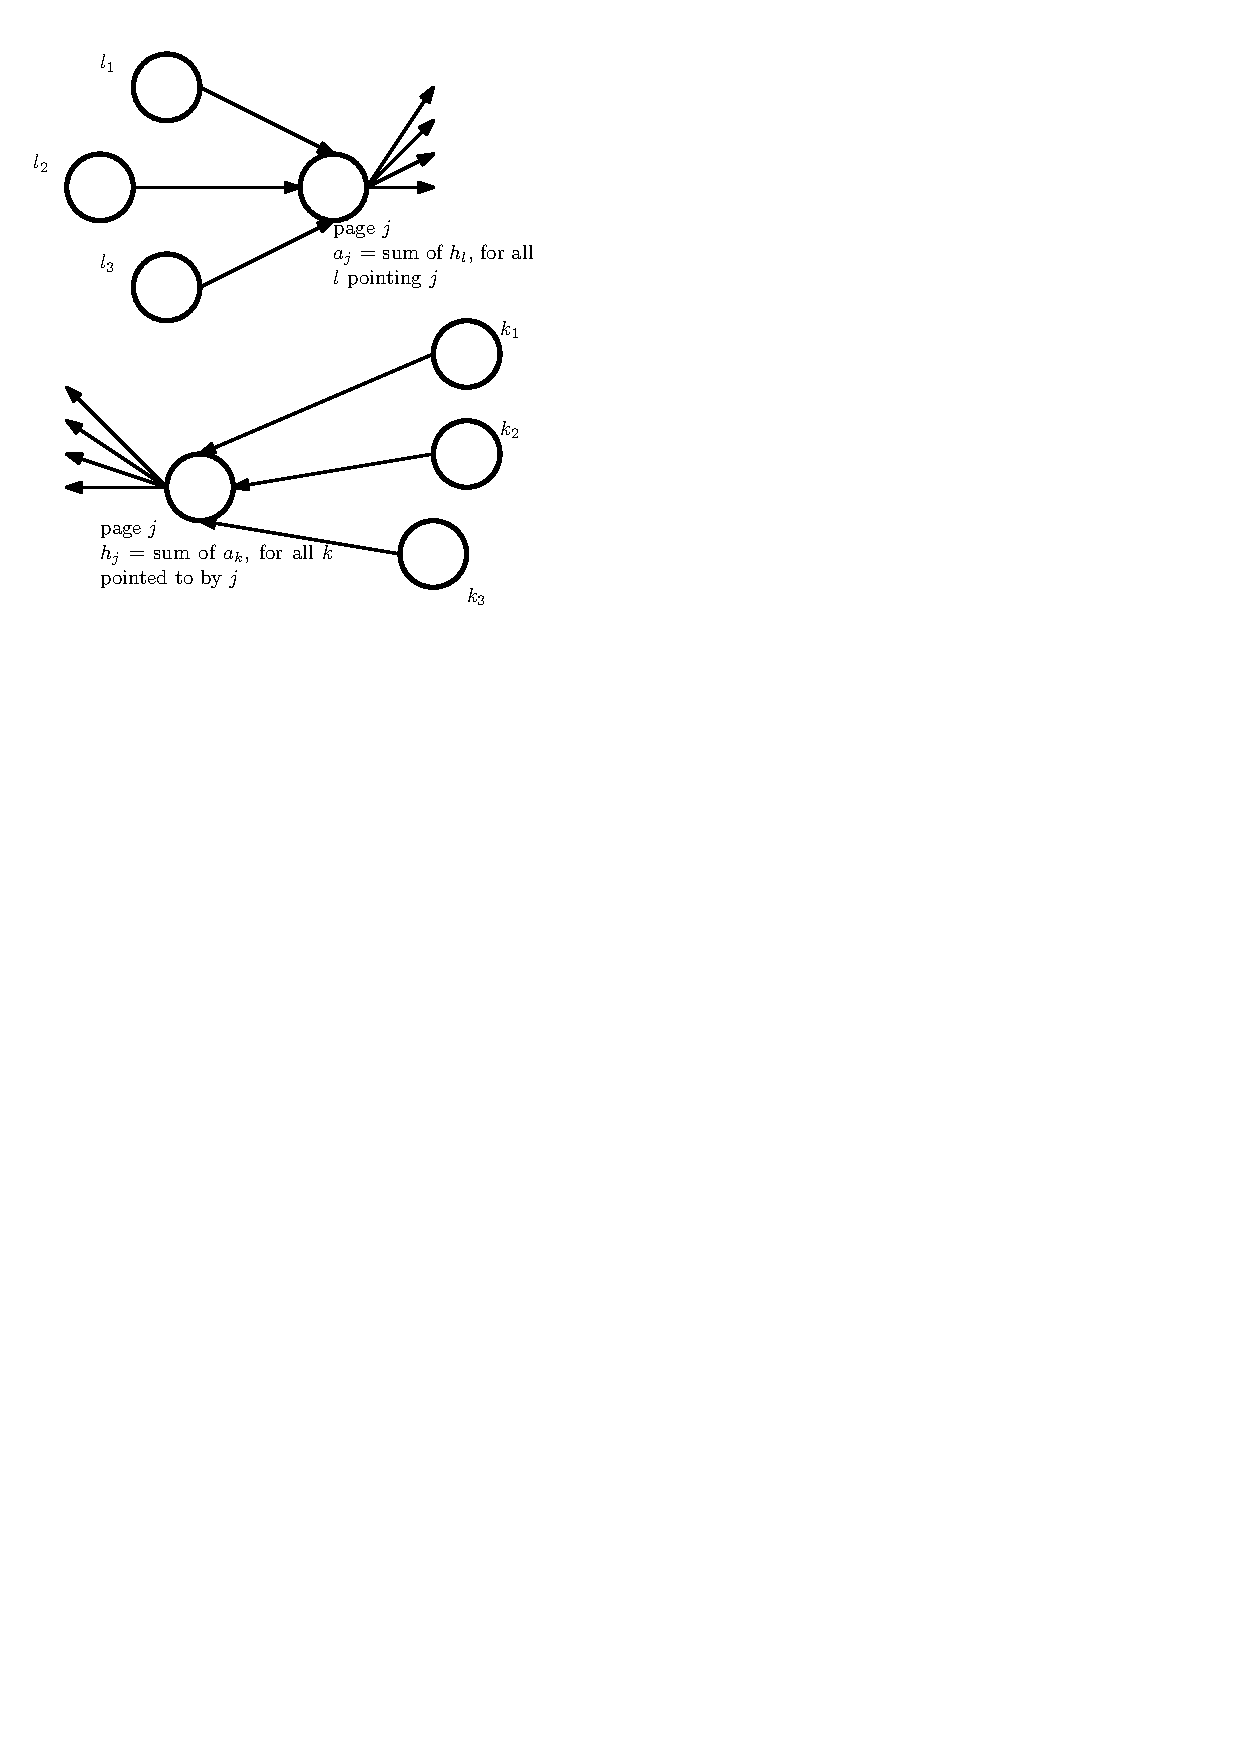
\includegraphics[scale=1]{fig2hits.pdf}\caption{The basic operations in the reinforcing relation between hubs and authorities}\label{reinforcing}
\end{figure}

Let $B$ be the adjacency matrix of $\graf'_\sigma$ and denote $\mathbf{a}$ as the authority vector with coordinates $(a_1,a_2,\ldots,a_n)$ (with $n = 
 |\graf'_\sigma|$, the number of pages) and $\mathbf{h}$ as the hub vector. The mutually reinforcing relation can now be rewritten 
as:

$$\begin{pmatrix} 
\textbf{h}\\
\textbf{a}
\end{pmatrix}^{(k+1)} = \begin{pmatrix} 
0 & B\\
B^T & 0
\end{pmatrix} \begin{pmatrix} 
\textbf{h}\\
\textbf{a}
\end{pmatrix}^{(k)},\quad k = 0, 1,\ldots,$$
In compact form, we denote
\begin{eqnarray}\label{compactform}
  \mathbf{x}^{(k+1)} = M\mathbf{x}^{(k)},\quad k = 0, 1,\ldots,
\end{eqnarray}

where 
$$\mathbf{x}^{(k)} = \begin{pmatrix} 
\mathbf{h}\\
\mathbf{a}
\end{pmatrix}^{(k)}, M =  \begin{pmatrix} 
0 & B\\
B^T & 0
\end{pmatrix}$$

After each iteration, we have to normalize $h_j$ and $a_j$. Indeed, we want to get the authority and hub weights for each page
and in order to compare these after each iteration step, they must be normalized because only the relative differences do matter, otherwise the whole procedure would be 
meaningless. Pages with larger $a_j$-scores are viewed as being better authorities, pages with larger $h_j$-scores are better hubs. 

We get the following sequence (with $z^{(0)}$ some positive start value) of normalized vectors: 
\begin{eqnarray}\label{sequencezk}
  \mathbf{z}^{(0)} = \mathbf{x}^{(0)} > 0, \mathbf{z}^{(k+1)} = \frac{M\mathbf{z}^{(k)}}{||M\mathbf{z}^{(k)}||_2}, \quad k = 
  0,1,\ldots,
\end{eqnarray}

How do we decide on $\mathbf{x}^{(0)}$? We will see that any positive vector in $\R^{2n}$ is a good choice, but for the sake of simplicity, we make the natural choice\footnote{$\mathbf{1}$ is a matrix, or vector, whose entries are all equal to 
$1$.} $\mathbf{1} \in \R^{2n}$ . The limit to which the sequence converges 
results in `definitive' hub and authority scores for each page in the graph $\graf'_\sigma$. 

To compute the iterative algorithm, we update the hub and authority scores in an alternating form (by each step we have to normalize the scores). 
Because we will prove that the sequence converges, theoretically we can keep on iterating until a fixed point is approximated. But in most practical settings, 
we choose a fixed number of steps $k$ to reduce the computational cost because we cannot know beforehand how
large $k$ has to be to reach the limit. But of course, it is extremely important to know that method converges anyway. Let $\mathbf{x}^{(i)}$ denote vector $\mathbf{x}$ at iteration step $i$ as in Notation \ref{numeriekenotatie}, and we get Algorithm 
\ref{hitsalgorithm}.


\begin{algorithm}[t!]
 \KwData{\\$\graf$: a graph of $n$ linked pages.\\$k$: natural number.}
 \KwResult{A vector $(\mathbf{h}, \mathbf{a})$ containing the hub and authority scores after $k$ steps.}
\SetKwFunction{hits}{hits}
\SetKwProg{myalg}{begin}{}{end}
\myalg{\hits{$\graf$, $k$}}{
 Set $\mathbf{a}^{(0)} = (1,1,\ldots,1) \in \R^n$\;
 Set $\mathbf{h}^{(0)} = (1,1,\ldots,1) \in \R^n$\;
 \For{$i = 1, 2,\ldots,k$}{
 Calculate  $\mathbf{h'}^{(i)} = \left(\sum_{m:(v_1,v_m)\in \to} \mathbf{a}^{(i-1)}_{m}, \sum_{m:(v_2,v_m)\in \to}  \mathbf{a}^{(i-1)}_{m},\ldots, \sum_{m:(v_n,v_m)\in \to}  
 \mathbf{a}^{(i-1)}_{m}\right)$\;
 Normalize  $\mathbf{h'}^{(i)}$ obtaining $\mathbf{h}^{(i)}$\;
 Calculate $\mathbf{a'}^{(i)}=\left(\sum_{m:(v_m,v_1)\in \to} \mathbf{h}^{(i)}_m, \sum_{m:(v_m,v_2)\in \to} \mathbf{h}^{(i)}_m, \ldots, \sum_{m:(v_m,v_n)\in \to} 
 \mathbf{h}^{(i)}_m\right)$\;
 Normalize  $\mathbf{a'}^{(i)}$ obtaining $\mathbf{a}^{(i)}$\;
}

 \KwRet $(\mathbf{h}^{(k)},\mathbf{a}^{(k)} )$\;}{}
 
 \caption{The iterative HITS algorithm.}\label{hitsalgorithm}
\end{algorithm}

To filter the top $c$ hubs and the top $c$ authorities, you can use the trivial 
Algorithm \ref{filter}. \begin{algorithm}[t!]
 \KwData{\\$\graf$: a graph of $n$ linked pages.\\$k$: natural number.\\$c$: natural number.}
 \KwResult{A vector $((\mathcal{H}_1,\mathcal{H}_2,\ldots, \mathcal{H}_c), (\mathcal{A}_1,\mathcal{A}_2,\ldots, \mathcal{A}_c))$ containing exactly the nodes of the $c$ top hubs and $c$ top authorities.}

\SetKwFunction{filter}{filter}
\SetKwFunction{hits}{hits}

\SetKwProg{myalg}{begin}{}{end}
\myalg{\filter{$\graf$, $k$, $c$}}{
$(\mathbf{h},\mathbf{a}) =$ \hits{$\graf$, $k$}\;
Sort the pages with the $c$ largest values in $\mathbf{h}$, resulting in 
a vector of nodes $(\mathcal{H}_1,\mathcal{H}_2,\ldots, \mathcal{H}_c)$\;
Sort the pages with the $c$ largest values in $\mathbf{a}$, resulting in 
a vector of nodes $(\mathcal{A}_1,\mathcal{A}_2,\ldots, \mathcal{A}_c)$\;

 \KwRet $((\mathcal{H}_1,\mathcal{H}_2,\ldots, \mathcal{H}_c), (\mathcal{A}_1,\mathcal{A}_2,\ldots, \mathcal{A}_c))$\;}{}
 
 \caption{Returning the top $c$ hubs and authorities}\label{filter}
\end{algorithm}

How do we decide on the values of $k$ and $c$? It is immediately clear that $c$ and $k$ must
be proportional: for low $c$ values, a lower 
value for the number of iteration steps $k$ is appropriate and vice versa. 
Experiments in \cite{kleinberg} showed that $k$ set to $20$ is sufficient to 
become stable for finding the $5$ best hubs and authorities, thus for $c = 5$. 

\subsection{Convergence of the algorithm}\index{convergence}
We now want to prove that for arbitrarily large values of $k$, the
sequence $Z^{(k)}$ converges to a limit $(\mathbf{h'}, \mathbf{a'})$. Before 
  proving the convergence, note that  adjacency matrices are nonnegative by definition, and thus the matrix $M$ is 
nonnegative too. $M$ is also clearly a symmetric $n' \times n'$-matrix with nonnegative, real entries. We prove that such matrices
have  $n'$ (not necessarily different) real eigenvalues and that we can diagonalize $M$.   This is the first condition of the  
power method we introduced in section \ref{powersection}.
If we can also prove the second condition (having a unique dominant eigenvalue), 
convergence is immediately shown by the power method.

However, there is a problem here: we cannot prove that nonnegative symmetric matrices have a unique dominant 
eigenvalue (a unique dominant eigenvalue means the largest eigenvalue with multiplicity 1), simply because this is not true in general.\footnote{The matrix $\begin{pmatrix} 
1 & 0\\
0 & 1
\end{pmatrix}$ is a simple counterexample of a symmetric, nonnegative, real matrix that has no unique dominant eigenvalue.} 
In the original paper of Kleinberg \cite{kleinberg} he solves this issue by 
simply imposing that the matrix $M$ has a unique dominant eigenvalue and he doesn't pay any further attention to this problem.  
He presents it as `a small, technical assumption for the sake of simplicity'.

Is this justified in practice? Actually it is, because you can prove with probability theory that a random 
matrix $C_n$,  with a probability tending to 1, has no repeated eigenvalues as the size of the matrix goes to infinity (See for example Thereom 2.2.3 in \cite{random}).  You can also defend this differently: the only reason why we can't use the 
Perron-Frobenius theorem (see \ref{frobtheorem}) here, is because $M$ will have 
zero entries (not all pages in $S_\sigma$ will be linked to each other, the graph $\graf'_\sigma$ is not strongly connected in general). But,
it is intuitively clear that by adding 1 to each entry of $M$, the final results 
of the algorithm (a sorted vector with the best hubs and authorities) will not 
be changed at all, because pages with larger indegrees and outdegrees will continue to get better hub and authority scores (note, however, that the relative hub and authority scores can fluctuate a bit and the algorithm will converge slower because of the lack of zero 
entries). So, by adding 1 to each entry of $M$, the matrix becomes a positive, real matrix 
and we know from the Perron-Frobenius that these matrices have a unique dominant 
eigenvalue. So yes, the `small, technical assumption' in the paper of Kleinberg 
is justified.

Now that this problem is solved, we present the relevant theorems below. We also 
impose on the matrix $M$ that it has a unique dominant eigenvalue with the preceding explanations in mind. 
Remember that we will generalize the idea of the HITS algorithm to introduce 
similarity on graphs. Therefore, we will reconsider the 
convergence of the generalized algorithm in the following section. We will prove that there also exists a limit even when the matrix $M$ has no unique 
dominant eigenvalue. We don't present this result immediately,  
because we want to present the results as authentic as possible and we want to show 
the evolution of the ideas in the successive papers.

\begin{theorem}
  If $A$ is a symmetric, real $n\times n$-matrix, then it has $n$ (not necessarily different) real eigenvalues corresponding
  to real eigenvectors.
  \end{theorem}
  \begin{proof}
    First, threat $A$ as complex matrix.
    The characteristic polynomial $\det(A-\lambda I)$ has $n$ roots in $\C$ and 
    each root is an eigenvalue for $A$. Let $\lambda \in \C$ be any eigenvalue 
    and $\mathbf{v} \in \C^n$ be a corresponding eigenvector for $A$. We have:
    $$A\mathbf{v} = \lambda\mathbf{v}.$$ As $A = A^t$, we also get:
    $$\mathbf{v}^tA = \lambda \mathbf{v}^t.$$
    Taking the complex conjugate of both sides we get ($A$ is a real matrix):
    $$\bar{\mathbf{v}}^tA = \bar{\lambda}\bar{\mathbf{v}}^t$$
    We get:
    $$\bar{\mathbf{v}}^tA\mathbf{v} = (\bar{\mathbf{v}}^tA)\mathbf{v} = (\bar{\lambda}\bar{\mathbf{v}}^t)\mathbf{v} 
    = \bar{\lambda}\bar{\mathbf{v}}^t\mathbf{v}.$$
    We also have:
    $$\bar{\mathbf{v}}^tA\mathbf{v} = \bar{\mathbf{v}}^t(A\mathbf{v}) = 
    \lambda\bar{\mathbf{v}}^t\mathbf{v}.$$
    Hence:
    $$\bar{\lambda}\bar{\mathbf{v}}^t\mathbf{v} = \lambda\bar{\mathbf{v}}^t\mathbf{v}.$$
    We conclude that $\lambda = \bar{\lambda}$ for $\mathbf{v} \not = 0$. 
    We proved that every eigenvalue of $A$ is real. If $\lambda$ is an 
    eigenvalue of $A$, then the matrix $(A - \lambda I)$ is not invertible so a 
    vector $\mathbf{s} \in \R^n$ exists with $$(A - \lambda I)\mathbf{s} = 0,$$ 
    proving that also the corresponding eigenvector is real.
    
  \end{proof}
\begin{theorem}\label{diagonaal}\index{Schur decomposition}\textbf{(Symmetric Schur Decomposition)}
  Let $A$ be a real symmetric matrix, then there exist an orthogonal 
  matrix $P$ such that:
  \begin{enumerate}
    \item[(i)] $P^{-1}AP = D$, a diagonal matrix,
    \item[(ii)] The diagonal entries of $D$ are the eigenvalues of $A$,
    \item[(iii)] The column vectors of $P$ are the eigenvectors of the 
    eigenvalues of $A$.
  \end{enumerate}
\end{theorem}
 \begin{proof}
By induction on the order of the matrix. For $n=1$ the theorem is trivial. Let $A$ 
be a symmetric $n\times n$-matrix. $A$ has at least one eigenvalue $\lambda_1$ by the 
previous theorem. Let $\mathbf{x_1}$ be a corresponding eigenvalue with $\|\mathbf{x}_1\|=1$ 
and $A\mathbf{x}_1=\lambda_1\mathbf{x}_1$. By the Gram-Schmidt procedure, we construct an 
orthonormal basis $V_1 = \{\mathbf{x}_1, \mathbf{v}_2,\ldots,\mathbf{v}_n\}$ of 
$\R^n$.
Let:
$$S_1= [\mathbf{x}_1,\mathbf{v}_2,\ldots,\mathbf{v}_n],$$
since $S_1$ is orthonormal, we get $S^t_1 = S^{-1}$. Consider the matrix:
$S_1^{-1}AS_1$. We have:
$$(S_1^{-1}AS_1)^t = (S_1^{t}AS_1)^t = S_1^t A^t S_1 = S^{-1}_1AS_1$$
Thus $S_1^{-1}AS_1$ is a symmetric matrix. Since $S_1\mathbf{e}_1 = \mathbf{x}_1$, we get:
\begin{eqnarray*}
 S_1^{-1}AS_1\mathbf{e}_1 &=& (S_1^{-1} A)(\mathbf{x}_1)\\
 &=& S_1^{-1}(\lambda_1\mathbf{x}_1)\\
 &=& \lambda_1(S_1^{-1}\mathbf{x}_1)\\
 &=& \lambda_1 \mathbf{e}_1
\end{eqnarray*}
So we get:
$$S_1^{-1}AS_1=\left(
\begin{array}{c|c}
\lambda_1 & \mathbf{0} \\ \hline
\mathbf{0}^t & A_1
\end{array}\right),$$
with $\mathbf{0}$ a vector of zero entries of size $n-1$ and $A_1$ an $(n-1)\times(n-1)$ symmetric matrix. 
We know by induction that there exist a $(n-1)\times(n-1)$ orthogonal matrix $S_2$ such that 
$S_2^{-1}A_1S_2 = D'$ with $D'$ an  $(n-1)\times(n-1)$ diagonal matrix. Let:
$$S'_2=\left(
\begin{array}{c|c}
1 & \mathbf{0} \\ \hline
\mathbf{0}^t & S_2
\end{array}\right),$$
and also $S'_2$ is an orthogonal matrix, we get:
\begin{eqnarray*}
 \left(S'_2\right)^{-1}S_1^{-1}A S_1 S'_2 &=& \left(
\begin{array}{c|c}
1 & \mathbf{0} \\ \hline
\mathbf{0}^t & S^t_2
\end{array}\right) \left(S_1^{-1}A S_1\right) \left(
\begin{array}{c|c}
1 & \mathbf{0} \\ \hline
\mathbf{0}^t & S_2
\end{array}\right) \\
&=& \left(
\begin{array}{c|c}
1 & \mathbf{0} \\ \hline
\mathbf{0}^t & S^t_2
\end{array}\right) 
\left(
\begin{array}{c|c}
\lambda_1 & \mathbf{0} \\ \hline
\mathbf{0}^t & A_1
\end{array}\right) 
 \left(
\begin{array}{c|c}
1 & \mathbf{0} \\ \hline
\mathbf{0}^t & S_2
\end{array}\right) \\
&=& 
 \left(
\begin{array}{c|c}
\lambda_1 & \mathbf{0} \\ \hline
\mathbf{0}^t & S^t_2A_1S_2
\end{array}\right) \\
&=&
 \left(
\begin{array}{c|c}
\lambda_1 & \mathbf{0} \\ \hline
\mathbf{0}^t & D'\end{array}\right) 
\end{eqnarray*}
Thus, if we put
\begin{eqnarray*}
P &=& S_1S'_2\\
D &=& \left(
\begin{array}{c|c}
\lambda_1 & \mathbf{0} \\ \hline
\mathbf{0}^t & D'\end{array}\right),
\end{eqnarray*}
we have proved (1). From the definition of diagonalizable matrices and the fact 
that a square matrix is diagonalizable if and only if it has an eigenbasis (a basis containing only lineair independent 
eigenvectors),
(ii) and (iii) immediately follow.
\end{proof}
 \begin{theorem}
   Giving a graph $\graf$ with $n$ linked pages, the sequence as defined in the previous paragraph: 
   $$\mathbf{z}^{(0)} = \mathbf{1} \in \R^{n}, \mathbf{z}^{(k+1)} = \frac{M\mathbf{z}^{(k)}}{||M\mathbf{z}^{(k)}||_2}, \quad k = 
  0,1,\ldots,$$
  converges when $M$ has a unique dominant eigenvalue.
 \end{theorem}
\begin{proof}
  Since 1) $M$ is diagonalizable as symmetric matrix by Theorem \ref{diagonaal}  
  and 2) $M$ has a unique dominant eigenvalue, it follows from the power method that
  the sequence will converge to a corresponding dominating eigenvector $(\mathbf{h'}, \mathbf{a'})$. This eigenvector contains the hub and authority scores.
  \end{proof}


We conclude with a nice corollary.

\begin{corollary}
The second power of the matrix $M$ has the form:
$$M^2 = \begin{pmatrix} 
BB^T & 0\\
0 & B^TB
\end{pmatrix},$$
and the normalized hub and authority scores are given by the 
dominant eigenvectors of $BB^T$ and $B^TB$.\end{corollary}
 
 \begin{proof}
     By the compact form given in equation \ref{compactform}, we see that $\mathbf{h_k} \leftarrow (BB^T)^{k-1}B\mathbf{a_0}$ 
     and $\mathbf{a_k} \leftarrow (B^TB)^{k}\mathbf{a_0}$. Let $\mathbf{a_0}$ be $\mathbf{1} \in \R^n$. From the previous theorem we 
     also know that:
     $$\lim_{k\to\infty}\mathbf{h_k} = \mathbf{h} \quad \text{and} \quad \lim_{k\to\infty}\mathbf{a_k} = \mathbf{a},$$
     and also from the previous proof we know that $(\mathbf{h}, \mathbf{a})$ is 
     the dominant eigenvector of $M$. It follows immediately that
     $\mathbf{h}$ is also the dominant eigenvector of $BB^T$ and $\mathbf{a}$ is the dominant eigenvector of 
     $B^TB$.
 \end{proof}
 \subsection{Examples}
 \subsubsection{Searching for math professors at the VUB}
\begin{example}
  We conclude this section with a fictitious example of the HITS algorithm. Suppose you 
  are looking for \texttt{math professors vub} with a text-based search engine 
  and you get the following results:
  \begin{itemize}
    \item The website of the mathematics department of the VUB,
       \item The website of the faculty of science of the VUB,
    \item The websites of 4 math professors,
    \item The website of 10 PhD students at the the mathematics department of the VUB.
  \end{itemize}
Lets take a look at the link structure of these web pages (remember that it is a fictitious example):
  \begin{itemize}
    \item The website of the mathematics department at the VUB links to the websites of all the 4 professors, 
    the 10 PhD students and the faculty of science,
   
      \item The website of the faculty of science of the VUB links to the websites 
    of all the 4 math professors and the mathematics department,
    
 \item The websites of the 4 math professors link to the website of the 
    Mathematics department and the faculty of science,

    \item The websites of the 10 PhD students at the the VUB link to the the 
    website of their promotor. 1 professor has 4 PhD students, the other 3 professors 
    have 2 PhD students.
      \end{itemize}
We can now construct the graph $\graf_\sigma$ (of course this graph is not completely made according to Algorithm \ref{algoritmegraf}) and we have the following adjacency matrix of 
$\graf_\sigma$:
\setcounter{MaxMatrixCols}{20}
\begin{itemize}
  \item \textbf{Row 1}: website of the mathematics department,
    \item \textbf{Row 2}: website of the faculty of science,
    \item  \textbf{Row 3}: website of the professor with the 4 PhD students,
    \item  \textbf{Row 4, 5, 6}: websites of the professors with the 2 PhD students,
    \item  \textbf{Row 7, 8, 9, 10}: websites of the 4 PhD students of the professor on row 3,
    \item  \textbf{Row 11, 12}: websites of the 2 PhD students of the professor on row 4,
    \item  \textbf{Row 13, 14}: websites of the 2 PhD students of the professor on row 5,
    \item  \textbf{Row 15, 16}: websites of the 2 PhD students of the professor on row 6,


\end{itemize}
Leads to:
$$
 B= \begin{pmatrix} 
0 & 1 & 1 & 1 & 1 & 1 & 1 & 1 & 1 & 1 & 1  & 1 & 1 & 1 & 1 & 1\\
1 & 0 & 1 & 1 & 1 & 1 & 0 & 0 & 0 & 0 & 0 & 0 & 0 & 0 & 0 & 0 \\
1 & 1 & 0 & 0 & 0 & 0 & 0 & 0 & 0 & 0 & 0 & 0 & 0 & 0 & 0 & 0 \\
1 & 1 & 0 & 0 & 0 & 0 & 0 & 0 & 0 & 0 & 0 & 0 & 0 & 0 & 0 & 0 \\
1 & 1 & 0 & 0 & 0 & 0 & 0 & 0 & 0 & 0 & 0 & 0 & 0 & 0 & 0 & 0 \\
1 & 1 & 0 & 0 & 0 & 0 & 0 & 0 & 0 & 0 & 0 & 0 & 0 & 0 & 0 & 0 \\
0 & 0 & 1 & 0 & 0 & 0 & 0 & 0 & 0 & 0 & 0 & 0 & 0 & 0 & 0 & 0 \\
0 & 0 & 1 & 0 & 0 & 0 & 0 & 0 & 0 & 0 & 0 & 0 & 0 & 0 & 0 & 0 \\
0 & 0 & 1 & 0 & 0 & 0 & 0 & 0 & 0 & 0 & 0 & 0 & 0 & 0 & 0 & 0 \\
0 & 0 & 1 & 0 & 0 & 0 & 0 & 0 & 0 & 0 & 0 & 0 & 0 & 0 & 0 & 0 \\
0 & 0 & 0 & 1 & 0 & 0 & 0 & 0 & 0 & 0 & 0 & 0 & 0 & 0 & 0 & 0 \\
0 & 0 & 0 & 1 & 0 & 0 & 0 & 0 & 0 & 0 & 0 & 0 & 0 & 0 & 0 & 0 \\
0 & 0 & 0 & 0 & 1 & 0 & 0 & 0 & 0 & 0 & 0 & 0 & 0 & 0 & 0 & 0 \\
0 & 0 & 0 & 0 & 1 & 0 & 0 & 0 & 0 & 0 & 0 & 0 & 0 & 0 & 0 & 0 \\
0 & 0 & 0 & 0 & 0 & 1 & 0 & 0 & 0 & 0 & 0 & 0 & 0 & 0 & 0 & 0 \\
0 & 0 & 0 & 0 & 0 & 1 & 0 & 0 & 0 & 0 & 0 & 0 & 0 & 0 & 0 & 0 \\
\end{pmatrix},$$

Intuitively, we expect that the professor with his 4 PhD 
student will have the largest authority score, immediately followed by the other 3 professors.
The website of the mathematics department is clearly the best hub in this example and should get the largest hub score.
Also the website of the faculty of science should get a high hub score.

We now apply the HITS method by
calculating the dominant eigenvector of $BB^T$ (this returns the hub scores) 
and the dominant eigenvector of $B^TB$ (this returns the authority scores) with 
the power method (see \ref{powersection}). We get:


$$ \mathbf{a} = \begin{pmatrix}
0.1979\\
0.3162\\
\mathbf{0.3688}\\
0.3231\\
0.3231\\
0.3231\\
0.2029\\
0.2029\\
0.2029\\
0.2029\\
0.2029\\
0.2029\\
0.2029\\
0.2029\\
0.2029\\
0.2029\\
\end{pmatrix} \quad \text{and} \quad
\mathbf{h} = \begin{pmatrix}
\mathbf{0.8645}\\
0.3605\\
0.1207\\
0.1207\\
0.1207\\
0.1207\\
0.0866\\
0.0866\\
0.0866\\
0.0866\\
0.0758\\
0.0758\\
0.0758\\
0.0758\\
0.0758\\
0.0758\\
\end{pmatrix}
$$

We see that the websites of the 4 math professors are indeed the best authorities for the search 
query \texttt{math professors vub} and that the website of the mathematics department is an 
extremely good hub (this is very logic because it links to all the other relevant 
websites). The professor with his 4 PhD students would be ranked first in the 
search results (he has the highest authority score), the other professors would 
appear just underneath him. Obviously, a hub score of 0.8645 is so high that it would be quite exceptional in 
a graph containing a lot more websites (it is very unlikely that you find a website containing links to all the other pages/nodes in the graph). Nevertheless, we conclude that the HITS algorithm returns the 
results we wanted intuitively.

\end{example}
 \subsubsection{Predictors in the Eurovision Song Contest 
 2009-2015}\index{predictor}\index{Eurovision}
 The Eurovision Song Contest is an annual competition between countries whose 
 public broadcaster is part of the EBU-network. The contest is the biggest music 
 competition in the world, reaching about 200 million annually.
  
 The contest consists of three shows: 2 semi-finals and 1 grand final. From each 
 semi-final, 10 countries proceed the the grand final. Italy, Germany, Spain, United Kingdom and France are 
 always qualified for the grand final because they are the main funders of the event. 
 Also the winner of last year participates automatically in the final. Each country, also those 
 who dropped out during the semi-finals, gives points during the voting of the grand final. 
The voting during the grand final takes place after all the countries have performed their song. 
Each country is called and awards 12 points to their 
favorite song, 10 points to their second favorite, and then points from 8 down 
to 1 to eight other songs. Countries cannot vote for themselves. 

The voting 
system is in fact a positional voting system that is very similar to the Borda count 
method (see \cite{saari} for a scientific explanation of Borda count): the list 
of points of a country represents the ranking of the 10 best countries in the voting of that country. 
So the points are values on an ordinal scale.

The complete voting procedure during the Eurovision Song Contest can be seen as 
a directed graph: all the participating countries are the nodes and the edges 
represent the points between the countries (when country $a$ assigns 3 points to country $b$, then there are 3 edges from $a$ to 
$b$).

Let $A$ be the adjacency matrix of the voting during a song contest ($A$ will in fact be just a points table). If we 
take $A$ as input for the HITS algorithm, we expect that the country with the 
highest authority score will be the winner of the competition. Actually we 
expect a lot more: when we order the countries based on their authority score, 
we expect that this ordering will be practically equal to the final ranking of the contest. 
This is based on the simple fact that Borda count just sums up points, and we 
only expect very small differences when the difference in points is low between 
two countries. These small differences are then caused by the algorithm. Remember 
that the HITS algorithm does not simply give a high authority score to nodes 
with a large indegree, but also takes the hub scores into account. We will 
see that the hub scores will be low (compared to some authority scores) in this example, so their influence will be limited.

But what is very interesting now, is the role that the hub scores are playing. 
In fact these scores can be seen as a kind of `predictive value' of a country: a 
country with a high hub score will have assigned points in such way that it is 
seen as a reliable source, meaning that the points of that country will match 
well with the final result of the contest. 

Let's take the Eurovision Song Contest 2014 as an example. 

The final results of the contest where (the complete result table can be found in Appendix 
B):
\begin{enumerate}
  \itemsep0em
\item Austria (290 points)
\item The Netherlands (238 points)
\item Sweden (218 points)
\item Armenia (174 points)
\item Hungary (143 points)
\item Ukraine (113 points)
\item Russia (89 points)
\item Norway (88 points)
\item Denmark (74 points)
\item Spain (74 points)
\item Finland (72 points)
\item Romania (72 points)
\item Switzerland (64 points)
\item Poland (62 points)
\item Iceland (58 points)
\item Belarus (43 points)
\item United Kingdom (40 points)
\item Germany (39 points)
\item Montenegro (37 points)
\item Greece (35 points)
\item Italy (33 points)
\item Azerbaijan (33 points)
\item Malta (32 points)
\item San Marino (14 points)
\item Slovenia (9 points)
\item France (2 points)
\end{enumerate}
Now we calculate the hub and authority scores, based on the full scoreboard and 
the results are presented in Table \ref{t2014}.
\begin{table}[h!]
  \centering

\begin{tabular}{l | r}
\textbf{Participant}     & \textbf{Authority Score}\\\hline 
Austria         & 0.285110029     \\
The Netherlands & 0.235720093     \\
Sweden          & 0.212949392     \\
Armenia         & 0.156091783     \\
Hungary         & 0.124453384     \\
Ukraine         & 0.095410297     \\
Norway          & 0.086504385     \\
Denmark         & 0.074474911     \\
Finland & 0.070675128     \\
Spain           & 0.068432379     \\
Russia          & 0.065352465     \\
Romania         & 0.062560768     \\
Switzerland     & 0.055868228     \\
Iceland         & 0.053973263     \\
Poland          & 0.052246035     \\
United Kingdom  & 0.037978889     \\
Germany         & 0.029958317     \\
Belarus         & 0.027945852     \\
Malta           & 0.026911408     \\
Italy           & 0.023817428     \\
Montenegro      & 0.023425296     \\
Azerbaijan      & 0.022613716     \\
Greece          & 0.021816155     \\
San Marino      & 0.009315756     \\
Slovenia        & 0.005843162     \\
France  & 0.002167387     \\
Albania         & 0               \\
Belgium         & 0               \\
Estonia         & 0               \\
FYR Macedonia   & 0               \\
Georgia         & 0               \\
Ireland         & 0               \\
Israel          & 0               \\
Latvia          & 0               \\
Lithuania       & 0               \\
Moldova         & 0               \\
Portugal        & 0              
\end{tabular}
$\;\;\;$
\begin{tabular}{l|r}
\textbf{Participant}     & \textbf{Hub Score}   \\\hline 
Portugal        & 0.173610946 \\
Finland         & 0.172574335 \\
Belgium         & 0.169584694 \\
Latvia          & 0.166295198 \\
Spain           & 0.165764986 \\
Hungary         & 0.165699760  \\
Iceland         & 0.165062483 \\
Estonia         & 0.162056401 \\
Denmark         & 0.160549539 \\
Lithuania       & 0.159920120  \\
Greece          & 0.159278464 \\
Norway          & 0.156676045 \\
Slovenia        & 0.156533823 \\
Sweden          & 0.155725338 \\
Romania         & 0.155212094 \\
France          & 0.153993935 \\
Switzerland     & 0.153864143 \\
Israel          & 0.153059334 \\
Ireland         & 0.147584917 \\
The Netherlands & 0.145211066 \\
United Kingdom  & 0.144342619 \\
Austria         & 0.137956312 \\
Germany         & 0.136869443 \\
Ukraine         & 0.135769452 \\
Italy           & 0.121638547 \\
Malta           & 0.119063784 \\
Georgia         & 0.117423087 \\
Moldova         & 0.115874904 \\
Poland          & 0.112296570  \\
FYR Macedonia   & 0.107531180  \\
Russia          & 0.102149330  \\
San Marino      & 0.098204303 \\
Montenegro      & 0.097193444 \\
Albania         & 0.091897617 \\
Belarus         & 0.089227164 \\
Azerbaijan      & 0.068005452 \\
Armenia         & 0.050899422
\end{tabular}

\caption{The authority and hub scores of the countries during the Final of the Eurovision Song Contest 2014}
\end{table}\label{t2014}

Notice that ordering the countries by their authority scores indeed returns the final ranking of the contest. The countries who have an
authority score equal to 0 are the countries that didn't make it to the final and couldn't therefore 
receive any points. Also the complete losers receiving the famous `nul points' will have an authority score
equal to 0, but that didn't occur during the final of 2014. When looking at the hub scores, it appears that Portugal `predicted' the 
final ranking the best. When we look at the points awarded by Portugal during 
the final, this is indeed true:
\begin{itemize}
  \itemsep0em

  \item \textbf{12 points}: Austria
\item \textbf{10 points}: The Netherlands
\item \textbf{8 points}: Sweden
\item \textbf{7 points}: Switzerland	
\item \textbf{6 points}: Hungary
\item \textbf{5 points}: Denmark
\item \textbf{4 points}: Armenia	
\item \textbf{3 points}: Norway
\item \textbf{2 points}: Russia
\item \textbf{1 point}: Romania
\end{itemize}
No less than 7 countries in the points of Portugal have achieved the final top 
10, the top 3 results of Portugal are even equal to the final top 3! Russia, Romania and
Switzerland are the 3 countries where Portugal awarded points to but didn't achieve the 
top 10, but still they are placed $1^\text{th}$, $12^\text{th}$ and 
$13^\text{th}$ in the final ranking. So it is absolutely not surprising that Portugal is the country 
with the highest hub score. 

Note that countries who scored very well during 
the final, usually have a moderate hub score: this is due to the fact that 
countries cannot vote for themselves. The average hub score is, in general, also 
lower than the average authority score, this is because countries can award 
points to only 10 countries, but (qualified) countries can receive points from 
every country, except themselves. The `predictive value' of a country is 
therefore limited to only 10 countries, while the voting produces a complete final ranking of 26 
countries.

Of course, it is tempting to research the predictive value of countries during a 
couple of years. We opted for the period 2009-2015 because during the last seven 
editions the voting procedure remained unchanged: the points awarded by each country are based on 50$\%$ televoting and
$50\%$ jury vote. So we take the average of the hub scores of the last seven
years of each country. The result is presented in Table \ref{thub}. The complete results of each year can be found in Appendix B. 

We have to put a  condition on the results in Table \ref{thub}: countries should 
have participated 6 out of 7 times, more than 1 absence would possibly make the average misleading. 
In that case, the best predictors are:

\begin{enumerate}
  \item Hungary
  \item Cyprus
  \item The Netherlands
  \item Belgium
  \item Spain
\end{enumerate}

And the worst predictors are:
\begin{enumerate}
  \item Armenia
  \item Azerbaijan
  \item FYR Macedonia
  \item Georgia
  \item Albania
\end{enumerate}

We see that the best predictors are indeed not the most succesfull countries at the contest itself:
Hungary and Cyprus never reached the top 10 in the last seven years, The Netherlands only reached the final twice, Belgium qualified three times. Spain is as a main funder directly qualified for the grand final,
but was 5 out of 7 times placed lower than the 20th place. The bottom is also not very surprising: in 2010, 2012 and 2013 Albania did not 
receive enough televotes so the jury decided their points (see \cite{eurovision} for more information), making their judging process vary from one year to another.
Azerbaijan and Armenia scored very high in the last five years, (e.g. Azerbaijan reached the top 5
every year except 2014 and 2015, won in 2011 and became second in 2013) 
and due to their dispute about the Nagorno-Karabakh region, they never exchanged a 
single
point during the last five years. Also cultural differences are probably an 
explanation: Georgia, Azerbaijan and Armenia are located in the Caucasus, a remote corner of Europe, with 
many Asian influences (the region is sometimes refered to as Eurasia). 

\begin{landscape}
\begin{longtable}{r l | r | r | r | r | r | r | r | r}


\caption{The average of the hub scores between 2009-2015}
&\#&\textbf{Participant}&\textbf{2015}&\textbf{2014}&\textbf{2013}&\textbf{2012}&\textbf{2011}&\textbf{2010}&\textbf{2009}&\textbf{Average}\\
\hline \hline
\endfirsthead
 

\caption{The average of the hub scores between 2009-2015 (continued)}
&\#&\textbf{Participant}&\textbf{2015}&\textbf{2014}&\textbf{2013}&\textbf{2012}&\textbf{2011}&\textbf{2010}&\textbf{2009}&\textbf{Average}\\
\hline \hline

\endhead


1.&\textbf{Australia}&0.157516&-&-&-&-&-&-&\textbf{0.157516}\\
2.&\textbf{Hungary}&0.146121&0.165700&0.150320&0.151291&0.130650&-&0.158260&\textbf{0.150390}\\
3.&\textbf{Cyprus}&0.145637&-&0.161413&0.140385&0.145691&0.144175&0.146567&\textbf{0.147311}\\
4.&\textbf{The Netherlands}&0.155502&0.145211&0.133926&0.147638&0.137637&0.139085&0.163395&\textbf{0.146056}\\
5.&\textbf{Belgium}&0.145478&0.169585&0.159189&0.153462&0.118487&0.147362&0.122234&\textbf{0.145114}\\
6.&\textbf{Spain}&0.158995&0.165765&0.153609&0.133174&0.114255&0.162626&0.122739&\textbf{0.144452}\\
7.&\textbf{Israel}&0.146691&0.153059&0.157744&0.139948&0.131677&0.118970&0.157031&\textbf{0.143589}\\
8.&\textbf{Latvia}&0.149527&0.166295&0.134627&0.138436&0.121329&0.142837&0.143788&\textbf{0.142406}\\
9.&\textbf{Slovakia}&-&-&-&0.138399&0.141130&0.145328&0.142350&\textbf{0.141802}\\
10&\textbf{Estonia}&0.145329&0.162056&0.141096&0.131495&0.143254&0.136098&0.131401&\textbf{0.141533}\\
11.&\textbf{Lithuania}&0.118747&0.159920&0.141552&0.144121&0.127425&0.144634&0.152601&\textbf{0.141286}\\
12.&\textbf{Denmark}&0.160507&0.160550&0.112496&0.139704&0.104782&0.144174&0.156365&\textbf{0.139797}\\
13.&\textbf{Malta}&0.145890&0.119064&0.146482&0.122804&0.162192&0.138073&0.139682&\textbf{0.139170}\\
14.&\textbf{Poland}&0.159925&0.112297&-&-&0.127825&0.159433&0.135973&\textbf{0.139090}\\
15.&\textbf{Slovenia}&0.135649&0.156534&0.141375&0.148665&0.118682&0.137277&0.133178&\textbf{0.138766}\\
16.&\textbf{Iceland}&0.145817&0.165062&0.149906&0.129060&0.130358&0.137492&0.113493&\textbf{0.138741}\\
17.&\textbf{Austria}&0.150454&0.137956&0.127058&0.153796&0.129429&-&0.132217&\textbf{0.138485}\\
18.&\textbf{Germany}&0.157865&0.136869&0.126650&0.157167&0.103942&0.115909&0.155134&\textbf{0.136220}\\
19.&\textbf{Croatia}&-&-&0.169310&0.132023&0.129980&0.114014&0.134540&\textbf{0.135974}\\
20.&\textbf{Romania}&0.153499&0.155212&0.141742&0.119829&0.131675&0.128084&0.119466&\textbf{0.135644}\\
21.&\textbf{France}&0.142272&0.153994&0.135187&0.151435&0.137268&0.118194&0.109034&\textbf{0.135341}\\
22.&\textbf{Greece}&0.125544&0.159278&0.144943&0.124054&0.145912&0.095629&0.148054&\textbf{0.134774}\\
23.&\textbf{Finland}&0.149564&0.172574&0.108008&0.141472&0.101891&0.133330&0.132773&\textbf{0.134231}\\
24.&\textbf{Ireland}&0.141492&0.147585&0.137790&0.132864&0.103704&0.147411&0.128126&\textbf{0.134139}\\
25.&\textbf{United Kingdom}&0.153125&0.144343&0.143615&0.121922&0.096917&0.136172&0.133630&\textbf{0.132818}\\
26.&\textbf{Russia}&0.128412&0.102149&0.130277&0.129907&0.143360&0.141861&0.152992&\textbf{0.132708}\\
27.&\textbf{Sweden}&0.130248&0.155725&0.122816&0.099063&0.106864&0.153858&0.160329&\textbf{0.132701}\\
28.&\textbf{Bulgaria}&-&-&0.136342&0.150772&0.110776&0.136208&0.122794&\textbf{0.131378}\\
29.&\textbf{Norway}&0.144331&0.156676&0.098933&0.154850&0.099012&0.155455&0.107546&\textbf{0.130972}\\
30.&\textbf{Bosnia \& Herzegovina}&-&-&-&0.135192&0.127186&0.139054&0.119158&\textbf{0.130147}\\
31.&\textbf{Portugal}&0.144985&0.173611&-&0.116836&0.130723&0.107674&0.105899&\textbf{0.129955}\\
32.&\textbf{Ukraine}&-&0.135769&0.106438&0.123998&0.120992&0.139278&0.142826&\textbf{0.128217}\\
33.&\textbf{Belarus}&0.147342&0.089227&0.143351&0.120914&0.138934&0.104108&0.149588&\textbf{0.127638}\\
34.&\textbf{Serbia}&0.128584&-&0.165969&0.113907&0.095025&0.132455&0.123080&\textbf{0.126503}\\
35.&\textbf{Switzerland}&0.146739&0.153864&0.117585&0.125128&0.092621&0.127077&0.117733&\textbf{0.125821}\\
36.&\textbf{Moldova}&0.130904&0.115875&0.139519&0.119439&0.126125&0.119696&0.119161&\textbf{0.124388}\\
37.&\textbf{Turkey}&-&-&-&0.113535&0.145608&0.137704&0.094715&\textbf{0.122890}\\
38.&\textbf{San Marino}&0.131533&0.098204&0.092521&0.130841&0.158559&-&-&\textbf{0.122332}\\
39.&\textbf{Italy}&0.146217&0.121639&0.134389&0.109725&0.098845&-&-&\textbf{0.122163}\\
40.&\textbf{Montenegro}&0.085579&0.097193&0.156165&0.137301&-&-&0.126144&\textbf{0.120476}\\
41.&\textbf{Albania}&0.124384&0.091898&0.102282&0.098185&0.142108&0.140538&0.141493&\textbf{0.120127}\\
42.&\textbf{Georgia}&0.111867&0.117423&0.147386&0.123067&0.132744&0.086281&-&\textbf{0.119795}\\
43.&\textbf{FYR Macedonia}&0.085414&0.107531&0.138521&0.132612&0.116197&0.127626&0.124228&\textbf{0.118876}\\
44.&\textbf{Czech Republic}&0.130862&-&-&-&-&-&0.103917&\textbf{0.117390}\\
45.&\textbf{Azerbaijan}&0.125808&0.068005&0.109553&0.113396&0.119173&0.120818&0.109357&\textbf{0.109444}\\
46.&\textbf{Armenia}&0.119244&0.050899&0.125792&-&0.128531&0.101509&0.109782&\textbf{0.105960}\end{longtable}\label{thub}
\end{landscape}
\subsection{Final reflection}
The HITS algorithm is one of the few algorithms that has the ability to rank pages according to a specific search 
query.
Also the computational cost of the HITS algorithm, which equals the cost of 
the power method\index{power method} (see \ref{powersection}), is not excessive and feasible for most servers. 
The result of the HITS algorithm for popular queries will also be cached by most 
search engines, which reduces the computational cost even more because the saved results can be served
directly to the user without any new calculations. 

The biggest 
disadvantage of the HITS algorithm is that it suffers from \emph{topic drift}\index{topic drift}: 
the graph $\graf'_\sigma$ could contain nodes which have high authority scores 
for the query but are completely irrelevant.  E.g. \texttt{Facebook} is nowadays a universally popular website, 
almost every website 
 contains a `like' or `share' button linking to Facebook, and Facebook itself contains tons of posts
 linking to other webpages. This means that Facebook has a great chance to appear in almost any
  $\graf'_\sigma$ and receive a high
 authority score because the original HITS algorithm as presented here cannot detect such `universally popular' websites.  The same goes for other social media websites and some advertisements.

Nowadays, we know that \texttt{Ask.com} uses this algorithm. In fact, most search engines are 
very secretive about their search algorithm (e.g. \texttt{Google}) to make profit and avoid cheating by webmasters. Still, the chances 
are that other search engines use some variant of the algorithm as well, in 
combination with a lot of other procedures. 
\newpage
\section{Node similarity}\label{sectionnodesim}
This section provides a detailed overview of the paper `\emph{A Measure of Similarity between Graph Vertices: 
Applications to Synonym Extraction and Web Searching}' \cite{blondel} of V. D. Blondel and others. 
The paper generalizes the HITS algorithm leading to the concept of (node) similarity on  
graphs. In the following chapters, we will call this method often the `method of Blondel' \index{method of Blondel}. This method is explained in detail and will serve as a framework for the following sections and chapters. The method allows
a mathematical rigorous approach, leading to a very important convergence theorem. Thanks to it is generality, this convergence theorem is extremely powerful
and will be used
to prove convergence for all the presented algorithms in the next sections and chapters.  This theorem also solves 
the issue from the previous section where the matrix $M$ has to have a unique dominant
eigenvalue. Once we constructed the algorithm, proved the convergence of it and 
introduced the compact form, we also look at some special cases of node similarity 
between graphs.

\subsubsection{Introduction}\index{structure graph}\index{graph!structure graph}
In this introduction, we explain the main idea behind the method of Blondel. Because we are focussing on the intuitive ideas here, 
we don't prove any theorems in this paragraph yet. The theoretical results are 
presented in the following paragraphs. Notice that all the graphs in this 
section are directed graphs, although this is not always explicitely stated. 
However, the method works for undirected graphs too, often leading to much 
easier formulas since the graphs have symmetric adjacency matrices 
in that case. We will give explicit attention to undirected graphs in the 
section about `Special cases' (see \ref{specialcases}).

The method of Blondel is a pure 
generalization of the HITS algorithm. Remember from the previous section that we 
constructed a graph $\graf'_\sigma$ and calculated hub and authorities scores 
for each vertex. Well, the authors of \cite{blondel} found a way to replace these hub and authority 
scores by just any other graph, allowing us to compare $\graf'_\sigma$ to any other 
graf $\grafeen$. We will call the graph that replaces the hub and authority 
scores the \textit{structure graph}.


How does this work? For $\graf'_\sigma$ , the authority score of vertex $v_j$ of $\graf'_\sigma$  can be thought of as a \emph{score} between $v_j$ of $\graf$ 
and the vertex denoted as \emph{authority} of the graph:

\begin{center}

\begin{tikzpicture}[->,>=stealth',shorten >=1pt,auto,node distance=3cm,
                    thick]
                    \tikzstyle{every node}=[draw,circle,fill=black,minimum size=4pt,
                            inner sep=0pt]


  \node (1) [label=left:\emph{hub}] {};
  \node (3) [label=right:\emph{authority}][right of=1] {};

  \path[every node/.style={font=\sffamily\small}]
   
    (1) edge node [left] {} (3);
  
    
\end{tikzpicture}
\end{center}
and, conversely, the hub score of vertex $v_j$ of $\graf'_\sigma$  can be thought of as a 
score between $v_j$ and the vertex denoted as \emph{hub}. We can replace $\graf'_\sigma$  with any other graph
$\graf$. We call the hub-authority graph a 
\emph{structure graph} and we already know the resulting iterative method from the previous section. 
We will call these scores \emph{similarity scores}.

The central question is now: which \emph{mutually reinforcing relation} do we get when using another structure graph, 
different from the hub-authority structure graph? 
If we take, for example, as structure graph a path graph with three vertices $v_1$, $v_2$, 
$v_3$:
\begin{center}
\begin{tikzpicture}[->,>=stealth',shorten >=1pt,auto,node distance=3cm,
                    thick]
                    \tikzstyle{every node}=[draw,circle,fill=black,minimum size=4pt,
                            inner sep=0pt]


  \node (1) [label=above:$v_1$] {};
  \node (2) [label=above:$v_2$][right of=1] {};
  \node (3) [label=above:$v_3$][right of=2] {};;

  \path[every node/.style={font=\sffamily\small}]
   
    (1) edge node [left] {} (2)
      (2) edge node [left] {} (3)
    
\end{tikzpicture}
\end{center}
Let $\graf(W,\to)$ be a graph. With each vertex $w_i$ of $\graf$ we now associate three scores $z_{i1}, z_{i2}$ and 
$z_{i3}$, one for each vertex of the structure graph. We initialize these scores 
with a positive value and then update them according to the mutually reinforcing 
relation:
$$\begin{cases} z_{i1} := \hspace{75px} \sum_{j:(w_i,w_j)\in \to} z_{j2},\\ 
z_{i2} := \sum_{j:(w_j,w_i)\in \to} z_{j1}\hspace{75px} + \sum_{j:(w_i,w_j)\in \to} z_{j3},\\
z_{i3} := \hspace{75px}\sum_{j:(w_j,w_i)\in \to} z_{j2},
\end{cases}$$or, in matrix form ($\mathbf{z}_j$ denotes the column vector with entries $z_{ij}$, $B$ is the adjacency matrix of graph $\graf$),

$$\begin{pmatrix}
\mathbf{z}_1\\
\mathbf{z}_2\\
\mathbf{z}_3
\end{pmatrix}^{(k+1)} = \begin{pmatrix}
0 & B & 0\\
B^T & 0 & B\\
0 & B^T & 0
\end{pmatrix}\begin{pmatrix}
\mathbf{z}_1\\
\mathbf{z}_2\\
\mathbf{z}_3
\end{pmatrix}^{(k)}   $$ 
which we, again, can denote by 
\begin{eqnarray}\label{kleinecompact}
 \mathbf{z}^{(k+1)} = M\mathbf{z}^{(k)}.
  \end{eqnarray}
 The principle is now exactly the 
same as the previous example with hubs and authorities. The matrix $M$ is 
symmetric and nonnegative, and again the result is the limit of the normalized vector sequence:
\begin{eqnarray}\label{sequencealgemeen}
  \mathbf{s}^{(0)} = \mathbf{z}^{(0)} > 0, \mathbf{s}^{(k+1)} = \frac{M\mathbf{s}^{(k)}}{||M\mathbf{s}^{(k)}||_2}, \quad k = 
  0,1,\ldots,
\end{eqnarray}
Remember that the HITS algorithm assumed that $M$ has a unique dominant 
eigenvalue but we don't want to make this assumption in this section because we 
want a concept that can be applied to all kinds of directed graphs. We will see 
that without this assumption, the sequence \ref{sequencealgemeen} does not 
always converge but oscillates between the limits:
$$\mathbf{s}_\text{even}= \lim_{k\to\infty}\mathbf{s}^{(2k)}\quad\text{and}\quad \mathbf{s}_{\text{odd}}= \lim_{k\to\infty}\mathbf{s}^{(2k+1)}$$ 
The limit vectors $\mathbf{s}_\text{even}$ and $\mathbf{s}_\text{odd}$ do in 
general depend on the initial vector $\mathbf{z}^{(0)}$. We will prove later on that the vector 
$\mathbf{z}^{(0)}=J$, with $J$ a matrix of ones,
is a good choice.

The  
extremal limit  $\mathbf{s}_{\text{even}}(J)$ will be defined as the \textit{similarity 
matrix}. The element $s_{ij}$ is called the \textit{similarity score}
between vertex $w_i$ of $\graf$ and vertex $v_j$ of the structre graph. 



We now give a numerical example.
\begin{example}\label{ergvoorbeeld}
  Take as structure graph again the path graph with three vertices $v_1$, $v_2$, 
  $v_3$:

\begin{center}
\begin{tikzpicture}[->,>=stealth',shorten >=1pt,auto,node distance=3cm,
                    thick]
                    \tikzstyle{every node}=[draw,circle,fill=black,minimum size=4pt,
                            inner sep=0pt]


  \node (1) [label=above:$v_1$] {};
  \node (2) [label=above:$v_2$][right of=1] {};
  \node (3) [label=above:$v_3$][right of=2] {};;

  \path[every node/.style={font=\sffamily\small}]
   
    (1) edge node [left] {} (2)
      (2) edge node [left] {} (3)
    
\end{tikzpicture}
\end{center}
Let $\graf(W,\to)$ be the following graph:
 \begin{center}
\begin{tikzpicture}[->,>=stealth',shorten >=1pt,auto,node distance=3cm,
                    thick]
                    \tikzstyle{every node}=[draw,circle,fill=black,minimum size=4pt,
                            inner sep=0pt]

 \node (1) [label=above:$w_1$] {};
  \node (2) [label=left:$w_2$] [below left of =1; left of=3]{};
  \node (3) [label=right:$w_3$][below right of=1;] {};
    \node (4) [label=left:$w_4$][below of=2] {};
  \node  (5) [label=right:$w_5$][below of=3] {};
  \path[every node/.style={font=\sffamily\small}]
       (1) edge node [left] {} (2)
      (1) edge node [left] {} (3)
      (2) edge node [left] {} (5)
            (2) edge node [left] {} (3)

      (2) edge node [left] {} (4)
      (3) edge node [left] {} (4)
      (3) edge node [left] {} (5)

\end{tikzpicture}
\end{center}
Then the adjacency matrix $B$ is:

$$B = \begin{pmatrix}
0 & 1 & 1 & 0 & 0\\
0 & 0 & 1 & 1 & 1\\
0 & 0 & 1 & 1 & 0\\
0 & 0 & 0 & 0 & 0\\
0 & 0 & 0 & 0 & 0\\
\end{pmatrix}$$
 By using the described mutually reinforcing updating iteration we get the 
 following similarity matrix (a numerical algorithm to calculate this is presented later 
 on in this section):
 $$ S = \begin{pmatrix}
 0.3557 & 0.1265 & 0\\
 0.3102 & 0.3451  & 0.0557\\
 0.2732 & 0.4619 & 0.4115\\
0 & 0.1579 & 0.3557\\
 0 & 0.0840 & 0.1521
\end{pmatrix}$$
The similarity score of $w_4$ with $v_2$ of the structure graph is equal to 
$0.1579$.
 \end{example}

 We now construct the general case. Take two (directed) graphs $\graf=(U, \to)$ and $\grafeen=(V, \to')$ 
 with $n_\graf$ and $n_\grafeen$ the order of the graphs. We think of $\graf$ as the structure 
 graph (such as the graphs $\text{hub}\to \text{authority}$ and the graph $1\to 2\to 
 3$ in the previous paragraphs). We get the following mutually reinforcing updating iteration with as updating equations:
 \begin{eqnarray}\label{vergblondel}
 z^{(k+1)}_{ij} := \sum_{p:(v_p,v_i)\in \to', q:(u_q,u_j) \in \to} x^{(k)}_{pq} +  \sum_{p:(v_i,v_p)\in \to', q:(u_j,u_q) \in \to} z^{(k)}_{pq} 
 \end{eqnarray}
 Consider the product graph $\graf \times \grafeen$ (see Definition \ref{productgraph}). The above updating equation is equivalent to replacing
 the scores of all vertices of the product graph by the sum of the scores of the vertices linked by an incoming
 or outgoing edge. 
 
 Equation (\ref{sequencealgemeen}) can be rewritten in a more compact matrix form. Let $Z_k$
 be the $n_\grafeen \times n_\graf$ matrix of entries $z_{ij}$ at iteration $k$, and $A$ and $B$ are the adjacency matrices
 of $\graf$ and $\grafeen$. Then the 
 updating equations can be written as:
 \begin{eqnarray}\label{compacteforms}
Z^{(k+1)} = BZ^{(k)}A^T + B^TZ^{(k)}A,\quad k=0,1,\ldots,
  \end{eqnarray}
We will prove that the normalized even and odd iterates of 
 this updating equation converge when using as start matrix $J$, the matrix of ones. This normalized
result will be denoted by $S$,  the similarity matrix. This compact form also shows the true meaning of similarity between nodes:
the similarity score between two vertices is large when the similarity scores of the adjacent vertices are large. We will dive deeper into
the meaning of the algorithm in Chapter 3. The following example shows a calculated similarity 
 matrix of two directed graphs.
 
 \begin{example}\label{eenvoudigvoorbeeldjes}
   Let $\grafeen(V,\to)$ be the following graph:
 \begin{center}
\begin{tikzpicture}[->,>=stealth',shorten >=1pt,auto,node distance=3cm,
                    thick]
                    \tikzstyle{every node}=[draw,circle,fill=black,minimum size=4pt,
                            inner sep=0pt]
  \node[main node] (2) [label=left:$v_2$] {};

 

  \node[main node] (1) [label=above:$v_1$][above right of=2] {};
      \node[main node] (3) [label=below:$v_3$][below right of = 2] {};
    \node[main node] (4) [label=right:$v_4$][below right of=1] {};


  \path[every node/.style={font=\sffamily\small}]
      (4) edge node [left] {} (1)
      (4) edge node [left] {} (3)
      (1) edge node [left] {} (3)
      (2) edge node [left] {} (3)
(3) edge node [left] {} (2)
(1) edge node [left] {} (2)
(2) edge node [left] {} (1)
\end{tikzpicture}
\end{center}
 Let $\graf(V',\to')$ be the following graph:
 \begin{center}
\begin{tikzpicture}[->,>=stealth',shorten >=1pt,auto,node distance=3cm,
                    thick]
                    \tikzstyle{every node}=[draw,circle,fill=black,minimum size=4pt,
                            inner sep=0pt]
  \node(6) [label=above left:$v'_6$] {};
   \node (1) [label=above:$v'_1$][above of=6] {};
   \node(2) [label=below:$v'_2$][below of=6] {};
   \node (4) [label=left:$v'_4$][left of=6] {};
   \node (3) [label=right:$v'_3$][right of=6] {};
   \node (5) [label=below:$v'_3$][below of=3] {};

  \path[every node/.style={font=\sffamily\small}]
      (1) edge node [left] {} (4)
 (1) edge node [left] {} (3)
       (2) edge node [left] {} (4)
      (2) edge node [left] {} (6)
      (3) edge node [left] {} (1)
      (3) edge node [left] {} (6)
      (3) edge node [left] {} (5)
      (6) edge node [left] {} (3)
      (6) edge node [left] {} (4)
      (6) edge node [left] {} (1)
\end{tikzpicture}
\end{center}
This results in the following similarity matrix (a numerical algorithm to calculate this matrix is introduced later
in this section):
$$S = \begin{pmatrix}
0.2636 & 0.2786 & 0.2723 & 0.1289 \\
0.1286 & 0.1286 & 0.0624 & 0.1268 \\
0.2904 & 0.3115 & 0.2825 & 0.1667 \\
0.1540 & 0.1701 & 0.2462 & 0 \\
0.0634 & 0.0759 & 0.1018 & 0 \\
0.3038 & 0.3011 & 0.2532 & 0.1999\\
 \end{pmatrix}$$
 We see for example, that vertex $v_2$ of $\grafeen$ is most similar to
 vertex $v'_3$ in $\graf$  because the similarity score $s_{32}$ 
 is the highest among all the similarity scores of $v_{2}$.
 \end{example}
 
 \subsection{Convergence theorem}\index{convergence theorem}\index{convergence}
In the introduction, we mentioned already that the sequence in Equation (\ref{sequencealgemeen})
converges for even and odd iterates. We will prove this at the end of this subsection. But before we 
arrive there, we first need some results on the eigenvectors and eigenvalues of nonnegative matrices. 
The Perron-Frobenius applies only to nonnegative, \emph{irreducible} matrices, 
but  since one is confronted in practice 
with nonnegative matrices that are not necessary irreducible,  we extend the Perron-Frobenius and see what remains without this assumption. 
We will prove that the spectral radius $\rho(M)$ of a nonnegative matrix 
$M$ is an eigenvalue of $M$, also called in this case the Perron root (see Definition \ref{perronroot}). Moreover, there exists an 
associated nonnegative eigenvector $\mathbf{x} \geq 0 (\mathbf{x} \not = 0)$, the Perron vector, such 
that $M\mathbf{x} = \rho\mathbf{x}$.  We will also investigate in more specific 
results if $M$ is not only nonnegative, but also symmetric. 


\begin{lemma}\label{voriglemmaspeer}
  Let $A, B$ be $n \times n$-matrices, if $|A| \leq B$, then $\rho(A) \leq \rho(|A|) \leq
  \rho(B)$. (See Definition \ref{modulusmatrix} for the definition of $|\cdot|$).
\end{lemma}
\begin{proof}
  For every $m=1,2,\ldots$ we have
  $$|A^m| \leq |A|^m \leq B^m$$
  by using some trivial properties of the absolute value function. Let $||\cdot||_2$ be the matrix 
  2-norm induced by the Euclidean vector norm: for any matrix $M$, we have $\|M\|_2 =
  \max_{\|\mathbf{x}\|_2 = 1}\|M\mathbf{x}\|_2$. For this matrix norm it is 
  trivial to see that if $|M| \leq |M'|$ (see Definition \ref{groterkleiner}) it follows that $\|M\|_2 \leq \|M'\|_2$ and also $\|M\|_2 = \|\;|M|\;\|_2$, we get:
  $$\|A^m\|_2 \leq \|\;|A|^m\;\|_2 \leq \|B^m\|_2$$
  and 
  $$\|A^m\|^{1/m}_2 \leq \|\;|A|^m\;\|^{1/m}_2 \leq \|B^m\|^{1/m}_2$$
  for all $m = 1, 2, \ldots$ If we now let $m \to \infty$ and apply the spectral 
  radius formula from Theorem \ref{spectraalformula} we get:
  $$\rho(A) \leq \rho(\|A\|) \leq \rho(B).$$
\end{proof}

\begin{theorem}\label{perronzonderperron}
  If $A \geq 0$ is an $n \times n$-matrix, then $\rho(A)$ is an eigenvalue of $A$ 
  and there is a nonnegative vector $\mathbf{x} \geq \mathbf{0}, \mathbf{x} \not = \mathbf{0},$ 
  such that $A\mathbf{x}=\rho(A)\mathbf{x}.$
\end{theorem}
\begin{proof}
  For any $\epsilon > 0$ define $A(\epsilon)=(a_{ij}+\epsilon) > 0$, so in $A(\epsilon)$ we add $\epsilon$ to each entry of $A$. Denote by $\mathbf{x}(\epsilon)$ 
  the Perron vector of $A(\epsilon)$, this exists by the Perron-Frobenius as $A(\epsilon)$ is a strictly positive matrix (see Theorem \ref{frobtheorem}), so $\mathbf{x}(\epsilon) > 0$ and 
  $\sum^n_{i = 1} x(\epsilon)_i = 1$. Since the set of vectors $\{\mathbf{x}(\epsilon): \epsilon > \mathbf{0}\}$ 
  is contained in the compact set $\{\mathbf{x}: \mathbf{x}\in \R^n, \|\mathbf{x}\|_1 \leq 1\}$, 
  we know from the Bolzano-Weierstrass theorem (see Theorem 2.1 in \cite{colebunders}) that there is a monotone decreasing sequence $\epsilon_1 > \epsilon_2 > \ldots$ with $\lim_{k\to\infty}\epsilon_k = 0$
  such that $\lim_{k \to \infty}\mathbf{x}(\epsilon_k) = \mathbf{x}$ exists. 
  Since $\mathbf{x}(\epsilon_k) >  \mathbf{0}$ for all $k=1,2,\ldots,$ it must be that $\mathbf{x} = \lim_{k \to \infty} \mathbf{x}(\epsilon_k) \geq 
   \mathbf{0}$; $\mathbf{x} =  \mathbf{0}$ is impossible because:
  $$\sum^n_{i = 1}x_i = \lim_{k\to 
  \infty}\sum^n_{i=1}x(\epsilon_k)_i = 1$$
  By Lemma \ref{voriglemmaspeer}, $\rho(A(\epsilon_k)) \geq \rho(A(\epsilon_{k+1}) \geq \cdots \geq \rho(A)$ 
  for all $k = 1, 2, \ldots, $ so the sequence $\{\rho(A(\epsilon_k))\}_{k=1,2,\ldots}$ 
  is a monotone decreasing sequence. Thus, $\rho = \lim_{k \to \infty} \rho(A(\epsilon_k))$ 
  exists and $\rho \geq \rho(A).$ From the fact that
  \begin{eqnarray*}
    A\mathbf{x} &=& \lim_{k\to\infty} A(\epsilon_k)\mathbf{x}(\epsilon_k)\\
    &=& \lim_{k\to\infty} \rho(A(\epsilon_k))\mathbf{x}(\epsilon_k)\\
    &=& \lim_{k\to \infty} \rho(A(\epsilon_k)) \lim_{k\to \infty} \mathbf{x}(\epsilon_k) \\
    &=& \rho \mathbf{x},
  \end{eqnarray*}
  and the fact that $\mathbf{x}\not =  \mathbf{0}$ we conclude that $\rho$ is an 
  eigenvalue of $A$. But then $\rho \leq \rho(A)$ so it must be that $\rho = 
  \rho(A)$.
\end{proof}

Now that we know that any nonnegative matrix $M$ has his spectral radius as an 
eigenvalue and there exists an associated nonnegative eigenvector, we will see 
if we can get more specific results when handling nonnegative, symmetric 
matrices. First we introduce the orthogonal projection. \index{orthogonal 
projection}
\begin{definition}\index{projection}
  A \textbf{projection of a vector} $\mathbf{x}$ on a vector $\mathbf{y}$ is defined as\footnote{$\langle \mathbf{x}, \mathbf{y}\rangle = \sum_{i=1}^n x_i y_i$ with $\mathbf{x},\mathbf{y}\in \R^n$ is the standard inner product of  two vectors in $\R^n$.}:
  $$\text{proj}_\mathbf{y}\mathbf{x} = \frac{ \langle\mathbf{y},\mathbf{x} \rangle}{\|\mathbf{y}\|}\mathbf{y},$$
  the projection of $\mathbf{x}$ on a subspace $Y$ with orthonormal basis $\{\mathbf{y}_1, \mathbf{y}_2, \ldots, \mathbf{y}_m\}$ 
  is defined as the sum of projections:
  $$\text{proj}_Y\mathbf{x} = \sum_{i=1}^{m} \frac{ \langle\mathbf{y}_i,\mathbf{x} \rangle}{\|\mathbf{y}_i\|}\mathbf{y}_i$$

\end{definition}
We now combine the above results to get a new result of the Perron-Frobenius 
when handling nonnegative, symmetric matrices.
\begin{theorem}
  Let $\mathcal{V}$ be a linear subspace of $\R^n$ with orthonormal basis $\{\mathbf{v}_1, \mathbf{v}_2, \ldots, \mathbf{v}_m\}$.
  Arrange the column vectors $\mathbf{v}_i$ in a matrix $V$ and let $\mathbf{x} \in \R^n$. The 
  \textbf{orthogonal projection} of $\mathbf{x}$ on  $\mathcal{V}$ is then given by:
  $$\Pi\mathbf{x} = VV^T\mathbf{x},$$
  the matrix $\Pi = VV^T$ is the \textbf{orthogonal projector}. Projectors have 
  the property that $\Pi^2 = \Pi$
\end{theorem}
\begin{proof}
We use the connection between transposes and the standard inner product to find the matrix of the 
    orthogonal projection on the subspace $\mathcal{V}$:
  \begin{eqnarray*}
    \text{proj}_\mathcal{V}\mathbf{x} &=& \sum_{i=1}^{m} \frac{ \langle\mathbf{v}_i,\mathbf{x} \rangle}{\|\mathbf{v}_i\|}\mathbf{v}_i\\
  &=& \sum_{i=1}^{m} \langle\mathbf{v}_i,\mathbf{x}\rangle\mathbf{v}_i\\
  &=& \sum_{i=1}^{m} \mathbf{v}_i\langle\mathbf{v}_i,\mathbf{x}\rangle\\
  \end{eqnarray*}
  Remember that $\langle \mathbf{x}, \mathbf{y} \rangle = \mathbf{x}^T\mathbf{y}$ 
  so:
   \begin{eqnarray*}
  &=& \sum_{i=1}^{m} \mathbf{v}_i(\mathbf{v}_i^T\mathbf{x})\\
  &=& \sum_{i=1}^{m} (\mathbf{v}_i\mathbf{v}_i^T)\mathbf{x}\\
  &=& VV^T\mathbf{x}
  \end{eqnarray*}
Proving that $\Pi^2 =\Pi$ is also trivial, remember that for an orthogonal matrix $A$ it holds that $A^T = A^{-1}$:
  \begin{eqnarray*}
 \Pi^2 &=& (VV^T)^2\\
  &=& VV^TVV^T\\
  &=& VV^{-1}VV^T\\
  &=& I_nVV^T\\
  &=& VV^T\\
  &=& \Pi
  \end{eqnarray*}
\end{proof}

\begin{lemma}
  Let $\Pi$ be an orthogonal projecter, then:
  $$\Pi^T = \Pi$$
\end{lemma}
\begin{proof}
  $$\Pi^T = (VV^T)^T = (V^T)^T V^T = VV^T = \Pi$$
\end{proof}

We already introduced the Jordan normal form in Theorem \ref{jordanvrom}, but we 
also need the following theorem. The proof of this theorem is highly technical 
and falls behind the scope of this master thesis. The seperate results can be 
found in Theorems 1.3.15, 1.3.16, 1.3.17 in \cite{kieboom}.

\begin{theorem}\label{geschenkuitdehemel}
  Let $A$ be a $n\times n$-matrix with $s$ distinct eigenvalues $\lambda_1, \ldots, 
  \lambda_s$. Let each $\lambda_i$ have algebraic multiplicity $m_i$ and 
  geometric multiplicity $\mu_i$. The matrix $A$ is similar to a Jordan matrix
  $$J = \begin{pmatrix}
  J_1 & & \\
  & \ddots &\\
  && J_\mu
  \end{pmatrix}$$
  where
  \begin{enumerate}
    \item $\mu = \mu_1 + \mu_2 + \cdots + \mu_s$,
        \item For each $\lambda_i$, the number of Jordan blocks in J with value $\lambda_i$ 
    is equal to $\mu_i$,
    \item $\lambda_i$ appears on the diagonal of $J$ exactly $m_i$ times.
  \end{enumerate}
  Further, the matrix $J$ is unique, up to re-ordering the Jordan blocks on the 
  diagonal.
\end{theorem}

We are now ready for a generalization of the Perron-Frobenius theorem: we generalize the Perron-Frobenius to nonnegative, symmetric 
matrices.
\begin{theorem}\label{ultiemvoorspel}
  Let $M$ be a symmetric nonnegative matrix with spectral radius $\rho$. Then 
  the algebraic and geometric multiplicity of the Perron root $\rho$ are equal; 
  there is a nonnegative matrix $X$ whose columns span the eigenspace  associated with the Perron root; and the elements of the orthogonal projector 
  $\Pi$ on the vector space associated with the Perron root of $M$ are all 
  nonnegative.
\end{theorem}
\begin{proof}
  We know that any symmetric nonnegative matrix $M$ can be permuted to a Jordan canonical form 
  $J$. So from the previous Theorem \ref{geschenkuitdehemel},
  we know that $\rho$ will appear exactly $m_\rho$ (= the algebraic multiplicity of $\rho$) times on the diagonal 
  and we also know that there will be exactly $\mu_\rho$ (= the geometric multiplicity of $\rho$) Jordan blocks with value $\rho$ on their diagonal. But from
  Theorem \ref{diagonaal} we already know that $J$ is in fact a diagonal matrix (all Jordan blocks have size $1\times 1$) with all
  eigenvalues on the diagonal, so
  $m_\rho = \mu_\rho$.  To construct the nonnegative matrix $X$, we use again Theorem \ref{diagonaal}:
  $P^{-1}MP = D$ and we know from the theorem that the column vectors of $P$ are the eigenvectors 
  corresponding to the eigenvalues of $M$. Looking at the proof of Theorem \ref{diagonaal} we know 
  that the eigenvector $\mathbf{x}_i$ corresponding to the eigenvalue $d_{ii}$ (the $i$'th diagonal element of $D$), 
  can be found at the $i$'th column of $P$. We know that these eigenvectors are linear 
  independent because of the definition of diagonalizable matrices (A $n \times n$ matrix $A$ is diagonalizable if and only if it has an eigenbasis). 
  So if we select all the columns of $P$ corresponding to 
  $\rho$, we found the eigenspace of the Perron root. 
  
  To see that the resulting 
  matrix $X$ is nonnegative, notice that the eigenspace of $\rho$ can also be 
  found by taking the Perron vectors of the ($1 \times 1$) Jordan blocks $J_i$ that have $\rho$ on the diagonal appropriately padded 
  with zeros. All these blocks $J_i$ are irreducible and nonnegative and it 
  follows from the Perron-Frobenius that the corresponding eigenvectors are
  nonnegative. 
  
  To see that the orthogonal projector $\Pi$ associated with the eigenspace of $\rho$ 
  is nonnegative, notice that normalizing the vectors in $X$ gives an 
  orthonormal basis because by Theorem \ref{diagonaal} we know that $P$ is orthogonal and we 
  picked some columns of $P$ to form our eigenbasis of $\rho$. Normalizing doesn't affect the sign of the vectors, so the 
  normalized $X'$ is also nonnegative, so $\Pi = X'X'^T$ will also be nonnegative.
  \end{proof}
  
  

 \begin{theorem}\label{grootbewijs}
   Let $M$ be a $n \times n$-symmetric, nonnegative matrix of spectral radius $\rho$. Let $\mathbf{s}^{(0)} > 0$ 
   and consider the sequence
   $$\mathbf{s}^{(k+1)} = \frac{M\mathbf{s}^{(k)}}{||M\mathbf{s}^{(k)}||_2}, k = 0,1,\ldots$$
   Two convergence cases can occur depending on whether or not $-\rho$ is an 
   eigenvalue of $M$. When $-\rho$ is not an eigenvalue of $M$, then the 
   sequence of $\mathbf{s}^{(k)}$ simply converges to 
   $\frac{\Pi \mathbf{s}^{(0)}}{||\Pi \mathbf{s}^{(0)}||_2}$, where $\Pi$ is the orthogonal projector on the 
  eigenspace associated with the Perron root $\rho$. When $-\rho$ is an 
   eigenvalue of $M$, then the subsequences $\mathbf{s}^{(2k)}$ and $\mathbf{s}^{(2k+1)}$ converge to 
   the limits
   $$\mathbf{s}_{\text{even}}(\mathbf{s}^{(0)}) = \lim_{k \to \infty} \mathbf{s}^{(2k)}  = \frac{\Pi \mathbf{s}^{(0)}}{||\Pi \mathbf{s}^{(0)}||_2} \quad \text{and}\quad \mathbf{s}_{\text{odd}}(\mathbf{s}^{(0)}) = \lim_{k \to \infty} \mathbf{s}^{(2k+1)} = \frac{\Pi M \mathbf{s}^{(0)}}{||\Pi M \mathbf{s}^{(0)}||_2}.$$
where $\Pi$ is the orthogonal projector on the sums of the invariant subspaces associated with $\rho$
and $-\rho$. In both cases the set of all possible limits is given by:
$$\left\{\mathbf{s}_{\text{even}}(\mathbf{s}^{(0)}), \mathbf{s}_{\text{odd}}(\mathbf{s}^{(0)}): \mathbf{s}^{(0)} > 0\right\} = \left\{ \frac{\Pi \mathbf{s}}{||\Pi \mathbf{s}||_2}: \mathbf{s} > 0 \right\}$$
and the vector $\mathbf{s}_{\text{even}}(\mathbf{1})$ is the unique vector of largest 
possible Manhattan norm in this set. \end{theorem}
\begin{proof}
  We prove only the case where $-\rho$ is an eigenvalue, the other case is an 
  easy adaption. Denote the invariant subspaces of $M$ corresponding to $\rho$, 
  $-\rho$ and to the rest of the spectrum, respectively by $\mathcal{V}_\rho, \mathcal{V}_{-\rho}$ 
  and $\mathcal{V}_\mu$. From the previous theorem, we know that $\mathcal{V}_\rho, \mathcal{V}_{-\rho}$  
  are certainly nontrivial because $\rho$ and $-\rho$ have at least multiplicity $1$, so the eigenspace contains also at least
  1 vector. We also suppose that $\mathcal{V}_\mu$ is nontrivial (if $\mathcal{V}_\mu$ were trivial, the proof
  becomes would get only easier). Let $V_\rho$ be the $n \times u$-matrix whose columns span $\mathcal{V}_\rho$,
  $V_{-\rho}$ the $n \times v$ matrix spanning $\mathcal{V}_{-\rho}$, $V_{\mu}$ the $n \times w$- matrix spanning $\mathcal{V}_{\mu}$. We now have:
  $$MV_\rho = \rho V_\rho, \quad MV_{-\rho} = -\rho V_{-\rho},$$
  for $M$ we can write:
  $$MV_\mu = V_\mu M_\mu,$$
  where $M_\mu$ is a $w \times w$-matrix with spectral radius $\mu$ strictly less than $\rho$ because 
  $\mathcal{V}_\mu$ is nontrivial by assumption. 
  
Remember from Theorem \ref{diagonaal} that $P^{-1}MP = D$, with $D$ a diagonal 
matrix, this can be rewritten as $M = PDP^{-1}$ or $M = PDP^T$ ($P$ is an orthogonal 
matrix), we can rewrite this in this case as (this is the so called \textit{eigendecomposition}\index{eigendecomposition} for symmetric matrices):
\begin{eqnarray*}
M &=& \begin{pmatrix} 
V_\rho & V_{-\rho} & V_\mu \\ \end{pmatrix}
\begin{pmatrix}
\rho I & \; & \; \\
\; & -\rho I & \;\\
\; & \; & M_\mu \\
\end{pmatrix}\begin{pmatrix}
V_\rho & V_{-\rho} & V_\mu \\ \end{pmatrix}^T\\
&=&  \rho V_\rho V^T_\rho - \rho V_{-\rho}V^T_{-\rho} + V_{\mu}M_{\mu}V_{\mu}^T
\end{eqnarray*}
Let $A = \begin{psmallmatrix}V_\rho & V_{-\rho} & V_\mu \\\end{psmallmatrix}$, it follows that (remember that $A$ is orthogonal from Theorem \ref{diagonaal}):
\begin{eqnarray*}
  M^2 &=& A\begin{pmatrix}
\rho I & \; & \; \\
\; & -\rho I & \;\\
\; & \; & M_\mu \\
\end{pmatrix}A^TA\begin{pmatrix}
\rho I & \; & \; \\
\; & -\rho I & \;\\
\; & \; & M_\mu \\
\end{pmatrix}A^T\\
&=& A\begin{pmatrix}
\rho I & \; & \; \\
\; & -\rho I & \;\\
\; & \; & M_\mu \\
\end{pmatrix}A^{-1}A\begin{pmatrix}
\rho I & \; & \; \\
\; & -\rho I & \;\\
\; & \; & M_\mu \\
\end{pmatrix}A^T\\
&=& A \begin{pmatrix}
\rho^2 I & \; & \; \\
\; & (-\rho)^2 I & \;\\
\; & \; & M^2_\mu \\
\end{pmatrix}A^T\\
&=& \rho^2 V_\rho V^T_\rho + \rho^2 V_{-\rho}V^T_{-\rho} + V_{\mu}M^2_{\mu}V_{\mu}^T\\
   &=& \rho^2 \Pi + V_\mu M^2_\mu V_\mu^T
\end{eqnarray*}

where
$$\Pi = V_\rho V_\rho^T + V_{-\rho}V_{-\rho}^T$$
 is the orthogonal projector on the invariant subspace $\mathcal{V}_\rho \oplus \mathcal{V}_{-\rho}$
 of $M^2$ corresponding to $\rho^2$. Analogously, we also have:
 \begin{eqnarray}\label{dithebenweok}
  M^{2k} = \rho^{2k}\Pi + V_\mu M^{2k}_\mu V_\mu^T,
\end{eqnarray}
 and since $M_\mu$ has as spectral radius $\mu$, strictly below $\rho$, we multiply (\ref{dithebenweok}) by 
 $\mathbf{s}^{(0)}$:
 \allowdisplaybreaks
 \begin{eqnarray}
   M^{2k}\mathbf{s}^{(0)} &=& \rho^{2k}\Pi\mathbf{s}^{(0)} + V_\mu M^{2k}_\mu 
   V_\mu^T\mathbf{s}^{(0)} \notag\\
  \Leftrightarrow \frac{M^{2k}\mathbf{s}^{(0)}}{\|M^{2k}\mathbf{s}^{(0)}\|_2}  &=&\frac{\rho^{2k}\Pi\mathbf{s}^{(0)} + V_\mu M^{2k}_\mu  V_\mu^T\mathbf{s}^{(0)}}{\|\rho^{2k}\Pi\mathbf{s}^{(0)} + V_\mu M^{2k}_\mu  V_\mu^T\mathbf{s}^{(0)}\|_2}\notag\\
    \Leftrightarrow \mathbf{s}^{(2k)}  &=&\frac{\Pi\mathbf{s}^{(0)} + \frac{1}{\rho^{2k}}V_\mu M^{2k}_\mu  V_\mu^T\mathbf{s}^{(0)}}{\|\Pi\mathbf{s}^{(0)} +  \frac{1}{\rho^{2k}}V_\mu M^{2k}_\mu  V_\mu^T\mathbf{s}^{(0)}\|_2}\notag\\
  \Leftrightarrow \mathbf{s}^{(2k)}  &=& \frac{\Pi\mathbf{s}^{(0)}}{\|\Pi\mathbf{s}^{(0)}\|_2}  + O\left(\frac{\mu}{\rho}\right)^{2k} \label{vergeejkjfqk}\\
\Leftrightarrow  \lim_{k \to \infty} \mathbf{s}^{(2k)}  &=& 
\frac{\Pi\mathbf{s}^{(0)}}{\|\Pi\mathbf{s}^{(0)}\|_2}\label{gat1}
\end{eqnarray}
Analogously, when multiplying (\ref{dithebenweok}) by $M\mathbf{s}^{(0)}$ we 
have:
 \begin{eqnarray}
 \lim_{k \to \infty} \mathbf{s}^{(2k+1)} = \frac{\Pi M \mathbf{s}^{(0)}}{\|\Pi M \mathbf{s}^{(0)}\|_2}\label{gat2}
 \end{eqnarray}
The expressions (\ref{gat1}) and (\ref{gat2}) bring up the question whether $\|\Pi \mathbf{s}^{(0)}\|_2$ and $\|\Pi M \mathbf{s}^{(0)}\|_2$ are 
always 
nonzero, from Definition \ref{holderdebolder} we know these norms can be 
calculated as:
$$(\Pi\mathbf{s}^{(0)})^T \Pi\mathbf{s}^{(0)} \quad \text{and} \quad (\Pi M \mathbf{s}^{(0)})^T (\Pi M \mathbf{s}^{(0)}),$$
since $\Pi^2 = \Pi$ and $\Pi^T = \Pi$, this equals:
$$\mathbf{s}^{(0)}^T \Pi\mathbf{s}^{(0)} \quad \text{and} \quad \mathbf{s}^{(0)}^T M\Pi M \mathbf{s}^{(0)},$$
these norms are both nonzero since $\mathbf{s}^{(0)} > 0$ and 
 we know from the previous Theorem \ref{ultiemvoorspel} that both $\Pi$ and $M\Pi$ are nonnegative and nonzero.
 
 From the fact that $M$ is nonnegative and the formula for $\mathbf{s}_{\text{even}}(\mathbf{s}^{(0)})$ 
 and $\mathbf{s}_{\text{odd}}(\mathbf{s}^{(0)})$ we conclude that both limits lie in 
 $\{\Pi\mathbf{s}/\|\Pi \mathbf{s}\|_2: \mathbf{s}> 0\}$. We now show that every 
 element $\mathbf{\tilde{s}}^{(0)} \in \{\Pi\mathbf{s}/\|\Pi \mathbf{s}\|_2: \mathbf{s}> 0\}$ 
 can be obtained as $\mathbf{s}_{\text{even}}(\mathbf{s}^{(0)})$ for some $\mathbf{s}^{(0)}  
 > 0$. Since the entries of $\Pi$ are nonnegative, so are those of 
 $\mathbf{\tilde{s}}^{(0)}$. This vector may have some zero entries. From $\mathbf{\tilde{s}}^{(0)}$ 
 we construct $\mathbf{s}^{(0)}$ by adding $\epsilon > 0$ to all the zero entries of 
 $\mathbf{\tilde{s}}^{(0)}$. For $\epsilon \to 0$, the vector $\mathbf{s}^{(0)} - \mathbf{\tilde{s}}^{(0)}$ is 
 clearly orthogonal to $\mathcal{V}_\rho \oplus \mathcal{V}_{-\rho}$ and will 
 vanish in the iteration of $M^2$. Thus we have $\mathbf{s}_{\text{even}}(\mathbf{s}^{(0)}) = \mathbf{\tilde{s}}^{(0)}$ 
 for $\mathbf{s}^{(0)} > 0$, proving our statement.
 
 We now prove the last statement. We actually want to prove that:
 $$\left\|\frac{\Pi\mathbf{1}}{\|\Pi\mathbf{1}\|_2} \right\|_1 \geq \left\|\frac{\Pi\mathbf{s}^{(0)}}{\|\Pi\mathbf{s}^{(0)}\|_2} \right\|_1 
 \quad \forall \mathbf{s}^{(0)} > 0.$$
 To prove this we rewrite both sides. Remember that $\Pi$ is nonnegative, then 
 we get with the norm properties:
 \allowdisplaybreaks
 \begin{eqnarray*}
  \left\|\frac{\Pi\mathbf{1}}{\|\Pi\mathbf{1}\|_2} \right\|_1 &=& \left\mid\frac{1}{\|\Pi\mathbf{1}\|_2}\right\mid 
  \|\Pi\mathbf{1}\|_1\\
  &=& \frac{\|\Pi\mathbf{1}\|_1}{\sqrt{\mathbf{1}^T\Pi^2\mathbf{1}}}\\
 &=&  \frac{\sqrt{\mathbf{1}^T\Pi^2\mathbf{1}}\|\Pi\mathbf{1}\|_1}{\sqrt{\mathbf{1}^T\Pi^2\mathbf{1}}\sqrt{\mathbf{1}^T\Pi^2\mathbf{1}}}\\
  &=& 
  \frac{\sqrt{\mathbf{1}^T\Pi^2\mathbf{1}}\|\Pi\mathbf{1}\|_1}{\mathbf{1}^T\Pi\mathbf{1}}\\
  &=& \frac{\sqrt{\mathbf{1}^T\Pi^2\mathbf{1}}\left(|(\Pi\mathbf{1})_1|+ |(\Pi\mathbf{1})_2| + \cdots + |(\Pi\mathbf{1})_n| \right)}{\mathbf{1}^T\Pi\mathbf{1}}\\
  &=& \frac{\sqrt{\mathbf{1}^T\Pi^2\mathbf{1}}\left((\Pi\mathbf{1})_1+ (\Pi\mathbf{1})_2 + \cdots + (\Pi\mathbf{1})_n \right)}{\mathbf{1}^T\Pi\mathbf{1}}\\
&=& \frac{\sqrt{\mathbf{1}^T\Pi^2\mathbf{1}}\left((\Pi\mathbf{1})_1+ (\Pi\mathbf{1})_2 + \cdots + (\Pi\mathbf{1})_n \right)}{(\Pi\mathbf{1})_1+ (\Pi\mathbf{1})_2 + \cdots + (\Pi\mathbf{1})_n}\\
&=& \sqrt{\mathbf{1}^T\Pi^2\mathbf{1}}
\end{eqnarray*}
 and also:
 \begin{eqnarray*} 
  \left\|\frac{\Pi\mathbf{s}^{(0)}}{\|\Pi\mathbf{s}^{(0)}\|_2} \right\|_1 &=&  \frac{\|\Pi\mathbf{s}^{(0)}\|_1}{\|\Pi\mathbf{s}^{(0)}\|_2}\\
&=&  \frac{|(\Pi\mathbf{s}^{(0)})_1| + |(\Pi\mathbf{s}^{(0)})_2| + \cdots + |(\Pi\mathbf{s}^{(0)})_n|}{\sqrt{\mathbf{s}^{(0)}^T\Pi^2\mathbf{s}^{(0)}}}\\
   &=& \frac{(\Pi\mathbf{s}^{(0)})_1 + (\Pi\mathbf{s}^{(0)})_2 + \cdots + 
  (\Pi\mathbf{s}^{(0)})_n}{\sqrt{\mathbf{s}^{(0)}^T\Pi^2\mathbf{s}^{(0)}}}\\
  &=& \frac{\mathbf{1}^T\Pi\mathbf{s}^{(0)}}{\sqrt{\mathbf{s}^{(0)}^T\Pi^2\mathbf{s}^{(0)}}}\\
     &=& \frac{\mathbf{1}^T\Pi^2\mathbf{s}^{(0)}}{\sqrt{\mathbf{s}^{(0)}^T\Pi^2\mathbf{s}^{(0)}}}

 
 \end{eqnarray*}
We apply the Cauchy-Schwarz inequality to $\Pi\mathbf{1}$ and $\Pi\mathbf{s}^{(0)}$, remember that $\Pi = WW^T$ for some
$W$, so \Pi^T = (WW^T)^T = 
(W^T)^T W^T= WW^T = \Pi$, that the matrix $\Pi$ and all vectors are nonnegative and $\Pi^2=\Pi$:
\begin{eqnarray*}
  |\langle \Pi\mathbf{1}, \Pi\mathbf{s}^{(0)} \rangle| &\leq& \|\Pi\mathbf{1} 
  \|.\|\Pi\mathbf{s}^{(0)}\|\\
 \Leftrightarrow |(\Pi\mathbf{1})^T\Pi\mathbf{s}^{(0)}| &\leq& 
  \sqrt{\mathbf{1}^T\Pi^2\mathbf{1}}.\sqrt{\mathbf{s}^{(0)}^T\Pi^2\mathbf{s}^{(0)}}\\
\Leftrightarrow    |\mathbf{1}^T\Pi^T\Pi\mathbf{s}^{(0)}| &\leq& 
  \sqrt{\mathbf{1}^T\Pi^2\mathbf{1}}.\sqrt{\mathbf{s}^{(0)}^T\Pi^2\mathbf{s}^{(0)}}\\
\Leftrightarrow   |\mathbf{1}^T\Pi^2\mathbf{s}^{(0)}| &\leq& 
  \sqrt{\mathbf{1}^T\Pi^2\mathbf{1}}.\sqrt{\mathbf{s}^{(0)}^T\Pi^2\mathbf{s}^{(0)}}\\
\Leftrightarrow   \frac{|\mathbf{1}^T\Pi^2\mathbf{s}^{(0)}|}{\sqrt{\mathbf{s}^{(0)}^T\Pi^2\mathbf{s}^{(0)}}} &\leq& 
  \sqrt{\mathbf{1}^T\Pi^2\mathbf{1}}\\
  \Leftrightarrow   \frac{\mathbf{1}^T\Pi^2\mathbf{s}^{(0)}}{\sqrt{\mathbf{s}^{(0)}^T\Pi^2\mathbf{s}^{(0)}}} &\leq& 
  \sqrt{\mathbf{1}^T\Pi^2\mathbf{1}}\\
\end{eqnarray*}
The last equation is true since $\Pi\mathbf{s}^{(0)}$ and $\Pi\mathbf{1}$ are both real and 
nonnegative.
\end{proof}

\subsection{Similarity matrices}\index{matrix!similarity matrix}\index{similarity matrix}\index{compact form}
We now come to the formal definition of the similarity matrix of two graphs $\graf=(U,\to)$ and $\grafeen=(V, \to')$, by proving that the mutually reinforcing relation
is given by ($A$ and $B$ are the adjacency matrices of $\graf$ and $\grafeen$):
 \begin{eqnarray}\label{compactform2}
Z^{(k+1)} = BX^{(k)}A^T + B^TX^{(k)}A,\quad k=0,1,\ldots,
  \end{eqnarray}
which we already introduced in (\ref{compacteforms}). To prove this relation, we take a 
detour via a nice property of the Kronecker product and the $\vect$-operator. The $\vect$-operator
is a convenient way of stacking columns of a matrix left to right. With this operator 
we can rewrite (\ref{compactform2}) in $\mathbf{z}^{(k+1)} = M\mathbf{z}^{(k)}$ with $M$ equal to a sum of Kronecker products. This will 
allow us the apply Theorem \ref{grootbewijs}.
\begin{definition}\index{vectorization}\label{vectorization}
  With each $m\times n$-matrix $A = [a_{ij}]$ we can associate the vector $\vect(A) \in \R^{mn}$ 
  defined by:
  $$\vect(A) = \begin{pmatrix}
  a_{11} & \ldots & a_{m1} & a_{12} & \ldots & a_{m2} & a_{1n} & \ldots & a_{mn}
  \end{pmatrix}^T$$
\end{definition}

\begin{definition}\index{Kronecker product}\index{tensor product}
  The  \textbf{Kronecker product} (or \textbf{tensor product}) of an $m \times 
  n$-matrix $A = (a_{ij})$ and a $p \times q$-matrix $B = (b_{ij})$ is denoted 
  by $A \otimes B$ and is defined by the matrix:
  $$A \otimes B = \begin{pmatrix}
  a_{11}B & \ldots & a_{1n}B\\
  \vdots & \ddots & \vdots \\
  a_{m1}B & \ldots & a_{mn}B
  \end{pmatrix} \in \R^{mp \times nq}$$
\end{definition}

\begin{lemma}\label{hulptensor}
  Consider a $m \times 
  n$-matrix $A = (a_{ij})$ and a $p \times q$-matrix $B=(b_{ij})$, we have:
  $$A^T \otimes B^T = (A\otimes B)^T$$
\end{lemma}
\begin{proof}
  By direct computation, we get:
  \allowdisplaybreaks
  \begin{eqnarray*}
    (A \otimes B)^T  &=& \begin{pmatrix}
  a_{11}\begin{pmatrix}
  b_{11} & b_{12} & \ldots & b_{1q}\\
  \vdots & \ddots & \vdots &\vdots\\
  b_{p1} & b_{p2} & \ldots & _{pq}
  \end{pmatrix}
  
 & \ldots & a_{1n}\begin{pmatrix}
  b_{11} & b_{12} & \ldots & b_{1q}\\
  \vdots & \ddots & \vdots &\vdots\\
  b_{p1} & b_{p2} & \ldots & _{pq}
  \end{pmatrix}
\\
  \vdots & \ddots & \vdots \\
  a_{m1}\begin{pmatrix}
  b_{11} & b_{12} & \ldots & b_{1q}\\
  \vdots & \ddots & \vdots &\vdots\\
  b_{p1} & b_{p2} & \ldots & _{pq}
  \end{pmatrix}
 & \ldots & a_{mn}\begin{pmatrix}
  b_{11} & b_{12} & \ldots & b_{1q}\\
  \vdots & \ddots & \vdots &\vdots\\
  b_{p1} & b_{p2} & \ldots & _{pq}
  \end{pmatrix}

  \end{pmatrix}^T\\
  &=& \begin{pmatrix}
  a_{11}\begin{pmatrix}
  b_{11} & b_{21}  &\ldots & b_{p1}\\
  \vdots & \ddots & \vdots &\vdots\\
  b_{1q} & b_{2q} & \ldots & b_{pq}
  \end{pmatrix} & \ldots & a_{m1}\begin{pmatrix}
  b_{11} & b_{21}  &\ldots & b_{p1}\\
  \vdots & \ddots & \vdots &\vdots\\
  b_{1q} & b_{2q} & \ldots & b_{pq}
  \end{pmatrix}\\
  \vdots & \ddots & \vdots \\
  a_{1n}\begin{pmatrix}
  b_{11} & b_{21}  &\ldots & b_{p1}\\
  \vdots & \ddots & \vdots &\vdots\\
  b_{1q} & b_{2q} & \ldots & b_{pq}
  \end{pmatrix} & \ldots & a_{mn}\begin{pmatrix}
  b_{11} & b_{21}  &\ldots & b_{p1}\\
  \vdots & \ddots & \vdots &\vdots\\
  b_{1q} & b_{2q} & \ldots & b_{pq}
  \end{pmatrix}
  \end{pmatrix} \\
  &=&\begin{pmatrix}
  a_{11}B^T & \ldots & a_{m1}B^T\\
  \vdots & \ddots & \vdots \\
  a_{1n}B^T & \ldots & a_{mn}B^T  \end{pmatrix}\\
  &=& A^T \otimes B^T
  \end{eqnarray*}
\end{proof}
\begin{theorem}\label{tensor}
  Let $A$ a $m \times n$-matrix , $B$ a $p\times q$-matrix and $C$ a $m \times 
  p$ matrix, the matrix equation:
 $$AXB = C$$ with $X$ an unknown $n \times p$-matrix, is equivalent tot the 
 system of $qm$ equations and $np$ unkonws given by:
 $$(B^T \otimes A)\vect(X) = \vect(C)$$
 so:
 $$\vect(AXB) = (B^T \otimes A)\vect(X)$$
\end{theorem}
\begin{proof}
  Let $Q_k$ be the $k$th column of a given matrix $Q$, we get:
  \begin{eqnarray*}
    (AXB)_k &=& A(XB)_k\\
    &=& AXB_k\\
    &=& A \sum_{i=1}^p b_{ik}X_{i}\\
    &=& Ab_{1k}X_1 + Ab_{2k}X_2 + \cdots + Ab_{pk}X_p\\
    &=& \begin{pmatrix}
    b_{1k}A & b_{2k}A & \ldots & b_{pk}A \end{pmatrix}\vect(X)\\
    &=& (B^T_k \otimes A)\vect(X)
  \end{eqnarray*}
 We get:
 $$\vect(AXB) = \begin{pmatrix} 
 B^T_1 \otimes A\\
 \vdots\\
 B^T_q \otimes A\\
 \end{pmatrix} \vect(X)$$
 But it follows immediately that:
 $$\vect(AXB) = (B^T\otimes A)\vect(X)$$
 because the transpose of a column of $B$ is a row of $B^T$.
\end{proof}

\begin{theorem}\label{frobvorm}
  Let $\graf$ and $\grafeen$ be two graphs with adjacency matrices $A = [a_{ij}] \in \R^{n\times n}$ 
  and $B = [b_{ij}] \in \R^{m\times m}$ and let $S^{(0)} > 0$ be an initial positive matrix, and 
  define:
  $$S^{(k+1)} = \frac{BS^{(k)}A^T + B^TS^{(k)}A}{\|BS^{(k)}A^T + B^TS^{(k)}A\|_F}, \quad k = 
  0,1,\ldots.$$
  Then the matrix subsequences $S^{(2k)}$ and $S^{(2k+1)}$ converge to $S_\text{even}$ 
  and $S_\text{odd}$ and among all the matrices in the set of all possible 
  limits:
  $$\{S_\text{even}(S^{(0)}), S_\text{odd}(S^{(0)}): S^{(0)} > 0 \}$$
  the matrix $S_\text{even}(J)$, with $J$ the all-one matrix, is the unique matrix of largest 
  1-norm.
  \end{theorem}

\begin{proof}
  We first rewrite the compact form of \ref{compactform2}:
  \begin{eqnarray*}
    Z^{(k+1)} &=& BZ^{(k)}A^T + B^TZ^{(k)}A\\
 \Leftrightarrow   \vect(Z^{(k+1)}) &=& \vect(BZ^{(k)}A^T + B^TZ^{(k)}A)\\
 \Leftrightarrow   \vect(Z^{(k+1)}) &=& \vect(BZ^{(k)}A^T) + \vect(B^TZ^{(k)}A)\\
 \Leftrightarrow   \vect(Z^{(k+1)}) &=& \left( (A^T)^T \otimes B\right)\vect(Z^{(k)}) + \left( A^T \otimes B^T\right)\vect(Z^{(k)})\\
  \Leftrightarrow  \vect(Z^{(k+1)}) &=& (A \otimes B + A^T \otimes B^T)\vect(Z^{(k)})
  \end{eqnarray*}
If we define $\mathbf{z}^{(k)} = \vect(Z^{(k)})$ and $M = A \otimes B + A^T \otimes 
B^T$ we get:
$$\mathbf{z}^{(k+1)} = M\mathbf{z}^{(k)},$$
exactly the same compact form as introduced in the beginning of this section in 
\ref{kleinecompact}. If we can prove that $M$ is symmetric and nonnegative, then
we can apply Theorem \ref{grootbewijs} and the result follows. $M$ is, of 
course, nonnegative because the adjacency matrices $A$ and $B$ are always 
nonnegative. To see that $M$ is symmetric, first notice that M can be rewritten 
using Lemma \ref{hulptensor} to:
\begin{eqnarray}\label{uitgeschrevenvectornormaal}
M = A \otimes B + (A \otimes  B)^T,
\end{eqnarray}
because $A \otimes B$ is a $nm \times nm$ square matrix, we know that $M$ is 
symmetric because it is the sum of a square matrix and its transpose. In order 
to stay consistent with the Eucledian norm appearing in Theorem \ref{grootbewijs}, we use as matrix norm
the Frobenius norm: we know from section 1.3.2 that for $A \in \R^{1\times n}$ the Frobenius norm equals the
$2$-norm. 
We can now apply Theorem \ref{grootbewijs} and the result follows.
\end{proof}
\begin{definition}
  Let $\graf, \grafeen$ be two graphs, then the unique matrix
   $$S = S_\text{even}(J) = \lim_{k\to +\infty} S^{(2k)}$$ 
 (with the notations of the previous theorem) is the \textbf{similarity matrix} between $\graf$ and
   $\grafeen$.
\end{definition}
Notice that it follows from \ref{compactform2} that the similarity matrix 
between $\grafeen$ and $\graf$ is the transpose of the similarity matrix between 
$\graf$ and $\grafeen$.
\subsection{Algorithm 5}



\begin{algorithm}[H]\label{algsimilarity}
 \KwData{\\
 $A$:  the $n\times n$ adjacency matrix of a directed graph $\graf$\\
$B$: the  $m \times m$adjacency matrix of a directed graph $\grafeen$.\\
$\tol$: tolerance for the estimation error.\\}
 \KwResult{\\$S$: the similarity matrix between $\graf$ and $\grafeen$.}
 \blankline
\SetKwFunction{powermethod}{similarity\_matrix}
\SetKwFunction{hits}{hits}

\SetKwProg{myalg}{begin}{}{end}
\myalg{\powermethod{$A$,$B$,$\tol$}}{
$k = 1$ \;
$Z^{(0)} =  J$ ($n \times m$-matrix with all entries equal to $1$)\;
$\mu =  n\times m$-matrix with all entries equal to $\tol$\;
\Repeat{$k$ is even and $|Z^{(k)} - Z^{(k-2)}| < \mu$}{
$Z^{(k)} = \frac{BZ^{(k-1)}A^T + B^TZ^{(k-1)}A}{\|BZ^{(k-1)}A^T + B^TZ^{(k-1)}A\|_F}$\;
$k = k + 1$\;
}
 
\KwRet $Z^{(k)} $\;}{}
 
 \caption{Algorithm for calculating the similarity matrix between $\graf$ and $\grafeen$}
 \end{algorithm}
The compact form introduced in the previous section leads directly to the approximation 
algorithm \ref{algsimilarity}. Note that the algorithm must iterate an even number 
of times and to check if the tolerance limit is reached, only the even 
iteration steps are considered because the results will oscillate between the even and odd iterates. 
This is of course an obvious consequence of the 
definition of the similarity matrix and Theorem \ref{grootbewijs}. Remember that the absolute value that is mentioned is the same as in Notation 
 \ref{modulusmatrix}. A Matlab implementation of the algorithm 
can be found in Listing \ref{lstsim} in Appendix A.
\subsubsection{Equivalence with the power method}
Algorithm \ref{algsimilarity} is in fact completely equivalent to the Power 
Method of section \ref{powersection}. To see this, remind that we are in fact 
calculating the expression of Theorem \ref{grootbewijs}:
$$\mathbf{s}_{\text{even}}(\mathbf{s}^{(0)}) = \lim_{k \to \infty} \mathbf{s}^{(2k)}  = \frac{\Pi \mathbf{s}^{(0)}}{||\Pi \mathbf{s}^{(0)}||_2},$$
when we compare 
this with equation (\ref{powertripke}) from the power method section, we see 
that in both cases we are in fact calculating the largest eigenvector of a matrix, but with the difference 
that in this $\Pi$ is constructed in such way that it oscillates and the even 
iterates always converge. The attentive reader will note that $\Pi$ doesn't 
appear directly in Algorithm \ref{algsimilarity}, but this is, of course, a 
consequence of the vectorization defined in Definition \ref{vectorization}. With 
this operation, we are able to work directly with matrices while proving 
convergence through Theorem \ref{grootbewijs}. With this in mind, it is clear 
that Algorithm 5 can be seen as a \textit{matrix analogue} of the power method.

This brings us to one of the main ideas of this master thesis: when we use the important Theorem \ref{grootbewijs} 
to prove convergence of some algorithm (all the algorithms that will follow are using this 
theorem for this purpose), we know for sure that the resulting algorithm will somehow be equivalent to the power method. 
Indeed, this theorem shows that the algorithm essentially comes down to 
finding the largest eigenvalue of some orthogonal projector $\Pi$ which might, however, not appear
directly in the algorithm thanks to vectorization . Depending on the possible characteristics of $\Pi$, this makes it 
possible to derive the computational costs of the constructed algorithm. 

Also 
note that in this case, the equivalence is very clear when looking at the (pseudo)code for both algorithms, but as this master thesis 
proceeds, the algorithms will get more complicated and the equivalence with the 
power method will not be as clear.

\subsubsection{Computational cost}
 We 
already showed in Theorem \ref{grootbewijs} that the convergence of the even 
iterates in the above recurrence relation is linear with ratio $(\mu/\rho)^{2n}$, where $\rho$ is the spectral radius
of $M$ and $\mu$ is the spectral radius
of the matrix $M_\mu$, a matrix where the columns span the subspaces of all 
eigenvectors besides $\rho$ and also $-\rho$ when $-\rho$ is an eigenvalue of $M$.

With the accuracy level $\tol$, we write:
$$\left|\frac{\mu}{\rho} \right|^{2n} \approx \tol$$

So, for example, for $\tol = 10^{-5}$ we get $n = -5/(2\log{\mu/\lambda})$, we become:
$$\text{\texttt{similarity\_matrix}} \in O\left(\frac{1}{\log{\mu- \log\rho}}\right)$$
Note that this $O$ holds for any estimation error $\tol$ of the form $10^{-e}$ with $e \in \N$. 
Also note that this is completely analogous to the computational cost of the 
power method, which comes as no surprise since the algorithms are similar, but remember 
from Theorem \ref{perronzonderperron} that we cannot encounter a situation in 
which $\mu = \rho$, as $\mu$ is the spectral radius
of the spectrum without $\rho$ and $-\rho$ (if $-\rho$ is an eigenvalue). When $M_\mu$ 
is trivial (meaning that $M$ has only eigenvalues $\rho$ and possibly $-\rho$), we conclude from 
equation
(\ref{vergeejkjfqk}) in Theorem \ref{grootbewijs} that in this case $\left|\frac{1}{\rho} \right|^{2n} \approx \tol$ so:
$$\text{\texttt{similarity\_matrix}} \in O\left(\frac{1}{\log{1- \log\rho}}\right).$$
We conclude that the algorithm can always be calculated in a finite number of steps.
\subsection{Special cases}\label{specialcases}
We now consider some special cases of of similarity scores between two vertices 
of graphs.
\subsubsection{HITS algorithm}
Remember that the HITS algorithm assumed that
$$M =  \begin{pmatrix} 
0 & B\\
B^T & 0
\end{pmatrix},$$ 

has a unique dominant eigenvalue to 
calculate the hub and authority scores of nodes in a graph $\graf_\sigma$ with adjacency matrix
$B$. This assumption is a direct result of the power method, because it is one 
of the conditions to apply the algorithm. One of our goals was to drop this 
assumption. We finally arrived at 
this result, that also returns a solution when the Perron root has a 
multiplicity larger then 1. To prive this result, we need the singular value 
decomposition of real matrices. A comprehensive overview of this decomposition 
can be found in \cite{tomasi}, we restrict ourself to the main result of this 
decomposition, without the intuitive explanations, otherwise we would eviate too 
much from the main subject.

\begin{theorem}\index{singular value decomposition}\index{singular value}\index{left singular vector}\index{right singular vector} \textbf{(Singular value decomposition)}
If $A$ is a real $m \times n$-matrix, then there exist orthogonal matrices:
\begin{eqnarray*}
  U &=& [\mathbf{u}_1,\ldots, \mathbf{u}_m] \in \R^{m\times m}\\
  V &=& [\mathbf{v}_1,\ldots, \mathbf{v}_n] \in \R^{n\times n},
\end{eqnarray*}
such that
$$U^TAV = \Sigma = \text{diag}(\sigma_1,\ldots,\sigma_p) \in \R^{m \times n},$$
meaning that $\Sigma$ is a so called pseudo-diagonal matrix\index{pseudo-diagonal matrix}\index{matrix!pseudo-diagonal matrix} meaning that the first diagonal elements are the \textbf{singular values} $\sigma_1, \ldots, \sigma_p$ and all other elements of $\Sigma$ are zero, $p = \min(m,n)$ and $\sigma_1 \geq \cdots \geq \sigma_p$. 
Equivalently:
$$A = U\Sigma V^T.$$
The columns of $V$ are \textbf{right singular vectors} of $A$, and those of $U$ 
are \textbf{left singular vectors}.
\end{theorem}
\begin{proof}
  Let $\mathbf{x}$ and $\mathbf{y}$ be unit vectors in $\R^n$ and $\R^m$, 
  respectively, and consider the bilineair form:
  $$z = \mathbf{y}^T A \mathbf{x}.$$
  The set 
  $$\mathcal{S} = \{\mathbf{x}, \mathbf{y} \mid \mathbf{x} \in \R^n, \mathbf{y} \in \R^m, \|\mathbf{x}\|_2 = \|\mathbf{y}\|_2 = 1\}$$
  is compact, so that the scalar function $z(\mathbf{x},\mathbf{y})$ must 
  achieve a maximum value on $S$ (possibly at more than one point). Let 
  $\mathbf{u}_1$, $\mathbf{v}_1$ be two unit vectors in $\R^m$ and $\R^n$ 
  respectively where this maximum is achieved, and let $\sigma_1$ be the 
  corresponding value of $z$:
  $$\max_{\|\mathbf{x}\|_2 = \|\mathbf{y}\|_2 = 1} \mathbf{y}^T A \mathbf{x} = 
  \mathbf{u}_1^T A \mathbf{v}_1 = \sigma_1.$$
  We want to show that $\mathbf{u}_1$ is parallel to the vector $A\mathbf{v}_1$: 
  if this were not the case, the inner product  $\mathbf{u}_1^T A \mathbf{v}_1$ 
  could be increased by rotating $\mathbf{u}_1$ towards the direction of 
  $A\mathbf{v}_1$, thereby contradicting the fact that 
  $\mathbf{u}_1^TA\mathbf{v}_1$ is a maximum. Similarly, notice that:
  $$\mathbf{u}_1^T A \mathbf{v}_1 = \mathbf{v}_1^T A^T \mathbf{u}_1$$
  and repeating the argument above, we see that $\mathbf{v}_1$ is parallel to 
  $A^T\mathbf{u}_1$.
  The vectors $\mathbf{u}_1$ and $\mathbf{v}_1$ can be extended into orthonormal 
  bases for $\R^m$ and $\R^n$, respectively. Collect these orthonormal basis 
  vectors into orthogonal matrices $U_1$ and $V_1$. Then:
  $$U_1^T AV_1 = S_1 = \begin{pmatrix}\sigma_1 & \mathbf{0}^T\\\mathbf{0}& A_1 
  \end{pmatrix}.$$
  In fact, the first column of $AV_1$ is $A\mathbf{v}_1 = \sigma_1 \mathbf{u}_1$, so the first entry of $U_1^T A V_1$ is 
  $\mathbf{u}_1^T \sigma_1 \mathbf{u}_1 = \sigma_1$, and its other entries are $\mathbf{u}_j^T A \mathbf{v}_1 = 0$ because
  $A\mathbf{v}_1$ is parallel to $\mathbf{u}_1$ and therefore orthogonal, by 
  construction, to $\mathbf{u}_2, \ldots, \mathbf{u}_m$. A similar argument 
  shows that the entries after the first row of $S_1$ are zero: the row vector $\mathbf{u}_1^TA$ 
  is parallel to $\mathbf{v}_1^T$ and therefore orthogonal to $\mathbf{v}_2, \ldots, 
  \mathbf{v}_n$, so that $\mathbf{u}_1^T A \mathbf{v}_2 = \cdots = \mathbf{u}_1^TA\mathbf{v}_n = 
  0$. The matrix $A_1$ has one fewer row and column than $A$. We can repeat the 
  same construction on $A_1$ and write
  $$U_2^T A_1 V_2 = S_2 = \begin{pmatrix}\sigma_2 & \mathbf{0}^T\\ \mathbf{0} & A_2\end{pmatrix}$$
  so that 
  $$\begin{pmatrix}1 & \mathbf{0}^T\\ \mathbf{0} & U_2^T\end{pmatrix} U_1^T A V_1  \begin{pmatrix}1 & \mathbf{0}^T\\ \mathbf{0} & V_2^T\end{pmatrix} 
  = \begin{pmatrix}\sigma_1 & 0 &\mathbf{0}^T\\
0 & \sigma_2 &  \mathbf{0}^T\\
\mathbf{0} & \mathbf{0} & A_2
\end{pmatrix}.$$
this procedure can be repeated until $A_k$ vanishes to obtain:
$$U^T A V = \Sigma,$$
where $U^T$ and $V$ are orthogonal matrices obtained by multiplying together all 
the orthogonal matrices used in the procedure, and:
$$\Sigma = \diag(\sigma_1, \ldots, \simga_p).$$
Since matrices $U$ and $V$ are orthogonal, we can multiply with $U$ and $V^T$ to 
obtain:
$$A = U \Sigma V^T,$$
which is the desired result.

It remains to show that the elements on the diagonal of $\Sigma$ arrange in decreasing order. To see that $\sigma_1 \geq \cdots \geq \sigma$ 
where $p = \min(m,n)$ we can observe that the successive maximization problems 
that yield $\sigma_1, \ldots, \sigma_p$ are performed on a sequence of sets each 
of which contains the next. 
 \end{proof}
 \begin{theorem}
  Let $\graf$ be a graph with adjacency matrix $B$. The normalized hub and 
  authority scores of the vertices are given by the normalized dominant 
  eigenvectors of the matrices $BB^T$ and $B^TB$, provided the corresponding 
  Perron root is of multiplicity 1. Otherwise, it is the normalized projection 
  of the vector $\mathbf{1}$ on the eigenspace of the Perron root.
\end{theorem}
\begin{proof}
  The corresponding matrix $M$ is:
  $$M =  \begin{pmatrix} 
0 & B\\
B^T & 0
\end{pmatrix}$$
so:
$$M^2 = \begin{pmatrix} 
BB^T & 0\\
0 & B^TB
\end{pmatrix},$$
and the result follows from Theorem \ref{grootbewijs} under the condition that 
the matrix $M^2$ has a dominant root $\rho^2$ . This can be seen as follows: let $V$ and $U$ be
the dominant right and left singular vectors of $B$, so:
$$BV = \rho U, \quad B^TU = \rho V$$
then clearly $V$ and $U$ are also the dominant right and left singular vectors of $B^TB$ 
and $BB^T$ so:
$$B^TBV = \rho^2V, \quad BB^TU= \rho^2U.$$
The projectors associated with the dominant eigenvalues of $BB^T$ and $B^TB$ 
are, respectively:
$$\Pi_v = VV^T \quad \text{and} \quad \Pi_u = UU^T,$$
the projector of $\Pi$ of $M^2$ is then:
$$\Pi = \text{diag}(\Pi_v, \Pi_u),$$
and hence the subvectors of $\Pi\mathbf{1}$ are the vectors $\Pi_{v}\mathbf{1}$ 
and $\Pi_u\mathbf{1}$, which can be computed with $B^TB$ and $BB^T$.
\end{proof}


\subsubsection{Central scores}\label{centralescooores}
As for the hub and authority scores we can give an explicit expression for the 
similarity score with vertex $2$, which we will call the \emph{central score}. 
\begin{theorem}\label{centralescore}
  Let $\graf$ be a graph with adjacency matrix $B$. The normalized similarity scores of vertex $2$ 
  of the path graph $1 \to 2 \to 3$ with the vertices of graph $\graf$ are called the central 
  scores and are given by the normalized dominant eigenvector of the matrix 
  $B^TB+BB^T$, provided the corresponding Perron root is of multiplicity $1$. 
  Otherwise, it is the normalized projection of the vector $\mathbf{1}$ on the 
  dominant invariant subspace.
  \end{theorem}
  
  \begin{proof}
    Let 
    $$M = \begin{pmatrix}
    0 & B & 0 \\
    B^T & 0 & B \\
    0 & B^T & 0
    \end{pmatrix}$$
    so:
    $$M^2 = \begin{pmatrix}
    BB^T & 0 & BB\\
    0 & B^TB + BB^T & 0 \\
    B^TB^T & 0 & B^TB
    \end{pmatrix}$$
    because $M$ is nonnegative and symmetric, the result follows from Theorem \ref{grootbewijs} 
    under the condition that the central matrix $B^TB+BB^T$ has a dominant root $\rho^2$ 
    of $M^2$. We can state this condition otherwise, because $M$ can be permuted 
    to:
    $$M = P^T \begin{pmatrix}
    0 & E\\
    E^T & 0
    \end{pmatrix}P, \quad \text{where } E = \begin{pmatrix}
    B\\
    B^T
    \end{pmatrix}
 
  Now let $V$ and $U$ be the dominant right and left singular vectors of $E$:
  $$EV = \rho U, E^T U = \rho V,$$
  then clearly $V$ and $U$ are also dominant right and left singular vectors  of $E^TE$ 
  and $EE^T$, since:
  $$E^TEV = \rho^2V, \quad EE^TU = \rho^2U.$$
  Moreover,
  $$PM^2P^T = \begin{pmatrix}
  EE^T & 0 \\
  0 & E^TE
  \end{pmatrix},$$
and let
$$\Pi_v = VV^T \quad \text{and} \quad \Pi_u = UU^T$$
be the projectors associated with the dominant eigenvalues of $EE^T$ and $E^TE$. The 
projector $\Pi$ of $M^2$ is then equal to:
$$\Pi = P^T\text{diag}(\Pi_v, \Pi_u)P,$$
and it follows that the subvectors of $\Pi\mathbf{1}$ are te vectors $\Pi_v\mathbf{1}$ 
and $\mathbf{\Pi_u\mathbf{1}}$, which can be computed from $E^TE$ or $EE^T$. 
Since $E^TE = B^TB + BB^T$, the central vector $\Pi_v\mathbf{1}$ is the central 
vector of $\Pi\mathbf{1}$.
 \end{proof} 
\begin{example}
  In order to illustrate the intuitive meaning of calculating a similarity 
  matrix where the path graph $1 \to 2 \to 3$ is the structure graph, consider 
  the following directed bow tie graph:
  \begin{center}
   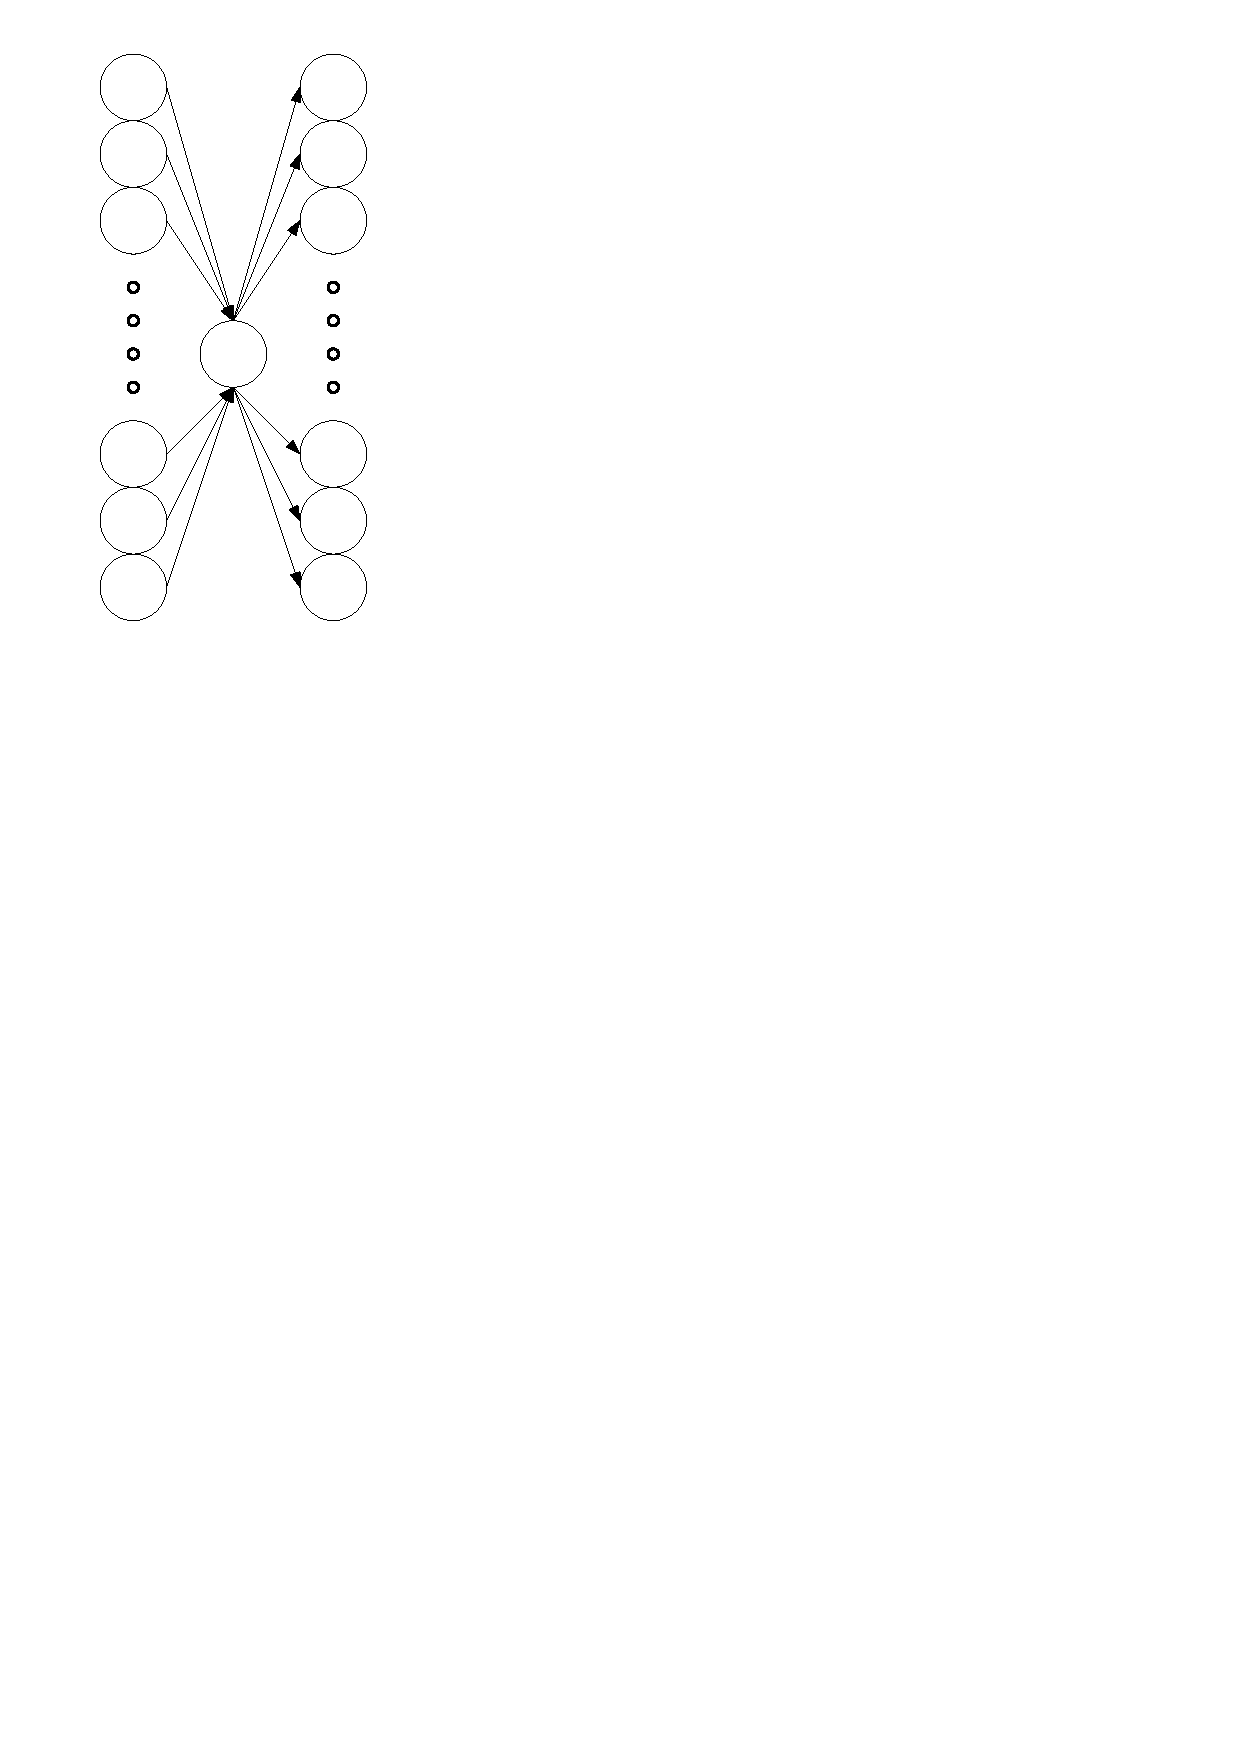
\includegraphics[scale=1.2]{bowtie.pdf}
   \end{center}
   Label the center vertex first, then the $m$ left vertices and finally the $n$
 right vertices, then the adjacency matrix of the bow tie graph becomes:
 
 $$B =\(
\left(
\begin{array}{c|ccc|ccc}
0       & 0 & \ldots & 0  & 1 & \ldots & 1\\\hline 
1 &  &             &     &    &              & \\
\vdots & & 0_{n\times n} & && 0_{n \times m}&\\
1 &  &             &     &    &              & \\ \hline
0 &  &             &     &    &              & \\
\vdots & & 0_{m \times n} & && 0_{m \times m}&\\
0 & & &     &    &              & \\


\end{array}
\right)
\) $$
 By direct computation, we get that the matrix $B^TB + BB^T$ is equal to:
 $$B^TB + BB^T = \begin{pmatrix}
 m + n & 0 & 0\\
 0 & 1_{n \times n} & 0\\
 0 & 0 & 1_{m \times m}
 \end{pmatrix}$$
 By Theorem \ref{centralescore}, the Perron root of $M$ is equal to $\rho = \sqrt{n+m}$ 
 because the central matrix $B^TB + B B^T$ has a dominant root $\rho^2$ of 
 $M^2$ and we clearly see that if we would take the characteristic polynomial of 
 $B^TB + BB^T$, we would get $m+n$ as Perron root. The dominant eigenvector of $B^TB + BB^T$ is equal
 to the similarity score $\mathbf{s}_2$ by Theorem \ref{centralescore}. it is now easy to see that:
 $$\mathbf{s}_2 = \left(\begin{array}{c}
 1 \\ \hline
 \mathbf{0}_{n}\\ \hline
 \mathbf{0}_{m}
\end{array}\right) $$
 If we see vertex 2 of the path graph $1 \to 2 \to 3$ as the \emph{center}\index{center}, 
 which can be seen as a vertex through which much information is passed, 
 then it is not surprising that $\mathbf{s}_2$ indicates that vertex $1$ of the directed 
 bow tie graph is the only one that looks like a center. The left vertices of 
 the bow tie graph look like vertex 1 of the path graph and the right vertices 
 of the bow tie graph look like vertex $3$. This is a beautiful example because 
 it confirms our intuition.
 \end{example}
 \subsubsection{Self-similarity of a graph}
When we compute the similarity matrix of two equal graphs $\graf = \grafeen$, 
the similarity matrix $S$ is  square matrix with as entries the similarity 
scores between vertices of $\graf$, we call $S$ the \emph{self-similarity matrix of $\graf$} 
\index{self-similarity}
in this case. 

Intuitively, we expect that vertices have the highest similarity scores with 
themselves, which means that the largest entries are located on the diagonal of 
$S$. We prove in the next theorem that the largest entry of a self-similarity 
matrix always appears on the diagonal and that, except for some special cases, 
the diagonal elements of a self-similarity matrix are nonzero. This doesn't mean
that the diagonal elements are always larger than the other elements on the same 
row or column and we conclude this paragraph with some easy examples the show 
this.

That the similarity matrix of a graph with itself is not always diagonally dominant is a serious limitation
on the intuitive concept of similarity between graphs! It shows that the 
algorithm is sometimes not capable to detect the essential link between a vertex and itself, which is one of 
the reasons why the presented algorithm of similarity is still not totally 
satisfactory.

To prove these statements, we first need to dive a little bit in the world of the 
symmetric, positive semidifinite matrices with some definitions and some proofs.

\begin{definition}\index{minor}\index{principal minor}\index{matrix!minor}\index{matrix!principal minor}
  Let $A$ be an $n \times n$-matrix, the determinant of a $k \times k$ principal submatrix (see Definition \ref{principalsubmatrix}) 
  is called a \textbf{principal minor of order k}.
\end{definition}

\begin{definition}\index{positive semidefinite matrix}\index{matrix!positive semidefinite matrix}
  A $n\times n$, symmetric matrix $A$ is called \textbf{positive semidefinite} if
all eigenvalues of $A$ are nonnegative.
\end{definition}
\begin{theorem}
  For a $n \times n$, symmetric matrix $A$, the following properties are equivalent:
  \begin{enumerate}
    \item $A$ is positive semidefinite,
    \item $A = U^T U$ for some matrix $U$,
    \item $\mathbf{x}^T A \mathbf{x} \geq 0$ for every $\mathbf{x} \in \R^n$,
    \item All principal minors $A$ are nonnegative.
  \end{enumerate}
\end{theorem}
\begin{proof}
  $(1)\Rightarrow (2)$ Write $A = UDU^T$ by Theorem \ref{diagonaal} where $U$ is 
  orthogonal and $D$ diagonal. Now, we know from that theorem, that the entries 
  on the diagonal of $D$ are the eigenvalues of $A$ (which are nonnegative), so 
  we may write $D = C^2$ where $C$ will also be a diagonal matrix. Then we have 
  $$A = UCCU^T = UC(UC)^T,$$
  as desired.
  
 $(2)\Rightarrow (3)$ For every $\mathbf{x} \in \R^n$ we have 
  $$\mathbf{x}^T A \mathbf{x} = \mathbf{x}^T U^T U \mathbf{x} = (U\mathbf{x})^T(U\mathbf{x}) 
  \geq 0.$$
 $(3)\Rightarrow (1)$ If $\mathbf{v}$ is an eigenvector of $A$ with eigenvalue $\lambda$ 
  then $0 \leq \mathbf{v}^T A \mathbf{v} = \lambda \mathbf{v}^T \mathbf{v}$ 
  which implies that $\lambda \geq 0$.
  
  $(2) \Rightarrow (4)$ Let $B$ be a submatrix of $A$ formed by deleting the rows 
  and columns with indices in the set $S$. Then modify $U$ to form $V$ by 
  deleting the columns with indices in the set $S$. Now: $\det(B) = \det(V^TV) = \det(V)^2 \geq 
  0$. Remember that $U$ is orthogonal from and thus $V$ is orthogonal too.
  
  $(4) \Rightarrow (1)$ By contraposition, we may assume that $A$ has a unit 
  eigenvector $\mathbf{v}$ with eigenvalue $\lambda \leq 0$. If $A$ has only one 
  eigenvalue $\leq 0$, then $\det(A) < 0$ and we are done. Otherwise, choose a 
  unit eigenvector $\mathbf{u}$ orthogonal to $\mathbf{v}$ with eigenvalue $\mu \leq 
  0$. Now choose $\alpha \in \R$ so that the vector $\mathbf{w} = \mathbf{v} + \alpha \mathbf{u}$ 
  has at least one zero coordinate, say $w_i$. If $A'$ is the matrix obtained 
  from $A$ by removing the column $i$ and row $i$ and $\mathbf{w'}$ is obtained 
  by removing coordinate $i$ of $\mathbf{w}$, then we have 
  $$(\mathbf{w'})^T A' \mathbf{w}' = \mathbf{w}^T A \mathbf{w} = \lambda + \alpha^2 \mu < 
  0, $$
  so $A'$ is not semidefinite since we already demonstrated the equivalence 
  between (3) and (1), and the result follows by induction.
 \end{proof}
\begin{lemma}
  The scaled sum of two positive semidefinite matrix is again a positive semidefinite matrix.
\end{lemma}
\begin{proof}
  Assume that $A$ and $B$ are $n\times n$, positive semidefinite matrices and $\alpha, \beta \in \R^{+}$, so for all $\mathbf{x} \in 
  \R^n$ we have $\mathbf{x}^T A \mathbf{x} \leq 0$, so then:
  $$\mathbf{x}^T (\alpha A + \beta B) \mathbf{x} = \alpha (\mathbf{x}^T  A  \mathbf{x}) + \beta (\mathbf{x}^T B \mathbf{x}) 
  \geq 0.$$
\end{proof}
\begin{theorem}
  The self-similarity matrix of a graph $\graf$ is positive semidefinite. The largest entry of the matrix appears on the 
diagonal and if a diagonal entry is equal to zero,  all the entries of the corresponding row and 
column are also equal to zero.
\end{theorem}
\begin{proof}
  Since $A = B$, the compact form of Theorem \ref{frobvorm} becomes:
 $$S^{(k+1)} = \frac{AS^{(k)}A^T + A^TS^{(k)}A}{\|AS^{(k)}A^T + A^TS^{(k)}A\|_F}, \quad S^{(0)} = J,  $$
  First notice that $S^{(k+1)}$ is in this case always symmetric because $s_{ij} = s_{ji}$ (the similarity scores of vertex $v_i$ and $v_j$
  are the same as the similarity scores of vertex $v_j$ and $v_i$). The all-one matrix $J$ is clearly 
  positive semidefinite
  as it has only nonnegative principal minors. So $S^{(0)}$ is postive semidefinite, so it can be decomposed as 
  $S^{(0)} = W^T W$. We write for some vector $\mathbf{x} \in \R^n$:
  \begin{eqnarray*}
    \mathbf{x}^T A^T S^{(0)} A \mathbf{x} &=&  \mathbf{x}^T A^T W^T W A \mathbf{x}\\
    &=& \|W A \mathbf{x}\|_2\\
    & \geq & 0,
  \end{eqnarray*}  
  similarly, $\mathbf{x}^T A S^{(0)} A^T \mathbf{x} \geq 0$, thus all matrices $S^{(k)}$ 
  are positive semidefinite because the (scaled) sum of two positive 
  semidefinite matrices is also positive semidefinite. Now, the rest of the 
  proof follows from the following observation: let $\alpha$ be a real number. If 
  $\mathbf{x} = \alpha e_i - e_j$ then:
  \begin{eqnarray}\mathbf{x}^t S^{(k)} \mathbf{x} = \alpha^2 s^{(k)}_{ii} - 2\alpha s^{(k)}_{ij} 
  +  s^{(k)}_{jj}\label{japan},
  \end{eqnarray}
  so to prove that the largest entry of the matrix $S^{(k)}$ appears on the 
  diagonal, assume, contrapositively, that the strictly largest entry is $s^{(k)}_{ij} = s^{(k)}_{ji}$ with $i \not = j$. Taking 
  $\alpha = 1$, equation (\ref{japan}) becomes:
  $$\mathbf{x}^t S^{(k)} \mathbf{x} =  s^{(k)}_{ii} - 2 s^{(k)}_{ij} 
  +  s^{(k)}_{jj} = (s^{(k)}_{ii} - s^{(k)}_{ij}) + (s^{(k)}_{jj} - s^{(k)}_{ij}) 
  < 0.$$
  To prove the last statement,  if $s^{(k)}_{ii} = 0$ but $s^{(k)}_{ij} \not = 
  0$ for some $j$ gives for (\ref{japan}):
  $$\mathbf{x}^t S^{(k)} \mathbf{x} = - 2\alpha s^{(k)}_{ij} 
  +  s^{(k)}_{jj},$$
which is negative for $\alpha$ large enough. 
  
\end{proof}
\begin{example}
  The self-similaritiy matrix of the graph:
  \begin{center}
  \begin{tikzpicture}[->,>=stealth',shorten >=1pt,auto,node distance=3cm,
                    thick]
                    \tikzstyle{every node}=[draw,circle,fill=black,minimum size=4pt,
                            inner sep=0pt]


  \node[main node] (1) [label=above:$v_1$] {};
  \node[main node] (2) [label=above:$v_2$][right of=1] {};
  \node[main node] (3) [label=above:$v_3$][right of=2] {};;

  \path[every node/.style={font=\sffamily\small}]
   
    (1) edge node [left] {} (2)
      (2) edge node [left] {} (3)
    
\end{tikzpicture}
\end{center}
is equal to:
$$\begin{pmatrix}
  0.5774 & 0 & 0 \\
  0 & 0.5774 & 0 \\
  0 & 0 & 0.5774
\end{pmatrix}$$
\end{example}

\begin{example}
  The self-similartiy matrix of the graph:
  \begin{center}
  \begin{tikzpicture}[->,>=stealth',shorten >=1pt,auto,node distance=3cm,
                    thick]
                    \tikzstyle{every node}=[draw,circle,fill=black,minimum size=4pt,
                            inner sep=0pt]


  \node[main node] (1) [label=above:$v_1$] {};
  \node[main node] (2) [label=left:$v_2$][below left of=1] {};
    \node[main node] (4) [label=right:$v_4$][below right of=1] {};

  \node[main node] (3) [label=below:$v_3$][below right of=2] {};;

  \path[every node/.style={font=\sffamily\small}]
   
    (1) edge node [left] {} (2)
      (2) edge node [left] {} (3)
      (3) edge node [left] {} (4)
      (4) edge node [left] {} (1)
    
\end{tikzpicture}
\end{center}
is equal to:
$$\begin{pmatrix}
  0.250 & 0.250 & 0.250 & 0.250 \\
  0.250 & 0.250 & 0.250 & 0.250 \\
  0.250 & 0.250 & 0.250 & 0.250 \\
  0.250 & 0.250 & 0.250 & 0.250 \\
\end{pmatrix}$$


\end{example}
\begin{example}
  The self-similartiy matrix of the graph:
  \begin{center}
  \begin{tikzpicture}[->,>=stealth',shorten >=1pt,auto,node distance=3cm,
                    thick]
                    \tikzstyle{every node}=[draw,circle,fill=black,minimum size=4pt,
                            inner sep=0pt]


  \node[main node] (1) [label=above:$v_1$] {};
  \node[main node] (2) [label=below:$v_2$][below of=1] {};
    \node[main node] (4) [label=right:$v_4$][below right of=2] {};

  \node[main node] (3) [label=left:$v_3$][below left of=2] {};;

  \path[every node/.style={font=\sffamily\small}]
   
    (1) edge node [left] {} (2)
      (2) edge node [left] {} (3)
      (2) edge node [left] {} (4)
    
\end{tikzpicture}
\end{center}
is equal to:
$$\begin{pmatrix}
  0.4082 & 0 & 0 & 0\\
  0 & 0.4082 & 0 & 0\\
  0 & 0 & 0.4082 & 0.4082\\
    0 & 0 & 0.4082 & 0.4082\\

\end{pmatrix}$$


\end{example}

\subsubsection{Undirected graphs}
In the case of undirected graphs, the compact form \ref{frobvorm} only 
becomes easier and equals:
\begin{theorem}
    Let $\graf$ and $\grafeen$ be two undirected graphs with adjacency matrices $A = [a_{ij}] \in \R^{n\times n}$ 
  and $B = [b_{ij}] \in \R^{m\times m}$ and let $S^{(0)} > 0$ be an initial positive matrix, and 
  define:

  $$S^{(k+1)} = \frac{BS^{(k)}A}{\|BS^{(k)}A\|_F}, \quad k = 
  0,1,\ldots.$$
  Then the matrix subsequences $S^{(2k)}$ and $S^{(2k+1)}$ converge to $S_\text{even}$ 
  and $S_\text{odd}$ and among all the matrices in the set of all possible 
  limits:
  $$\{S_\text{even}(S^{(0)}), S_\text{odd}(S^{(0)}): S^{(0)} > 0 \}$$
  the matrix $S_\text{even}(J)$ is the unique matrix of largest 
  1-norm.

\end{theorem}
\begin{proof}
  This follows easily from the fact that in the case of undirected graphs, $A$ 
  and $B$ are symmetric:
  \begin{eqnarray*}
     S^{(k+1)} &=& \frac{BS^{(k)}A^T + B^TS^{(k)}A}{\|BS^{(k)}A^T + 
     B^TS^{(k)}A\|_F}\\
     &=& \frac{BS^{(k)}A + BS^{(k)}A}{\|BS^{(k)}A + BS^{(k)}A\|_F}\\
     &=& \frac{2BS^{(k)}A}{\|2BS^{(k)}A\|_F}\\
     &=& \frac{BS^{(k)}A}{\|BS^{(k)}A\|_F}
\end{eqnarray*}
  
\end{proof}
\newpage
\section{Node-edge similarity}\index{node-edge similarity}
The paper of Blondel et al. \cite{blondel} caused a flow of successive papers 
which build upon the concept of similarity between two graphs. For instance, the paper
`Graph similarity scoring and 
matching' of Laura Zager and George Verghese \cite{zager} expands the 
notion of node similarity presented in the previous section to similarity 
between the edges of two graphs. The paper was presented in 2006. Intuitively an 
edge of a graph $\graf$ is similar to an edge of graph $\grafeen$ if their 
\emph{source} and \emph{terminal nodes} (Definition \ref{terminal}) are similar. As a consequence, the notion of similarity between edges
introduces a coupling between edge and node similarity scores. The algorithm presented in 
this paper is therefore an extension of the algorithm presented in the previous section.

\subsection{Coupled node-edge similarity scores}
We now present the extended algorithm allowing us to calculate not only a node 
similarity scores, but also edge similarity scores. The algorithm will use a 
new sort of matrices that represent a graph.  

\begin{definition}\index{source-edge matrix}\index{matrix!source-edge matrix}
  Let be $\graf=(V,\to)$ be a graph with adjacency matrix A, numbered vertices $v_1, v_2, \ldots, v_n \in V$ 
  and numbered edges $e_1, e_2, \ldots e_m  \in \to$. We define the \textbf{source-edge matrix $A_S$} as a $n\times m$ matrix with entries:
  $$(A_S)_{ij} = \begin{cases} 1 &\mbox{if }s_\graf(e_j) = v_i   \\ 
0 & \mbox{otherwise} \end{cases},$$
the notation $A_S$ is derived from the adjacency matrix $A$.
  \end{definition}
  
  \begin{definition}\index{terminal-edge matrix}\index{matrix!terminal-edge matrix}
  Let be $\graf=(V,\to)$ be a graph with adjacency matrix $A$, numbered vertices $v_1, v_2, \ldots, v_n \in V$ 
  and numbered edges $e_1, e_2, \ldots e_m  \in \to$. We define the \textbf{terminus-edge matrix $A_T$} as a $n\times m$ matrix with entries:
  $$(A_T)_{ij} = \begin{cases} 1 &\mbox{if }$t_\graf(e_j) = v_i$   \\ 
0 & \mbox{otherwise} \end{cases},$$
the notation $A_T$ is derived from the adjacency matrix $A$.  \end{definition}
\begin{property}\label{outdegreeprop}
Let $\graf=(V,\to)$ be a graph, then $A_SA^T_S$ is a diagonal matrix where the $i$th diagonal entry is equal the outdegree of vertex $v_i$.
   \end{property}
   \begin{proof}
By direct computation, we get:
$$(A_SA_S^T)_{ij} = \sum^m_{k=1}(A_S)_{ik}(A_S)^T_{kj} = \sum^m_{k=1}(A_S)_{ik}(A_S)_{jk}$$
Assume $i \not = j$. Then for each $k$, $(A_S)_{ik}(A_S)_{jk}= 0$ since vetrex $v_i$ 
and vertex $v_j$ can't be both the source node of edge $k$.

When $i=j$, then for each $k$, $(A_S)_{ik}(A_S)_{jk}= ((A_S)_{ik})^2$ equals 0 or 1 depending on whether $v_i$ 
is a starting point or not, so 1 is added to $(A_SA_S^T)_{ii}$ each time an edge `departs' from 
$v_i$, this is exactly the outdegree of vertex $v_i$.
   \end{proof}
   
In an analogous way, we prove:
\begin{property}\label{indegreeprop}
Let $\graf=(V,\to)$ be a graph, then $A_TA_T^T$ is a diagonal matrix where the $i$th diagonal entry is equal the indegree of vertex $v_i$.
   \end{property}

\begin{property}\label{adjacencyprop}
  Let $\graf =(V,\to)$ be a graph, then the adjacency matrix $A$ is equal to 
  $A_SA^T_T$.
\end{property}
\begin{proof}
  By direct computation, we get:
  $$(A_SA_T^T)_{ij} = \sum^m_{k=1}(A_S)_{ik}(A_T)^T_{kj} = \sum^m_{k=1}(A_S)_{ik}(A_T)_{jk}$$
The terms $(A_S)_{ik}(A_T)_{jk}$ equal $1$ if edge $k$ goes from $v_i$ to 
$v_j$ and since the sum is taken over all edges we conclude:
$$(A_SA_T^T)_{ij} = A_{ij}.$$
\end{proof}
Let  $\graf(V,\to)$, $\grafeen(U,\to')$ be two (directed) graphs, $\graf$ has $n_\graf$ vertices and $m_\graf$ edges and $\grafeen$ has $n_\grafeen$ vertices and $m_\grafeen$. 
Remember the following updating equation from (\ref{vergblondel}), which returns the 
(node) similarity score between vertices $u_i$ 
from $\grafeen$ and $v_j$ from $\graf$:
\begin{eqnarray*}
 x^{(k+1)}_{ij} = \sum_{r:(u_r,u_i)\in \to', w:(v_w,v_j) \in \to} x^{(k)}_{rw} +  \sum_{r:(u_i,u_r)\in \to', w:(v_j,v_w) \in \to} 
 x^{(k)}_{rw},
 \end{eqnarray*} 
if we number the edges of $\graf$ and $\grafeen$ as  $e_1, e_2, \ldots e_{m_\graf}  \in \to$ and $e'_1, e'_2, \ldots, e'_{m_\grafeen}  \in \to'$, this can be rewritten as:
 \begin{eqnarray*}
 x^{(k+1)}_{ij} = \sum_{t_\grafeen(e'_p)=u_i, t_\graf(e_q)=v_j} x^{(k)}_{s_\grafeen(e'_p)s_\graf(e_q)} +  \sum_{s_\grafeen(e'_p)=u_i, s_\graf(e_q)=v_j} 
 x^{(k)}_{t_\grafeen(e'_p)t_\graf(e_q)}.
 \end{eqnarray*} 
 We now extend this mutually reinforcing relation with the notion of edge 
 similarity. $x_{ij}$ denotes again the node similarity score between vertex $u_i$ from $\grafeen$ and vertex $v_j$ from $\graf$ 
 and $y_{pq}$ denotes the edge similarity score between edge $p$ from $\grafeen$ and edge $q$ in $\graf$, the update equations for edge and node similarity scores take now the 
 following form:
 \begin{eqnarray}
 y_{pq}^{(k+1)} &=& x^{(k)}_{s_\grafeen(e'_p)s_\graf(e_q)} + x^{(k)}_{t_\grafeen(e'_p)t_\graf(e_q)}\label{edge1}\\
 x^{(k+1)}_{ij} &=& \sum_{t_\grafeen(e'_r)=u_i, t_\graf(e_w)=v_j} y^{(k)}_{rw} +  \sum_{s_\grafeen(e_t)=u_i, s_\graf(e_w)=v_j} y^{(k)}_{rw} \label{edge2}
 \end{eqnarray} 
With the same 
 reasoning as presented in the previous section, these scores can be assembled into matrices $Y^{(k)}$ and $X^{(k)}$ 
by using the source-edge matrices $A_S$ and the terminus-edge matrices $A_T$. Let $A$ be the adjacency matrix of $\graf$ and $B$ be the adjacency
matrix of $\grafeen$, let $X^{(k)}$ be the $n_\grafeen \times n_\graf$-matrix with entries $x_{ij}$, the node similarity scores at iteration step $k$ 
and let $Y^{(k)}$ be the $m_\grafeen \times m_\graf$-matrix with entries $y_{pq}$, the edge similarity scores at step $k$. The equations (\ref{edge1}) and (\ref{edge2}) 
can be rewritten as:
\begin{eqnarray}
  Y'^{(k+1)} &=& B_S^TX^{(k)}A_S + B_T^TX^{(k)}A_T\label{edgematrix1}\\
   X'^{(k+1)} &=& B_SY^{(k)}A_S^T + B_TY^{(k)}A^T_T\label{edgematrix2}
 \end{eqnarray}
 for  $k =  0,1,\ldots$
 
 Of course we want to customize these equations in a way that we can apply Theorem \ref{grootbewijs} to prove convergence. 
 This will be completely analogous to Theorem \ref{frobvorm}, but we can achieve a slightly better result: not only the even and odd iterates
 will converge, the iteration converges as a whole. Lastly, remember that one of the conditions of Theorem \ref{grootbewijs} is to 
 normalize the results at each iteration step. Therefore, the following theorem comes as no surprise:

 \begin{theorem}\label{edgegrootbewijs}
   Let $\graf$ and $\grafeen$ be two graphs with adjacency matrices $A$ and $B$, $\graf$ has $n_\graf$ vertices and
   $m_\graf$ edges and $\grafeen$ has $n_\grafeen$ vertices and $m_\grafeen$ edges, define: 


   
 \begin{eqnarray}
  Y^{(k+1)} &=& \frac{B_S^TX^{(k)}A_S + B_T^TX^{(k)}A_T}{\|B_S^TX^{(k)}A_S + 
  B_T^TX^{(k)}A_T\|_F}\label{edgegroot1}\\
   X^{(k+1)} &=& \frac{B_SY^{(k)}A_S^T + B_TY^{(k)}A^T_T}{\|B_SY^{(k)}A_S^T + 
   B'_TY^{(k)}A^T_T\|_F}\label{edgegroot2}
 \end{eqnarray}
  for  $k =  0,1,\ldots$.
  
  Then the matrix subsequences $X^{(2k)}$, $Y^{(2k)}$ and $X^{(k+1)}$, $Y^{(k+1)}$ 
  converge to $X_{\text{even}}$, $Y_{\text{even}}$ and $X_{\text{odd}}$, 
  $Y_{\text{odd}}$. If we take:
  \begin{eqnarray*}  X^{(0)} = J \in \R^{n_\grafeen \times n_\graf}\\
    Y^{(0)} = J \in \R^{m_\grafeen \times m_\graf}
  \end{eqnarray*}
 as initial matrices, then $X_{\text{even}}(J)=X_{\text{odd}}(J)$, $Y_{\text{even}}(J)= Y_{\text{odd}}(J)$ 
 are the unique matrices of largest 1-norm among all possible limits with positive 
 initial matices and the matrix sequence $X^{(k)}$, $Y^{(k)}$ converges has a 
 whole.
  \end{theorem}
  \begin{proof}
 By Theorem \ref{tensor} we can rewrite (\ref{edgematrix1}) as follows:
 \begin{eqnarray*}
         Y'^{(k+1)} &=& B_S^TX'^{(k)}A_S + B_T^TX'^{(k)}A_T\\
  \Leftrightarrow  \vect(Y'^{(k+1)}) &=& \vect(B_S^TX'^{(k)}A_S + 
  B_T^TX'^{(k)}A_T)\\
  \Leftrightarrow  \vect(Y'^{(k+1)}) &=& \vect(B_S^TX'^{(k)}A_S) + 
  \vect(B_T^TX'^{(k)}A_T)\\
  \Leftrightarrow \vect(Y'^{(k+1)}) &=& (A_S^T \otimes B_S^T)\vect(X'^{(k)}) + (A^T_T \otimes 
  B^T_T)\vect(X'^{(k)})\\
   \Leftrightarrow \vect(Y'^{(k+1)}) &=& (A_S^T \otimes B_S^T + A^T_T \otimes 
  B^T_T)\vect(X'^{(k)})
 \end{eqnarray*}
 Completely analogously we can also rewrite (\ref{edgematrix2}):
 $$\vect(X'^{(k+1)}) &=& (A_S \otimes B_S + A_T \otimes B_T)\vect(Y^{k}),$$
 define $\mathbf{y}^{(k)}=\vect(Y'^{(k+1)})$ and $\mathbf{x}^{(k)}= \vect(X'^{(k+1)})$, we get:
 \begin{eqnarray*}
   \mathbf{y}^{(k+1)} &=& (A_S^T \otimes B_S^T + A^T_T \otimes 
   B^T_T)\mathbf{x}^{(k)}\\
   \mathbf{x}^{(k+1)} &=& (A_S \otimes B_S + A_T \otimes B_T)\mathbf{y}^{(k)}
 \end{eqnarray*} 
 If we define $G = A_S^T \otimes B_S^T + A^T_T \otimes B^T_T$, then with Lemma \ref{hulptensor} and well known
 properties of transpose matrices:
 \begin{eqnarray*}
   G^T &=& (A_S^T \otimes B_S^T + A^T_T \otimes B^T_T)^T\\
   &=& ((A_S\otimes B_S)^T + (A_T \otimes B_T)^T)^T\\
   &=& ((A_S\otimes B_S)^T)^T +  ((A_T \otimes B_T)^T)^T\\
   &=& A_S\otimes B_S + A_T \otimes B_T
 \end{eqnarray*}
 So we get:
  \begin{eqnarray}
     \mathbf{y}^{(k+1)} &=& G\mathbf{x}^{(k)}\label{uitgeschrevenvectoren1}\\
     \mathbf{x}^{(k+1)} &=& G^T\mathbf{y}^{(k)}\label{uitgeschrevenvectoren2},
 \end{eqnarray}
$G$ is a $m_\graf m_\grafeen \times n_\graf n_\grafeen$-matrix, the previous expressions  can be concatenated to a single matrix update equation (we define matrix $M$ and $\mathbf{z}^{(k+1)}$):
 $$\mathbf{z}^{(k+1)} =\begin{pmatrix}
 \mathbf{x}\\
 \mathbf{y}
 \end{pmatrix}^{(k+1)} = \begin{pmatrix}
 0_{m_\graf \times m_\grafeen} & G^T\\
 G & 0_{n_\graf \times n_\grafeen} \\
 \end{pmatrix}
 \begin{pmatrix}
 \mathbf{x}\\
 \mathbf{y}
 \end{pmatrix}^{(k)}
 = M\mathbf{z}^{(k)},$$
$M$ is clearly nonnegative because $G$ and $G^T$ consists of sums of Kronecker products of $A_S, B_S, A_T$ and/or $B_T$, all matrices
 with entries equal to zero or one, $M$ is as a $(n_\graf n_\grafeen + m_\graf m_\grafeen)\times(n_\graf n_\grafeen + m_\graf m_\grafeen)$-matrix
 clearly symmetric, so the result follows immediately from Theorem \ref{grootbewijs}. 
The appearance of the Perron norm can be explained in the same way as in Theorem \ref{frobvorm}, note that we write $Y^{(k)}$ and $X^{(k)}$ 
for the normalized results at iteration step $k$. We still have to prove that 
odd and even iterates are the same and that $M$ has only positive eigenvalues, meaning that the sequence converges to $\frac{\Pi \mathbf{z}^{(0)}}{\|\Pi \mathbf{z}^{(0)}\|_2}$,
this can be done easily by expanding the matrix equation: 
$$\mathbf{x}^{(k)} = \begin{cases} 
(G^TG)^{\frac{k}{2}}\mathbf{x}^{(0)  &\mbox{k even }\\
 
(G^TG)^{\frac{k-1}{2}}G^T\mathbf{y}^{(0)&\mbox{k odd}
\end{cases} \quad \text{and} \quad
\mathbf{y}^{(k)} = \begin{cases} 
(GG^T)^{\frac{k}{2}}\mathbf{y}^{(0)  &\mbox{k even }\\
 
(GG^T)^{\frac{k-1}{2}}G\mathbf{x}^{(0)&\mbox{k odd}
\end{cases}
$$
The matrix $G$ is the sum of two matrices $(A_S^T \otimes B_S^T)$ and $(A^T_T \otimes 
B^T_T)$. Now, $A_S^T$ is a $m_\graf \times n_\graf$-matrix and has in each row a 
single `$1$'-entry, simply because an edge has at most one source node . The same holds for 
$B_S^T$. Therefore, taking the Kronecker product of those two matrices results in the matrix $A_S^T \otimes B_S^T$
which also has just a single `$1$' entry in each row. With the same reasoning, 
we conclude that also $A^T_T \otimes B^T_T$ has also just a single `$1$'-entry in each row. Taking 
the sum of $(A_S^T \otimes B_S^T)$ and $(A^T_T \otimes 
B^T_T)$ results thus in the matrix $G$ with exactly two $1$ entries in each row. If we now choose the initial conditions as 
$\mathbf{x}^{(0)} = \mathbf{1} \in \R^{n_\grafeen n_\graf}$ and $\mathbf{y}^{(0)} = 
\mathbf{1} \in \R^{m_\grafeen m_\graf}$, we conclude:
$$G\mathbf{x}^{(0)} = 2\mathbf{y}^{(0)},$$
we get:
\begin{eqnarray*}
\mathbf{x}^{(k)} &=& \begin{cases} 
(G^TG)^{\frac{k-2}{2}}G^TG\mathbf{x}^{(0)} = \frac{1}{2}(G^TG)^{\frac{k-2}{2}}G^T\mathbf{y}^{(0)} &\mbox{$k$ even }\\
(G^TG)^{\frac{k-1}{2}}G^T\mathbf{y}^{(0)}&\mbox{$k$ odd}
\end{cases}\\
\mathbf{y}^{(k)} &=& \begin{cases} 
(GG^T)^{\frac{k}{2}}\mathbf{y}^{(0)}  &\mbox{$k$ even }\\
(GG^T)^{\frac{k-1}{2}}G\mathbf{x}^{(0)} = (GG^T)^{\frac{k-1}{2}}\frac{1}{2}\mathbf{y}^{(0)}\;\;\;\;\;\;\;\;\;\;\;\;\;&\mbox{$k$ odd}
\end{cases}
\end{eqnarray*}
First, observe that the matrices $GG^T$ and $G^TG$ are besides being symmetric (for example, $(GG^T)^T = GG^T$) 
and nonnegative, are also positive semi-definite and thus have only nonnegative 
eigenvalues. Note that the factor $\frac{1}{2}$ that appears in the odd iterates 
will be eliminated by the normalization in each step. So in the limit as $k \to \infty$ 
, the even and odd iterates are the same.

 \end{proof}
 We now define $X_{\text{even}}(\mathbf{1})$ as the node similarity matrix and $Y_{\text{even}}(\mathbf{1})$ as the edge similarity 
 matrix.
 
 
 

  \subsection{Algorithm 6 and Algorithm 7}
  \begin{algorithm}[h!]
 \KwData{\\
 $A_S$:  the $n_\graf \times m_\graf$ source-edge matrix of a graph $\graf$\\
 $A_T$:  the $n_\graf \times m_\graf$ terminal-edge matrix of a graph $\graf$\\
 $B_S$: the $n_\grafeen \times m_\grafeen$ source-edge matrix of a graph $\graf$\\
 $B_T$: the $n_\grafeen \times m_\grafeen$ terminal-edge matrix of a graph $\graf$\\
   $\tol$: tolerance for the estimation error.\\}
 \KwResult{\\
 $X$: the node similarity matrix between $\graf$ and $\grafeen$\\
 $Y$: the edge similarity matrix between $\graf$ and $\grafeen$}
 \blankline
\SetKwFunction{powermethod}{node\_edge\_similarity\_matrix}
\SetKwFunction{hits}{hits}

\SetKwProg{myalg}{begin}{}{end}
\myalg{\powermethod{$A_S$,$A_T$, $B_S$,$B_T$,$\tol$}}{
$k = 1$ \;
$X^{(0)} = \mathbf{1}$ ($n_\grafeen\times n_\graf$-matrix with all entries equal to $1$)\;
$Y^{(0)} = \mathbf{1}$ ($m_\grafeen\times m_\graf$-matrix with all entries equal to $1$)\;
$\mu_X =  n_\grafeen\times n_\graf$-matrix with all entries equal to $\tol$\;
$\mu_Y =  m_\grafeen\times m_\graf$-matrix with all entries equal to $\tol$\;

\Repeat{$|X^{(k)} - X^{(k-1)}| < \mu_X$ and $|Y^{(k)} - Y^{(k-1)}| < \mu_Y$ }{
$Y^{(k)}=& \frac{B_S^TX^{(k-1)}A_S + B_T^TX^{(k-1)}A_T}{\|B_S^TX^{(k-1)}A_S + B_T^TX^{(k-1)}A_T\|_F}$\;
$X^{(k)} = \frac{B_SY^{(k)}A_S^T + B_TY^{(k)}A^T_T}{\|B_SY^{(k)}A_S^T + B'_TY^{(k)}A^T_T\|_F}$\;
$k = k + 1$\;
}
 
\KwRet $X^{(k)}, Y^{(k)} $\;}{}
  \caption{Algorithm for calculating the node and edge similarity matrix $X$ and $Y$ between $\graf$ and $\grafeen$.}\label{edgealgorithm}
\end{algorithm}
 
 The algorithm to calculate the node and edge similarity scores is presented in pseudo-code in Algorithm 6. 
 Remember that the absolute value that is mentioned is the same as in Notation 
 \ref{modulusmatrix}. Besides the different calculations, the main difference with the algorithm of the previous section (Algorithm \ref{algsimilarity})
 is that the whole sequence converges, not only the even (or odd) iterates, 
 making this algorithm twice as fast. This is because in Algorithm \ref{algsimilarity} we take the limit
 of the even iterates but we need the calculations of the odd iterates too to achieve a result. In this
 implementation, the algorithm will not oscillate and both the even and odd iterates converge to the same limit, so the tolerance level will
 be satisfied with half of the number of steps we would need for Algorithm \ref{algsimilarity}. Also notice that we implement a \textit{sequential} 
 update: when $Y^{(k)}$ is calculated,the result is immediately used in 
 $X^{(k)}$. This is not according to Theorem \ref{edgegrootbewijs}, which 
 suggest \textit{simultaneous} updating equations: in that case $X^{(k)}$ uses $Y^{(k-1)}$ 
 in its calculations. It is not difficult to see, by an analogous argument of 
 Theorem \ref{edgegrootbewijs}, that both approaches yield the same set of 
 similarity scores. Numerical analysts, however, will always prefer the sequential
 update procedure because it performs slightly better (see section 3.2 in \cite{numeriekewiskunde}) as you directly use a more accurate 
 result for $Y^{(k)}$ in the calculation of $X^{(k)}$. 
 
 A Matlab implementation 
 can be found in Listing \ref{edgematlab} in Appendix \ref{appendixa}. Because giving source-edge matrices and terminal-edge matrices as input
 is quite unnatural, in Listing \ref{sourceedgematlab} and Listing \ref{terminaledgematlab} 
 some Matlab code is also presented to transform an adjacency matrix into a 
 source-edge matrix and a terminal-edge matrix. The resulting matrices represent an edge numbering left-to-right, based on the entries of the adjacency matrix. The algorithm to calculate the 
 source-edge matrix based on the adjacency matrix is also written in pseudo-code in Algorithm 
 \ref{sourceedge}, the calculation of the terminal-edge matrix is completely 
 analogous. A Matlab implementation of Algorithm \ref{edgealgorithm} that takes 
 two adjacency matrices as input can be found in Listing \ref{zeeruitgebreid}.
 
   \begin{algorithm}[H]\label{sourcedge}
 \KwData{\\
 $A$:  the $n \times n$ adjacency matrix of a graph $\graf$\\
 \KwResult{\\
 $A_S$: the source-edge matrix of graph $\graf$}
 \blankline
\SetKwFunction{powermethod}{source\_edge\_matrix}
\SetKwFunction{hits}{hits}

\SetKwProg{myalg}{begin}{}{end}
\myalg{\powermethod{$A$}}{
$m$ = sum of all entries of $A$ \;
$A_S$ = initialize a $n \times m$-matrix with all entries equal to 0\;
current\_edge = 1\;

\For{$i: 1$ to $n$ }{
  \For{$j: 1$ to $n$ }{
     \If{$(A)_{ij} > 0$}{
          \For{$e: 1$ to $(A)_{ij}$}{
            $(A_S)_{i, \text{current\_edge }}$ = 1\;
            current\_edge = current\_edge + 1 \;
          }
     }
  }}}
 
\KwRet $A_S$\;}{}
  \caption{Algorithm for calculating the source-edge matrix $A_S$ based on the adjacency matrix $A$ of a graph $\graf$.\\}\label{sourceedge}
\end{algorithm}
 
 \subsection{Difference with node similarity}
It is clear that the node-edge similarity algorithm is different from 
Algorithm \ref{algsimilarity} from the previous section. We will make this a little 
more explicit and show the difference in the resulting node similarity matrix. We first need another property of the Kronecker 
product.

\begin{property}\textbf{(mixed-product property of Kronecker products)}
  Let $A \in \R^{m\times n}, B \in \R^{r \times s}, C \in \R^{n\times p}$ and $D \in \R^{s \times t}$ 
  then:
  $$(A\otimes B)(C \otimes D) = AC \otimes BD$$
\end{property}
\begin{proof}
  \begin{eqnarray*}
(A\otimes B)(C \otimes D) &=&
  \begin{pmatrix}
    a_{11}B & \ldots & a_{1n}B\\
    \vdots & \ddots & \vdots\\
    a_{m1}B & \ldots & a_{mn}B
  \end{pmatrix}
  \begin{pmatrix}
    c_{11}D & \ldots & c_{1p}D\\
    \vdots & \ddots & \vdots\\
    a_{n1}D & \ldots & a_{np}D
  \end{pmatrix}\\
  &=& \begin{pmatrix}
    \sum_{k=1}^n a_{1k}c_{k1}BD & \ldots & \sum_{k=1}^n a_{1k}c_{kp}BD\\
    \vdots & \ddots & \vdots\\
    \sum_{k=1}^n a_{mk}c_{k1}BD & \ldots & \sum_{k=1}^n a_{mk}c_{kp}BD\\
  \end{pmatrix}\\
  &=& AC \otimes BD.
  \end{eqnarray*}
\end{proof}



Now take equations (\ref{uitgeschrevenvectoren1}) and 
(\ref{uitgeschrevenvectoren2}) and consider only the even iterates. We consider only the even iterates because Algorithm \ref{algsimilarity} does, 
remember that in Algorithm \ref{edgealgorithm} the even and odd iterates yield 
the same set of similarity scores. We get:
\begin{eqnarray*}
  \mathbf{x}^{(k)} &=& (G^TG)\mathbf{x}^{(k-2)}\\
  &=& ((A_S\otimes B_S + A_T \otimes B_T)(A^T_S \otimes B^T_S + A^T_T \otimes 
  B^T_T))\mathbf{x}^{(k-2)}\\
  &=& ((A_S\otimes B_S)(A^T_S \otimes B^T_S) + (A_S\otimes B_S)(A^T_T \otimes 
  B^T_T) \\
  &\quad& + (A_T \otimes B_T)(A^T_S \otimes B^T_S) + (A_T \otimes B_T)(A^T_T \otimes 
  B^T_T))\mathbf{x}^{(k-2)}\\
  &=& (A_S A^T_S \otimes B_SB^T_S + A_SA^T_T \otimes B_SB^T_T \\
  &\quad& + A_TA^T_S \otimes 
  B_TB^T_S + A_TA^T_T\otimes B_TB^T_T)\mathbf{x}^{(k-2)}\\
  &=& (A_S A^T_S \otimes B_SB^T_S + A \otimes B + A^T \otimes B^T + A_TA^T_T\otimes 
  B_TB^T_T)\mathbf{x}^{(k-2)}\\
  &=& (A \otimes B + A^T \otimes B^T + A_S A^T_S \otimes B_SB^T_S + A_TA^T_T\otimes 
  B_TB^T_T)\mathbf{x}^{(k-2)}
\end{eqnarray*}
Where $A, B$ are the adjacency matrices of $\graf, \grafeen$ (Property 
\ref{adjacencyprop}), 
$A_S A^T_S, B_S B^T_S$ are the diagonal matrices with the outdegrees of the vertices 
on the diagonal (Property \ref{outdegreeprop}) and $A_TA^T_T, 
  B_TB^T_T$ are the diagonal matrices with the indegree of the vertices on the 
  diagonal (Property \ref{indegreeprop}). The iteration sugested in Theorem \ref{frobvorm} 
  in the previous section has the following form (see equation 
  (\ref{uitgeschrevenvectornormaal})):
  $$\mathbf{x}^{(k)} = A \otimes B + A^T \otimes B^T\mathbf{x}^{(k-2)},$$
thus Algorithm \ref{edgealgorithm} differs from Algorithm \ref{algsimilarity} in three important ways:
\begin{itemize}
  \item  In Algorithm \ref{edgealgorithm} the inclusion of additional diagonal terms serve to amplify the scores of 
nodes that are highly connected in the node similarity matrix,
\item  Algorithm \ref{edgealgorithm} returns a node similarity matrix and an edge similarity matrix, Algorithm \ref{algsimilarity}
returns only a node similarity matrix,
\item The whole sequence in Algorithm \ref{edgealgorithm} converges, not only 
the even and odd iterates.

\end{itemize}
  
  
 \subsection{Example}
 \begin{example}
   We retake Example \ref{eenvoudigvoorbeeldjes} and number the edges as 
   follows, let $\graf = (V,\to)$ be :
\begin{center}
\begin{tikzpicture}[->,>=stealth',shorten >=1pt,auto,node distance=3cm,
                    thick]
                    \tikzstyle{every node}=[draw,circle,fill=black,minimum size=4pt,
                            inner sep=0pt]


  \node[main node] (1) [label=above:$v_1$] {};
  \node[main node] (2) [label=above:$v_2$][right of=1] {};
  \node[main node] (3) [label=above:$v_3$][right of=2] {};;

  \path[every node/.style={font=\sffamily\small}]
   
    (1) edge node [above] {1} (2)
      (2) edge node [above] {2} (3)
    
\end{tikzpicture}
\end{center}
Let $\grafeen=(W,\to)$ be the following graph:
 \begin{center}
\begin{tikzpicture}[->,>=stealth',shorten >=1pt,auto,node distance=3cm,
                    thick]
                    \tikzstyle{every node}=[draw,circle,fill=black,minimum size=4pt,
                            inner sep=0pt]

 \node[main node] (1) [label=above:$w_1$] {};

  \node[main node] (2) [label=left:$w_2$] [below left of =1; left of=3]{};
  \node[main node] (3) [label=right:$w_3$][below right of=1;] {};
    \node[main node] (4) [label=left:$w_4$][below of=2] {};
  \node[main node] (5) [label=right:$w_5$][below of=3] {};
  \path[every node/.style={font=\sffamily\small}]
       (1) edge node [left] {$1$} (2)
      (1) edge node [right] {$2$} (3)
      (2) edge node [near start, below] {$5$} (5)
            (2) edge node [above] {$3$} (3)

      (2) edge node [left] {$4$} (4)
      (3) edge node [near start] {$6$} (4)
      (3) edge node [right] {$7$} (5)

\end{tikzpicture}
\end{center}
Then the node similarity matrix is:

$$X = \begin{pmatrix}
0.2338  &  0.0718  &       0\\
0.2472   & 0.3230  &  0.0128\\
0.1841   &  0.7553 &   0.3185\\
0  &  0.0935  &  0.2338\\
0   & 0.0441 &   0.0576
\end{pmatrix},$$
 and the edge similarity matrix equals:
 $$ Y = \begin{pmatrix}
0.2166 & 0.0329\\
0.3847 & 0.1518\\
0.3899 & 0.2495\\
0.1325 & 0.2166\\
0.1133 & 0.1480\\
0.3653 & 0.4176\\
0.1080 & 0.3847
\end{pmatrix}$$
If you look at the structure of $\grafeen$ and compare it with the structure of $\graf$, then 
intuitively it is not surprising that edge $3$ of $\grafeen$ is most similar to edge $1$ of 
$\graf$ and edge $6$ of $\grafeen$ is most similar to edge $2$ of $\graf$ because they are both very
central edges with source nodes and terminal nodes that are very similar (they both have high similarity scores). 
Also note that $w_7$ is considered as the most `central node' (see subsection \ref{centralescooores}) as it has the 
largest similarity score for $v_2$, also this can be explained because $w_3$ has 2 incoming edges and 2 outgoing
eges, no other edge has this in $\grafeen$. \end{example}
 


\section{Colored graphs}\index{colored graph}\index{graph!colored graph}
In this last section, we extend the notion of similarity to colored graphs. The 
paper \cite{vandoren} is written by two Belgian professors Paul Van Dooren and 
Catherine Fraikin from the Catholic University of 
Louvain in 2009.

Graph coloring is already introduced in paragraph \ref{colored} and we will 
construct a method that returns similarity matrices for two graphs where the coloring is on the nodes or 
on the edges of both graphs. If you would compare the original paper to 
explanation in this section, you will see that there are a lot of differences. 
This has two reasons: first, with the previous sections we have already a broad overview of 
similarity on graphs so we can achieve results in a more detailed way, second, to make 
the notations uniform in the whole master thesis, this paper had to be 
rewritten.


\subsection{Colored nodes}\index{node coloring}
\subsubsection{Method}
We first extend the node similarity introduced in section \ref{sectionnodesim} to 
node colored graphs. Take two node colored graphs $\graf=(V,\to, C, a)$ and $\grafeen=(U,\to', C, a')$ with $|C|$ (remember that $a$, $a'$ are surjective) different colors and assume that the nodes 
in both graphs are renumbered such that those of color $1$ come first, then 
those of color $2$,... The adjacency matrices $A$ (of graph $\graf$) and $B$ (of graph $\grafeen$) 
can then be partitioned as follows:
$$A = \begin{pmatrix}
A_{11} & A_{12} & \ldots & A_{1|C|}\\
A_{11} & A_{12} & \ldots & A_{1|C|}\\
\vdots & \vdots & \ddots & \vdots\\
A_{|C|1} & A_{|C|2} & \ldots & A_{|C||C|}\\
\end{pmatrix}
 \quad \text{and} \quad
 \begin{pmatrix}
B_{11} & B_{12} & \ldots & B_{1|C|}\\
B_{11} & B_{12} & \ldots & B_{1|C|}\\
\vdots & \vdots & \ddots & \vdots\\
B_{|C|1} & B_{|C|2} & \ldots & B_{|C||C|}\\
\end{pmatrix}$$
Remember that $c_\graf(V,i)$ denotes the number of vertices of color $i$ in graph $\graf$, then each block $A_{ij} \in \R^{c_\graf(V,i)\times c_\graf(V,j)}$ and $B_{ij} \in \R^{c_\grafeen(U,i)\times c_\grafeen(U,j)}$ 
describes the adjacency relations between the nodes of color $i$ to the vertices 
of color $j$ in both $A$ and $B$. In fact, by just renumbering the vertices such 
that the nodes with the same color succeed each other, you immediately get such 
partitioning. If you see this renumbering as a permutation on the nodes,
then performing on the original adjacency matrix a left and right multiplication with the corresponding permutation matrix (see Definition 
\ref{petmruation}) leads to this adjusted adjacency matrix.
To make the idea more comprehensible, we give an example.\index{partitioned adjacency matrix}

\begin{example}
  Let $\graf$ be following graph:
  \begin{center}
\begin{tikzpicture}[->,>=stealth',shorten >=1pt,auto,node distance=3cm,
                    thick]
                    \tikzstyle{every node}=[draw,circle,fill=black,minimum size=6pt,
                            inner sep=0pt]


  \node[main node, fill=green] (1) [label=below:$v_1$] {};
  \node[main node, fill=blue] (2) [label=below:$v_2$][right of=1] {};
  \node[main node, fill=green] (3) [label=below:$v_3$][right of=2] {};;
  \node[main node, fill=yellow] (4) [label=below:$v_4$][right of=3] {};;

  \path[every node/.style={font=\sffamily\small}]
   
    (1) edge node [above] {} (2)
    (1) edge[bend right=30]  node [below] {} (3)

    (2) edge node [above] {} (3)
     (3) edge node [above] {} (4)
     (3) edge [bend right=30] node [below] {} (4)
     (2) edge [bend left=40] node [above] {} (3)
     (3) edge [bend right=40] node [above] {} (2)
     (4) edge [loop above] node {} (4)
\end{tikzpicture}
\end{center}
The adjacency matrix equals:
$$A = \begin{pmatrix}
0 & 1 & 1  & 0\\
0 & 0 & 2 & 0\\
0 & 1 & 0 & 2\\
0 & 0 & 0 & 1\\
\end{pmatrix}.$$
If we order the colors as: $\{\text{green, blue, yellow}\}$ (so color 1 = green, color 2 = blue, color 3 = yellow), we can renumber the 
vertices and get the following graph:
\begin{center}
\begin{tikzpicture}[->,>=stealth',shorten >=1pt,auto,node distance=3cm,
                    thick]
                    \tikzstyle{every node}=[draw,circle,fill=black,minimum size=6pt,
                            inner sep=0pt]


  \node[main node, fill=green] (1) [label=below:$v_1$] {};
  \node[main node, fill=green] (2) [label=below:$v_2$][right of=1] {};
  \node[main node, fill=blue] (3) [label=below:$v_3$][right of=2] {};;
  \node[main node, fill=yellow] (4) [label=below:$v_4$][right of=3] {};;

  \path[every node/.style={font=\sffamily\small}]
    (1) edge[bend right=30] node [below] {} (3)
    (1) edge node [below] {} (2)

    (3) edge node [above] {} (2)
     (2) edge[bend right=30] node [below] {} (4)
     (2) edge[bend right=20] node [below] {} (4)
        (2) edge [bend left=40] node [above] {} (3)
     (3) edge [bend right=40] node [above] {} (2)
          (4) edge [loop above] node {} (4)

\end{tikzpicture}
\end{center}

The adjacency matrix equals:
$$A' = PAP = \begin{pmatrix}
1 & 0 & 0 & 0\\
0 & 0 & 1 & 0\\
0 & 1 & 0 & 0\\
0 & 0 & 0 & 1
\end{pmatrix}\begin{pmatrix}
0 & 1 & 1  & 0\\
0 & 0 & 2 & 0\\
0 & 1 & 0 & 2\\
0 & 0 & 0 & 1\\
\end{pmatrix}\begin{pmatrix}
1 & 0 & 0 & 0\\
0 & 0 & 1 & 0\\
0 & 1 & 0 & 0\\
0 & 0 & 0 & 1
\end{pmatrix}=
\begin{pmatrix}
0 & 1 & 1 & 0\\
0 & 0 & 1 & 2\\
0 & 2 & 0 & 0\\
0 & 0 & 0 & 1
\end{pmatrix},$$
which can be partitioned in blocks as follows (we have 3 colors: 1 = green, 2 = blue, 3 = yellow):
$$A' = \begin{pmatrix}
A_{11} & A_{12} & A_{13}\\
A_{21} & A_{22} & A_{23}\\
A_{31} & A_{32} & A_{33}\\
\end{pmatrix} =
\begin{pmatrix}\smallskip
\begin{pmatrix}
 0 & 1\\
 0 & 0\\
\end{pmatrix}& 
\begin{pmatrix}
 1\\
 1\\
\end{pmatrix}
& \begin{pmatrix}
0\\
2\\
\end{pmatrix}\\ \smallskip
 \begin{pmatrix}
0 & 2\\
\end{pmatrix} & \begin{pmatrix}
 0\\
\end{pmatrix} & \begin{pmatrix}
 0\\
\end{pmatrix}\\
\begin{pmatrix}
 0 & 0\\
\end{pmatrix} & \begin{pmatrix}
 0\\
\end{pmatrix} & \begin{pmatrix}
 1\\
\end{pmatrix}\\
\end{pmatrix} .$$
\end{example}
Now, we will only compare the nodes of the same color in both graphs, so that we 
define similarity matrices $S_{ii} \in \R^{c_\graf(V,i)\times c_\grafeen(v_i)}$, with 
$i=1,\ldots,|C|$, which we can put in a block-diagonal similarity matrix:
$$S = \begin{pmatrix}
S_{11} & 0 & \ldots & 0\\
0 & S_{12} & \ldots & 0\\
\vdots & \vdots & \ddots & \vdots\\
0 & 0 & \ldots & S_{|C||C|}
\end{pmatrix}$$



\begin{theorem}
  Let $\graf=(V,\to, C, a)$ and $\grafeen=(U,\to', C, a')$ be two node colored graphs and define:
  \begin{eqnarray*}
  Z^{(k+1)}_1 &=& \sum_{i \in \{1,\ldots, |C|\}}B_{1i}S^{(k)}_{ii}A^T_{1i} + B^T_{i1}S^{(k)}_{ii}A_{i1}\\
  Z^{(k+1)}_2 &=& \sum_{i \in \{1,\ldots, |C|\}}B_{2i}S^{(k)}_{ii}A^T_{2i} + B^T_{i2}S^{(k)}_{ii}A_{i2} \\
  &\vdots& \\
    Z^{(k+1)}_{|C|} &=& \sum_{i \in \{1,\ldots, |C|\}}B_{|C|i}S^{(k)}_{ii}A^T_{|C|i} + B^T_{i|C|}S^{(k)}_{ii}A_{i|C|} \\
 (S_{11}, S_{22},\ldots, S_{|C| |C|} )^{(k+1)} &=& \frac{\left(Z^{(k+1)}_1, Z^{(k+1)}_2, \ldots,Z^{(k+1)}_{|C|}\right)}{\left|\left|\left(Z^{(k+1)}_1, Z^{(k+1)}_2, \ldots,Z^{(k+1)}_{|C|}\right)\right|\right|_F}
  \end{eqnarray*}
 for $k = 0,1,\ldots$

 Then the the matrix subsequences $Z^{(2k)}_j$ for every $j \in \{1, \ldots, |C|\}$ 
 and $(S_{11}, S_{22},\ldots, S_{|C| |C|} )^{(2k)}$ converge to $Z^{\text{even}}_j$ and  $(S_{11}, S_{22},\ldots, S_{|C| |C|} 
 )^{\text{even}}$. Also the odd subsequences converge. If we take:
 $$S^{(0)}_{jj} = J\in \R^{c_\grafeen(U,j)\times c_\graf(V,j)}$$
 as initial matrices, then the resulting $S^{\text{even}}_{jj}(\mathbf{1})$ are 
 the unique matrices of largest 1-norm among all possible limits with positive 
 start vector.
  
\end{theorem}
  
\begin{proof}
   By induction on $|C|$. Remember from Definition \ref{defcolor} that the function $a$ is surjective, meaning that
  $C$ only consists of colors that are actually used.
    
   For $|C|=1$, we have a graph with all vertices having the same color, which can be seen as an uncolored graph. This is just 
   the normal case as proved in Theorem \ref{frobvorm}.
      
Although redundant, it is instructive to prove the case $|C|=2$ separately, because the 
generalization in the induction step is then immediately clear, so consider 
the partitioned adjacency matrices:
$$\begin{pmatrix}
A_{11} & A_{12}\\
A_{21} & A_{22}\\
\end{pmatrix} \quad \text{and} \quad
\begin{pmatrix}
B_{11} & B_{12}\\
B_{21} & B_{22}\\
\end{pmatrix},$$
the equations of the theorem are in this case:

\begin{eqnarray*}
  Z'^{(k+1)}_1 &=& B_{11}S^{(k)}_{11}A_{11}^T + B^T_{11}S^{(k)}_{11}A_{11} + B_{12}S^{(k)}_{22}A_{12}^T + B^T_{21}S^{(k)}_{22}A_{21}\\
  Z'^{(k+1)}_2 &=& B_{21}S^{(k)}_{11}A_{21}^T + B^T_{12}S^{(k)}_{11}A_{12} + B_{22}S^{(k)}_{22}A_{22}^T + B^T_{22}S^{(k)}_{22}A_{22} \\
 (S_{11}, S_{22})^{(k+1)} &=& \frac{(Z'^{(k+1)}_1, Z'^{(k+1)}_2)}{\|(Z'^{(k+1)}_1, Z'^{(k+1)}_2)\|_F}
 \end{eqnarray*}
We can write with Theorem \ref{tensor}:
\begin{eqnarray*}
  Z'^{(k+1)}_1 &=& B_{11}Z'^{(k)}_1A_{11}^T + B^T_{11}Z'^{(k)}_1A_{11} + B_{12}Z'^{(k)}_2A_{12}^T + B^T_{21}Z'^{(k)}_{2}A_{21}\\
 \Leftrightarrow \vect(Z'^{(k+1)}_1) &=& \vect(B_{11}Z'^{(k)}_1A_{11}^T + B^T_{11}Z'^{(k)}_1A_{11} + B_{12}Z'^{(k)}_2A_{12}^T + B^T_{21}Z'^{(k)}_{2}A_{21})\\
  \Leftrightarrow \vect(Z'^{(k+1)}_1) &=& (A_{11}\otimes B_{11})\vect{Z'^{(k)}_1}  
  + (A^T_{11}\otimes B^T_{11})\vect(Z'^{(k)}_1) \\
  && \;\; + (A_{12}\otimes B_{12})\vect(Z'^{(k)}_2)
  + (A^T_{21}\otimes B^T_{21})\vect(Z'^{(k)}_2) \\
  \Leftrightarrow \vect(Z'^{(k+1)}_1) &=& (A_{11}\otimes B_{11} + A^T_{11}\otimes B^T_{11})\vect(Z'^{(k)}_1)  \\ 
&&  \;\; + (A_{12}\otimes B_{12}+A^T_{21}\otimes B^T_{21})\vect(Z'^{(k)}_2)
 \end{eqnarray*}
 In a similar way, we can write $Z'^{(k+1)}_2$, which is the not normalized version of $Z^{(k+1)}_2$, as:
 \begin{eqnarray*}
 \vect(Z'^{(k+1)}_2) &=& (A_{21}\otimes B_{21} + A^T_{12}\otimes B^T_{12})\vect{Z'^{(k)}_1} + (A_{22}\otimes B_{22}+A^T_{22}\otimes B^T_{22})\vect{Z'^{(k)}_2}\\
\end{eqnarray*}
If we define $M$, $\mathbf{z}^{k+1}$ as follows, the previous expressions 
concatenate to a single matrix update equation:
\begin{eqnarray*}
\mathbf{z}^{(k+1)} &=& \begin{pmatrix}
\vect(Z'_1)\\
\vect(Z'_2)\\
\end{pmatrix}^{(k+1)}\\
&=& \begin{pmatrix}
A_{11}\otimes B_{11} + A^T_{11}\otimes B^T_{11}& A_{12}\otimes B_{12}+A^T_{21}\otimes B^T_{21}\\
A_{21}\otimes B_{21} + A^T_{12}\otimes B^T_{12} & A_{22}\otimes B_{22} + A^T_{22}\otimes B^T_{22}
\end{pmatrix}
\begin{pmatrix}
\vect(Z'_1)\\
\vect(Z'_2)\\
\end{pmatrix}^{(k)}\\
&=& M\mathbf{z}^{(k)}
\end{eqnarray*}
Notice that the diagonal blocks in $M$ are related to links between the nodes with the same color, 
while the off diagonal blocks refer to links between nodes of another color. As 
always, we want to use Theorem \ref{grootbewijs} to get the result. $M$ is 
clearly nonnegative, because every block $A_{ij}$ and $B_{ij}$ is nonnegative (it is derived from the nonnegative adjacency matrices $A$ and 
$B$). Proving that $M$ is symmetric a bit trickier, but notice that $A_{11}\otimes B_{11} + (A_{11}\otimes B_{11})^T$
is a symmetric $c_\graf(1)c_\grafeen(1)\times c_\graf(1)c_\grafeen(1)$ matrix (because it is the sum of a matrix with his transpose), and $A_{22}\otimes B_{22} + (A_{22}\otimes B_{22})^T$ is a symmetric 
$c_\graf(2)c_\grafeen(2)\times c_\graf(2)c_\grafeen(2)$. If we define $G = A_{21} \otimes B_{21} + A^T_{12}\otimes B^T_{12}$, $G$ is a $c_\graf(2)c_\grafeen(2) \times c_\graf(1)c_\grafeen(1)$-matrix. Now, notice the following relation between the off diagonal blocks:
\begin{eqnarray*}
  G^T &=& (A_{21} \otimes B_{21} + A^T_{12}\otimes B^T_{12})^T \\
  &=& (A_{21} \otimes B_{21})^T + ((A^T_{12}\otimes B^T_{12})^T)^T\\
  &=& A_{12}\otimes B_{12}+A^T_{21}\otimes B^T_{21}
  \end{eqnarray*}
$G^T$ is a $c_\graf(1)c_\grafeen(1) \times c_\graf(2)c_\grafeen(2)$-matrix.
So we can rewrite $M$ as:
$$M = \begin{pmatrix}
A_{11}\otimes B_{11} + A^T_{11}\otimes B^T_{11}& G^T\\
G & A_{22}\otimes B_{22} + A^T_{22}\otimes B^T_{22}
\end{pmatrix}$$
 $M$ is a $(c_\graf(1)c_\grafeen(1)+c_\graf(2)c_\grafeen(2))\times(c_\graf(1)c_\grafeen(1)+c_\graf(2)c_\grafeen(2))$-matrix, we want to prove that $(M)_{ij}  = (M)_{ji}$ and to do so we distinguish all possible cases: 
 
\begin{itemize}
  \item If $i \leq c_\graf(1)c_\grafeen(1), j \leq c_\graf(1)c_\grafeen(1)$, 
  then $(M)_{ij}$ and $(M)_{ji}$ will both be entries of $A_{11}\otimes B_{11} + A^T_{11}\otimes B^T_{11}$ and this submatrix was symmetric.
  \item If $i \leq c_\graf(1)c_\grafeen(1), j > c_\graf(1)c_\grafeen(1)$, then $(M)_{ij}$ 
  will be an entry of $G^T$ and $(M)_{ji}$ will be an entry of $G$, so they are 
  equal.
  \item If $i > c_\graf(1)c_\grafeen(1), j > c_\graf(1)c_\grafeen(1)$, then $(M)_{ij}$ and $(M)_{ji}$ will both be entries of $A_{22}\otimes B_{22} + A^T_{22}\otimes B^T_{22}$ and this submatrix was symmetric.
   \item If $i > c_\graf(1)c_\grafeen(1), j \leq c_\graf(1)c_\grafeen(1)$, then $(M)_{ij}$ 
  will be an entry of $G$ and $(M)_{ji}$ will be an entry of $G^T$, so they are 
  equal.
  \end{itemize}

The result immediately follows from Theorem \ref{grootbewijs}. We motivated the usage of the Frobenius norm
already in the proof of  Theorem \ref{frobvorm}. Notice that the normalization after each iteration step happens 
`together' by dividing by $\|(Z^{(k+1)}_1, Z^{(k+1)}_2)\|_F$ , because this is in accordance to the conditions of Theorem \ref{grootbewijs}.
Normalizing $Z^{(k+1)}_1, Z^{(k+1)}_2$ separately after the expressions are 
calculated is a bad idea: it gives an iterative process that is different from the one described 
in Theorem \ref{grootbewijs} and we cannot prove convergence in this case.

We now prove the induction step $|C|=n-1\Rightarrow |C|=n$. The only crucial thing to prove is that $M$ is 
again symmetric, the rest of the steps consist of an easy expansion of the case 
$|C|=2$. $M$ is in this case equal to:
$$M=\left(\begin{array}{ccc | c}\smallskip
\begin{array}{l}
A_{11} \otimes B_{11}\\ + A^T_{11} \otimes B^T_{11} 
\end{array} & \ldots & 
\begin{array}{l}
A_{1(n-1)} \otimes B_{1(n-1)}\\ + A^T_{(n-1)1} \otimes B^T_{ (n-1)1}
\end{array}  & \begin{array}{l}
A_{1n} \otimes B_{1n} \\ + A^T_{n1} \otimes B^T_{n1} 
\end{array}
\\
\vdots & \ddots  & \vdots & \vdots\\
\begin{array}{l}
A_{(n-1)1} \otimes B_{(n-1)1}\\ + A^T_{1(n-1)} \otimes B^T_{1(n-1)}
\end{array} & \ldots
& \begin{array}{l}
A_{(n-1)(n-1)} \otimes B_{(n-1)(n-1)}\\ + A^T_{(n-1)(n-1)} \otimes B^T_{(n-1)(n-1)}  
\end{array} 
& \begin{array}{l}
 A_{(n-1)n} \otimes B_{(n-1)n}\\ + A^T_{n(n-1)} \otimes B^T_{n(n-1)}\end{array} \\
 \hline
\begin{array}{l}
 A_{n1} \otimes B_{n1}\\ + A^T_{1n} \otimes B^T_{1n}\end{array}
 & \ldots
&\begin{array}{l}
 A_{n(n-1)} \otimes B_{n(n-1)}\\ + A^T_{(n-1)n} \otimes B^T_{(n-1)n}  
\end{array}
& \begin{array}{l}
A_{nn} \otimes B_{nn}\\ + A^T_{nn} \otimes B^T_{nn}
\end{array}
\end{array}\right)$$
which can be seen as:
$$M = \left(\begin{array}{ccc|c}\smallskip
& & &

\begin{array}{l}
A_{1n} \otimes B_{1n} \\ + A^T_{n1} \otimes B^T_{n1} 
\end{array}
\\ & \begin{array}{l}M'
\end{array} & & \vdots\\
&  & &
 \begin{array}{l}
 A_{(n-1)n} \otimes B_{(n-1)n}\\ + A^T_{n(n-1)} \otimes B^T_{n(n-1)}\end{array} \\

 \hline
\begin{array}{l}
 A_{n1} \otimes B_{n1}\\ + A^T_{1n} \otimes B^T_{1n}\end{array}
 & \ldots
&\begin{array}{l}
 A_{n(n-1)} \otimes B_{n(n-1)}\\ + A^T_{(n-1)n} \otimes B^T_{(n-1)n}  
\end{array}
& \begin{array}{l}
A_{nn} \otimes B_{nn}\\ + A^T_{nn} \otimes B^T_{nn}
\end{array}
\end{array}\right)$$
From the induction hypothesis we now that $M'$ is symmetric. It is clear that the 
entries in the last column of $M$ are the transpose of the entries in the last 
row. It follows that $M$ is again symmetric.

\end{proof}
\subsubsection{Algorithm 8 and Algorithm 9}
We present an algorithmic implementation of the described method. First, we have 
to find a way to easily calculate a partitioned adjacency matrix. This is 
presented in Algorithm \ref{colorpartition1}. This algorithm expects as input an 
adjancency matrix where the vertices are arranged by color and an ordered list 
that tells how many vertices belong to each color. In Algorithm \ref{colorpartition2} 
we calculate the similarity matrix of two node colored graphs based on the 
adjacency matrix patitioning algorithm. A Matlab implementation of both 
algoritmhs can be found in Listing \ref{colorpartition1matlab} and Listing \ref{colorpartition2matlab} in Appendix \ref{appendixa}.


   \begin{algorithm}[H]
 \KwData{\\
 $C$:  a list with the number of vertices sharing the same colors in $\graf$ (both the vertices as the colors must be ordered  appropriately)\\
 $A$:  the `normal' adjacence matrix of the graph $\graf$ (the vertices must be ordered approprately: the first vertices must belong to the first color)\\}
 \KwResult{\\
 $Z$: a $2$-dimensional list where the element on place $(i,j)$ represents the partition of adjancency matrix $A$, A_{ij}, between the vertices of color $i$ and the
 vertices of color $j$\\}
 \blankline
\SetKwFunction{powermethod}{colored\_node\_adjacency\_matrix\_partitioning}
\SetKwFunction{hits}{hits}

\SetKwProg{myalg}{begin}{}{end}
\myalg{\powermethod{$C$,$A$}}{
$Z = \prod_{i,j} C(i).C(j) \times \prod_{i,j} C(i).C(j)$-matrix with all entries 
equal to $0$\;
\For{$i: 1$ to $|C|$ }{
  \For{$j: 1$ to $|C|$ }{
    $C_i$ = the number of vertices of color $i$ $(=C(i))$\;
    $C_j$ = the number of vertices of color $j$ $(=C(j))$\;
    $B$ = a $C_i \times C_j$-matrix with all entries equal to $0$\;
    start\_vertex\_i = 0\;
    start\_vertex\_j = 0\;
      \For{$k: 1$ to $i-1$ }{
         $C_k$ = the number of vertices of color $k$ $(=C(k))$\;
         start\_vertex\_i = start\_vertex\_i + $C_k$\;
  }
        \For{$k: 1$ to $i-1$ }{
         $C_k$ = the number of vertices of color $k$ $(=C(k))$\;
         start\_vertex\_j = start\_vertex\_j + $C_k$\;
  }
  \For{$r: 1$ to $c_i$ }{
    \For{$k: 1$ to $c_j$ }{
$B(r,k) = A($start\_vertex\_i $+ r$, start\_vertex\_j $+ k)$\;
}}

$Z(i,j) = B$\;
  }}
 
\KwRet $Z$\;}{}
  \caption{Algorithm that takes an ordered list with the number of vertices and a normal adjacency matrix as input and returns a partitioned adjacency matrix.\\}\label{colorpartition1}
\end{algorithm}
  \begin{algorithm}[H]
 \KwData{\\
 $C_A$:  a list with the number of vertices sharing the same colors in $\graf$,\\
 $A$:  the `normal' adjacence matrix of the graph $\graf$,\\
 $C_B$:  a list with the number of vertices sharing the same colors in $\grafeen$,\\
 $B$:  the `normal' adjacence matrix of the graph $\grafeen$.\\
$\tol$: tolerance for the estimation error.\\}

 \KwResult{\\
 $S$: a $1$-dimensional list with on place $(i)$ the similarity matrix of the vertices with color $i$, $S_{ii}$.\\}
 \blankline
\SetKwFunction{powermethod}{colored\_node\_similarity\_matrix}
\SetKwFunction{cnamp}{colored\_node\_adjacency\_matrix\_partitioning}
\SetKwFunction{trace}{trace}

\SetKwProg{myalg}{begin}{}{end}
\myalg{\powermethod{$C_A$, $A$, $C_B$, $B$, $\tol$}}{
$A_P =$ \cnamp($C_A$, A)\;
$B_P =$  \cnamp($C_B$, B)\;
$k = 1$\;
\For{$i: 1$ to $|C|$ }{
$S(i)$ = a $C_B(i) \times C_A(i)$-matrix with all entries equal to $1$\;
$\mu(i)$ = a $C_B(i) \times C_A(i)$-matrix with all entries equal to $\tol$\;
}
\While{True}{
norm = 0\;
\For{$i: 1$ to $|C_A|$ }{
Z(i) = $\sum_{j \in \{1,\ldots, |C_A|\}}B_P(1,j)S_{\text{previous}}(i)A^T_P(1,i) + B^T_P(i,1)S_{\text{previous}}A_P(i,1)$\;
norm = norm + \trace($Z^T(i).Z(i)$)\;
   }
S = $\frac{Z}{\text{norm}}$\;
\If{$k$ even}{
\eIf{$|S - S_\text{previous\_even}| < \text{TOL}$}{
break\;
}{
$S_\text{previous\_even} = S$
}
}
}


\KwRet $S$\;}{}
  \caption{Algorithm that takes an ordered list with the number of vertices and a normal adjacency matrix as input and returns a partitioned adjacency matrix.\\}\label{colorpartition2}
\end{algorithm}

\subsubsection{Example}
\begin{example}
Let $\graf$ be the graph:
\begin{center}
\begin{tikzpicture}[->,>=stealth',shorten >=1pt,auto,node distance=3cm,
                    thick]
                    \tikzstyle{every node}=[draw,circle,fill=black,minimum size=6pt,
                            inner sep=0pt]


  \node[main node, fill=blue] (1) [label=below:$v_1$] {};
  \node[main node, fill=blue] (2) [label=below:$v_2$][right of=1] {};
  \node[main node, fill=blue] (3) [label=below:$v_3$][right of=2] {};;
  \node[main node, fill=orange] (4) [label=below:$v_4$][right of=3] {};;
  \node[main node, fill=orange] (5) [label=below:$v_5$][right of=4] {};;

  \path[every node/.style={font=\sffamily\small}]
   
    (1) edge node [above] {} (2)

    (2) edge node [above] {} (3)
     (3) edge node [above] {} (4)
          (4) edge node [above] {} (5)
         (5) edge[bend right=20]  node [below] {} (1)

\end{tikzpicture}
\end{center}


and $\grafeen$ be the graph:
\begin{center}
\begin{tikzpicture}[->,>=stealth',shorten >=1pt,auto,node distance=3cm,
                    thick]
                    \tikzstyle{every node}=[draw,circle,fill=black,minimum size=6pt,
                            inner sep=0pt]


  \node[main node, fill=blue] (1) [label=below:$w_1$] {};
  \node[main node, fill=blue] (2) [label=below:$w_2$][right of=1] {};
  \node[main node, fill=orange] (3) [label=below:$w_3$][right of=2] {};;
  \node[main node, fill=orange] (4) [label=below:$w_4$][right of=3] {};;
  \node[main node, fill=orange] (5) [label=below:$w_5$][right of=4] {};;

  \path[every node/.style={font=\sffamily\small}]
   
    (1) edge node [above] {} (2)

    (2) edge node [above] {} (3)
     (3) edge node [above] {} (4)
          (4) edge node [above] {} (5)
         (5) edge[bend right=20]  node [below] {} (1)

\end{tikzpicture}
\end{center}
The similarity matrix is given by:
$$S = \begin{pmatrix}
0.5969&0.3791&0&0&0\\
0&0.3791&0.5969&0&0\\
0&0&0&0.5986&0\\
0&0&0&0.3764&0.3764\\
0&0&0&0&0.5986
\end{pmatrix}$$
As one would expect, the highest similarity scores (0.59) are obtained for the nodes that are the transitions between two type of 
nodes: all the pairs $(v_1, w_1), (v_3, w_2), (v_4, w_3) (v_5, w_5)$ share this similarity 
score.
\end{example}

\subsection{Colored edges}\index{edge coloring}
\subsubsection{Method}
We now extend the node-edge similarity method from Section 2.3 to edge colored 
graph. Take two edge colored graphs $\graf = (V, \to, C, b)$ and $\hgraf = (U', \to', C, b')$ 
with $|C|$ different colors (remember that $b$, $b'$ are surjective). The edges 
can be renumbered such that those of the same color are next to each other in the 
source-edge and terminal-edge matrices, so $A_S, A_T$ from 
$\graf$ and $B_S, B_T$ from $\grafeen$ can be partitioned as follows:
\begin{eqnarray*}
  A_S = \begin{pmatrix}
  A_{S_1} & \ldots & A_{S_{|C|}}
  \end{pmatrix} \quad &\text{and}& \quad A_T = \begin{pmatrix}
  A_{T_1} & \ldots & A_{T_{|C|}}
  \end{pmatrix}\\
   B_S = \begin{pmatrix}
  B_{S_1} & \ldots & B_{S_{|C|}}
  \end{pmatrix} \quad &\text{and}& \quad B_T = \begin{pmatrix}
  B_{T_1} & \ldots & B_{T_{|C|}}
  \end{pmatrix}
\end{eqnarray*}
Again, this can easily be achieved by multiplying the original $A_S$ by the permutation matrix
that represents the renumbering of the edges. The blocks $A_{S_i}, A_{T_i} \in \R^{n_\graf \times c_\graf(\to, i)}$ with $n_\graf$ 
the number of vertices of $\graf$ and $c_\graf(\to,i)$ the number of edges of 
color $i$. So for $\grafeen$ we have: $B_{S_i}, B_{T_i} \in \R^{n_\grafeen \times c_\grafeen(\to', 
i)}$. We give a small example.

\begin{example}

  Let $\graf$ be following graph:
  \begin{center}
\begin{tikzpicture}[->,>=stealth',shorten >=1pt,auto,node distance=3cm,
                    thick]
                    \tikzstyle{every node}=[draw,circle,fill=black,minimum size=6pt,
                            inner sep=0pt]


  \node[main node] (1) [label=below:$v_1$] {};
  \node[main node] (2) [label=below:$v_2$][right of=1] {};
  \node[main node] (3) [label=below:$v_3$][right of=2] {};;
  \node[main node] (4) [label=below:$v_4$][right of=3] {};;

  \path[every node/.style={font=\sffamily\small}]
   
    (1) edge[green] node [above] {$e_1$} (2)
    (1) edge[bend right=30, blue]  node [below] {$e_2$} (3)

    (2) edge[orange] node [above] {$e_3$} (3)
     (3) edge[green] node [above] {$e_7$} (4)
     (3) edge [bend right=30, blue] node [below] {$e_6$} (4)
     (2) edge [bend left=40, blue] node [above] {$e_4, e_5$} (3)
     (3) edge [bend right=40,blue] node [above] {} (2)
     (4) edge [loop above, blue] node {$e_8$} (4)
\end{tikzpicture}
\end{center}
When we calculate the source-edge matrix with Algorithm \ref{sourceedge} (the resulting matrices represent an edge numbering left-to-right, the same as indicated in the graph) and terminal-edge matrices in an equal way, we get:
$$A_S = \begin{pmatrix}
1&1&0&0&0&0&0&0\\
0&0&1&1&0&0&0&0\\
0&0&0&0&1&1&1&0\\
0&0&0&0&0&0&0&1
\end{pmatrix} \quad \text{and} \quad A_T = \begin{pmatrix}
0&0&0&0&0&0&0&0\\
1&0&0&0&1&0&0&0\\
0&1&1&1&0&0&0&0\\
0&0&0&0&0&1&1&1
\end{pmatrix}$$
If we order the colors as: $\{\text{green, blue, orange}\}$ (so color 1 = green, color 2 = blue, color 3 = yellow), we can renumber the 
edges:
  \begin{center}
\begin{tikzpicture}[->,>=stealth',shorten >=1pt,auto,node distance=3cm, thick]
                    \tikzstyle{every node}=[draw,circle,fill=black,minimum size=6pt, inner sep=0pt]


  \node (1) [label=below:$v_1$] {};
  \node (2) [label=below:$v_2$][right of=1] {};
  \node (3) [label=below:$v_3$][right of=2] {};;
  \node (4) [label=below:$v_4$][right of=3] {};;

  \path[every node/.style={font=\sffamily\small}]
   
    (1) edge[green] node [above] {$e_1$} (2)
    (1) edge[bend right=30, blue]  node [below] {$e_3$} (3)

    (2) edge[orange] node [above] {$e_8$} (3)
     (3) edge[green] node [above] {$e_2$} (4)
     (3) edge [bend right=30, blue] node [below] {$e_6$} (4)
     (2) edge [bend left=40, blue] node [above] {$e_4, e_5$} (3)
     (3) edge [bend right=40,blue] node [above] {} (2)
     (4) edge [loop above, blue] node {$e_7$} (4)
\end{tikzpicture}
\end{center}
$A'_S$ and $A'_T$ are now: 
\begin{eqnarray*}
  A'_S = A_SP &=& \begin{pmatrix}
1&1&0&0&0&0&0&0\\
0&0&1&1&0&0&0&0\\
0&0&0&0&1&1&1&0\\
0&0&0&0&0&0&0&1
\end{pmatrix}\smallskip\begin{pmatrix}
1&0&0&0&0&0&0&0\\
0&0&1&0&0&0&0&0\\
0&0&0&0&0&0&0&1\\
0&0&0&1&0&0&0&0\\
0&0&0&0&1&0&0&0\\
0&0&0&0&0&1&0&0\\
0&1&0&0&0&0&0&0\\
0&0&0&0&0&0&1&0
\end{pmatrix}\\  &=&\begin{pmatrix}
1&0&1&0&0&0&0&0\\
0&0&0&1&0&0&0&1\\
0&1&0&0&1&1&0&0\\
0&0&0&0&0&0&1&0
\end{pmatrix}\\
  A'_T = A_TP &=& \begin{pmatrix}
0&0&0&0&0&0&0&0\\
1&0&0&0&1&0&0&0\\
0&1&1&1&0&0&0&0\\
0&0&0&0&0&1&1&1
\end{pmatrix}\begin{pmatrix}
1&0&0&0&0&0&0&0\\
0&0&1&0&0&0&0&0\\
0&0&0&0&0&0&0&1\\
0&0&0&1&0&0&0&0\\
0&0&0&0&1&0&0&0\\
0&0&0&0&0&1&0&0\\
0&1&0&0&0&0&0&0\\
0&0&0&0&0&0&1&0
\end{pmatrix}\\  &=& \begin{pmatrix}
0&0&0&0&0&0&0&0\\
1&0&0&0&1&0&0&0\\
0&0&1&1&0&0&0&1\\
0&1&0&0&0&1&1&0
\end{pmatrix}
\end{eqnarray*}
which can be partitioned in blocks as follows (we have 3 colors: 1 = green, 2 = blue, 3 = orange):
\begin{eqnarray*}A'_S &=& \begin{pmatrix}
A'_{S_1} & A'_{S_2} & A'_{S_3}\\
\end{pmatrix} =
\begin{pmatrix}\smallskip
  \begin{pmatrix}
  1&0\\
0&0\\
0&1\\
0&0
\end{pmatrix}
\begin{pmatrix}
1&0&0&0&0\\
0&1&0&0&0\\
0&0&1&1&0\\
0&0&0&0&1
\end{pmatrix}
\begin{pmatrix}
0\\
1\\
0\\
0
\end{pmatrix}
\end{pmatrix}\\
A'_T &=& \begin{pmatrix}
A'_{T_1} & A'_{T_2} & A'_{T_3}\\
\end{pmatrix} =
\begin{pmatrix}\smallskip
  \begin{pmatrix}
0&0\\
1&0\\
0&0\\
0&1
\end{pmatrix}
\begin{pmatrix}
0&0&0&0&0\\
0&0&1&0&0\\
1&1&0&0&0\\
0&0&0&1&1
\end{pmatrix}
\begin{pmatrix}
0\\
0\\
1\\
0
\end{pmatrix}
\end{pmatrix}
\end{eqnarray*}
\end{example}

Just like the colored node method, the edge similarity matrix will be 
block-diagonal because we compare only the edges of the same type. The edge 
similarity matrix has thus a block diagonal structure with blocks $Y_{ii} \in \R^{c_\graf(\to, i) \times c_\grafeen(\to', 
i)}$.
$$Y = \begin{pmatrix}
Y_{11} & 0 & \ldots & 0\\
0 & Y_{22} & \ldots & 0\\
\vdots & \vdots & \ddots & \vdots \\
0 & 0 & \ldots & Y_{|C||C|}
\end{pmatrix}$$
The node similarity matrix $X$, on the other hand, is no different from the one 
of Theorem \ref{edgegrootbewijs}. To adapt the method of Theorem 
\ref{edgegrootbewijs} to colored edges we have to rewrite the equations (\ref{edgegroot1}) 
and (\ref{edgegroot2}) in a decoupled form such that $X^{(k)}$ and $Y^{(k)}$ can 
be calculated independently of each other. To make this paragraph more readable, we write our orignal equations again:
 \begin{eqnarray*}
  Y^{(k+1)} &=& \frac{B_S^TX^{(k)}A_S + B_T^TX^{(k)}A_T}{\|B_S^TX^{(k)}A_S + 
  B_T^TX^{(k)}A_T\|_F}\\
   X^{(k+1)} &=& \frac{B_SY^{(k)}A_S^T + B_TY^{(k)}A^T_T}{\|B_SY^{(k)}A_S^T + 
   B'_TY^{(k)}A^T_T\|_F}
 \end{eqnarray*}
Remember that $G = A^T_S \otimes B^T_S + A^T_T \otimes B^T_T$ 
and $G^T = A_S \otimes B_S + A_T \otimes B_T$. From equations (\ref{uitgeschrevenvectoren1}) 
and (\ref{uitgeschrevenvectoren2}) we can write (see the proof of Theorem \ref{edgegrootbewijs}):

\begin{eqnarray}
  \mathbf{x}^{(k+1)} = \frac{G^TG(\mathbf{x}^{(k)})}{\|G^TG(\mathbf{x}^{(k)})\|_F} 
\quad \text{and} \quad \mathbf{y}^{(k+1)} = 
\frac{GG^T(\mathbf{y}^{(k)})}{\|GG^T(\mathbf{y}^{(k)})\|_F}\label{decoupled}\end{eqnarray}

Remember that $\mathbf{x}^{(k)} = \vect(X^{(k)})$, with Lemma \ref{hulptensor} 
we can rewrite this to decoupled notations (see the first part of the proof Theorem \ref{edgegrootbewijs}):

\begin{eqnarray*}
X^{(k+1)} &=& \frac{B_S (B^T_S X^{(k)}A_S + B^T_T X^{(k)}A_T)A^T_S + B_T (B^T_S X^{(k)}A_S + B^T_T X^{(k)}A_T)A^T_T }{\|B_S (B^T_S X^{(k)}A_S + B^T_T X^{(k)}A_T)A^T_S + B_T (B^T_S X^{(k)}A_S + B^T_T X^{(k)}A_T)A^T_T\|_F} \\
Y^{(k+1)} &=& \frac{B^T_S (B_SY^{(k)}A^T_S + B_TY^{(k)}+A^T_T)A_S + B^T_T(B_SY^{(k)}A^T_S + B_TY^{(k)}+A^T_T)A_T}{\| B^T_S (B_SY^{(k)}A^T_S + B_TY^{(k)}+A^T_T)A_S + B^T_T(B_SY^{(k)}A^T_S + B_TY^{(k)}+A^T_T)A_T\|_F}
\end{eqnarray*}

To keep the notation understandable, we will keep on using the decoupled equations of 
(\ref{decoupled}). We are ready for the theorem that describes the method of 
edge similarity on colored edges:

\begin{theorem}
  Let $\graf = (V, \to, C, b)$ and $\grafeen = (U, \to', C, b')$ be two edge 
  colored graphs and define:
  
 \begin{eqnarray*}
   X'^{(k+1)} &=& \sum_{i \in \{1, \ldots, |C|\}} B_{S_i}Y^{(k)}_{ii} A^T_{S_i} +  B_{T_i}Y^{(k)}_{ii} 
   A^T_{T_i}\\
   Y'^{(k+1)}_{11} &=& B^T_{S_1}X^{(k)}A_{S_1} + B^T_{T_1}X^{(k)}A_{T_1}\\
   &\vdots &\\
   Y'^{(k+1)}_{ii} &=& B^T_{S_i}X^{(k)}A_{S_i} + B^T_{T_i}X^{(k)}A_{T_i}\\
    &\vdots &\\
 Y'^{(k+1)}_{|C||C|} &=& B^T_{S_|C|}X^{(k)}A_{S_|C|} + B^T_{T_|C|}X^{(k)}A_{T_|C|}\\
   (X, Y_{11}, \ldots, Y_{|C||C|}) &=& \frac{\left(X'^{(k+1)},  Y'^{(k+1)}_{11}, \ldots, Y'^{(k+1)}_{|C||C|} 
   \right)}{\left\|\left(X'^{(k+1)},  Y'^{(k+1)}_{11}, \ldots, Y'^{(k+1)}_{|C||C|} 
   \right)\right\|_F}
 \end{eqnarray*}
   for $k = 0, 1, \ldots$
    Then the the matrix subsequences $(X,Y_{11},\ldots,Y_{|C||C|})^{(2k)}$ converge to\\
     $(X,Y_{11},\ldots,Y_{|C||C|})^{\text{even}}$ 
  Also the odd subsequences converge. If we take:
 \begin{eqnarray*}
   X^{(0)}  &=& J \in \R^{n_\grafeen \times n_\graf}\\
   Y^{(0)}_{jj} &=& J \in \R^{c_\graf(\to, i) \times c_\grafeen(\to', 
   i)}
 \end{eqnarray*}
 as initial matrices, then the resulting $S^{\text{even}}_{jj}(\mathbf{1})$ are 
 the unique matrices of largest 1-norm among all possible limits with positive 
 start vector.
\end{theorem}
\begin{proof}
  By induction on $|C|$. Remember from Definition \ref{edgecolored} that the 
  function $b$ is surjective, meaning that $C$ only consist of colors that are 
  actually used.
  
  For $|C| = 1$, we have a graph with all edges having the same color, which can 
  be seen as an uncolored graph. This is just the normal case as proved in 
  Theorem \ref{edgegrootbewijs}.
  
  Although again redundant, it is instructive to prove the case $|C|$ seperately, 
  because the generalization in the inducution step is then immediately clear, so 
  consider the partitioned source-edge and terminal-edge matrices:
  \begin{eqnarray*}
    A_S &=& \begin{pmatrix}
A_{S_1} & A_{S_2}\\
\end{pmatrix} \quad \text{and} \quad  A_T = \begin{pmatrix}
A_{T_1} & A_{T_2}\\
\end{pmatrix}\\
    B_S &=& \begin{pmatrix}
B_{S_1} & B_{S_2}\\
\end{pmatrix} \quad \text{and} \quad  B_T = \begin{pmatrix}
B_{T_1} & A_{B_2}\\
\end{pmatrix}
  \end{eqnarray*}
  the equations of the theorem are in this case:
   \begin{eqnarray*}
   X'^{(k+1)} &=& B_{S_1}Y'^{(k)}_{11} A^T_{S_1} +  B_{T_1}Y'^{(k)}_{11} 
   A^T_{T_1} +  B_{S_2}Y'^{(k)}_{22} A^T_{S_2} +  B_{T_2}Y'^{(k)}_{22} 
   A^T_{T_2}\\
   Y'^{(k+1)}_{11} &=& B^T_{S_1}X'^{(k)}A_{S_1} + B^T_{T_1}X'^{(k)}A_{T_1}\\
   Y'^{(k+1)}_{22} &=& B^T_{S_2}X'^{(k)}A_{S_2} + B^T_{T_2}X'^{(k)}A_{T_2}
    \end{eqnarray*}
which can be rewritten using Theorem \ref{hulptensor} as:
\begin{eqnarray*}
  X'^{(k+1)} &=& B_{S_1}Y'^{(k)}_{11} A^T_{S_1} +  B_{T_1}Y'^{(k)}_{11} 
   A^T_{T_1} +  B_{S_2}Y'^{(k)}_{22} A^T_{S_2} +  B_{T_2}Y'^{(k)}_{22} 
   A^T_{T_2} \\
  \Leftrightarrow\vect(X'^{(k+1)}) &=& (A_{S_1} \otimes  B_{S_1} + A_{T_1} \otimes B_{T_1})\vect(Y'^{(k)}_{11}) + 
  (A_{S_2} \otimes  B_{S_2} + A_{T_2} \otimes B_{T_2})\vect(Y'^{(k)}_{22})\\
\end{eqnarray*}
$Y'^{(k)}_{11}$ and $Y'^{(k)}_{22}$ can also be rewritten:
\begin{eqnarray*}
  \vect(Y'^{(k+1)}_{11}) &=& (A^T_{S_1} \otimes  B^T_{S_1} + A^T_{T_1} \otimes B^T_{T_1})\vect(X'^{(k)})\\
  \vect(Y'^{(k+1)}_{22}) &=& (A^T_{S_2} \otimes  B^T_{S_2} + A^T_{T_2} \otimes B^T_{T_2})\vect(X'^{(k)})
\end{eqnarray*}
We define $\mathbf{z}^{(k+1})$ and $M$ as follows, and again the previous 
expressions concatenate to a single matrix equation:
\begin{eqnarray*}
  \mathbf{z}^{(k+1)} &=& \begin{pmatrix}
  \vect(X)\\
  \vect(Y_{11})\\
  \vect(Y_{22})
  \end{pmatrix}^{(k+1)}\\
  &=& \left(\begin{array}{lll}  
  0 &  \begin{array}{l}
A_{S_1} \otimes  B_{S_1}\\ + A_{T_1} \otimes B_{T_1}\end{array}   & \begin{array}{l}
 A_{S_2} \otimes  B_{S_2}\\ + A_{T_2} \otimes 
  B_{T_2}\end{array} \\
\begin{array}{l}
 A^T_{S_1} \otimes  B^T_{S_1}\\ + A^T_{T_1} \otimes B^T_{T_1}\end{array}   & 0  & 
 0\\\\
 \begin{array}{l} A^T_{S_2} \otimes  B^T_{S_2}\\ + A^T_{T_2} \otimes B^T_{T_2}\end{array} & 0 & 0
  \end{array}\right)\begin{pmatrix}
  \vect(X)\\
  \vect(Y_{11})\\
  \vect(Y_{22})
  \end{pmatrix}^{(k)}\\
  &=& M\mathbf{z}^{(k)}
\end{eqnarray*}
$M$ is clearly nonnegative as it exists of zero elements or sums of Kronecker 
products of nonnegative matrices. To see that $M$ is symmetric, rewrite $M$ with $G$ 
and $G^T$:
$$G = \begin{pmatrix}
A^T_{S_1} \otimes  B^T_{S_1} + A^T_{T_1} \otimes B^T_{T_1}\\
A^T_{S_2} \otimes  B^T_{S_2} + A^T_{T_2} \otimes B^T_{T_2}
\end{pmatrix}$$

With Lemma \ref{hulptensor} we calculate $G^T$:
$$G^T = \begin{pmatrix}
A_{S_1} \otimes  B_{S_1} + A_{T_1} \otimes B_{T_1} &
A_{S_2} \otimes  B_{S_2} + A_{T_2} \otimes B_{T_2}
\end{pmatrix}$$

$G$ is a $n_\graf n_\grafeen \times (c_\graf(\to,1)c_\grafeen(\to',1)+c_\graf(\to,1)c_\grafeen(\to',2))$-matrix, so:
$$ M = \begin{pmatrix}
0_{c_\graf(\to,1)c_\grafeen(\to',1)+c_\graf(\to,1)c_\grafeen(\to',2)}& G^T\\
G & 0_{n_\graf n_\grafeen}
\end{pmatrix}$$
which is clearly a symmetric matrix and the result follows.

We now prove the induction step $|C|=n-1 \Rightarrow |C|=n$. The only thing to 
show is that $M$ stays symmetric (nonnegative is clear), but this is obvious as $G$ can be rewritten 
as:
$$G = \begin{pmatrix}
A^T_{S_1} \otimes  B^T_{S_1} + A^T_{T_1} \otimes B^T_{T_1}\\
A^T_{S_2} \otimes  B^T_{S_2} + A^T_{T_2} \otimes B^T_{T_2}\\
\vdtos\\
A^T_{S_|C|} \otimes  B^T_{S_|C|} + A^T_{T_|C|} \otimes B^T_{T_|C|}
\end{pmatrix}$$
and you can rewrite $M$ with $G$ and $G^T$.



\end{proof}
\subsubsection{Algorithm}
With the same reasoning as for colored nodes, we programmed an algorithm that 
takes a source-edge matrix or a terminal-edge matrix as input together with a 
an ordered list with the number of edges belonging to each color. Under the 
condition that the edges are arranged by color in the source-edge or 
terminal-edge matrix, this algorithm returns a partitioned source or terminal-edge 
matrix. Based on this algorithm, we can construct an algorithm that returns the 
node similarity matrix $X$ and the (colored) edge similarity matix $Y$. The 
Matlab
listings of both algorithms can be found in Listing \ref{colorpartition3matlab} 
and Listing \ref{colorpartition4matlab} in Appendix \ref{appendixa}. Because the 
algorithms resemble a lot to the previous algorithms, we didn't write them in 
pseudocode.
\subsubsection{Example}
\begin{example}
Let $\graf$ be the graph:
\begin{center}
\begin{tikzpicture}[->,>=stealth',shorten >=1pt,auto,node distance=3cm,
                    thick]
                    \tikzstyle{every node}=[draw,circle,fill=black,minimum size=6pt,
                            inner sep=0pt]


  \node (1) [label=above:$w_1$] {};
  \node (2) [label=left:$w_2$][below of=1] {};
  \node (4) [label=below:$w_4$][below of=2] {};
  \node (3) [label=left:$w_3$][left of=4] {};
    \node (5) [label=right:$w_5$][right of=4] {};
  \path[every node/.style={font=\sffamily\small}]
   
    (1) edge[blue] node [left] {$e'_1$} (2)

    (2) edge[orange] node [right] {$e'_2$} (3)
    (2) edge[orange] node [left] {$e'_3$} (4)
    (2) edge[green] node [left] {$e'_4$} (5)

\end{tikzpicture}
\end{center}

and $\grafeen$ be the graph:
\begin{center}
\begin{tikzpicture}[->,>=stealth',shorten >=1pt,auto,node distance=3cm,
                    thick]
                    \tikzstyle{every node}=[draw,circle,fill=black,minimum size=6pt,
                            inner sep=0pt]


  \node[main node] (1) [label=below:$v_1$] {};
  \node[main node] (2) [label=below:$v_2$][right of=1] {};
  \node[main node] (3) [label=below:$v_3$][right of=2] {};;

  \path[every node/.style={font=\sffamily\small}]
   
    (1) edge[blue] node [above] {$e_1$} (2)

    (2) edge[orange] node [above] {$e_2$} (3)

\end{tikzpicture}
\end{center}

The node and edge similarity matrix are given by:
$$X = \begin{pmatrix}
0.2295 & 0 & 0 & 0 & 0 \\
0 & 0.8903 & 0 & 0 & 0\\
0 & 0 & 0.2284  & 0.2284 & 0.2284
\end{pmatrix}$$
$$Y = \begin{pmatrix}
0.5893 & 0 & 0 & 0 \\
0 & 0.5812 & 0.5812 & 0
\end{pmatrix}$$
In fact these two graphs are very similar in a way that node $v_3$ is 
replaced by three nodes $w_3, w_4, w_5$. This is also detected by the node and 
edge similarity matrices, giving equal similarity scores for $(e'_2, e_2)$ and $(e'_3, 
e_2)$, $(e'_4, e_2)$ is equal to zero because $e'_4$ has a different color.
\end{example}
\subsection{Fully colored graphs}\index{full coloring}
We can also consider the combination of colored nodes and colored edges. This in 
fact the same method as with the colored edges, both the matrices $X$ and $Y$ 
will in this case both be block diagonal (possibly with a different number of 
blocks). The iteration matrix for $Y$ will be completely equal to the iteration 
matrix for colored edges and it is easy to adapt the iteration matrix for $X$ so it can handle colored nodes. 
We will not discuss this case in detail, as it would 
be an extensive repetition of the previous subsections.
\newpage
\section{Applications}
Similarity on graphs is a fairly new concept, so there are not so many 
applications developed yet. In this small subsection we give a concise overview 
of the already existing applications. We just give an intuitive idea to give the 
reader a notion of which kind of applications are already possible. For the more 
detailed, mathematical approach we refer to the relevant articles.
\subsection{Synonym Extraction}\index{synonym extraction}
In \cite{blondel}, they use the structure graph $1 \to 2 \to 3$ to substract 
synonyms in graphs constructed from a dictionary. The method is based on the 
assumption that synonyms have many words in common in their definitions and 
appear together in the definition of many words. So to construct a \emph{dictionary 
graph}\index{dictionary graph}\index{graph!dictionary graph} $\graf$, each word of the dictionary is a vertex 
and there is an edge from $v_i$ to $v_j$ if $v_i$ appears in the definition of 
$v_j$. Now, with a given word $w$, we construct a neighboorhood graph $\graf'$, 
which is the subgraph of $\graf$ whose vertices are pointed to by $w$ or are 
pointing to $w$. Finally, we rank the words by decreasing central score and the 
words with the highest central scores will possibly be good synonyms.
\subsection{Graph matching}\index{matching}\index{graph matching}\index{graph!matching}
The mean usage of the current graph similarity algorithms as presented in this 
section, is to find some kind of an optimal matching between the elements (vertices and edges) 
between two graphs. Graph matching has received a lot of popularity because it is 
useful for data mining. By example, in \cite{zager} they use brute-force 
algorithm that calculates the similarity scores between a graph $\graf$ and any 
possible subgraph of $\graf$. By putting some conditions about the desired 
result, it is possible to detect the subgraph that is most similar to the 
original graph. Practical uses of graph matching are:

\begin{itemize}
  \item Comparing two databases,
  \item Finding clusters in a set of data,
  \item Align sequences of DNA,
  \item Comparing networks,
  \item Comparing connections in social networks,
  \item ...
  
\end{itemize}



\chapter{Similarity on hypergraphs}
\section{Introduction}
\subsection{Motivation}
In this section, we explore similarity on hypergraphs. This exploration is new. No papers can be found on the subject. 
A motivation to generalize the concept of similarity to hypergraphs can be found 
in the applications of hypergraphs in other sciences. A very clear application 
can be found in chemistry: some of the graph models used for the representation of molecules are not 
sufficient to grasp the whole complexity of the molecule structure (for example, molecules with delocalized polycentric bonds can
not be represented as graphs without losing a lot of information about the structure). Representing these molecules as
hypergraphs is often a good and more illustrative solution \cite{moleculen}. An 
established similarity method for hypergraphs may potentially detect 
equivalences in the structure of such molecules. Also in computer 
science, some research is done about representing data structures as hypergraphs. 
For example, to speed up algorithms in parallel databases, a representation with 
hypergraphs can be used \cite{parallel}. Also in this case, a hypergraph 
similarity method may lead to an algorithm that efficiently compares two parallel databases.

\subsection{What would be a good hypergraph similarity method?}
In order to generalize
this concept of similarity successfully and give it a correct meaning, we need to formulate 
some conditions that a possible method for similarity on hypergraphs has to fulfill. 
Intuitively, all methods from the previous chapter work in the same way: in the 
first iteration step only the adjacency relations of vertices (or edges) in two graphs are 
used and in each following iteration step, the relationships between these 
adjaceny relations are calculated, which will result in high similarity scores (compared to the others in the similarity matrix)
for a vertex when the adjacent vertices have a high similarity score. When calculating an edge similarity matrix,
an edge will have a high similarity score (compared to others) if the vertices that an edge connect have a high similarity score.
 
 
Based on this, we now present our conditions. These conditions must ensure that 
a similarity method for hypergraphs has the same behaviour as the similarity 
methods for graphs:
\begin{itemize}
  \item[(C1)] When the method is applied on two undirected graphs, it must return the same 
  similarity scores (up to a constant) as the methods from Section 2.
  \item[(C2)] Adding a non-isolated node to one of the hypergraphs must influence 
  the similarity scores.
  \item[(C3)] Adding an edge that is not a hyperloop 
  must influence the similarity scores.
  \item[(C4)] The similarity score of a vertex in an hypergraph is large (compared to others) when the similarity score 
  of the adjacent vertices in the hypergraph is large.
  \item[(C5)] The similarity score of an edge is large (compared to others) when it connects vertices 
  with large similarity scores.
  \item[(C6)] When two vertices (edges) have the same relationships to all other vertices (edges), we say 
  that these vertices (edges) are \emph{structural equivalent}. \index{structural equivalence} Structural equivalent vertices and edges must have 
  the same similarity scores because, intuitively, they play exactly the same role in the hypergraph structure. 
  Actually, we can give a more general definition of structural equivalence in 
  hypergraphs:

\begin{definition}\label{definterhyp}
    Two vertices $v_i, v_j$ of a hypergraph $\hgraf$ are \textbf{structural equivalent}
  if for each edge of size $k+1$ that connect $v_i$ to $v_{p_1}, v_{p_2},\ldots, v_{p_k}$, there is an edge of size $k+1$ (possibly the same) that connects
  $v_j$ to $v_{p_1}, v_{p_2},\ldots, v_{p_k}$.  \end{definition}

 When calculating 
  an edge similarity matrix, structural equivalent edges (edges that have the same size and connect exactly the same vertices) 
  must also have the same similarity 
  scores.
  


  \item[(C7)] The cardinality of an edge E in a hypergraph ($|E|$) must 
  influence the edge similarity scores: edges with a high cardinality must have a higher similarity score than two edges with a lower cardinality.
      \item[(C8)] A vertex can only have a similarity score equal to zero when the hypergraph is not connected. In that case, 
  it can occur that a group of connected vertices dominates all vertices that are not adjacent to this group. 
  Also an edge can only have a similarity score equal to zero when the hypergraph is not connected. 
  An isolated vertex (that is not a loop) will always have a similarity score equal 
  to zero. 
  \end{itemize}
The attentive reader may ask himself how we collected this set of conditions. 
These conditions are established in a heuristic way, based on observations from 
various tryouts on the methods of similarity on graphs. To give these conditions 
a better foundation, we now give an explanation on how the methods of similarity on graphs of
section 2 meet each condition for undirected graphs. Although most conditions are also met for
directed graphs,  we only have to consider undirected graphs
because hypergraphs itself are undirected. The explanation can either be a proof of a simple 
theorem or a more heuristic explanation. The explanations are numbered (E1,$\ldots$, E8) 
in the same way as the conditions because we will often refer to this 
explanations in the rest of this chapter. 

\begin{itemize}
  \item[(E1)] Undirected graphs are equal to $2$-hypergraphs. It is evident that 
  in the case of a $2$-hypergraph the results obtained by a similarity method 
  for hypergraphs must return the same results (up to a constant).
   \item[(E2)] It is easy to see that (C2) holds for every (node) similarity method on 
   graphs as adding a extra node to a graph generates an additional row and 
   column in the adjacency matrix. This row and column are thus included in the 
   calculation of the similarity matrix $S$ and after the calculation, similarity 
   scores for the added node compared to all the other nodes from the other graph are 
   obtained.
  \item[(E3)] This holds with the same reasoning as (E2) but now applied to the (edge) similarity method.
  \item[(E4)] We can explain this in a heuristic way: for example, in the method 
  of Blondel, the compact form equals ($A$ is the adjacency matrix of $\graf_A$ and $B$ is the adjacency
  matrix of $\graf_B$):
  $$S^{(k+1)} = \frac{BS^{(k)}A^T + B^TS^{(k)}A}{\|BS^{(k)}A^T + B^TS^{(k)}A\|_F},\quad 
  k=0,1,\ldots,$$
first note that $BS^{(k)}A^T + B^TS^{(k)}A$ is in fact the sum of the 
similarities of the children and parents of node $v_i$ of $\graf_B$ and vertex $v_j$ 
of $\graf_A$. We see that $s_{i,j}$, the similarity score between $v_i$ of $B$ and $v_j$ of $A$, is in fact
 equal to a scalar times the element $(i,j)$ of $BS^{(k)}A^T + B^TS^{(k)}A$. The same can be said about the even iterates and hence about
 the complete similarity matrix $S$. So we see that this implicit relation means that the similarity scores
 of a vertex in an graph is large (compared to others) when the similarity score 
  of the adjacent vertices in the graph is large.
  \item[(E5)] This holds with the same reasoning as (E4) but now applied to the node-edge similarity method (section 2.3). 
  

  \item[(E6)]  To see that (C6) also holds in graphs, we define structural equivalent vertices in graphs 
  as follows:\index{structural equivalence}

    \begin{definition} In a graph $\graf$, two vertices $v_i, v_j$ are \textbf{structural equivalent} if they have exactly the same 
  adjacency structure. Meaning that for each edge that connects $v_i$ to a vertex $v_q$, there must also 
  be an edge that connects $v_j$ to $v_q$.  In a directed graph, the same holds 
  in the sense that for each edge $v_i \to v_q$ there must exist an edge $v_j \to v_q$ 
  and for each edge $v_p \to v_i$ there must exist an edge $v_p \to v_j$.
  \end{definition}
 Notice that all isolated vertices in a graph are always 
  structural equivalent. We will show that (C6) holds for the method of Blondel on graphs by proving the 
  following theorem. 
 \begin{theorem}
    Let $\graf_A$ be a graph with structural equivalent vertices and $\graf_B$ another 
    graph, then by calculating the similarity matrix between $\graf_A$ and 
    $\graf_B$ the structural equivalent vertices of $\graf_A$ will have the same similarity scores for every vertex of $\graf_B$. 
  \end{theorem}
  \begin{proof}
    Let $\graf_A = (V,\to), \graf_B = (W,\to')$ with $|V|=n, |W|=m$. First, it is easy to see that the structural equivalent vertices form an equivalence relation $\sim$ on 
    $V$ with $v_p \sim v_q$ if and only if $v_p$ and $v_q$ are structural equivalent. 
    Take $\overline{v_p}$, an equivalency class with more than one vertex (this exists as $\graf_A$ has structural equivalent 
    vertices).  
    
    Now, from the definition of structural equivalent vertices in graphs, we conclude 
    that two vertices $v_p$ and $v_q$ are structural equivalent if and only if for all $i \in \{1,\ldots,n\}$ 
    holds that $a_{ip} = a_{iq}$ and 
    that $a_{pi} = a_{qi}$. This holds also for directed graphs, in the 
    undirected case we even have that $a_{ip} = a_{pi} = a_{qi} = a_{iq}$. So 
    all vertices in $\overline{v_p}$ have the same entries in the adjacency matrix $A$ of $\graf_A$. 
    
    
   The similarity scores of $v_p$ and any other vertex $w_j$  of 
    $\graf_B$ at iteration step $k+1$ can be calculated as ($A = (a_{ij}), B=(b_{ij}), S=(s_{ij})$) :
    \begin{eqnarray}
      s^{(k+1)}_{jp} &=& \frac{\sum^m_{f=1}\sum^n_{g=1} b_{jf}s^{(k)}_{fg}a^T_{gp} + 
    b^T_{jf}s^{(k)}_{fg}a_{gp} }{\|BS^{(k)}A^T + B^TS^{(k)}A\|_F}\\
    &=& \frac{\sum^m_{f=1}\sum^n_{g=1} b_{jf}s^{(k)}_{fg}a_{pg} + 
    b_{fj}^{(k)}s^{(k)}_{fg}a_{gp} }{\|BS^{(k)}A^T + B^TS^{(k)}A\|_F}\label{uitgeschrevenblondel2}
    \end{eqnarray}
   
   So, if we consider this iteratively we get that the similarity scores (at iteration step $k$) between a vertex in $\overline{v_p}$ and 
   a vertex $w_j$ of $\graf_B$ are equal 
   to $s^{(k)}_{jp}$ because for all $g \in 
   \{1,\ldots,n\}$, $a_{pg}$ is the same for all vertices in $\overline{v_p}$ and the same holds for the $a_{gp}$'s. 
   So all the vertices in $\bar{v_p}$ undergo the same calculations with the entries $b_{jf}$, $b_{fj}$ ($f \in \{1,\ldots,m\}$). 
   Note that we start with $s^{(0)}_{jp}$ equal to $1$. 
   
   Because we proved that for any equivalence class in $\sim$ (with more than one element) the similarity scores are equal at each iteration 
   step $k$, the theorem follows. 
\end{proof}
 
 \begin{remark}
   The notion of structural equivalence was introduced on graphs into the network 
   literature by Lorrain and White in 1971 \cite{network} using category theory. 
   Later on, in 1988, also the notion of of automorphic equivalence \index{automorphic equivalence} was proposed by Chris 
   Winship in \cite{winship}. An automorphism \index{automorphism} of a graph $\graf = (V,\to)$ is a permutation
   $\pi$ of the vertex set $V$, such that for any two vertices $v_i, v_j$ it holds that $\pi(v_i) \to \pi(v_j)$ if and only if $v_i \to v_j$.
   Now, two vertices $v_i, v_j$ of a graph $\graf$ are 
   automorphic equivalent if and only if 
 there exists an automorphism $\pi$ such that $\pi(v_i)=v_j$. Automorphic 
 equivalence is a natural generalization of structural equivalence but it is 
 easy to see that it is a weaker condition. Just as structural equivalence, also automophic equivalence can 
 be easy generalized to nodes and edges of hypergraphs (see \cite{auto}). When we developed these conditions 
 for a good hypergraph similarity method, we have long thought of imposing the 
 condition that two automorphic equivalent nodes (or edges) of an hypegraph must 
 have the same similarity score. Finally, we didn't impose this condition because our experiments showed that even the similarity methods for graphs 
 fail to detect automorphic equivalence (in the sense that they should return the same similarity scores for automorphic equivalent vertices)
 for large and complex graphs. The methods we propose for hypergraphs will in general also fail to detect
 automorphic equivalent nodes or edges. Only when the considered hypergraphs are very easy, the methods might return equal scores for
 automorphic equivalent nodes or edges. One may wonder of this is a drawback of the current graph similarity methods or not. This depends on the practical setting, but in general we argue that this is normal behaviour we would expect from a similarity method. We give
an example to make our vision clear, consider the following graph:

\begin{center}
\begin{tikzpicture}[->,>=stealth',shorten >=1pt,auto,node distance=3cm,
                    thick]
                    \tikzstyle{every node}=[draw,circle,fill=black,minimum size=6pt,
                            inner sep=0pt]


  \node[main node] (1) [label=above:A] {};
\node[main node] (8) [label=left:C][below of=1] {};
  \node[main node] (2) [label=below:B][left of=8] {};
  \node[main node] (3) [label=below:D][ right of=8] {};;
  
  \node[main node] (4) [label=below:E][below left of=2] {};
  \node[main node] (5) [label=below:G][below right of=2] {};;
  \node[main node] (6) [label=below:H][below left of=3] {};
  \node[main node] (7) [label=below:I][below right of=3] {};;
  \node[main node] (9) [label=below:F][below of=8] {};
  \path[every node/.style={font=\sffamily\small}]
   
(1) edge node [below] {} (2)
    (1) edge node  [below] {}(2)
    (1) edge node [below] {} (3)
    (2) edge node [below] {} (4)
    (2) edge node [below] {} (5)
    (3) edge node [below] {} (6)
    (3) edge node  [below] {} (7)
  (1) edge node [below] {} (8)
  (8) edge node [below] {} (9)
\end{tikzpicture}

\end{center}
This graph describes the organizational structure of an organization, with $A$ the CEO, $B, C, D$ managers, $E, G$ are workers for manager $B$, $H, I$ are workers for manager $D$ and $F$ is the lone worker for
manager $C$. It is easy to see that the structural equivalent pairs are $\{E, G\}$ and $\{H, I\}$. They have exactly
the same working relations with the rest of the organization. Manager $B$ and manager $D$ are not structural
equivalent (they do have the same CEO, but not the same workers), but they are automorphic equivalent (of course, also
the $E, F, H$ and $I$ are automorphic equivalent) . This is also
very intuitive: if we swapped them, together with their workers, the organizational structure would be the same. Still, when we would compare with a graph similarity method this organizational structure with another organizatinal structure, we would argue that it is justified to give $B$ and $D$ another similarity score as they are managers
of different workers. Moreover, if one indeed needs a method to detect automorphic equivalence, plenty of algorithms
are already available for this purpose (see \cite{regulareq}).

 
  \end{remark}

 
  \item[(E7)] This condition arose based on intuition. A hypergraph that is not a $k$-hypergraph,
  has at least one edge that has a different size. Now, intuitively, when an edge 
   $E_i$ in a hypergraph $\hgrapheen$ is compared to an edge $E'_i$ in a hypergraph 
  $\hgraphtwee$, it is somehow clear that they must have a higher (edge) similarity score 
  when they connect more vertices. Of course,
  this only holds in connected hypergraphs (see Condition 8).  
  
One may wonder whether graphs too meet this condition, but having a different edge size only 
arises in the pathetic case the graph contains a loop. We can show that comparing two loops will normally result
in a lower edge similarity score than comparing two edges that aren't loops. We say `normally', because of course, (C4) or (C8) can always
interfere in some graphs. Now, to show this, look at the 
node-edge similarity method, the edge similarity matrix $Y$ and the node 
similarity matrix $X$ are calculated as:
\begin{eqnarray}
  Y^{(k+1)} &=& \frac{B_S^TX^{(k)}A_S + B_T^TX^{(k)}A_T}{\|B_S^TX^{(k)}A_S + 
  B_T^TX^{(k)}A_T\|_F}\\
   X^{(k+1)} &=& \frac{B_SY^{(k)}A_S^T + B_TY^{(k)}A^T_T}{\|B_SY^{(k)}A_S^T + 
   B'_TY^{(k)}A^T_T\|_F} \end{eqnarray}
  for  $k =  0,1,\ldots$.
  
 Element-wise, we get:
  \begin{eqnarray*}
  y^{(k+1)}_{ji} &=& \frac{\sum^{n_\grafeen}_{f=1}\sum^{n_\graf}_{g=1} b_{s_{jf}}^Tx_{fg}^{(k)}a_{s_{gi}} + b_{t_{jf}}^Tx_{fg}^{(k)}a_{t_{gi}}}{\|B_S^TX^{(k)}A_S + 
  B_T^TX^{(k)}A_T\|_F}\\
   x^{(k+1)}_{ji} &=& \frac{\sum^{m_\grafeen}_{f=1}\sum^{m_\graf}_{g=1} b_{s_{jf}}y_{fg}^{(k)}a_{s_{gi}}^T + b_{t_{jf}}y_{fg}^{(k)}a_{st_{gi}}^T}{\|B_SY^{(k)}A_S^T + 
   B'_TY^{(k)}A^T_T\|_F}
 \end{eqnarray*}
 which is equal to:
  \begin{eqnarray*}
  y^{(k+1)}_{ij} &=& \frac{\sum^{n_\grafeen}_{f=1}\sum^{n_\graf}_{g=1} b_{s_{fi}}x_{fg}^{(k)}a_{s_{gj}} + b_{t_{fi}}x_{fg}^{(k)}a_{t_{gj}}}{\|B_S^TX^{(k)}A_S + 
  B_T^TX^{(k)}A_T\|_F}\\
   x^{(k+1)}_{ij} &=& \frac{\sum^{m_\grafeen}_{f=1}\sum^{m_\graf}_{g=1} b_{s_{if}}y_{fg}^{(k)}a_{s_{jg}} + b_{t_{if}}y_{fg}^{(k)}a_{st_{gj}}}{\|B_SY^{(k)}A_S^T + 
   B'_TY^{(k)}A^T_T\|_F}
 \end{eqnarray*}
  
 Now let $e_j$ of $\graf$ be a loop on vertex $v_p$ and $e'_i$ of $\grafeen$ a loop of vertex $v'_q$, 
 the edge similarity score between $e_j$ and $e'_i$ equals:
   \begin{eqnarray}
 y^{(k+1)}_{ji} &=& \frac{b_{s_{qi}}x_{qp}^{(k)}a_{s_{pi}} + b_{t_{qi}}x_{qp}^{(k)}a_{t_{pj}}}{\|B_S^TX^{(k)}A_S + 
  B_T^TX^{(k)}A_T\|_F}\\
 \Leftrightarrow  y^{(k+1)}_{ji} &=& \frac{2x_{qp}^{(k)}}{\|B_S^TX^{(k)}A_S + 
  B_T^TX^{(k)}A_T\|_F}\label{ditmoetgroeer}\\
   x^{(k+1)}_{qp} &=& \frac{\sum^{m_\grafeen}_{f=1}\sum^{m_\graf}_{g=1} 
   b_{s_{qf}}y_{fg}^{(k)}a_{s_{pg}} + b_{t_{qf}}y_{fg}^{(k)}a_{st_{gp}}}{\|B_SY^{(k)}A_S^T + 
   B'_TY^{(k)}A^T_T\|_F}
 \end{eqnarray}

  where we indeed see that the result of $y_{ji}$ is only based on $x_{qp}$ which will 
  be high if both $v_p$ and $v'_q$ are heavy connected to other vertices (see C4). 
  In the case of $e_m$ of $\graf_A$ connecting the vertices $v_p$ and $v_o$ and $e'_n$
of $\graf_B$ connecting the vertices $v'_q, v'_r$ we get the following edge similarity score 
$y_{nm}$ ($\graf_A$ and $\graf_B$ are undirected):
 $$ y^{(k+1)}_{nm} &=& \frac{2(x_{qp}^{(k)}+x_{q_o}^{(k)}+x_{rp}^{(k)}+x_{ro}^{(k)})}{\|B_S^TX^{(k)}A_S + 
  B_T^TX^{(k)}A_T\|_F},$$
  which will normally be higher than (\ref{ditmoetgroeer}) (keep in mind that condition (C4) 
  and (C8) can occur).
  \item[(E8)]
  To see (C8) on undirected graphs, we first notice that indeed isolated vertices have always similarity scores equal to 
  $0$ in the method of Blondel (also in the case of directed graphs), for example, let $w_j$ of $\grafeen$ with adjacency matrix $B$ be an isolated vertex and we 
  calculate the similarity scores with the vertices of $\graf$, elementwise we 
  write:
 $$s^{(k+1)}_{jp}   = \frac{\sum^m_{f=1}\sum^n_{g=1} b_{jf}s^{(k)}_{fg}a_{pg} + 
    b_{fj}^{(k)}s^{(k)}_{fg}a_{gp} }{\|BS^{(k)}A^T + B^TS^{(k)}A\|_F}$$
   
But since $w_j$ is an isolated vertex we know that all the $b_{jf}'s$ and $b_{fj}$ are equal to zero, so:
   $$s^{(k+1)}_{jp}   = \frac{\sum^m_{f=1}\sum^n_{g=1} 0 s^{(k)}_{fg}a_{pg} + 
    0 s^{(k)}_{fg}a_{gp} }{\|BS^{(k)}A^T + B^TS^{(k)}A\|_F} = 0$$
    
    The condition about connectivity is easy to see: when a matrix is not 
     connected, there exists zeros in the adjacency matrix. Each zero 
    decreases the similarity score, if this results in a very low similarity 
    score in the first iteration steps, it could be that in the limit - caused by the zeros in the adjacency matrix 
    - the similarity scores are only getting lower which will finally result in 
    a similarity score equal to zero.
  \end{itemize}  

   

\newpage
\section{Similarity through corresponding graph representations}
In the section, we explore representations of hypergraphs as (classical) graphs and use 
them to calculate the similarity between two hypergraphs by simply using the 
methods of the previous chapter. Intuitively, we want a characteristic graph
representation of a hypergraph that is faithful (meaning that a graph represents
only 1 hypergraph), because only a faithful
characteristic graph will preserve all the information that the structure of a hypergraph
contains. When the characteristic graph of a hypergraph is not faithful,
the resulting similarity methods 
can do a fair job under certain circumstances, but we will see that we cannot fulfill
all the conditions at the same time because some information of the original hypergraph is lost. 
To prove that several graph representations of hypergraphs meet certain 
conditions, we will often refer to the explanations (E$_i$) in the following 
way: we explain or prove that the graph representation preserves a certain 
characteristic of the hypergraph and then we just use the explanations for 
graphs. 

\subsection{Line-graphs}\index{line-graph}\index{hypergraph representation!line-graph}
\subsubsection{General definitions and properties}
\begin{definition}\label{linegraphdef}
  Let $\hgrafeen = (V,E)$ be a hypergraph with $E \not = \emptyset$ and $E = \{E_1, \ldots E_m\}$. The \textbf{line-graph} of $\hgrafeen$ is the undirected graph 
  often denoted by $\ell(\hgrafeen) = (V', \leftrightarrow)$ 
with:
  \begin{enumerate}
    \item $V' = E$,
    \item $E_i \leftrightarrow E_j$ if and only if $E_i \cap E_j \not = \emptyset$ and $i \not = j$.
      \end{enumerate}
\end{definition}

It is immediately clear that line-graphs are simple graphs (see Definition \ref{simplegraph}). 
An important property of a hypergraphs can be seen on a line-graph:

\begin{property}\label{linegrafconnected}
If $\hgrafeen = (V, E)$ is connected, then the line-graph $\ell(\hgrafeen)$ is 
also connected.
\end{property}
\begin{proof}
By contraposition, if $\ell(\hgrafeen)$ is not connected, take $E_p, E_q$,  two vertices of $\ell(\hgrafeen)$ 
 that doesn't have a path between each other. This means that there is no 
 sequence
 $$E_p = E_{k_0}, E_{k_1}, \ldots, E_{k_{l-1}}, E_q = E_{k_l}$$
such that $E_{k_{i-1}} \cap E_{k_i} \not = \emptyset$ for $i \in \{0,\ldots, l\}$, if $v_p \in E_p$ and $v_q \in E_q$ 
 with $v_p,v_q$ vertices of $\hgrafeen$, this means that no path exists between $v_p$ 
 and $v_q$ and therefore $\hgrafeen$ is not connected.
 \end{proof}



The following example shows that characteristic line-graph of a hypergraph is 
not faithful:


\begin{example}
  Let $\hgrafeen_1$ be the following hypergraph:
  \begin{center}
   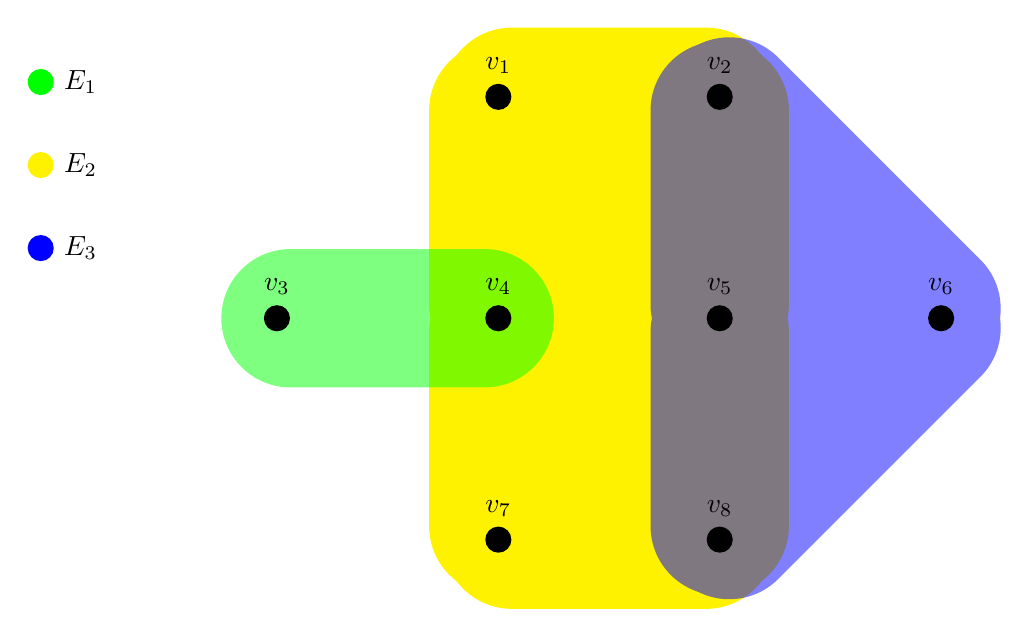
\begin{tikzpicture}
    \tikzstyle{vertex} = [fill,shape=circle,node distance=80pt]
\tikzstyle{edge} = [fill,opacity=.5,fill opacity=.5,line cap=round, line join=round, line width=50pt]
\tikzstyle{edge2} = [fill,opacity=.5,fill opacity=.5,line cap=round, line join=round, line width=30pt]
\tikzstyle{edge3} = [fill,opacity=1,fill opacity=1,line cap=round, line join=round, line width=50pt]

\tikzstyle{elabel} =  [fill,shape=circle,node distance=30pt]

\pgfdeclarelayer{background}
\pgfsetlayers{background,main}

\node[vertex,label=above:\(v_3\)] (v3) {};
\node[vertex,right of=v3,label=above:\(v_4\)] (v4) {};
\node[vertex,above of=v4,label=above:\(v_1\)] (v1) {};
\node[vertex,right of=v4,label=above:\(v_5\)] (v5) {};
\node[vertex,above of=v5,label=above:\(v_2\)] (v2) {};

\node[vertex,right of=v5,label=above:\(v_6\)] (v6) {};
\node[vertex,below of=v4,label=above:\(v_7\)] (v7) {};
\node[vertex,right of=v7,label=above:\(v_8\)] (v8) {};

\begin{pgfonlayer}{background}
\begin{scope}[transparency group,opacity=1]
\draw[edge3,color=yellow] (v1) -- (v2);
\draw[edge3,color=yellow] (v2) -- (v4);

\draw[edge3,color=yellow] (v1) -- (v4);
\draw[edge3,color=yellow] (v4) -- (v7);
\draw[edge3,color=yellow] (v2) -- (v5);
\draw[edge3,color=yellow] (v5) -- (v8);
\draw[edge3,color=yellow] (v5) -- (v7);

\draw[edge3,color=yellow] (v4) -- (v5);
\draw[edge3,color=yellow] (v7) -- (v8);
\end{scope}
\begin{scope}[transparency group,opacity=.5]
\draw[edge,opacity=1,color=green] (v3) -- (v4);
\fill[edge,opacity=1,color=green] (v3.center) -- (v4.center);
\end{scope}
\begin{scope}[transparency group,opacity=.5]
\draw[edge,opacity=1,color=blue] (v5) -- (v6);
\fill[edge,opacity=1,color=blue] (v5.center) -- (v6.center);
\draw[edge,opacity=1,color=blue] (v2) -- (v6);
\fill[edge,opacity=1,color=blue] (v2.center) -- (v6.center);
\draw[edge,opacity=1,color=blue] (v8) -- (v6);
\fill[edge,opacity=1,color=blue] (v8.center) -- (v6.center);
\draw[edge,opacity=1,color=blue] (v2) -- (v5)--(v8);
\fill[edge,opacity=1,color=blue] (v8.center) -- (v6.center);
\end{scope}


\end{pgfonlayer}

\node[elabel,color=green,label=right:\(E_1\)]  (e1) at (-3,3) {};
\node[elabel,below of=e1,color=yellow,label=right:\(E_2\)]  (e2) {};
\node[elabel,below of=e2,color=blue,label=right:\(E_3\)]  (e3) {};
\end{tikzpicture}
\end{center}

  Let $\hgrafeen_2$ be the following hypergraph:
  
  \begin{center}
   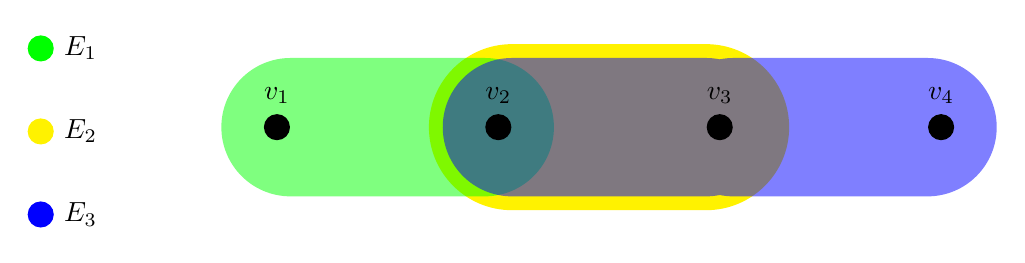
\begin{tikzpicture}
    \tikzstyle{vertex} = [fill,shape=circle,node distance=80pt]
\tikzstyle{edge} = [fill,opacity=.5,fill opacity=.5,line cap=round, line join=round, line width=50pt]
\tikzstyle{edge2} = [fill,opacity=.5,fill opacity=.5,line cap=round, line join=round, line width=30pt]
\tikzstyle{edge3} = [fill,opacity=1,fill opacity=1,line cap=round, line join=round, line width=60pt]

\tikzstyle{elabel} =  [fill,shape=circle,node distance=30pt]

\pgfdeclarelayer{background}
\pgfsetlayers{background,main}

\node[vertex,label=above:\(v_1\)] (v1) {};
\node[vertex,right of=v1,label=above:\(v_2\)] (v2) {};
\node[vertex,right of=v2,label=above:\(v_3\)] (v3) {};
\node[vertex,right of=v3,label=above:\(v_4\)] (v4) {};


\begin{pgfonlayer}{background}
\begin{scope}[transparency group,opacity=1]
\draw[edge3,color=yellow] (v2) -- (v3);

\end{scope}
\begin{scope}[transparency group,opacity=.5]
\draw[edge,opacity=1,color=green] (v1) -- (v2);
\fill[edge,opacity=1,color=green] (v1.center) -- (v2.center);
\end{scope}
\begin{scope}[transparency group,opacity=.5]
\draw[edge,opacity=1,color=blue] (v2)--(v3) -- (v4);
\fill[edge,opacity=1,color=blue] (v3.center) -- (v4.center);
\end{scope}


\end{pgfonlayer}

\node[elabel,color=green,label=right:\(E_1\)]  (e1) at (-3,1) {};
\node[elabel,below of=e1,color=yellow,label=right:\(E_2\)]  (e2) {};
\node[elabel,below of=e2,color=blue,label=right:\(E_3\)]  (e3) {};
\end{tikzpicture}
\end{center}

 And let $\hgrafeen_3$ be the following hypergraph ($\hgrafeen_3$ is in fact also an undirected graph):
  \begin{center}
   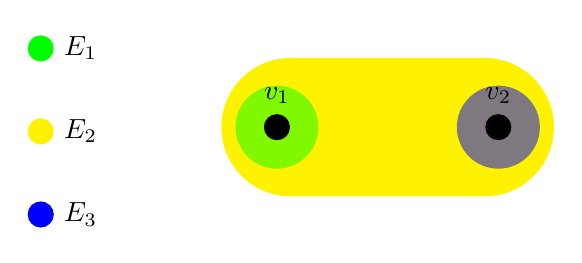
\begin{tikzpicture}
    \tikzstyle{vertex} = [fill,shape=circle,node distance=80pt]
\tikzstyle{edge} = [fill,opacity=.5,fill opacity=.5,line cap=round, line join=round, line width=50pt]
\tikzstyle{edge2} = [fill,opacity=.5,fill opacity=.5,line cap=round, line join=round, line width=30pt]
\tikzstyle{edge3} = [fill,opacity=1,fill opacity=1,line cap=round, line join=round, line width=50pt]

\tikzstyle{elabel} =  [fill,shape=circle,node distance=30pt]

\pgfdeclarelayer{background}
\pgfsetlayers{background,main}

\node[vertex,label=above:\(v_1\)] (v1) {};
\node[vertex,right of=v1,label=above:\(v_2\)] (v2) {};



\begin{pgfonlayer}{background}
\begin{scope}[transparency group,opacity=1]
\draw[edge3,color=yellow] (v1) -- (v2);

\end{scope}
\begin{scope}[transparency group,opacity=.5]
\draw[edge2,opacity=1,color=green] (v1) -- (v1);
\end{scope}
\begin{scope}[transparency group,opacity=.5]
\draw[edge2,opacity=1,color=blue] (v2) -- (v2);
\end{scope}


\end{pgfonlayer}

\node[elabel,color=green,label=right:\(E_1\)]  (e1) at (-3,1) {};
\node[elabel,below of=e1,color=yellow,label=right:\(E_2\)]  (e2) {};
\node[elabel,below of=e2,color=blue,label=right:\(E_3\)]  (e3) {};
\end{tikzpicture}
\end{center}
All off $\hgrafeen_1, \hgrafeen_2$ and $\hgrafeen_3$ lead to the same line-graph 
$\graf$:
\begin{center}
\begin{tikzpicture}[<->,>=stealth',shorten >=1pt,auto,node distance=3cm,
                    thick]
                    \tikzstyle{every node}=[draw,circle,fill=black,minimum size=4pt,
                            inner sep=0pt]


  \node[main node] (1) [label=above:$E_1$] {};
  \node[main node] (2) [label=above:$E_2$][right of=1] {};
  \node[main node] (3) [label=above:$E_3$][right of=2] {};;

  \path[every node/.style={font=\sffamily\small}]
   
    (1) edge node [left] {} (2)
      (2) edge node [left] {} (3)
    
\end{tikzpicture}
\end{center}
\end{example}
\subsubsection{Algorithm for similarity}
We want to apply Algorithm \ref{algsimilarity} to produce a similarity matrix
between two hypergraphs. This will produces an edge similarity matrix, because the vertices are not represented in the line-graph representation. 


To use Algorithm \ref{algsimilarity} from section 2.2, we first take a hypergraph as input and calculate the adjacency matrix of 
the corresponding line-graph. The Matlab implementation of this step can be found in Appendix \ref{appendixa} in Listing \ref{linealgmatlab}. By applying this algorithm to two hypergraphs, we 
can use Algorithm \ref{algsimilarity}. 

\subsubsection{Examples}
We now give some examples of the similarity of two hypergraphs by using 
line-graphs:
\begin{example}\label{ex1line}
  Let $\hgrafeen_1$ be the following hypergraph:
     \begin{center}
   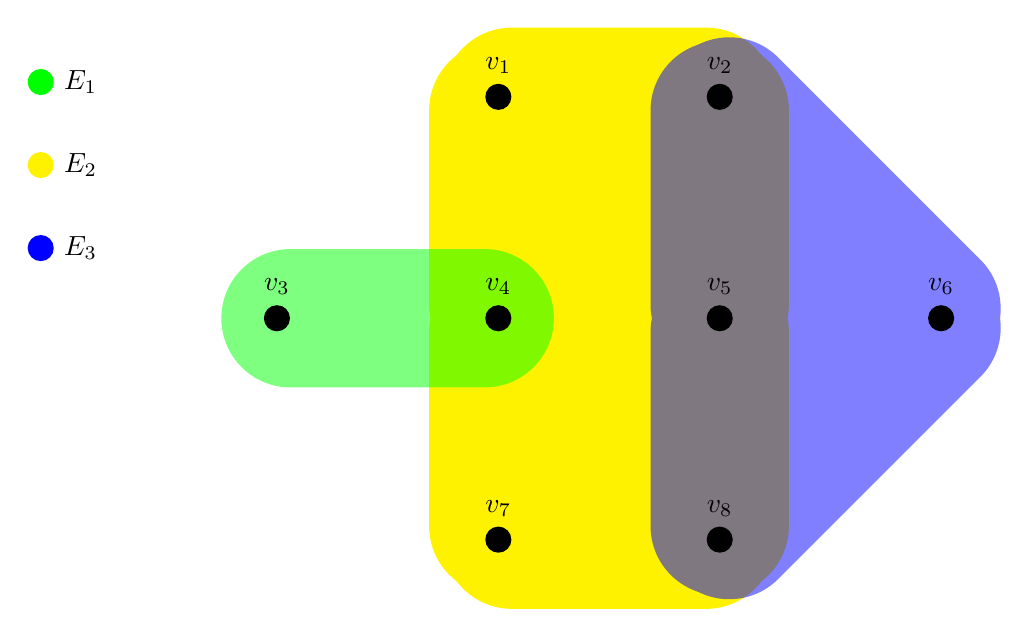
\begin{tikzpicture}
    \tikzstyle{vertex} = [fill,shape=circle,node distance=80pt]
\tikzstyle{edge} = [fill,opacity=.5,fill opacity=.5,line cap=round, line join=round, line width=50pt]
\tikzstyle{edge2} = [fill,opacity=.5,fill opacity=.5,line cap=round, line join=round, line width=30pt]
\tikzstyle{edge3} = [fill,opacity=1,fill opacity=1,line cap=round, line join=round, line width=50pt]

\tikzstyle{elabel} =  [fill,shape=circle,node distance=30pt]

\pgfdeclarelayer{background}
\pgfsetlayers{background,main}

\node[vertex,label=above:\(v_3\)] (v3) {};
\node[vertex,right of=v3,label=above:\(v_4\)] (v4) {};
\node[vertex,above of=v4,label=above:\(v_1\)] (v1) {};
\node[vertex,right of=v4,label=above:\(v_5\)] (v5) {};
\node[vertex,above of=v5,label=above:\(v_2\)] (v2) {};

\node[vertex,right of=v5,label=above:\(v_6\)] (v6) {};
\node[vertex,below of=v4,label=above:\(v_7\)] (v7) {};
\node[vertex,right of=v7,label=above:\(v_8\)] (v8) {};

\begin{pgfonlayer}{background}
\begin{scope}[transparency group,opacity=1]
\draw[edge3,color=yellow] (v1) -- (v2);
\draw[edge3,color=yellow] (v2) -- (v4);

\draw[edge3,color=yellow] (v1) -- (v4);
\draw[edge3,color=yellow] (v4) -- (v7);
\draw[edge3,color=yellow] (v2) -- (v5);
\draw[edge3,color=yellow] (v5) -- (v8);
\draw[edge3,color=yellow] (v5) -- (v7);

\draw[edge3,color=yellow] (v4) -- (v5);
\draw[edge3,color=yellow] (v7) -- (v8);
\end{scope}
\begin{scope}[transparency group,opacity=.5]
\draw[edge,opacity=1,color=green] (v3) -- (v4);
\fill[edge,opacity=1,color=green] (v3.center) -- (v4.center);
\end{scope}
\begin{scope}[transparency group,opacity=.5]
\draw[edge,opacity=1,color=blue] (v5) -- (v6);
\fill[edge,opacity=1,color=blue] (v5.center) -- (v6.center);
\draw[edge,opacity=1,color=blue] (v2) -- (v6);
\fill[edge,opacity=1,color=blue] (v2.center) -- (v6.center);
\draw[edge,opacity=1,color=blue] (v8) -- (v6);
\fill[edge,opacity=1,color=blue] (v8.center) -- (v6.center);
\draw[edge,opacity=1,color=blue] (v2) -- (v5)--(v8);
\fill[edge,opacity=1,color=blue] (v8.center) -- (v6.center);
\end{scope}


\end{pgfonlayer}

\node[elabel,color=green,label=right:\(E_1\)]  (e1) at (-3,3) {};
\node[elabel,below of=e1,color=yellow,label=right:\(E_2\)]  (e2) {};
\node[elabel,below of=e2,color=blue,label=right:\(E_3\)]  (e3) {};
\end{tikzpicture}
\end{center}

  Let $\hgrafeen_2$ be the following hypergraph:
   \begin{center}
   \begin{tikzpicture}
    \tikzstyle{vertex} = [fill,shape=circle,node distance=60pt]
\tikzstyle{edge} = [fill,opacity=.5,fill opacity=.5,line cap=round, line join=round, line width=50pt]
\tikzstyle{edge2} = [fill,opacity=.5,fill opacity=.5,line cap=round, line join=round, line width=30pt]
\tikzstyle{edge3} = [fill,opacity=1,fill opacity=1,line cap=round, line join=round, line width=50pt]

\tikzstyle{elabel} =  [fill,shape=circle,node distance=30pt]

\pgfdeclarelayer{background}
\pgfsetlayers{background,main}

\node[vertex,label=above:\(v_4\)] (v4) {};
\node[vertex,right of=v3,label=above:\(v_5\)] (v5) {};
\node[vertex,right of=v5,label=above:\(v_6\)] (v6) {};

\node[vertex,right of=v6,label=above:\(v_7\)] (v7) {};
\node[vertex,right of=v7,label=above:\(v_8\)] (v8) {};
\node[vertex,right of=v8,label=above:\(v_9\)] (v9) {};
\node[vertex,above of=v6,label=above:\(v_1\)] (v1) {};

\node[vertex,above of=v8,label=above:\(v_3\)] (v3) {};
\node[vertex,above of=v7,label=above:\(v_2\)] (v2) {};


\node[vertex,below of=v6,label=above:\(v_{10}\)] (v10) {};
\node[vertex,right of=v10,label=above:\(v_{11}\)] (v11) {};
\node[vertex,right of=v11,label=above:\(v_{12}\)] (v12) {};


\begin{pgfonlayer}{background}
\begin{scope}[transparency group,opacity=1]
\draw[edge3,color=yellow] (v1) -- (v2);
\draw[edge3,color=yellow] (v2) -- (v7);
\draw[edge3,color=yellow] (v11) -- (v7);
\draw[edge3,color=yellow] (v1) -- (v6);
\draw[edge3,color=yellow] (v1) -- (v7);
\draw[edge3,color=yellow] (v6) -- (v7);
\draw[edge3,color=yellow] (v6) -- (v11);
\draw[edge3,color=yellow] (v6) -- (v10);

\draw[edge3,color=yellow] (v10) -- (v11);

\end{scope}
\begin{scope}[transparency group,opacity=.5]
\draw[edge,opacity=1,color=green] (v4) -- (v5);
\fill[edge,opacity=1,color=green] (v4.center) -- (v5.center);
\end{scope}
\begin{scope}[transparency group,opacity=.5]
\draw[edge,opacity=1,color=blue] (v3) -- (v8);
\fill[edge,opacity=1,color=blue] (v3.center) -- (v8.center);
\draw[edge,opacity=1,color=blue] (v3) -- (v9);
\fill[edge,opacity=1,color=blue] (v3.center) -- (v9.center);
\draw[edge,opacity=1,color=blue] (v9) -- (v8);
\draw[edge,opacity=1,color=blue] (v9) -- (v12);
\fill[edge,opacity=1,color=blue] (v8.center) -- (v6.center);
\draw[edge,opacity=1,color=blue] (v3) -- (v8)--(v12);
\fill[edge,opacity=1,color=blue] (v8.center) -- (v6.center);
\end{scope}
\draw[edge,color=purple] (v5) -- (v6)--(v7)--(v8);


\end{pgfonlayer}

\node[elabel,color=green,label=right:\(E'_1\)]  (e1) at (-3,3) {};
\node[elabel,below of=e1,color=yellow,label=right:\(E'_2\)]  (e2) {};
\node[elabel,below of=e2,color=blue,label=right:\(E'_3\)]  (e3) {};
\node[elabel,below of=e3,color=purple,label=right:\(E'_4\)]  (e4) {};

\end{tikzpicture}
\end{center}

By applying the algorithm we get the adjacency matrices $A_1$ for 
 $\hgrafeen_1$ and $A_2$ for $\hgrafeen_2$:
 $$A_1 = \begin{pmatrix}
  0 & 1 & 0\\
 1 & 0 & 1\\
  0 & 1 & 0
 \end{pmatrix} \quad \text{and} \quad
 A_2 = \begin{pmatrix}
     0 & 0 & 0 & 1\\
     0 & 0 & 0 & 1\\
     0 & 0 & 0 & 1\\
     1 & 1 & 1 & 0
 \end{pmatrix}
 
 
 Now we use Algorithm \ref{algsimilarity} with $A_1$ and $A_2$ and get the following similarity matrix:
  $$ S = \begin{pmatrix}
      0.2887 &    0.2887  & 0.2887\\
    0.2887  & 0.2887   & 0.2887\\
    0.2887   & 0.2887  & 0.2887\\
    0.2887  &  0.2887  & 0.2887
    \end{pmatrix}$$
    
   \end{example}

\begin{example}\label{ex2line}
  $\hgrafeen_1$ is the same as in the previous example, but now, $\hgrafeen_2$ 
  is the following hypergraph:
   \begin{center}
   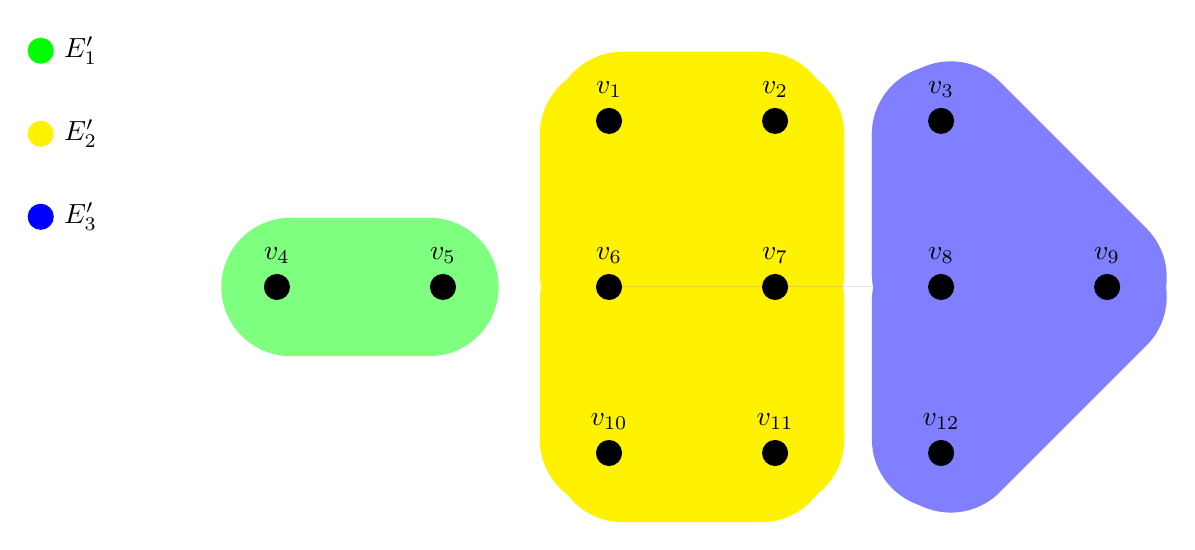
\begin{tikzpicture}
    \tikzstyle{vertex} = [fill,shape=circle,node distance=60pt]
\tikzstyle{edge} = [fill,opacity=.5,fill opacity=.5,line cap=round, line join=round, line width=50pt]
\tikzstyle{edge2} = [fill,opacity=.5,fill opacity=.5,line cap=round, line join=round, line width=30pt]
\tikzstyle{edge3} = [fill,opacity=1,fill opacity=1,line cap=round, line join=round, line width=50pt]

\tikzstyle{elabel} =  [fill,shape=circle,node distance=30pt]

\pgfdeclarelayer{background}
\pgfsetlayers{background,main}

\node[vertex,label=above:\(v_4\)] (v4) {};
\node[vertex,right of=v4,label=above:\(v_5\)] (v5) {};
\node[vertex,right of=v5,label=above:\(v_6\)] (v6) {};

\node[vertex,right of=v6,label=above:\(v_7\)] (v7) {};
\node[vertex,right of=v7,label=above:\(v_8\)] (v8) {};
\node[vertex,right of=v8,label=above:\(v_9\)] (v9) {};
\node[vertex,above of=v6,label=above:\(v_1\)] (v1) {};

\node[vertex,above of=v8,label=above:\(v_3\)] (v3) {};
\node[vertex,above of=v7,label=above:\(v_2\)] (v2) {};


\node[vertex,below of=v6,label=above:\(v_{10}\)] (v10) {};
\node[vertex,right of=v10,label=above:\(v_{11}\)] (v11) {};
\node[vertex,right of=v11,label=above:\(v_{12}\)] (v12) {};


\begin{pgfonlayer}{background}
\begin{scope}[transparency group,opacity=1]
\draw[edge3,color=yellow] (v1) -- (v2);
\draw[edge3,color=yellow] (v2) -- (v7);
\draw[edge3,color=yellow] (v11) -- (v7);
\draw[edge3,color=yellow] (v1) -- (v6);
\draw[edge3,color=yellow] (v1) -- (v7);
\draw[edge3,color=yellow] (v6) -- (v7);
\draw[edge3,color=yellow] (v6) -- (v11);
\draw[edge3,color=yellow] (v6) -- (v10);

\draw[edge3,color=yellow] (v10) -- (v11);

\end{scope}
\begin{scope}[transparency group,opacity=.5]
\draw[edge,opacity=1,color=green] (v4) -- (v5);
\fill[edge,opacity=1,color=green] (v4.center) -- (v5.center);
\end{scope}
\begin{scope}[transparency group,opacity=.5]
\draw[edge,opacity=1,color=blue] (v3) -- (v8);
\fill[edge,opacity=1,color=blue] (v3.center) -- (v8.center);
\draw[edge,opacity=1,color=blue] (v3) -- (v9);
\fill[edge,opacity=1,color=blue] (v3.center) -- (v9.center);
\draw[edge,opacity=1,color=blue] (v9) -- (v8);
\draw[edge,opacity=1,color=blue] (v9) -- (v12);
\fill[edge,opacity=1,color=blue] (v8.center) -- (v6.center);
\draw[edge,opacity=1,color=blue] (v3) -- (v8)--(v12);
\fill[edge,opacity=1,color=blue] (v8.center) -- (v6.center);
\end{scope}


\end{pgfonlayer}

\node[elabel,color=green,label=right:\(E'_1\)]  (e1) at (-3,3) {};
\node[elabel,below of=e1,color=yellow,label=right:\(E'_2\)]  (e2) {};
\node[elabel,below of=e2,color=blue,label=right:\(E'_3\)]  (e3) {};

\end{tikzpicture}
\end{center}
  The similarity score of these two hypergraphs by using their line-graph representation becomes:
  $$S = \begin{pmatrix}
  0 & 0 & 0\\
  0 & 0 & 0\\
  0 & 0 & 0
  \end{pmatrix}$$

\end{example}

\begin{example}\label{ex3line}
  $\hgrafeen_1$ is the same as in the previous example, but now, $\hgrafeen_2$ 
  is the following hypergraph:
   \begin{center}
   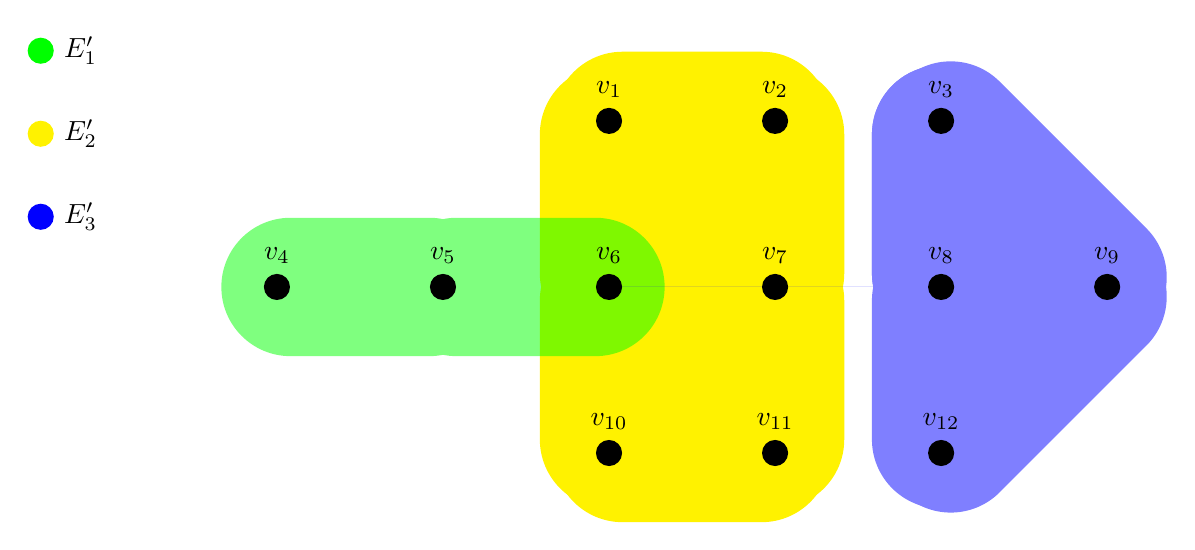
\begin{tikzpicture}
    \tikzstyle{vertex} = [fill,shape=circle,node distance=60pt]
\tikzstyle{edge} = [fill,opacity=.5,fill opacity=.5,line cap=round, line join=round, line width=50pt]
\tikzstyle{edge2} = [fill,opacity=.5,fill opacity=.5,line cap=round, line join=round, line width=30pt]
\tikzstyle{edge3} = [fill,opacity=1,fill opacity=1,line cap=round, line join=round, line width=50pt]

\tikzstyle{elabel} =  [fill,shape=circle,node distance=30pt]

\pgfdeclarelayer{background}
\pgfsetlayers{background,main}

\node[vertex,label=above:\(v_4\)] (v4) {};
\node[vertex,right of=v4,label=above:\(v_5\)] (v5) {};
\node[vertex,right of=v5,label=above:\(v_6\)] (v6) {};

\node[vertex,right of=v6,label=above:\(v_7\)] (v7) {};
\node[vertex,right of=v7,label=above:\(v_8\)] (v8) {};
\node[vertex,right of=v8,label=above:\(v_9\)] (v9) {};
\node[vertex,above of=v6,label=above:\(v_1\)] (v1) {};

\node[vertex,above of=v8,label=above:\(v_3\)] (v3) {};
\node[vertex,above of=v7,label=above:\(v_2\)] (v2) {};


\node[vertex,below of=v6,label=above:\(v_{10}\)] (v10) {};
\node[vertex,right of=v10,label=above:\(v_{11}\)] (v11) {};
\node[vertex,right of=v11,label=above:\(v_{12}\)] (v12) {};


\begin{pgfonlayer}{background}
\begin{scope}[transparency group,opacity=1]
\draw[edge3,color=yellow] (v1) -- (v2);
\draw[edge3,color=yellow] (v2) -- (v7);
\draw[edge3,color=yellow] (v11) -- (v7);
\draw[edge3,color=yellow] (v1) -- (v6);
\draw[edge3,color=yellow] (v1) -- (v7);
\draw[edge3,color=yellow] (v6) -- (v7);
\draw[edge3,color=yellow] (v6) -- (v11);
\draw[edge3,color=yellow] (v6) -- (v10);

\draw[edge3,color=yellow] (v10) -- (v11);

\end{scope}
\begin{scope}[transparency group,opacity=.5]
\draw[edge,opacity=1,color=green] (v4) -- (v5)--(v6);
\fill[edge,opacity=1,color=green] (v4.center) -- (v5.center) -- (v6.center);
\end{scope}
\begin{scope}[transparency group,opacity=.5]
\draw[edge,opacity=1,color=blue] (v3) -- (v8);
\fill[edge,opacity=1,color=blue] (v3.center) -- (v8.center);
\draw[edge,opacity=1,color=blue] (v3) -- (v9);
\fill[edge,opacity=1,color=blue] (v3.center) -- (v9.center);
\draw[edge,opacity=1,color=blue] (v9) -- (v8);
\draw[edge,opacity=1,color=blue] (v9) -- (v12);
\fill[edge,opacity=1,color=blue] (v8.center) -- (v6.center);
\draw[edge,opacity=1,color=blue] (v3) -- (v8)--(v12);
\fill[edge,opacity=1,color=blue] (v8.center) -- (v6.center);
\end{scope}


\end{pgfonlayer}

\node[elabel,color=green,label=right:\(E'_1\)]  (e1) at (-3,3) {};
\node[elabel,below of=e1,color=yellow,label=right:\(E'_2\)]  (e2) {};
\node[elabel,below of=e2,color=blue,label=right:\(E'_3\)]  (e3) {};

\end{tikzpicture}
\end{center}
  The similarity score of these two hypergraphs by using their line-graph representation becomes:
  $$S = \begin{pmatrix}
    0.4082 &    0.4082  &  0.4082\\
    0.4082 &    0.4082  &   0.4082\\
         0      &   0   &      0
  \end{pmatrix}$$

  \end{example}
  
  \begin{example}\label{ex4line}
  $\hgrafeen_1$ is the same as in the previous example, but now, $\hgrafeen_2$ 
  is the following hypergraph:
     \begin{center}
   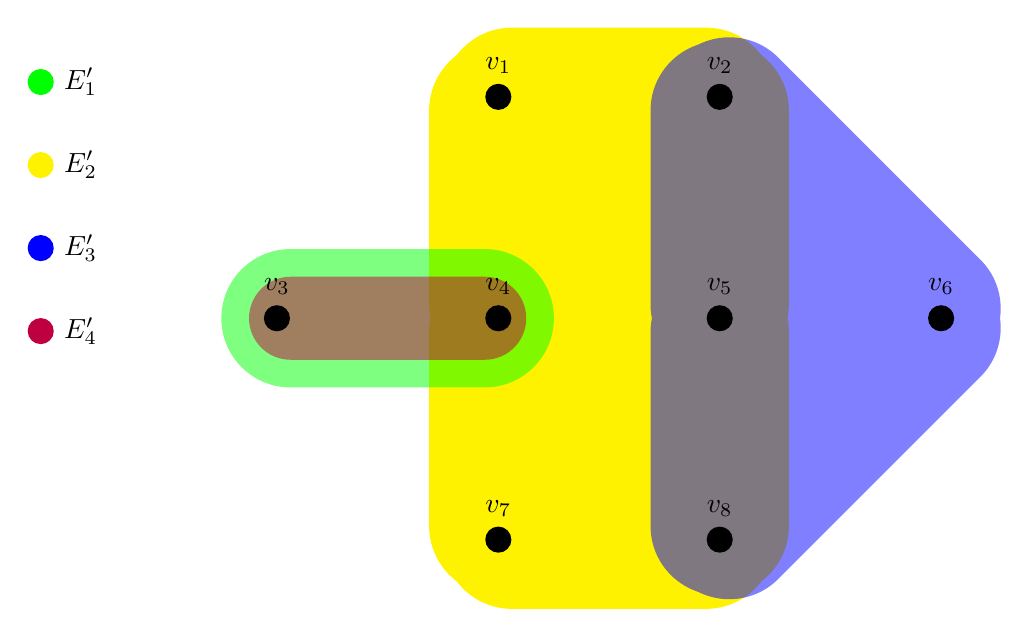
\begin{tikzpicture}
    \tikzstyle{vertex} = [fill,shape=circle,node distance=80pt]
\tikzstyle{edge} = [fill,opacity=.5,fill opacity=.5,line cap=round, line join=round, line width=50pt]
\tikzstyle{edge2} = [fill,opacity=.5,fill opacity=.5,line cap=round, line join=round, line width=30pt]
\tikzstyle{edge3} = [fill,opacity=1,fill opacity=1,line cap=round, line join=round, line width=50pt]

\tikzstyle{elabel} =  [fill,shape=circle,node distance=30pt]

\pgfdeclarelayer{background}
\pgfsetlayers{background,main}

\node[vertex,label=above:\(v_3\)] (v3) {};
\node[vertex,right of=v3,label=above:\(v_4\)] (v4) {};
\node[vertex,above of=v4,label=above:\(v_1\)] (v1) {};
\node[vertex,right of=v4,label=above:\(v_5\)] (v5) {};
\node[vertex,above of=v5,label=above:\(v_2\)] (v2) {};

\node[vertex,right of=v5,label=above:\(v_6\)] (v6) {};
\node[vertex,below of=v4,label=above:\(v_7\)] (v7) {};
\node[vertex,right of=v7,label=above:\(v_8\)] (v8) {};

\begin{pgfonlayer}{background}
\begin{scope}[transparency group,opacity=1]
\draw[edge3,color=yellow] (v1) -- (v2);
\draw[edge3,color=yellow] (v2) -- (v4);

\draw[edge3,color=yellow] (v1) -- (v4);
\draw[edge3,color=yellow] (v4) -- (v7);
\draw[edge3,color=yellow] (v2) -- (v5);
\draw[edge3,color=yellow] (v5) -- (v8);
\draw[edge3,color=yellow] (v5) -- (v7);

\draw[edge3,color=yellow] (v4) -- (v5);
\draw[edge3,color=yellow] (v7) -- (v8);
\end{scope}
\begin{scope}[transparency group,opacity=.5]
\draw[edge,opacity=1,color=green] (v3) -- (v4);
\fill[edge,opacity=1,color=green] (v3.center) -- (v4.center);
\end{scope}
\begin{scope}[transparency group,opacity=.5]
\draw[edge2,opacity=1,color=purple] (v3) -- (v4);
\fill[edge2,opacity=1,color=purple] (v3.center) -- (v4.center);
\end{scope}
\begin{scope}[transparency group,opacity=.5]
\draw[edge,opacity=1,color=blue] (v5) -- (v6);
\fill[edge,opacity=1,color=blue] (v5.center) -- (v6.center);
\draw[edge,opacity=1,color=blue] (v2) -- (v6);
\fill[edge,opacity=1,color=blue] (v2.center) -- (v6.center);
\draw[edge,opacity=1,color=blue] (v8) -- (v6);
\fill[edge,opacity=1,color=blue] (v8.center) -- (v6.center);
\draw[edge,opacity=1,color=blue] (v2) -- (v5)--(v8);
\fill[edge,opacity=1,color=blue] (v8.center) -- (v6.center);
\end{scope}


\end{pgfonlayer}

\node[elabel,color=green,label=right:\(E'_1\)]  (e1) at (-3,3) {};
\node[elabel,below of=e1,color=yellow,label=right:\(E'_2\)]  (e2) {};
\node[elabel,below of=e2,color=blue,label=right:\(E'_3\)]  (e3) {};
\node[elabel,below of=e3,color=purple,label=right:\(E'_4\)]  (e4) {};

\end{tikzpicture}
\end{center}
  The similarity score of these two hypergraphs by using their line-graph representation becomes:
  $$S = \begin{pmatrix}
    0.4082 &    0.4082  & 0 & 0.4082 \\
    0.4082 &    0.4082  &  0&  0.4082 \\
         0      &   0   &      0 & 0
  \end{pmatrix}$$

  \end{example}
  
  \subsubsection{Interpretation}
  We now discuss the conditions from the introduction:
  \begin{itemize}
    \item[(C1)] Not fulfilled: first, the method will only return an edge 
    similarity matrix and second, the line-graph of an undirected graph is not 
    necessary the undirected graph itself:
    \begin{center}
\begin{tikzpicture}[<->,>=stealth',shorten >=1pt,auto,node distance=3cm,
                    thick]
                    \tikzstyle{every node}=[draw,circle,fill=black,minimum size=4pt,
                            inner sep=0pt]


  \node[main node] (1) [label=above:$v_1$] {};
  \node[main node] (2) [label=above:$v_2$][right of=1] {};
  \node[main node] (3) [label=above:$v_3$][right of=2] {};;

  \path[every node/.style={font=\sffamily\small}]
   
    (1) edge node [above] {$e_1$} (2)
      (2) edge node [above] {$e_2$} (3)
    
\end{tikzpicture}
\end{center}
Has as line-graph:

        \begin{center}
\begin{tikzpicture}[<->,>=stealth',shorten >=1pt,auto,node distance=3cm,
                    thick]
                    \tikzstyle{every node}=[draw,circle,fill=black,minimum size=4pt,
                            inner sep=0pt]


  \node[main node] (1) [label=above:$e_1$] {};
  \node[main node] (2) [label=above:$e_2$][right of=1] {};


  \path[every node/.style={font=\sffamily\small}]
   
    (1) edge node [above] {} (2)
    
\end{tikzpicture}
\end{center}
which will clearly not result in the same edge similarity scores as no 
information about the vertex adjacency is saved.
    
    
 
 
   \item[(C2)] Not fulfilled: the vertices of the hypergraph don't play a role 
   in the line-graph. No information about them is saved in the line-graph 
   representation.
  \item[(C3)] Fulfilled: Adding an edge to one of the two hypergraphs will 
  result in an extra vertex in the line-graph. Adding this vertex will take the 
  edge into account when calculating the similarity scores and therefore we 
  conclude on a heuristic base that this condition is fulfilled.
  \item[(C4)] Not fulfilled: in Examples \ref{ex1line}, \ref{ex2line}, \ref{ex3line}  
  and \ref{ex4line}
  all positive similarity scores are the same, regardless of the adjacency 
  structure of the hypergraph.
  \item[(C5)] Not fulfilled: there is no information about the vertices saved in 
  the line-graph representation of a hypergraph.
  \item[(C6)] Fulfilled: from Example \ref{ex4line} we see that the $E'_1$ and 
 $E'_4$ are structural equivalent and have indeed the same similarity scores. We will 
 prove this.
 
 \begin{theorem}
   The line-graph representation of a hypergraph preserves structural equivalent 
   edges.
 \end{theorem}
 \begin{proof}
   Two edges are structural equivalent in a hypergraph if they contain exactly the same 
   vertices. They form an equivalence class on $E$ where $E_i \sim E_j$ if they 
   are structural equivalent. Let $\overline{E_i}$ be the class of structural equivalent 
   edges with $E_i$, we assume that this class contains at least 2 edges. Now from definition \ref{linegraphdef} we see that
   $E_i \leftrightarrow E_j$ if and only if $E_i \cap E_j \not = \emptyset$ and $i \not = j$ 
   in the linegraph representation, thus all the edges in $\overline{E_i}$ will 
   have exactly the same adjacency structure, making them structural equivalent as vertices in the 
   line-graph representation too.
 \end{proof}
 Because the line-graph representation preserves structural equivalent edges and we use the method of Blondel for which we already proved
 in (E6) that this condition holds, the result follows.
     \item[(C7)] Not fulfilled: no information on the number of vertices an edge 
contains is preserverd by the line-graph representation.
  \item[(C8)] Fulfilled: but it is also the only thing this representation tells us 
  when used for the calculation of similarity: two edges of the two line-graphs
  have a positive similarity score when these edges are connected to other edges, meaning that for any $E_p, E_q$ there is a sequence 
  $$E_p = E_{k_0}, E_{k_1}, \ldots, E_{k_{l-1}}, E_q = E_{k_l}$$
  such that $E_{k_{i-1}} \cap E_{k_i} \not = \emptyset$. 
  
  
 This follows immediately from  Property \ref{linegrafconnected}. The connectivity 
  of edges is indeed represented in the line-graph representation by definition. 
  

  \end{itemize}  
  \subsubsection{Conclusion}
  The line-graph fails to satisfy lots of the conditions and is therefore 
  not a good representation to calculate similarity between two hypergraphs. 
  Similarity between hypergraphs through line-graphs only allows us to discover 
  groups of connected edges in both hypergraphs. The fact that the line-graph 
  representation is a bit disappointing, was also predictable as a lot of 
  hypergraphs share the same line-graph representation. 


\subsection{$2$-section of a hypergraph}\index{$2$-section}\index{hypergraph representation!$2$-section}

\subsubsection{General definitions and properties}
We now look at another graph representation of a hypergraph. In contrast to the 
line-graph representation, the $2$-section saves information about the vertices 
which will introduce a more sophisticated way to say something about 
similarity between two hypergraphs by using their $2$-section.

\begin{definition}
  The \textbf{$2$-section} of a hypergraph $\hgrafeen = (V,E)$ is the (undirected) graph denoted by $\[\hgrafeen\]_2 = (V,\leftrightarrow)$ 
  with:
  \begin{itemize}
    \item The same vertex set as the hypergraph,
    \item $v_i \leftrightarrow v_j$ if and only if $v_i, v_j \in E_k$ for some $E_k \in E$ and $i \not = j$.
  \end{itemize}
  \end{definition}
  
\begin{example}\label{uniciteitsvoorbeeld}
The 2-section of the following hypergraph $\hgrafeen$ is drawn on top:
    \begin{center}
   \begin{tikzpicture}
    \tikzstyle{vertex} = [fill,shape=circle,node distance=80pt]
\tikzstyle{edge} = [fill,opacity=.5,fill opacity=.5,line cap=round, line join=round, line width=50pt]
\tikzstyle{edge2} = [fill,opacity=.5,fill opacity=.5,line cap=round, line join=round, line width=30pt]
\tikzstyle{edge3} = [fill,opacity=1,fill opacity=1,line cap=round, line join=round, line width=50pt]
\tikzstyle{gedge} = [<->,>=stealth',shorten >=1pt, auto,node distance=3cm,
                    thick]
                    \tikzstyle{gedge30} = [<->,>=stealth',shorten >=1pt,bend right=30, auto,node distance=3cm,
                    thick]
\tikzstyle{elabel} =  [fill,shape=circle,node distance=30pt]

\pgfdeclarelayer{background}
\pgfsetlayers{background,main}

\node[vertex,label=above:\(v_3\)] (v3) {};
\node[vertex,right of=v3,label=above left:\(v_4\)] (v4) {};
\node[vertex,above of=v4,label=above:\(v_1\)] (v1) {};
\node[vertex,right of=v4,label=above right:\(v_5\)] (v5) {};
\node[vertex,above of=v5,label=above:\(v_2\)] (v2) {};

\node[vertex,right of=v5,label=above:\(v_6\)] (v6) {};
\node[vertex,below of=v4,label=below:\(v_7\)] (v7) {};
\node[vertex,right of=v7,label=below:\(v_8\)] (v8) {};



\begin{pgfonlayer}{background}
\begin{scope}[transparency group,opacity=1]
\draw[edge3,color=yellow] (v1) -- (v2);
\draw[edge3,color=yellow] (v2) -- (v4);

\draw[edge3,color=yellow] (v1) -- (v4);
\draw[edge3,color=yellow] (v4) -- (v7);
\draw[edge3,color=yellow] (v2) -- (v5);
\draw[edge3,color=yellow] (v5) -- (v8);
\draw[edge3,color=yellow] (v5) -- (v7);

\draw[edge3,color=yellow] (v4) -- (v5);
\draw[edge3,color=yellow] (v7) -- (v8);
\end{scope}
\begin{scope}[transparency group,opacity=.5]
\draw[edge,opacity=1,color=green] (v3) -- (v4);
\fill[edge,opacity=1,color=green] (v3.center) -- (v4.center);
\end{scope}
\begin{scope}[transparency group,opacity=.5]
\draw[edge,opacity=1,color=blue] (v5) -- (v6);
\fill[edge,opacity=1,color=blue] (v5.center) -- (v6.center);
\draw[edge,opacity=1,color=blue] (v2) -- (v6);
\fill[edge,opacity=1,color=blue] (v2.center) -- (v6.center);
\draw[edge,opacity=1,color=blue] (v8) -- (v6);
\fill[edge,opacity=1,color=blue] (v8.center) -- (v6.center);
\draw[edge,opacity=1,color=blue] (v2) -- (v5)--(v8);
\fill[edge,opacity=1,color=blue] (v8.center) -- (v6.center);
\end{scope}
\begin{scope}[transparency group,opacity=1]
  \draw[gedge,opacity=1,color=black] (v3) -- (v4);
  \draw[gedge,opacity=1,color=black] (v1) -- (v4);
  \draw[gedge,opacity=1,color=black] (v2) -- (v4);
   \draw[gedge,opacity=1,color=black] (v5) -- (v4);
  \draw[gedge,opacity=1,color=black] (v8) -- (v4);
  \draw[gedge,opacity=1,color=black] (v7) -- (v4);
   \draw[gedge,opacity=1,color=black] (v1) -- (v2);
  \draw[gedge,opacity=1,color=black] (v1) -- (v5);
  \draw[gedge,opacity=1,color=black] (v1) -- (v8);
   \draw[gedge30, bent left=100, opacity=1,color=black] (v1) -- (v7);
  \draw[gedge,opacity=1,color=black] (v2) -- (v5);
  \draw[gedge,opacity=1,color=black] (v2) -- (v8);
   \draw[gedge,opacity=1,color=black] (v2) -- (v7);
  \draw[gedge,opacity=1,color=black] (v2) -- (v6);
  \draw[gedge,opacity=1,color=black] (v5) -- (v7);
    \draw[gedge,opacity=1,color=black] (v5) -- (v8);
    \draw[gedge,opacity=1,color=black] (v5) -- (v6);
      \draw[gedge,opacity=1,color=black] (v8) -- (v6);
      \end{scope}
      \begin{scope}[transparency group,opacity=1]

      \draw[gedge30, opacity=1, bend left] (v1) -- (v7);
\end{scope}

\end{pgfonlayer}

\node[elabel,color=green,label=right:\(E_1\)]  (e1) at (-3,3) {};
\node[elabel,below of=e1,color=yellow,label=right:\(E_2\)]  (e2) {};
\node[elabel,below of=e2,color=blue,label=right:\(E_3\)]  (e3) {};
\end{tikzpicture}
\end{center}
\end{example}

Also the 2-section of a hypergraph is not a faithful graph characteristic of a hypergraph, as the following example 
shows:

\begin{example}\label{2sectievoorbeeld}
The 2-section of the following hypergraph $\hgrafeen'$ is drawn on top and is the same as the previous example:

      \begin{center}
   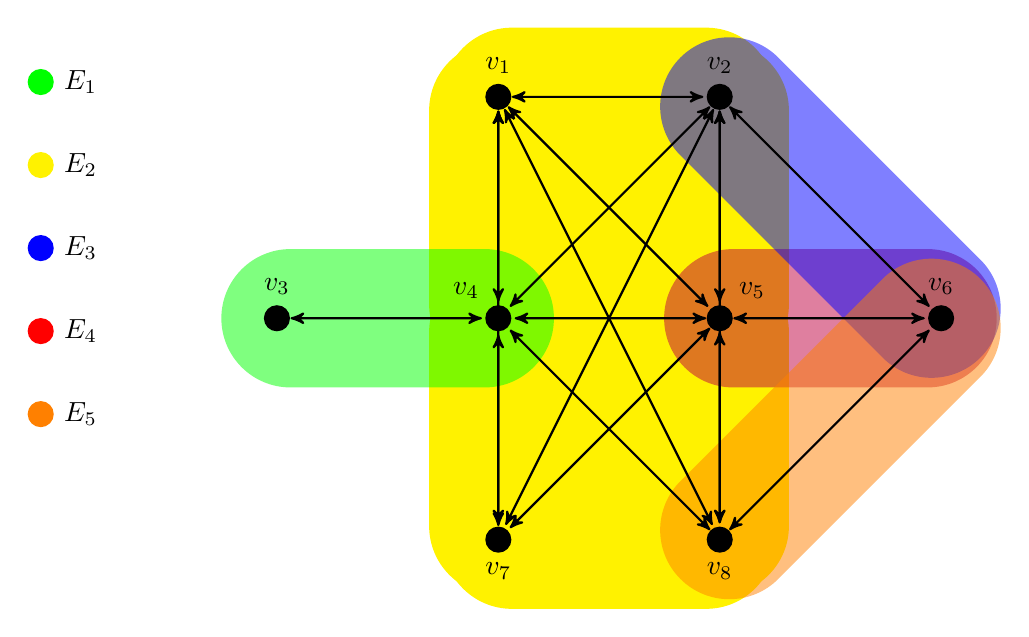
\begin{tikzpicture}
    \tikzstyle{vertex} = [fill,shape=circle,node distance=80pt]
\tikzstyle{edge} = [fill,opacity=.5,fill opacity=.5,line cap=round, line join=round, line width=50pt]
\tikzstyle{edge2} = [fill,opacity=.5,fill opacity=.5,line cap=round, line join=round, line width=30pt]
\tikzstyle{edge3} = [fill,opacity=1,fill opacity=1,line cap=round, line join=round, line width=50pt]
\tikzstyle{gedge} = [<->,>=stealth',shorten >=1pt, auto,node distance=3cm,
                    thick]
                    \tikzstyle{gedge30} = [<->,>=stealth',shorten >=1pt,bend right=30, auto,node distance=3cm,
                    thick]
\tikzstyle{elabel} =  [fill,shape=circle,node distance=30pt]

\pgfdeclarelayer{background}
\pgfsetlayers{background,main}

\node[vertex,label=above:\(v_3\)] (v3) {};
\node[vertex,right of=v3,label=above left:\(v_4\)] (v4) {};
\node[vertex,above of=v4,label=above:\(v_1\)] (v1) {};
\node[vertex,right of=v4,label=above right:\(v_5\)] (v5) {};
\node[vertex,above of=v5,label=above:\(v_2\)] (v2) {};

\node[vertex,right of=v5,label=above:\(v_6\)] (v6) {};
\node[vertex,below of=v4,label=below:\(v_7\)] (v7) {};
\node[vertex,right of=v7,label=below:\(v_8\)] (v8) {};



\begin{pgfonlayer}{background}
\begin{scope}[transparency group,opacity=1]
\draw[edge3,color=yellow] (v1) -- (v2);
\draw[edge3,color=yellow] (v2) -- (v4);

\draw[edge3,color=yellow] (v1) -- (v4);
\draw[edge3,color=yellow] (v4) -- (v7);
\draw[edge3,color=yellow] (v2) -- (v5);
\draw[edge3,color=yellow] (v5) -- (v8);
\draw[edge3,color=yellow] (v5) -- (v7);

\draw[edge3,color=yellow] (v4) -- (v5);
\draw[edge3,color=yellow] (v7) -- (v8);
\end{scope}
\begin{scope}[transparency group,opacity=.5]
\draw[edge,opacity=1,color=green] (v3) -- (v4);
\fill[edge,opacity=1,color=green] (v3.center) -- (v4.center);
\end{scope}
\begin{scope}[transparency group,opacity=.5]
\draw[edge,opacity=1,color=purple] (v5) -- (v6);
\fill[edge,opacity=1,color=purple] (v5.center) -- (v6.center);
\end{scope}
\begin{scope}[transparency group,opacity=.5]

\draw[edge,opacity=1,color=blue] (v2) -- (v6);
\fill[edge,opacity=1,color=blue] (v2.center) -- (v6.center);
\end{scope}
\begin{scope}[transparency group,opacity=.5]

\draw[edge,opacity=1,color=orange] (v8) -- (v6);
\fill[edge,opacity=1,color=orange] (v8.center) -- (v6.center);

\end{scope}
\begin{scope}[transparency group,opacity=1]
  \draw[gedge,opacity=1,color=black] (v3) -- (v4);
  \draw[gedge,opacity=1,color=black] (v1) -- (v4);
  \draw[gedge,opacity=1,color=black] (v2) -- (v4);
   \draw[gedge,opacity=1,color=black] (v5) -- (v4);
  \draw[gedge,opacity=1,color=black] (v8) -- (v4);
  \draw[gedge,opacity=1,color=black] (v7) -- (v4);
   \draw[gedge,opacity=1,color=black] (v1) -- (v2);
  \draw[gedge,opacity=1,color=black] (v1) -- (v5);
  \draw[gedge,opacity=1,color=black] (v1) -- (v8);
   \draw[gedge30, bend right=100, opacity=1,color=black] (v1) -- (v7);
  \draw[gedge,opacity=1,color=black] (v2) -- (v5);
  \draw[gedge,opacity=1,color=black] (v2) -- (v8);
   \draw[gedge,opacity=1,color=black] (v2) -- (v7);
  \draw[gedge,opacity=1,color=black] (v2) -- (v6);
  \draw[gedge,opacity=1,color=black] (v5) -- (v7);
    \draw[gedge,opacity=1,color=black] (v5) -- (v8);
    \draw[gedge,opacity=1,color=black] (v5) -- (v6);
      \draw[gedge,opacity=1,color=black] (v8) -- (v6);
\end{scope}

\end{pgfonlayer}

\node[elabel,color=green,label=right:\(E_1\)]  (e1) at (-3,3) {};
\node[elabel,below of=e1,color=yellow,label=right:\(E_2\)]  (e2) {};
\node[elabel,below of=e2,color=blue,label=right:\(E_3\)]  (e3) {};
\node[elabel,below of=e3,color=red,label=right:\(E_4\)]  (e4) {};
\node[elabel,below of=e4,color=orange,label=right:\(E_5\)]  (e5) {};
\end{tikzpicture}
\end{center}
\end{example}
\subsubsection{Algorithm for similarity}
  In Listing \ref{2sectionalgmatlab} in Appenix \ref{appendixa}, we introduce 
  an algorithm that 
  takes a hypergraph as input and returns the adjacency matrix of the 
  corresponding $2$-section of the hypergraph. The 
  resulting adjacency matrix can then be used in the node similarity method from 
  Algorithm \ref{algsimilarity}.
  
  
  
\subsubsection{Examples}
We now use the same examples as in the previous subsection and look at what the 
similarity of two hypergraphs becomes by using their $2$-section.
\begin{example}\label{ex2sec1}
  Take the same $\hgrafeen_1$ and $\hgrafeen_2$ as in Example \ref{ex1line}, 
by calculating the adjacency matrices of the 2-section,
   and we can apply Algorithm \ref{algsimilarity}  which returns the similarity 
   matrix:
   $$ S = \begin{pmatrix}
0.1347&0.1479&0.0261&0.1388&0.1479&0.0833&0.1347&0.1479\\
0.1347&0.1479&0.0261&0.1388&0.1479&0.0833&0.1347&0.1479\\
0.0263&0.0288&0.0051&0.0271&0.0288&0.0162&0.0263&0.0288\\
0.0147&0.0161&0.0028&0.0151&0.0161&0.0091&0.0147&0.0161\\
0.0790&0.0867&0.0153&0.0814&0.0867&0.0489&0.0790&0.0867\\
0.1610&0.1768&0.0312&0.1659&0.1768&0.0996&0.1610&0.1768\\
0.1610&0.1768&0.0312&0.1659&0.1768&0.0996&0.1610&0.1768\\
0.0890&0.0977&0.0172&0.0917&0.0977&0.0551&0.0890&0.0977\\
0.0263&0.0288&0.0051&0.0271&0.0288&0.0162&0.0263&0.0288\\
0.1347&0.1479&0.0261&0.1388&0.1479&0.0833&0.1347&0.1479\\
0.1347&0.1479&0.0261&0.1388&0.1479&0.0833&0.1347&0.1479\\
0.0263&0.0288&0.0051&0.0271&0.0288&0.0162&0.0263&0.0288
\end{pmatrix} $$


 \end{example}

 \begin{example}\label{ex2sec2}
   Let $\hgrafeen_1$ and $\hgrafeen_2$ be the same as in Example \ref{ex2line}, 
   the similarity matrix using the 2-section of the hypergraphs becomes:
   $$S = \begin{pmatrix}
   0.1532&0.1682&0.0297&0.1579&0.1682&0.0948&0.1532&0.1682\\
0.1532&0.1682&0.0297&0.1579&0.1682&0.0948&0.1532&0.1682\\
0&0&0&0&0&0&0&0\\
0&0&0&0&0&0&0&0\\
0&0&0&0&0&0&0&0\\
0.1532&0.1682&0.0297&0.1579&0.1682&0.0948&0.1532&0.1682\\
0.1532&0.1682&0.0297&0.1579&0.1682&0.0948&0.1532&0.1682\\
0&0&0&0&0&0&0&0\\
0&0&0&0&0&0&0&0\\
0.1532&0.1682&0.0297&0.1579&0.1682&0.0948&0.1532&0.1682\\
0.1532&0.1682&0.0297&0.1579&0.1682&0.0948&0.1532&0.1682\\
0&0&0&0&0&0&0&0
   \end{pmatrix}$$
   \end{example}
 
\begin{example}\label{ex2sec3}
     Let $\hgrafeen_1$ and $\hgrafeen_2$ be the same as in Example \ref{ex3line}, 
   the similarity matrix using the 2-section of the hypergraphs becomes:
   $$S = \begin{pmatrix}
0.1493&0.1639&0.0289&0.1538&0.1639&0.0923&0.1493&0.1639\\
0.1493&0.1639&0.0289&0.1538&0.1639&0.0923&0.1493&0.1639\\
0&0&0&0&0&0&0&0\\
0.0397&0.0436&0.0077&0.0409&0.0436&0.0246&0.0397&0.0436\\
0.0397&0.0436&0.0077&0.0409&0.0436&0.0246&0.0397&0.0436\\
0.1623&0.1782&0.0314&0.1673&0.1782&0.1004&0.1623&0.1782\\
0.1493&0.1639&0.0289&0.1538&0.1639&0.0923&0.1493&0.1639\\
0&0&0&0&0&0&0&0\\
0&0&0&0&0&0&0&0\\
0.1493&0.1639&0.0289&0.1538&0.1639&0.0923&0.1493&0.1639\\
0.1493&0.1639&0.0289&0.1538&0.1639&0.0923&0.1493&0.1639\\
0&0&0&0&0&0&0&0
   \end{pmatrix}$$
   
\end{example}

\begin{example}\label{ex2sec4}
       Let $\hgrafeen_2$ be the same as in the previous example (Example \ref{ex2sec3}), but take for 
       $\hgrafeen_1$ the following hypergraph:
     \begin{center}
   \begin{tikzpicture}
    \tikzstyle{vertex} = [fill,shape=circle,node distance=80pt]
\tikzstyle{edge} = [fill,opacity=.5,fill opacity=.5,line cap=round, line join=round, line width=50pt]
\tikzstyle{edge2} = [fill,opacity=.5,fill opacity=.5,line cap=round, line join=round, line width=40pt]
\tikzstyle{edge3} = [fill,opacity=1,fill opacity=1,line cap=round, line join=round, line width=50pt]

\tikzstyle{elabel} =  [fill,shape=circle,node distance=30pt]

\pgfdeclarelayer{background}
\pgfsetlayers{background,main}

\node[vertex,label=above:\(v_3\)] (v3) {};
\node[vertex,right of=v3,label=above:\(v_4\)] (v4) {};
\node[vertex,above of=v4,label=above:\(v_1\)] (v1) {};
\node[vertex,right of=v4,label=above:\(v_5\)] (v5) {};
\node[vertex,above of=v5,label=above:\(v_2\)] (v2) {};

\node[vertex,right of=v5,label=above:\(v_6\)] (v6) {};
\node[vertex,below of=v4,label=above:\(v_7\)] (v7) {};
\node[vertex,right of=v7,label=above:\(v_8\)] (v8) {};

\begin{pgfonlayer}{background}
\begin{scope}[transparency group,opacity=1]
\draw[edge3,color=yellow] (v1) -- (v2);
\draw[edge3,color=yellow] (v2) -- (v4);

\draw[edge3,color=yellow] (v1) -- (v4);
\draw[edge3,color=yellow] (v4) -- (v7);
\draw[edge3,color=yellow] (v2) -- (v5);
\draw[edge3,color=yellow] (v5) -- (v8);
\draw[edge3,color=yellow] (v5) -- (v7);

\draw[edge3,color=yellow] (v4) -- (v5);
\draw[edge3,color=yellow] (v7) -- (v8);
\end{scope}
\begin{scope}[transparency group,opacity=.5]
\draw[edge,opacity=1,color=green] (v3) -- (v4);
\fill[edge,opacity=1,color=green] (v3.center) -- (v4.center);
\end{scope}
\begin{scope}[transparency group,opacity=.5]
\draw[edge,opacity=1,color=blue] (v5) -- (v6);
\fill[edge,opacity=1,color=blue] (v5.center) -- (v6.center);
\draw[edge,opacity=1,color=blue] (v2) -- (v6);
\fill[edge,opacity=1,color=blue] (v2.center) -- (v6.center);
\draw[edge,opacity=1,color=blue] (v8) -- (v6);
\fill[edge,opacity=1,color=blue] (v8.center) -- (v6.center);
\draw[edge,opacity=1,color=blue] (v2) -- (v5)--(v8);
\fill[edge,opacity=1,color=blue] (v8.center) -- (v6.center);
\draw[edge2,opacity=0.7,color=purple] (v1) -- (v4);
\end{scope}


\end{pgfonlayer}

\node[elabel,color=green,label=right:\(E_1\)]  (e1) at (-3,3) {};
\node[elabel,below of=e1,color=yellow,label=right:\(E_2\)]  (e2) {};
\node[elabel,below of=e2,color=blue,label=right:\(E_3\)]  (e3) {};
\node[elabel,below of=e4,color=purple,label=right:\(E_4\)]  (e4) {};

\end{tikzpicture}
\end{center}
The similarity matrix using the $2$-section of the hypergraph becomes the same as in the previous example:
 $$S = \begin{pmatrix}
0.1493&0.1639&0.0289&0.1538&0.1639&0.0923&0.1493&0.1639\\
0.1493&0.1639&0.0289&0.1538&0.1639&0.0923&0.1493&0.1639\\
0&0&0&0&0&0&0&0\\
0.0397&0.0436&0.0077&0.0409&0.0436&0.0246&0.0397&0.0436\\
0.0397&0.0436&0.0077&0.0409&0.0436&0.0246&0.0397&0.0436\\
0.1623&0.1782&0.0314&0.1673&0.1782&0.1004&0.1623&0.1782\\
0.1493&0.1639&0.0289&0.1538&0.1639&0.0923&0.1493&0.1639\\
0&0&0&0&0&0&0&0\\
0&0&0&0&0&0&0&0\\
0.1493&0.1639&0.0289&0.1538&0.1639&0.0923&0.1493&0.1639\\
0.1493&0.1639&0.0289&0.1538&0.1639&0.0923&0.1493&0.1639\\
0&0&0&0&0&0&0&0
   \end{pmatrix}$$

\end{example}
\subsubsection{Interpretation}

\begin{itemize}
  \item[(C1)] Not fulfilled: an undirected graph with multiple edges between two vertices $v_p, v_q$ will `lose' this
  edges in its 2-section. Also loops are not taken into consideration. Take for example the following graph $\graf$:
   \begin{center}
\begin{tikzpicture}[<->,>=stealth',shorten >=1pt,auto,node distance=3cm,
                    thick]
                    \tikzstyle{every node}=[draw,circle,fill=black,minimum size=4pt,
                            inner sep=0pt]


  \node[main node] (1) [label=above:$v_1$] {};
  \node[main node] (2) [label=above:$v_2$][right of=1] {};

  \path[every node/.style={font=\sffamily\small}]
   
    (1) edge node [above] {$e_1$} (2)
      (1) edge[bend left=30] node [above] {$e_2$} (2)
           (1) edge [loop below] node {$e_3$} (1)

    
\end{tikzpicture}

\end{center} 
$\graf$ will have as 2-section:
 \begin{center}
\begin{tikzpicture}[<->,>=stealth',shorten >=1pt,auto,node distance=3cm,
                    thick]
                    \tikzstyle{every node}=[draw,circle,fill=black,minimum size=4pt,
                            inner sep=0pt]


  \node[main node] (1) [label=above:$v_1$] {};
  \node[main node] (2) [label=above:$v_2$][right of=1] {};

  \path[every node/.style={font=\sffamily\small}]
   
    (1) edge node [above] {$e_1$} (2)
      
    
\end{tikzpicture}

\end{center}
  \item[(C2)] Fulfilled: the number of vertices is preserved in the 2-section of 
  a hypergraph, so each vertex is taken into account when calculating the 
  similarity matrix. We conclude with the same reasoning as (E2) that the 
  condition is fulfilled.
  \item[(C3)] Not fulfilled: introducing an edge in a hypergraph that connects vertices who are already connected, 
doesn't change anything to the 2-section of the hypergraph (by definition), for 
instance, we see in Example \ref{ex2sec4} that get the same similarity matrix as in Example \ref{ex2sec3} as introducing edge 
$E_4$ doesn't influence the similarity scores at all 
because $v_1, v_4, v_7$ were already adjacent to each other in the 2-section of 
$\hgrafeen_1$. 

  \item[(C4)] Fulfilled: take for Example \ref{ex2sec1}, we see that the largest similarity scores
  occurs between vertices $v_6, v_7$ 
  in $\hgrafeen_2$ and vertices $v_2, v_5$ and $v_8$ from $\hgrafeen_1$. This can 
  be explained from the fact that indeed $v_6,v_7$ are all adjacent to the vertices in $E_2$. And that $E_2$ is the 
  most central set of vertices in the whole hypergraph. 
  
  This can be explained 
  generally from the fact that the 2-section preserves the adjacency relations between 
  vertices of the hypergraph by definition (namely: a vertex that is adjacent to another vertex in the hypergraph, will also be adjacent in the $2$-section). By preserving these relations, we can 
  use the information in (E4) to conclude that this condition is fulfilled.
    \item[(C5)] This condition does not apply on this method because we don't calculate edge similarity scores.
   \item[(C6)] Fulfilled: all structural equivalent vertices have the same similarity 
   scores in the Examples \ref{ex2sec1}, \ref{ex2sec2}, \ref{ex2sec3}. This can be explained
   from the fact that the structural equivalent vertices of a hypergraph are also 
   structural equivalent vertices in the 2-section graph. We will prove this:
   
    \begin{theorem}
   The $2$-section of a hypergraph preserves structural equivalent vertices. \end{theorem}
 \begin{proof}
   The structural equivalent vertices of a hypergraph $\hgraf$ form an equivalence class on the set of vertices
   $V$, take an equivalence $\overline{v_i}$ with $|\overline{v_i}| > 1$ (we assume that $\hgraf$ has at least two structural equivalent vertices),
   this means that all vertices in $\overline{v_i}$ have exactly the same adjacency structure in the hypegraph $\hgraf$.  
   So, when a vertex in $\overline{v_i}$ is adjacent to a vertex $v_p$, all 
   vertices in $\overline{v_i}$ are adjacent to $v_p$ in the hypergraph 
   $\hgraf$. By the definition of the $2$-section, this means that all vertices 
   in $\overline{v_i}$ will also have an edge connecting them to $v_p$ in the 
   $2$-section. So in the $2$-section, all vertices in $\overline{v_i}$ will be adjacent to 
  the same vertices, making them also structural equivalent by the definition of structural equivalent vertices in graphs.   
   
 \end{proof}
 Because the $2$-section preserves structural equivalent vertices and we use the method of Blondel for which we already proved
 in (E6) that this condition holds, the result follows.
   
  
     
     \item [(C7)] Not fulfilled: the $2$-section doesn't save any information 
     about the number of vertices in each edge. 
  \item[(C8)] Fulfilled from the fact that isolated vertices in a hypergraph will 
  also be isolated in the $2$-section by definition. Because we already know from (E8) that this condition
  holds for the method of Blondel, we conclude that 
  this condition is fulfilled because the $2$-section preserves connectivity by 
  definition.
  \end{itemize}  

\subsubsection{Conclusion}
The $2$-section of a hypergraph is a rich structure that 
saves a lot more information compared to the the line-graph representation. The biggest drawback for this method is that 
adding an edge to a hypergraph can sometimes have no effect at all. This happens when 
the added edge connects vertices which were already connected. This is bad, because adding an edge always should have an impact on 
  the similarity scores as it expresses an additional union between vertices. As a consequence, adjacent vertices that aren't structural equivalent
  can still have the same similarity scores. We saw in Example \ref{2sectievoorbeeld} that
  the 2-section of a hypergraph is not unique, meaning that we are loosing certain
  information on the hypergraph. In this case, we can lose information about 
  the edges as some edges will not be represented in the 2 section and we also lose 
  all information about 
  the number of vertices contained in each edge. Meaning that the number of vertices
  contained in an edge doesn't play any role when calculating the similarity scores. 
  
 We can resolve the problems in conditions (C1) and (C3) by allowing multiple edges
  between vertices and loops: every edge in the hypergraph is then also represented in this \emph{extended 2-section}.
  
  \subsection{Extended $2$-section of a hypergraph}\index{extended $2$-section}\index{hypergraph representation!extended $2$-section}

 \subsubsection{General definitions and properties}
\begin{definition}
  The \textbf{extended $2$-section} of a hypergraph $\hgrafeen = (V,E)$ is the (undirected) graph denoted by $\[\hgrafeen\]'_2 = (V,\leftrightarrow)$ 
  with:
  \begin{itemize}
    \item The same vertex set as the hypergraph,
    \item for every $E_i \in E$ with $|E_i| > 1$: $v_k \leftrightarrow v_l$ for every $v_k, v_l \in E_i and k \not 
    = l$,
    \item for every $E_i \in E$ with $|E_i| =1$ : $v_k \leftrightarrow v_k$ for $v_k \in 
    E_i$.
    \end{itemize}
      \end{definition}
\subsubsection{Algorithm for similarity}
We introduce Algorithm \ref{extended2sectionalg} that 
  takes a hypergraph as input and returns the adjacency matrix of the 
  corresponding  extended $2$-section of the hypergraph. A Matlab implementation can be 
  found in Listing \ref{extended2sectionalgmatlab} in Appenix \ref{appendixa}.
  
  
  \begin{algorithm}[H]\label{extended2sectionalg}
 \KwData{\\
 $n$:  the number of vertices of hypergraph $\hgrafeen$\\
 $E$:  a set of subsets $E_i$ of $\{1, \ldots, n\}$ that represent the edges of hypergraph $\hgrafeen$\\
 \KwResult{\\
 $A$: the adjacency matrix of the corresponding extended 2-section}
 \blankline
\SetKwFunction{powermethod}{hypergraph\_to\_extended2section}
\SetKwFunction{hits}{hits}

\SetKwProg{myalg}{begin}{}{end}
\myalg{\powermethod{$n$, $E$}}{
$A$ = initialize a $n \times n$-matrix with all entries equal to 0\;
$m$ = number of edges\;
\For{$i: 1$ to $m$ }{
      \eIf{$|E_m|$ = 1}{
         $k =$ vertex in $E_m$\;
         $(A)_{kk} = A_{kk} + 1$\;
     }{
     \For{$j: 1$ to $|E_m|$}{
     $C = $ all possible combinations of elements in $E_m \backslash j$\;
       \For{$l: 1$ to $|C|$}{
       $A_{jl} = A_{jl} + 1$
       } 
     }
     
          }
  }}
\KwRet $A$\;}{}
  \caption{Algorithm to calculate the adjacency matrix of the extended 2-section of a hypergraph.\\}
\end{algorithm}


\subsubsection{Example}
We take an example that really shows the power of 
extended 2-sections:
\begin{example}
  Take $\hgrafeen_1$ as in Example \ref{ex1line} and $\hgrafeen_2$:
  \begin{center}
   \begin{tikzpicture}
    \tikzstyle{vertex} = [fill,shape=circle,node distance=80pt]
\tikzstyle{edge} = [fill,opacity=.5,fill opacity=.5,line cap=round, line join=round, line width=50pt]
\tikzstyle{edge2} = [fill,opacity=.5,fill opacity=.5,line cap=round, line join=round, line width=40pt]
\tikzstyle{edge3} = [fill,opacity=1,fill opacity=1,line cap=round, line join=round, line width=50pt]

\tikzstyle{elabel} =  [fill,shape=circle,node distance=30pt]

\pgfdeclarelayer{background}
\pgfsetlayers{background,main}

\node[vertex,label=above:\(v_3\)] (v3) {};
\node[vertex,right of=v3,label=above:\(v_4\)] (v4) {};
\node[vertex,above of=v4,label=above:\(v_1\)] (v1) {};
\node[vertex,right of=v4,label=above:\(v_5\)] (v5) {};
\node[vertex,above of=v5,label=above:\(v_2\)] (v2) {};

\node[vertex,right of=v5,label=above:\(v_6\)] (v6) {};
\node[vertex,below of=v4,label=above:\(v_7\)] (v7) {};
\node[vertex,right of=v7,label=above:\(v_8\)] (v8) {};

\begin{pgfonlayer}{background}
\begin{scope}[transparency group,opacity=1]
\draw[edge3,color=yellow] (v1) -- (v2);
\draw[edge3,color=yellow] (v2) -- (v4);

\draw[edge3,color=yellow] (v1) -- (v4);
\draw[edge3,color=yellow] (v4) -- (v7);
\draw[edge3,color=yellow] (v2) -- (v5);
\draw[edge3,color=yellow] (v5) -- (v8);
\draw[edge3,color=yellow] (v5) -- (v7);

\draw[edge3,color=yellow] (v4) -- (v5);
\draw[edge3,color=yellow] (v7) -- (v8);
\end{scope}
\begin{scope}[transparency group,opacity=.5]
\draw[edge,opacity=1,color=green] (v3) -- (v4);
\fill[edge,opacity=1,color=green] (v3.center) -- (v4.center);
\end{scope}
\begin{scope}[transparency group,opacity=.5]
\draw[edge,opacity=1,color=blue] (v5) -- (v6);
\fill[edge,opacity=1,color=blue] (v5.center) -- (v6.center);
\draw[edge,opacity=1,color=blue] (v2) -- (v6);
\fill[edge,opacity=1,color=blue] (v2.center) -- (v6.center);
\draw[edge,opacity=1,color=blue] (v8) -- (v6);
\fill[edge,opacity=1,color=blue] (v8.center) -- (v6.center);
\draw[edge,opacity=1,color=blue] (v2) -- (v5)--(v8);
\fill[edge,opacity=1,color=blue] (v8.center) -- (v6.center);
\draw[edge2,opacity=0.7,color=purple] (v1) -- (v4);
\end{scope}


\end{pgfonlayer}

\node[elabel,color=green,label=right:\(E_1\)]  (e1) at (-3,3) {};
\node[elabel,below of=e1,color=yellow,label=right:\(E_2\)]  (e2) {};
\node[elabel,below of=e2,color=blue,label=right:\(E_3\)]  (e3) {};
\node[elabel,below of=e4,color=purple,label=right:\(E_4\)]  (e4) {};

\end{tikzpicture}
\end{center}
The extended 2-section has as adjacency matrices for $\hgrafeen_1$ and $\hgrafeen_2$:
$$A = \begin{pmatrix}
0&1&0&1&1&0&1&1\\
1&0&0&1&2&1&1&2\\
0&0&0&1&0&0&0&0\\
1&1&1&0&1&0&1&1\\
1&2&0&1&0&1&1&2\\
0&1&0&0&1&0&0&1\\
1&1&0&1&1&0&0&1\\
1&2&0&1&2&1&1&0
\end{pmatrix} \quad \text{and} \quad B = \begin{pmatrix}
 0& 1& 0& 2& 1& 0& 1& 1\\
 1& 0& 0& 1& 2& 1& 1& 2\\
 0& 0& 0& 1& 0& 0& 0& 0\\
 2& 1& 1& 0& 1& 0& 1& 1\\
 1& 2& 0& 1& 0& 1& 1& 2\\
 0& 1& 0& 0& 1& 0& 0& 1\\
 1& 1& 0& 1& 1& 0& 0& 1\\
 1& 2& 0& 1& 2& 1& 1& 0
\end{pmatrix}$$
Remember that the `normal' 2-section for $\hgrafeen_1$ and $\hgrafeen_2$ would return the following
adjacency matrices: 
$$
A' = \begin{pmatrix}
0&1&0&1&1&0&1&1\\
1&0&0&1&1&1&1&1\\
0&0&0&1&0&0&0&0\\
1&1&1&0&1&0&1&1\\
1&1&0&1&0&1&1&1\\
0&1&0&0&1&0&0&1\\
1&1&0&1&1&0&0&1\\
1&1&0&1&1&1&1&0
\end{pmatrix} \quad \text{and} \quad
B' = \begin{pmatrix}
 0& 1& 0& 1& 1& 0& 1& 1\\
 1& 0& 0& 1& 1& 1& 1& 1\\
 0& 0& 0& 1& 0& 0& 0& 0\\
 1& 1& 1& 0& 1& 0& 1& 1\\
 1& 1& 0& 1& 0& 1& 1& 1\\
 0& 1& 0& 0& 1& 0& 0& 1\\
 1& 1& 0& 1& 1& 0& 0& 1\\
1& 1& 0& 1& 1& 1& 1& 0
\end{pmatrix}$$
The node similarity matrix with the extended 2-section is:
$$S = \begin{pmatrix}
\mathbf{0.1108}&\mathbf{0.1651}&\mathbf{0.0174}&\mathbf{0.1132}&\mathbf{0.1651}&\mathbf{0.0763}&\mathbf{0.1108}&\mathbf{0.1651}\\
0.1409&0.2099&0.0222&0.1438&0.2099&0.0970&0.1409&0.2099\\
0.0168&0.0250&0.0026&0.0171&0.0250&0.0116&0.0168&0.0250\\
0.1128&0.1680&0.0177&0.1151&0.1680&0.0776&0.1128&0.1680\\
0.1409&0.2099&0.0222&0.1438&0.2099&0.0970&0.1409&0.2099\\
0.0629&0.0937&0.0099&0.0643&0.0937&0.0433&0.0629&0.0937\\
\mathbf{0.0962}&\mathbf{0.1433}&\mathbf{0.0151}&\mathbf{0.0982}&\mathbf{0.1433}&\mathbf{0.0663}&\mathbf{0.0962}&\mathbf{0.1433}\\
0.1409&0.2099&0.0222&0.1438&0.2099&0.0970&0.1409&0.2099
\end{pmatrix}$$
Conversely, the node similarity matrix with the `normal' 2-section would return:
$$S' = \begin{pmatrix}
\mathbf{0.1409}&\mathbf{0.1547}&\mathbf{0.0273}&\mathbf{0.1452}&\mathbf{0.1547}&\mathbf{0.0872}&\mathbf{0.1409}&\mathbf{0.1547}\\
0.1547&0.1698&0.0299&0.1594&0.1698&0.0957&0.1547&0.1698\\
0.0273&0.0299&0.0053&0.0281&0.0299&0.0169&0.0273&0.0299\\
0.1452&0.1594&0.0281&0.1496&0.1594&0.0898&0.1452&0.1594\\
0.1547&0.1698&0.0299&0.1594&0.1698&0.0957&0.1547&0.1698\\
0.0872&0.0957&0.0169&0.0898&0.0957&0.0539&0.0872&0.0957\\
\mathbf{0.1409}&\mathbf{0.1547}&\mathbf{0.0273}&\mathbf{0.1452}&\mathbf{0.1547}&\mathbf{0.0872}&\mathbf{0.1409}&\mathbf{0.1547}\\
0.1547&0.1698&0.0299&0.1594&0.1698&0.0957&0.1547&0.1698
\end{pmatrix}$$
The most important thing to notice here is the difference in similarity scores 
of vertices $v_1, v_7$ of $\hgrafeen_2$: in the extended 2-section these 
vertices have different similarity scores which is correct as $v_1$ is also contained in edge 
$E_4$ and therefore, $v_1$ and $v_7$ are not structural equivalent. Conversely, in the `normal'
2-section, the representation doesn't take $E_4$ into account, leading 
to the same similarity scores for $v_1, v_7$.
\end{example}

\begin{example}\label{ex2extended}
  Take $\hgrafeen_1$ as in Example \ref{ex1line} and $\hgrafeen_2$ as:
       \begin{center}
   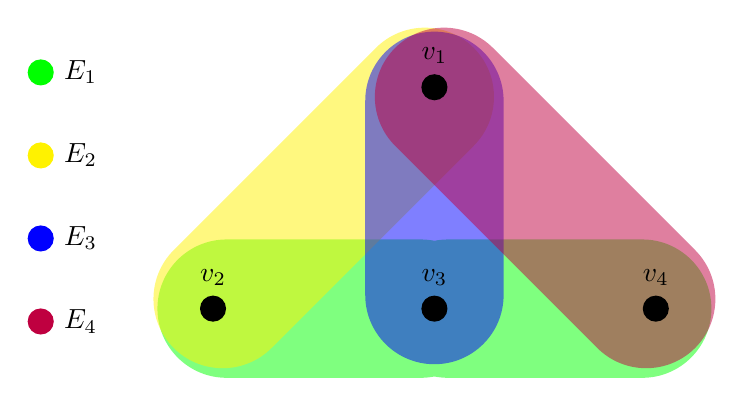
\begin{tikzpicture}
    \tikzstyle{vertex} = [fill,shape=circle,node distance=80pt]
\tikzstyle{edge} = [fill,opacity=.5,fill opacity=.5,line cap=round, line join=round, line width=50pt]
\tikzstyle{edge2} = [fill,opacity=.5,fill opacity=.5,line cap=round, line join=round, line width=40pt]
\tikzstyle{edge3} = [fill,opacity=1,fill opacity=1,line cap=round, line join=round, line width=50pt]

\tikzstyle{elabel} =  [fill,shape=circle,node distance=30pt]

\pgfdeclarelayer{background}
\pgfsetlayers{background,main}

\node[vertex,label=above:\(v_3\)] (v3) {};
\node[vertex,left of=v3,label=above:\(v_2\)] (v2) {};
\node[vertex,right of=v3,label=above:\(v_4\)] (v4) {};
\node[vertex,above of=v3,label=above:\(v_1\)] (v1) {};

\begin{pgfonlayer}{background}
\begin{scope}[transparency group,opacity=.5]
\draw[edge,opacity=1,color=green] (v2) -- (v3)--(v4);
\fill[edge,opacity=1,color=green] (v2.center)--(v3.center) -- (v4.center);
\end{scope}
\begin{scope}[transparency group,opacity=.5]
\draw[edge,opacity=1,color=yellow] (v1) -- (v2);
\fill[edge,opacity=1,color=yellow] (v1.center) -- (v2.center);
\end{scope}
\begin{scope}[transparency group,opacity=.5]
\draw[edge,opacity=1,color=blue] (v1) -- (v3);
\fill[edge,opacity=1,color=blue] (v1.center) -- (v3.center);
\end{scope}
\begin{scope}[transparency group,opacity=.5]
\draw[edge,opacity=1,color=purple] (v1) -- (v4);
\fill[edge,opacity=1,color=purple] (v1.center) -- (v4.center);
\end{scope}


\end{pgfonlayer}

\node[elabel,color=green,label=right:\(E_1\)]  (e1) at (-5,3) {};
\node[elabel,below of=e1,color=yellow,label=right:\(E_2\)]  (e2) {};
\node[elabel,below of=e2,color=blue,label=right:\(E_3\)]  (e3) {};
\node[elabel,below of=e3,color=purple,label=right:\(E_4\)]  (e4) {};

\end{tikzpicture}
\end{center}
The similarity matrix becomes:
$$S = \begin{pmatrix}
0.1566&0.2332&0.0246&0.1599&0.2332&0.1078&0.1566&0.2332\\
0.1566&0.2332&0.0246&0.1599&0.2332&0.1078&0.1566&0.2332\\
0.1566&0.2332&0.0246&0.1599&0.2332&0.1078&0.1566&0.2332\\
0.1566&0.2332&0.0246&0.1599&0.2332&0.1078&0.1566&0.2332\\
\end{pmatrix}$$
This is a beautiful example to show that sometimes (when considering easy hypergraphs), automorphic 
equivalent vertices can share the same similarity scores (see Remark 3.1.4).
\end{example}


\subsubsection{Interpretation}

\begin{itemize}
  \item[(C1)] Fulfilled: it is trivial to see that by definition of the extended 2-section, an undirected 
  graph will have exactly the same vertices and exactly the same edges in its
  extended 2-section.
    \item[(C2)] Fulfilled: the number of vertices is preserved in the extended 2-section of 
  a hypergraph, so each vertex is taken into account when calculating the 
  similarity matrix. We conclude with the same reasoning as (E2) that the 
  condition is fulfilled \textit{(equal to the `normal' 2-section)}.    
  \item[(C3)]  Fulfilled: the number of edges is preserved in the extended 2-section of 
  a hypergraph, so each edge is taken into account when calculating the 
  similarity matrix. We conclude with the same reasoning as (E3) that the 
  condition is fulfilled.
  \item[(C4)] Fulfilled: the extended 2-section preserves the adjacency relations between 
  vertices of the hypergraph by definition (namely: a vertex that is adjacent to another vertex in the hypergraph, will also be adjacent in the extended $2$-section). By preserving this relations, we can 
  use the information in (E4) to conclude that this condition is fulfilled.\textit{(equal to the `normal' 2-section)}
  \item[(C5)]   This condition does not apply on this method because we don't calculate edge similarity scores.

  \item[(C6)] Fulfilled, because:\begin{theorem}
   The extended $2$-section of a hypergraph preserves structural equivalent vertices.
  \end{theorem}
 \begin{proof}
   The structural equivalent vertices of a hypergraph $\hgraf$ form an equivalence class on the set of vertices
   $V$. Take an equivalence class $\overline{v_i}$ with $|\overline{v_i}| > 1$ (we assume that $\hgraf$ has at least two structural equivalent vertices),
   this means that all vertices in $\overline{v_i}$ have exactly the same adjacency structure in the hypegraph $\hgraf$.  
   So, when a vertex in $\overline{v_i}$ is adjacent to a vertex $v_p$ with $k$ edges that connect both vertices (the size of these
   edges doesn't matter), all 
   vertices in $\overline{v_i}$ are adjacent with $k$ edges to $v_p$ in the hypergraph 
   $\hgraf$. By the definition of the extended $2$-section, this means that all vertices 
   in $\overline{v_i}$ will also have $k$ edges connecting them to $v_p$ in the 
   $2$-section. So in the extended $2$-section, all vertices in $\overline{v_i}$ will be adjacent to 
  the same vertices, and connecting each vertex $\overline{v_i}$ with the same amount of edges to these vertices, making them also
   structural equivalent in the extended $2$-section by the definition of structural equivalent vertices in graphs.   
   
 \end{proof}
 Because the $2$-section preserves structural equivalent vertices and we use the method of Blondel for which we already proved
 in (E6) that this condition holds, the result follows.
 \textit{(equal equal to the `normal' 2-section)}   
 
  \item[(C7)] Not fulfilled: the extended 2-section doesn't save any information 
  about the number of vertices contained in an edge.
    \item[(C8)] 
     Fulfilled from the fact that isolated vertices in a hypergraph will 
  also be isolated in the extended $2$-section by definition. Because we already know from (E9) that this condition
  holds for the method of Blondel, we conclude that 
  this condition is fulfilled because the extended $2$-section preserves connectivity by definition. \textit{(equal to the `normal' 2-section)}
 \end{itemize}  
\subsubsection{Conclusion}
The extended $2$-section solves all the issues with (C1) and (C3) as it preserves all the information about the number of edges connecting
vertices 
and the adjacency of the vertices. Still, this representation is not unique as no information 
about the cardinality of the edges is saved, therefore, the method fails to (C8). Therefore, the method preforms 
much
better than the normal $2$-section, but is unreliable in detecting differences between edges. 
Still, if one is willing to accept this limitation, by example in the case of an application that 
is not focussed on detecting differences in number of vertices in th edges, the extended $2$-section can be an option.
Also note that it is impossible to calculate edge similarity scores with the extended $2$-section: 
an edge of a 
hypergraph is translated into multiple vertices in the $2$-section so it would 
be impossible to satisfy (C5) and (C7). 


\subsection{The incidence graph of a hypergraph}\index{incidence graph}\index{graph!incidence raph}\index{hypergraph representation!incidence graph}


 \subsubsection{General definitions and properties}
\begin{definition}
  Let $\hgrafeen = (V,E)$ be a hypergraph, then the \textbf{incidence graph} $\graf_i$ 
  of $\hgrafeen$ is the undirected graph with:
   
  \begin{enumerate}
    \item $V' = V \cup E$,
    \item $\forall v_i \in V, \forall E_j \in E: v_i \leftrightarrow E_j$ if $v_i \in E_j$.
      \end{enumerate}

\end{definition}
  Because all edges in $\graf_i$ are between an element of $V$ and $E$, $\grafi_i$ 
  is a bipartite graph and we write $\grafi_i = ((V,E),\leftrightarrow)$.

\begin{example}
Take the same hypergraph $\hgrafeen$ as in Example \ref{uniciteitsvoorbeeld}, 
then the incidence graph $\graf_i$ equals:
\begin{center}
\begin{tikzpicture}[<->,>=stealth',shorten >=1pt,auto,node distance=2cm,
                    thick]
                    \tikzstyle{every node}=[draw,circle,fill=black,minimum size=4pt,
                            inner sep=0pt]


  \node[main node] (1) [label=above:$v_1$] {};
  \node[main node] (2) [label=above:$v_2$][right of=1] {};
  \node[main node] (3) [label=above:$v_3$][right of=2] {};
  \node[main node] (4) [label=above:$v_4$][right of=3] {};
  \node[main node] (5) [label=above:$v_5$][right of=4] {};
  \node[main node] (6) [label=above:$v_6$][right of=5] {};
  \node[main node] (7) [label=above:$v_7$][right of=6] {};
  \node[main node] (8) [label=above:$v_8$][right of=7] {};
    \node[main node] (9) [label=below:$E_1$][below of=4] {};
    \node[main node] (10) [label=below:$E_2$][below of=5] {};
    \node[main node] (11) [label=below:$E_2$][below of=6] {};

  \path[every node/.style={font=\sffamily\small}]
   
    (3) edge node [above] {} (9)
    (4) edge node [above] {} (9)
    (4) edge node [above] {} (10)
    (1) edge node [above] {} (10)
    (2) edge node [above] {} (10)
    (5) edge node [above] {} (10)
    (7) edge node [above] {} (10)
    (8) edge node [above] {} (10)
    (2) edge node [above] {} (11)
    (5) edge node [above] {} (11)
    (6) edge node [above] {} (11)
    (8) edge node [above] {} (11)

\end{tikzpicture}
\end{center}
\end{example}
We can prove that the incidence graph $\graf_i = (W=(V,E),\leftrightarrow)$ of a hypergraph is a faitfhul 
characteristic graph representation if we know its bipartite structure.

\begin{theorem}\label{iguniek}
 The incidence graph  $\graf_i = (W=(V,E),\to)$ of a hypergraph is a faithful representation: the incidence 
 graph represents only one hypergraph under the condition that we know the 
 bipartite structure, which means that for the vertex set $W$, we know which 
 disjoint subset represents the vertices $V$ of the hypergraph, respectively the edges $E$ of the hypergraph.
\end{theorem}
\begin{proof}
  Suppose that $\hgraf$ and $\hgrafeen$ are two hypergraphs that share the same 
  incidence graph $\graf_i = ((V,E),\to)$. Then $\hgraf$ and $\hgrafeen$ have the same 
  set of vertices $V$ and the same set of edges $E$. Also the adjacency 
  relations in $\hgraf$ and $\hgrafeen$ are the same by the edge set $\to$ of 
  $\graf_i$. We conclude that $\hgraf = \hgrafeen$.
\end{proof}
\end{center} 
\subsubsection{Algorithm for similarity}
  In Listing \ref{igmatlab} in Appenix \ref{appendixa}, we introduce 
 an algorithm that 
  takes a hypergraph as input and returns the adjacency matrix of the 
  corresponding incidence graph. The 
  resulting adjacency matrix can then be used in the node similarity method from 
  Algorithm \ref{algsimilarity}.
  
  An important note has to be made here: this algorithm will return both the 
  node and edge similarity scores in the same matrix. Also similarity scores 
  will be available to compare an edge to a node and vice versa. Since we cannot give a correct meaning
  to such similarity scores, we regard them as redundant, intermediate results. In the examples, we will always draw lines
  in order to clearly separate the node similarity submatrix and the edge 
  similarity submatrix.
\subsubsection{Examples}
\begin{example}\label{igex1}
Take $\hgrafeen_1$ and $\hgrafeen_2$ as in Example \ref{ex1line}, the similarity 
matrix with the incidence graph representation becomes:
$$\left(\begin{array}{llllllll|lll}
 0.0631&0.1075&0.0101&0.0732&0.1075&0.0444&0.0631&0.1075&0.0170&0.1065&0.0748\\
0.0631&0.1075&0.0101&0.0732&0.1075&0.0444&0.0631&0.1075&0.0170&0.1065&0.0748\\
0.0129&0.0220&0.0021&0.0150&0.0220&0.0091&0.0129&0.0220&0.0035&0.0217&0.0153\\
0.0081&0.0138&0.0013&0.0094&0.0138&0.0057&0.0081&0.0138&0.0022&0.0137&0.0096\\
0.0517&0.0880&0.0082&0.0599&0.0880&0.0363&0.0517&0.0880&0.0139&0.0871&0.0612\\
0.1067&0.1817&0.0170&0.1237&0.1817&0.0750&0.1067&0.1817&0.0287&0.1799&0.1265\\
0.1067&0.1817&0.0170&0.1237&0.1817&0.0750&0.1067&0.1817&0.0287&0.1799&0.1265\\
0.0565&0.0961&0.0090&0.0655&0.0961&0.0397&0.0565&0.0961&0.0152&0.0952&0.0669\\
0.0129&0.0220&0.0021&0.0150&0.0220&0.0091&0.0129&0.0220&0.0035&0.0217&0.0153\\
0.0631&0.1075&0.0101&0.0732&0.1075&0.0444&0.0631&0.1075&0.0170&0.1065&0.0748\\
0.0631&0.1075&0.0101&0.0732&0.1075&0.0444&0.0631&0.1075&0.0170&0.1065&0.0748\\
0.0129&0.0220&0.0021&0.0150&0.0220&0.0091&0.0129&0.0220&0.0035&0.0217&0.0153\\ 
\hline
0.0123&0.0209&0.0020&0.0143&0.0209&0.0086&0.0123&0.0209&0.0033&0.0207&0.0146\\
0.0958&0.1632&0.0153&0.1111&0.1632&0.0674&0.0958&0.1632&0.0258&0.1616&0.1136\\
0.0196&0.0333&0.0031&0.0227&0.0333&0.0138&0.0196&0.0333&0.0053&0.0330&0.0232\\
0.0661&0.1126&0.0106&0.0767&0.1126&0.0465&0.0661&0.1126&0.0178&0.1115&0.0784
\end{array}\right)$$
\end{example}

\begin{example}\label{igex2}
Take $\hgrafeen_1$ and $\hgrafeen_2$ as in Example \ref{ex2line}, the similarity 
matrix with the incidence graph representation becomes:
$$\left(\begin{array}{llllllll|lll}
  0.0920&0.1566&0.0147&0.1067&0.1566&0.0647&0.0920&0.1566&0.0247&0.1551&0.1090\\
0.0920&0.1566&0.0147&0.1067&0.1566&0.0647&0.0920&0.1566&0.0247&0.1551&0.1090\\
0.0000&0.0000&0.0000&0.0000&0.0000&0.0000&0.0000&0.0000&0.0000&0.0000&0.0000\\
0.0000&0.0000&0.0000&0.0000&0.0000&0.0000&0.0000&0.0000&0.0000&0.0000&0.0000\\
0.0000&0.0000&0.0000&0.0000&0.0000&0.0000&0.0000&0.0000&0.0000&0.0000&0.0000\\
0.0920&0.1566&0.0147&0.1067&0.1566&0.0647&0.0920&0.1566&0.0247&0.1551&0.1090\\
0.0920&0.1566&0.0147&0.1067&0.1566&0.0647&0.0920&0.1566&0.0247&0.1551&0.1090\\
0.0000&0.0000&0.0000&0.0000&0.0000&0.0000&0.0000&0.0000&0.0000&0.0000&0.0000\\
0.0000&0.0000&0.0000&0.0000&0.0000&0.0000&0.0000&0.0000&0.0000&0.0000&0.0000\\
0.0920&0.1566&0.0147&0.1067&0.1566&0.0647&0.0920&0.1566&0.0247&0.1551&0.1090\\
0.0920&0.1566&0.0147&0.1067&0.1566&0.0647&0.0920&0.1566&0.0247&0.1551&0.1090\\
0.0000&0.0000&0.0000&0.0000&0.0000&0.0000&0.0000&0.0000&0.0000&0.0000&0.0000\\
\hline
0.0000&0.0000&0.0000&0.0000&0.0000&0.0000&0.0000&0.0000&0.0000&0.0000&0.0000\\
0.0920&0.1566&0.0147&0.1067&0.1566&0.0647&0.0920&0.1566&0.0247&0.1551&0.1090\\
0.0000&0.0000&0.0000&0.0000&0.0000&0.0000&0.0000&0.0000&0.0000&0.0000&0.0000
\end{array}\right)$$

\end{example}

\begin{example}\label{igex3}
Take $\hgrafeen_1$ and $\hgrafeen_2$ as in Example \ref{ex3line}, the similarity 
matrix with the incidence graph representation becomes:
$$\left(\begin{array}{llllllll|lll}
0.0839&0.1428&0.0134&0.0972&0.1428&0.0589&0.0839&0.1428&0.0226&0.1414&0.0994\\
0.0839&0.1428&0.0134&0.0972&0.1428&0.0589&0.0839&0.1428&0.0226&0.1414&0.0994\\
0.0000&0.0000&0.0000&0.0000&0.0000&0.0000&0.0000&0.0000&0.0000&0.0000&0.0000\\
0.0254&0.0432&0.0041&0.0294&0.0432&0.0178&0.0254&0.0432&0.0068&0.0428&0.0301\\
0.0254&0.0432&0.0041&0.0294&0.0432&0.0178&0.0254&0.0432&0.0068&0.0428&0.0301\\
0.1092&0.1860&0.0174&0.1267&0.1860&0.0768&0.1092&0.1860&0.0294&0.1842&0.1295\\
0.0839&0.1428&0.0134&0.0972&0.1428&0.0589&0.0839&0.1428&0.0226&0.1414&0.0994\\
0.0000&0.0000&0.0000&0.0000&0.0000&0.0000&0.0000&0.0000&0.0000&0.0000&0.0000\\
0.0000&0.0000&0.0000&0.0000&0.0000&0.0000&0.0000&0.0000&0.0000&0.0000&0.0000\\
0.0839&0.1428&0.0134&0.0972&0.1428&0.0589&0.0839&0.1428&0.0226&0.1414&0.0994\\
0.0839&0.1428&0.0134&0.0972&0.1428&0.0589&0.0839&0.1428&0.0226&0.1414&0.0994\\
0.0000&0.0000&0.0000&0.0000&0.0000&0.0000&0.0000&0.0000&0.0000&0.0000&0.0000\\
\hline
0.0302&0.0514&0.0048&0.0350&0.0514&0.0212&0.0302&0.0514&0.0081&0.0509&0.0358\\
0.0997&0.1697&0.0159&0.1156&0.1697&0.0701&0.0997&0.1697&0.0268&0.1681&0.1181\\
0.0000&0.0000&0.0000&0.0000&0.0000&0.0000&0.0000&0.0000&0.0000&0.0000&0.0000
\end{array}\right)
\end{eqnarray*}

\end{example}
\begin{example}\label{igex4}
Take $\hgrafeen_1$ and $\hgrafeen_2$ as in Example \ref{ex4line}, the similarity 
matrix with the incidence graph representation becomes:
\begin{eqnarray*}
  \left(\begin{array}{llllllll|lll}
0.0565&0.0961&0.0090&0.0655&0.0961&0.0397&0.0565&0.0961&0.0152&0.0952&0.0669\\
0.0944&0.1608&0.0151&0.1095&0.1608&0.0664&0.0944&0.1608&0.0254&0.1592&0.1119\\
0.0253&0.0431&0.0040&0.0293&0.0431&0.0178&0.0253&0.0431&0.0068&0.0427&0.0300\\
0.0818&0.1392&0.0130&0.0948&0.1392&0.0575&0.0818&0.1392&0.0220&0.1379&0.0969\\
0.0944&0.1608&0.0151&0.1095&0.1608&0.0664&0.0944&0.1608&0.0254&0.1592&0.1119\\
0.0379&0.0646&0.0061&0.0440&0.0646&0.0267&0.0379&0.0646&0.0102&0.0640&0.0450\\
0.0565&0.0961&0.0090&0.0655&0.0961&0.0397&0.0565&0.0961&0.0152&0.0952&0.0669\\
0.0944&0.1608&0.0151&0.1095&0.1608&0.0664&0.0944&0.1608&0.0254&0.1592&0.1119\\
\hline
0.0237&0.0403&0.0038&0.0275&0.0403&0.0166&0.0237&0.0403&0.0064&0.0399&0.0281\\
0.1057&0.1800&0.0169&0.1226&0.1800&0.0743&0.1057&0.1800&0.0284&0.1783&0.1253\\
0.0710&0.1210&0.0113&0.0824&0.1210&0.0499&0.0710&0.1210&0.0191&0.1198&0.0842\\
0.0237&0.0403&0.0038&0.0275&0.0403&0.0166&0.0237&0.0403&0.0064&0.0399&0.0281
\end{array}\right)$$

\end{example}
\begin{example}\label{igex5}
  Take $\hgraf_1$ and $\hgraf_2$ as in Example \ref{ex2extended}, the similarity 
  matrix becomes:
$$\left(\begin{array}{llllllll|lll}
  0.1034&0.1761&0.0165&0.1199&0.1761&0.0727&0.1034&0.1761&0.0278&0.1744&0.1226\\
0.0794&0.1352&0.0127&0.0921&0.1352&0.0558&0.0794&0.1352&0.0214&0.1339&0.0941\\
0.0794&0.1352&0.0127&0.0921&0.1352&0.0558&0.0794&0.1352&0.0214&0.1339&0.0941\\
0.0794&0.1352&0.0127&0.0921&0.1352&0.0558&0.0794&0.1352&0.0214&0.1339&0.0941\\
\hline
0.1034&0.1761&0.0165&0.1199&0.1761&0.0727&0.1034&0.1761&0.0278&0.1744&0.1226\\
0.0794&0.1352&0.0127&0.0921&0.1352&0.0558&0.0794&0.1352&0.0214&0.1339&0.0941\\
0.0794&0.1352&0.0127&0.0921&0.1352&0.0558&0.0794&0.1352&0.0214&0.1339&0.0941\\
0.0794&0.1352&0.0127&0.0921&0.1352&0.0558&0.0794&0.1352&0.0214&0.1339&0.0941
\end{array}\right)$$
\end{example}

\subsubsection{Interpretation}

\begin{itemize}
  \item[(C1)] Fulfilled: we will prove later in Corallary \ref{gelijktjekdj} 
  that using this method with two undirected graphs returns the same results as 
  the node-edge similarity matrix of section 2.3.
      \item[(C2)] Fulfilled: the number of vertices is preserved in the incidence graph a hypergraph, so each vertex is taken into account when calculating the similarity matrix. We conclude with the same reasoning as (E2) that the condition is fulfilled.
    \item[(C3)] Fulfilled from the fact that all edges are 
    represented in the incidence graph of the hypergraph, so each edge is taken into account when calculating the similarity matrix. We conclude with the same reasoning as (E3) that the condition is fulfilled.

  \item[(C4)] Fulfilled from the fact that the adjacency relations of the original hypergraph are represented in its 
  incidence graph and that we use Algorithm \ref{algsimilarity}, for which this 
  statement already holds by (E4).
  
  An example can be found in Example \ref{igex1} where $v_2, v_5, v_8$ of $\hgrafeen_1$ 
  have the largest similarity score with $v_6, v_7$ of $\hgrafeen_2$. This is 
  not surprising as $v_6, v_7$ are contained in all possible edges.
  \item[(C5)] Fulfilled from the fact that the adjacency relations of the original hypergraph are represented in its 
  incidence graph, that the edges are considered as normal vertices and that we use Algorithm \ref{algsimilarity}, for which this 
  statement already holds by (E4).
  
  
  An example can be found in Example \ref{igex1} where $E_2$ of $\hgrafeen_1$ 
  has the largest similarity score with $E'_2$ of $\hgrafeen_2$. This is 
  not surprising as these edges are almost equal.


  \item[(C6)] Fulfilled, an example of structural equivalent edges can be found in Example \ref{igex4}, where 
  $E'_1$ and $E'_4$ of $\hgrafeen_2$ have the same similarity scores. In the same 
  example, the vertices $v_1, v_7$ of $\hgrafeen_2$ as well as $v_2, v_5, v_8$.

We know prove that the incidence graph preserves the interchangeability of edges and 
vertices:
\begin{theorem}
   The incidence graph of a hypergraph preserves structural equivalent vertices. \end{theorem}
 \begin{proof}
   The structural equivalent vertices of a hypergraph $\hgraf$ form an equivalence class on the set of vertices
   $V$, take an equivalence $\overline{v_i}$ with $|\overline{v_i}| > 1$ (we assume that $\hgraf$ has at least two structural equivalent vertices),
   this means that all vertices in $\overline{v_i}$ have exactly the same adjacency structure in the hypegraph $\hgraf$.  
   So, when a vertex in $\overline{v_i}$ is adjacent to a vertex $v_p$, all 
   vertices in $\overline{v_i}$ are adjacent with the same edge $E_k$ to $v_p$ in the hypergraph 
   $\hgraf$. By the definition of the incidence graph, this means that all vertices in 
   in $\overline{v_i}$ will be connected to the edge $E_k$ connecting them to $v_p$ in the 
   incidence graph.  So in the incidence graph, all vertices in $\overline{v_i}$ will be adjacent to 
  the same vertices and the same edges, making them also structural equivalent by the definition of structural equivalent vertices in graphs. With the same reasoning, we conlcude
  that also the structural equivalent edges are preserved.  
   
 \end{proof}



  \item[(C7)] Fulfilled: the adjancency relations in the incidence graph are determined by the number of vertices
  contained in an edge in the hypergraph.
    \item[(C8)] Fulfilled. An example is Example \ref{ex3line} where the 
    vertices $v_3, v_8, v_9$ and $v_12$ have all similarity scores equal to zero 
    as they form a clique that is not connected to the other vertices. The 
    incidence graph also preserves the adjancency relations and thus 
    connectivity, so we know from (E8) that this condition holds.
  \end{itemize}  
  \subsubsection{Conclusion}
  We conclude that using the incidence graph returns similarity scores that 
  satisfy all the conditions and can be seen as a very good way to calculate the 
  similarity scores of a hypergraph. By Theorem \ref{iguniek} this is not so 
  surprising: the incidence graph is a faithful representation. Intuitively, 
  this means that this representation saves all information of the represented 
  hypergraph, meaning that it is possible to reconstruct the hypergraph based on 
  its incidece graph. As a result, no information of the hypergraph is lost when using Algorithm \ref{algsimilarity},
  so it is possible to satisfy all the conditions. 

\newpage
  \section{Similarity by using the incidence matrix}\index{incidence matrix}\index{graph!incidence matrix}\index{hypergraph representation!incidence matrix}

We already showed that using the incidence graph representation of a hypergraph
is a very good way to calculate similarity between hypergraphs. It would be somehow logic to stop searching for similarity methods
for hypergraphs now, but there is one very natural generalization that is worth mentioning: the node-edge similarity 
method described in Section 2.3 uses a source-edge matrix and a terminus-edge 
matrix. When we would use this method (see Theorem \ref{edgegrootbewijs}) with undirected graphs $\graf$ and $\grafeen$, the source-edge matrix and terminus-edge
matrix are the same and are equal to the \textit{incidence matrices} of $\graf$ and 
$\grafeen$. The question is now: is there any problem if we enter not the incidence matrices of two graphs, but of 
two hypergraphs (see Definition \ref{incidencematrixhypergraph})? The only difference is that each
column can have more than 2 entries equal to 1. The answer is 
no. 

Even better, we will be able to prove that this method is equal to the method with the incidence graph up to a 
constant! By this `concluding theorem', we know that also this methods meets all 
conditions imposed in the introduction. 

We first prove the compact form of the method:

\subsection{Compact form}
 \begin{theorem}\label{incidencegrootbewijs}
   Let $\hgraf=(V,E)$ and $\hgrafeen=(V',E')$ be two hypergraphs, $\hgraf$ has $n_\hgraf$ 
   vertices and $m_\hgraf$ eges and $\hgrafeen$ has $n_\hgrafeen$ vertices and $m_\hgrafeen$ 
   edges. Let $A$ and $B$ be the incidence matrices of $\hgraf$ and $\hgrafeen$ 
   and define:
 \begin{eqnarray}
  Y^{(k+1)} &=& \frac{B^TX^{(k)}A}{\|B^TX^{(k)}A\|_F}\label{edgehypform}\\
   X^{(k+1)} &=& \frac{BY^{(k)}A^T}{\|BY^{(k)}A^T\|_F}\label{nodehypform}
 \end{eqnarray}
  for  $k =  0,1,\ldots$.
  
  Then the matrix subsequences $X^{(2k)}$, $Y^{(2k)}$ and $X^{(k+1)}$, $Y^{(k+1)}$ 
  converge to $X_{\text{even}}$, $Y_{\text{even}}$ and $X_{\text{odd}}$, 
  $Y_{\text{odd}}$. If we take:
  \begin{eqnarray*}  X^{(0)} = J \in \R^{n_\grafeen \times n_\graf}\\
    Y^{(0)} = J \in \R^{m_\grafeen \times m_\graf}
  \end{eqnarray*}
 as initial matrices, then $X_{\text{even}}(J)=X_{\text{odd}}(J)$, $Y_{\text{even}}(J)= Y_{\text{odd}}(J)$ 
 are the unique matrices of largest 1-norm among all possible limits with positive 
 initial matices and the matrix sequence $X^{(k)}$, $Y^{(k)}$ converges has a 
 whole.
  \end{theorem}
  \begin{proof}
 The only thing we have to prove is that we can construct a matrix $M$ that is 
 nonnegative and symmetric, the rest of the proof is completely analogous to the proof of Theorem 
 \ref{edgegrootbewijs}.
 
 So, by Theorem \ref{tensor} we can rewrite (\ref{edgematrix1}) as follows:
 \begin{eqnarray*}
         Y'^{(k+1)} &=& B^TX^{(k)}A\\
  \Leftrightarrow  \vect(Y'^{(k+1)}) &=& \vect(B^TX'^{(k)}A)\\
  \Leftrightarrow  \vect(Y'^{(k+1)}) &=& (A^T \otimes B^T)\vect(X'^{(k)})
   \end{eqnarray*}
 Completely analogous we can also rewrite (\ref{edgematrix2}):
 $$\vect(X'^{(k+1)}) &=& (A \otimes B)\vect(Y'^{k}),$$
 define $\mathbf{y}^{(k)}=\vect(Y'^{(k+1)})$ and $\mathbf{x}^{(k)}= \vect(X'^{(k+1)})$, we get:
 \begin{eqnarray*}
   \mathbf{y}^{(k+1)} &=& (A^T \otimes B^T)\mathbf{x}^{(k)}\\
   \mathbf{x}^{(k+1)} &=& (A \otimes B)\mathbf{y}^{(k)}
 \end{eqnarray*} 
 If we define $G = A^T \otimes B^T$, then with Lemma \ref{hulptensor}:
  \begin{eqnarray*}
   G^T &=& (A^T \otimes B^T)^T\\
   &=& A \otimes B \end{eqnarray*}
 So we get:
  \begin{eqnarray}
     \mathbf{y}^{(k+1)} &=& G\mathbf{x}^{(k)}\label{uitgeschrevenvectoren1}\\
     \mathbf{x}^{(k+1)} &=& G^T\mathbf{y}^{(k)}\label{uitgeschrevenvectoren2},
 \end{eqnarray}
$G$ is a $m_\graf m_\grafeen \times n_\graf n_\grafeen$-matrix, the previous expressions  can be concatenated to a single matrix update equation (we define matrix $M$ and $\mathbf{z}^{(k+1)}$):
 $$\mathbf{z}^{(k+1)} =\begin{pmatrix}
 \mathbf{x}\\
 \mathbf{y}
 \end{pmatrix}^{(k+1)} = \begin{pmatrix}
 0_{m_\graf m_\grafeen} & G^T\\
 G & 0_{n_\graf n_\grafeen} \\
 \end{pmatrix}
 \begin{pmatrix}
 \mathbf{x}\\
 \mathbf{y}
 \end{pmatrix}^{(k)}
 = M\mathbf{z}^{(k)},$$
  M is clearly nonnegative because $G$ and $G^T$ are nonnegative and $M$ is also
 clearly symmetric, so the result follows immediately from Theorem \ref{grootbewijs}. 
The rest of the proof is now completely analogous to the proof of Theorem 
\ref{edgegrootbewijs}.

 \end{proof}
 We define now $X_{\text{even}}(\mathbf{1})$ as the node similarity matrix and $Y_{\text{even}}(\mathbf{1})$ as the edge similarity 
 matrix.
 
 Note that the equations in compact form in the node-edge similarity method 
 where defined as:
  \begin{eqnarray*}
  Y^{(k+1)} &=& \frac{B_S^TX^{(k)}A_S + B_T^TX^{(k)}A_T}{\|B_S^TX^{(k)}A_S + 
  B_T^TX^{(k)}A_T\|_F}\\
   X^{(k+1)} &=& \frac{B_SY^{(k)}A_S^T + B_TY^{(k)}A^T_T}{\|B_SY^{(k)}A_S^T + 
   B'_TY^{(k)}A^T_T\|_F}
 \end{eqnarray*}
 
 But since $A_S = A_T = A$ and $B_S = B_T = B$ in this case, the second term of the sum is redundant 
and would be eliminated by the normalization in each step. This shows that the 
compact form as presented in the previous theorem is not different from the 
compact form of Theorem \ref{edgegrootbewijs}.

\subsection{The algorithm}
The algorithm is completely analogous to Algorithm 6. A Matlab implementation 
can be found in Listing \ref{edgealgorithmhypergraphmatlab} in Appendix 
\ref{appendixa}. We also present Algorithm \ref{incidencealg}, an algorithm that 
takes a hypergraph as input and returns the incidence matrix of the hypergraph. A Matlab implementation of this algorithm
can be found in Listing A.15.


\begin{algorithm}[H]\label{edgealgorithmhypergraph}
 \KwData{\\
 $A$:  the $n_\hgraf \times m_\hgraf$ incidence matrix of a hypergraph $\hgraf$\\
 $B$: the $n_\hgrafeen \times m_\hgrafeen$ incidence matrix of a hypergraph $\hgraf$\\
 $\tol$: tolerance for the estimation error.\\
 \KwResult{\\
 $X$: the node similarity matrix between $\graf$ and $\grafeen$\\
 $Y$: the edge similarity matrix between $\graf$ and $\grafeen$}
 \blankline
\SetKwFunction{powermethod}{node\_edge\_similarity\_matrix\_hypergraphs}
\SetKwFunction{hits}{hits}

\SetKwProg{myalg}{begin}{}{end}
\myalg{\powermethod{$A$,$B$,$\tol$}}{
$k = 1$ \;
$X^{(0)} = \mathbf{1}$ ($n_\grafeen\times n_\graf$-matrix with all entries equal to $1$)\;
$Y^{(0)} = \mathbf{1}$ ($m_\grafeen\times m_\graf$-matrix with all entries equal to $1$)\;
$\mu_X =  n_\grafeen\times n_\graf$-matrix with all entries equal to $\tol$\;
$\mu_Y =  m_\grafeen\times m_\graf$-matrix with all entries equal to $\tol$\;

\Repeat{$|X^{(k)} - X^{(k-1)}| < \mu_X$ and $|Y^{(k)} - Y^{(k-1)}| < \mu_Y$ }{
$Y^{(k)}=& \frac{B^TX^{(k-1)}A}{\|B^TX^{(k-1)}A\|_F}$\;
$X^{(k)} = \frac{BY^{(k)}A^T}{\|BY^{(k)}A^T\|_F}$\;
$k = k + 1$\;
}}
 
\KwRet $X^{(k)}, Y^{(k)} $\;}{}
  \caption{Algorithm for calculating the node and edge similarity matrix $X$ and $Y$ between $\hgraf$ and $\hgrafeen$.\\}
  \end{algorithm}
  
  \begin{algorithm}[H]\label{incidencealg}
 \KwData{\\
 $n$:  the number of vertices of hypergraph $\hgrafeen$\\
 $E$:  a set of subsets $E_i$ of $\{1, \ldots, n\}$ that represent the edges of hypergraph $\hgrafeen$\\}
 \KwResult{\\
 $A$: the incidence matrix of the hypergraph}
 \blankline
\SetKwFunction{powermethod}{hypergraph\_to\_incidencematrix}
\SetKwFunction{hits}{hits}

\SetKwProg{myalg}{begin}{}{end}
\myalg{\powermethod{$n$, $E$}}{
$m = |E|$\;
$A$ = initialize a $n \times n$-matrix with all entries equal to 0\;

\For{$E_j \in E$ }{
  \For{$v_i \in E_j$}{
    $(A)_{ij} = 1$\;
  }}
\KwRet $A$\;}{}
  \caption{Algorithm to calculate the adjacency matrix of the 2-section of a hypergraph.\\}
\end{algorithm}
\subsection{Examples}
We now calculate the same example as in the previous section:

\begin{example}
  Let $\hgrafeen_1$, $\hgrafeen_2$ be the same hypergraphs as in Example \ref{ex1line}, we get as incidence matrix $A$ of 
  $\hgrafeen_1$ and $B$ of $\hgrafeen_2$:
  $$A = \begin{pmatrix}
  0&1&0\\
0&1&1\\
1&0&0\\
1&1&0\\
0&1&1\\
0&0&1\\
0&1&0\\
0&1&1\\
\end{pmatrix} \quad \text{and} \quad
B = \begin{pmatrix}
  0&1&0&0\\
0&1&0&0\\
0&0&1&0\\
1&0&0&0\\
1&0&0&1\\
0&1&0&1\\
0&1&0&1\\
0&0&1&1\\
0&0&1&0\\
0&1&0&0\\
0&1&0&0\\
0&0&1&0
\end{pmatrix}$$
which can be used to apply Algorithm \ref{edgealgorithmhypergraph} which results in the node similarity matrix $X$ and the edge similarity matrix 
$Y$:
$$ X = \begin{pmatrix}
0.0838&0.1428&0.0134&0.0972&0.1428&0.0589&0.0838&0.1428\\
0.0838&0.1428&0.0134&0.0972&0.1428&0.0589&0.0838&0.1428\\
0.0171&0.0291&0.0027&0.0198&0.0291&0.0120&0.0171&0.0291\\
0.0108&0.0183&0.0017&0.0125&0.0183&0.0076&0.0108&0.0183\\
0.0686&0.1168&0.0109&0.0796&0.1168&0.0482&0.0686&0.1168\\
0.1417&0.2413&0.0226&0.1643&0.2413&0.0996&0.1417&0.2413\\
0.1417&0.2413&0.0226&0.1643&0.2413&0.0996&0.1417&0.2413\\
0.0750&0.1277&0.0120&0.0869&0.1277&0.0527&0.0750&0.1277\\
0.0171&0.0291&0.0027&0.0198&0.0291&0.0120&0.0171&0.0291\\
0.0838&0.1428&0.0134&0.0972&0.1428&0.0589&0.0838&0.1428\\
0.0838&0.1428&0.0134&0.0972&0.1428&0.0589&0.0838&0.1428\\
0.0171&0.0291&0.0027&0.0198&0.0291&0.0120&0.0171&0.0291
\end{pmatrix}$$
$$Y = \begin{pmatrix}
0.0134&0.0840&0.0590\\
0.1045&0.6549&0.4603\\
0.0213&0.1337&0.0940\\
0.0721&0.4519&0.3177
\end{pmatrix}$$
\end{example}

\begin{example}
  Take $\hgrafeen_1$ and $\hgrafeen_2$ as in Example \ref{ex2line}, the node 
  similarity matrix $X$ and the edge similarity matrix $Y$ become:
  $$X=\begin{pmatrix}
    0.1152&0.1961&0.0184&0.1336&0.1961&0.0810&0.1152&0.1961\\
0.1152&0.1961&0.0184&0.1336&0.1961&0.0810&0.1152&0.1961\\
0.0000&0.0000&0.0000&0.0000&0.0000&0.0000&0.0000&0.0000\\
0.0000&0.0000&0.0000&0.0000&0.0000&0.0000&0.0000&0.0000\\
0.0000&0.0000&0.0000&0.0000&0.0000&0.0000&0.0000&0.0000\\
0.1152&0.1961&0.0184&0.1336&0.1961&0.0810&0.1152&0.1961\\
0.1152&0.1961&0.0184&0.1336&0.1961&0.0810&0.1152&0.1961\\
0.0000&0.0000&0.0000&0.0000&0.0000&0.0000&0.0000&0.0000\\
0.0000&0.0000&0.0000&0.0000&0.0000&0.0000&0.0000&0.0000\\
0.1152&0.1961&0.0184&0.1336&0.1961&0.0810&0.1152&0.1961\\
0.1152&0.1961&0.0184&0.1336&0.1961&0.0810&0.1152&0.1961\\
0.0000&0.0000&0.0000&0.0000&0.0000&0.0000&0.0000&0.0000
  \end{pmatrix}$$
  
    $$Y=\begin{pmatrix}
    0.0000&0.0000&0.0000\\
0.1294&0.8112&0.5702\\
0.0000&0.0000&0.0000
  \end{pmatrix}$$
  

\end{example}

\begin{example}
  Take $\hgrafeen_1$ and $\hgrafeen_2$ as in Example \ref{ex3line}, the node 
  similarity matrix $X$ and the edge similarity matrix $Y$ become:
  $$X=\begin{pmatrix}
    0.1076&0.1832&0.0172&0.1247&0.1832&0.0756&0.1076&0.1832\\
0.1076&0.1832&0.0172&0.1247&0.1832&0.0756&0.1076&0.1832\\
0.0000&0.0000&0.0000&0.0000&0.0000&0.0000&0.0000&0.0000\\
0.0326&0.0555&0.0052&0.0378&0.0555&0.0229&0.0326&0.0555\\
0.0326&0.0555&0.0052&0.0378&0.0555&0.0229&0.0326&0.0555\\
0.1401&0.2386&0.0224&0.1625&0.2386&0.0985&0.1401&0.2386\\
0.1076&0.1832&0.0172&0.1247&0.1832&0.0756&0.1076&0.1832\\
0.0000&0.0000&0.0000&0.0000&0.0000&0.0000&0.0000&0.0000\\
0.0000&0.0000&0.0000&0.0000&0.0000&0.0000&0.0000&0.0000\\
0.1076&0.1832&0.0172&0.1247&0.1832&0.0756&0.1076&0.1832\\
0.1076&0.1832&0.0172&0.1247&0.1832&0.0756&0.1076&0.1832\\
0.0000&0.0000&0.0000&0.0000&0.0000&0.0000&0.0000&0.0000
  \end{pmatrix}$$
  
    $$Y=\begin{pmatrix}
    0.0375&0.2351&0.1652\\
0.1239&0.7764&0.5457\\
0.0000&0.0000&0.0000
  \end{pmatrix}$$
  

\end{example}
\begin{example}
  Take $\hgrafeen_1$ and $\hgrafeen_2$ as in Example \ref{ex4line}, the node 
  similarity matrix $X$ and the edge similarity matrix $Y$ become:
  $$X=\begin{pmatrix}
  0.0778&0.1326&0.0124&0.0903&0.1326&0.0547&0.0778&0.1326\\
0.1302&0.2216&0.0208&0.1509&0.2216&0.0915&0.1302&0.2216\\
0.0349&0.0594&0.0056&0.0404&0.0594&0.0245&0.0349&0.0594\\
0.1127&0.1919&0.0180&0.1307&0.1919&0.0792&0.1127&0.1919\\
0.1302&0.2216&0.0208&0.1509&0.2216&0.0915&0.1302&0.2216\\
0.0523&0.0891&0.0083&0.0607&0.0891&0.0368&0.0523&0.0891\\
0.0778&0.1326&0.0124&0.0903&0.1326&0.0547&0.0778&0.1326\\
0.1302&0.2216&0.0208&0.1509&0.2216&0.0915&0.1302&0.2216
  \end{pmatrix}$$
  
    $$Y=\begin{pmatrix}
0.0233&0.1459&0.1025\\
0.1039&0.6512&0.4577\\
0.0698&0.4376&0.3076\\
0.0233&0.1459&0.1025
  \end{pmatrix}$$
  

\end{example}
 \subsection{Concluding theorem}
 Before heading to an interpretation of the examples and the method, we now 
 present a `concluding theorem' that shows that the method of similarity using 
 the incidence matrix is completely equal to the method with the incidence graph 
 of the matrix. This gives us an immediate guarantee that all conditions of the 
 introduction are met for the method with the incidence matrix.
\begin{theorem}\label{concludingtheorem}
  The similarity method using the incidence graphs of two hypergraphs $\hgraf, \hgrafeen$ returns the same results as the method with the 
  incidence matrices of $\hgraf, \hgrafeen$, up to a constant, so:
\begin{eqnarray*}
  X^{(k)} &=& \alpha S^{(k)}[1,\ldots,n_\hgrafeen;1,\ldots,n_\hgraf]\\
  Y^{(k)} &=& \beta S^{(k)}[n_\hgrafeen,\ldots, m_\hgrafeen;n_\hgraf,\ldots, m_\hgraf]
\end{eqnarray*}
with $X, Y$, the node and similarity matrices of the method with the incidence matrices of $\hgrafeen, \hgraf$, $S$ the 
similarity matrix of method of Blondel used with the incidence graphs of $\hgrafeen, \hgraf$ 
and $\alpha, \beta \in \R$ and $k$ even. $S[R,C]$ denotes the submatrix of $S$ with rows $R$
 and columns $C$. \end{theorem}\index{submatrix}
 \begin{proof}
To calculate the similarity matrix using the incidence graph representation with the method of Blondel, an element $s_{ij}$ at iteration step $k$ is calculated as follows
(remember that $A, B$ are symmetric):
\begin{eqnarray}\label{simisimi}
s^{(k+1)}_{ij} = \frac{\sum^{n_\hgrafeen + m_\hgrafeen}_{f=1}\sum^{n_\hgraf + m_\hgraf}_{g=1} b_{if}s^{(k)}_{fg}a_{gj}}{\|BS^{(k)}A^T\|_F}
\end{eqnarray}
Now, remember that the incidence graph is a bipartite graph and thus, the 
adjancecy matrices A and B have the following property (remember our convention to order the columns and rows in a way that the vertices come first, followed by the edges):
\begin{eqnarray}\label{nulpoints}
b_{if} = 0  &\text{when }& 0 \leq i,f \leq n_\hgrafeen \text{ or } n_\hgrafeen \leq i,f \leq n_\hgrafeen + 
m_\hgrafeen\\
a_{gj} = 0  &\text{when }& 0 \leq g,j \leq n_\hgraf \text{ or } n_\hgraf \leq g,j \leq n_\hgraf + m_\hgraf
\end{eqnarray}
We are only interested in the case where $s_{ij}$ is a calculation between nodes 
and between edges, as the method with the incidence matrix also only calculates 
this and it is rather hard to give a correct meaning to a comparision between an 
edge and an a node. 

For the rest of the proof, we only consider the calculating of node similarity, the calculation 
of edge similarity is completely analogous. In this case, we have that $0 \leq i \leq n_\hgrafeen$
 and $0 \leq j \leq n_\hgraf$, now (\ref{simisimi}) becomes with property 
 (\ref{nulpoints}):
\begin{eqnarray}s^{(k+1)}_{ij} = \frac{\sum^{n_\hgrafeen + m_\hgrafeen}_{f=n_\hgrafeen}\sum^{n_\hgraf + m_\hgraf}_{g=n_\hgraf} 
b_{if}s^{(k)}_{fg}a_{gj}}{\|BS^{(k)}A^T\|_F}\label{nulnul}\end{eqnarray}
So in the case of calculating similarities between nodes, only the $s_{ij}^{(k)}$ of 
the edges play a role! Now, remember the compact form with the method using the incidence 
matrices ($B'$ is the incidence matrix of $\hgrafeen$, $A'$ of $\hgraf$, the rows in the incidence graph
represent the vertices, the columns the edges):
 \begin{eqnarray}
   X^{(k+1)} &=& \frac{B'Y^{(k)}A'^T}{\|B'Y^{(k)}A'^T\|_F}\\
     Y^{(k+1)} &=& \frac{B'^TX^{(k)}A'}{\|B'^TX^{(k)}A'\|_F}
 \end{eqnarray}
 Elementwise, we write:
 \begin{eqnarray}
  x^{(k+1)}_{ij} &=& \frac{\sum^{m_\hgrafeen}_{p=1}\sum^{m_\hgraf}_{q=1} b'_{ip}y^{(k)}_{pq}a'_{jq}}{\|B'^TX^{(k)}A'\|_F}\label{ikmoetgelijkzijn}\\
  y^{(k+1)}_{cd} &=& \frac{\sum^{n_\hgrafeen}_{h=1}\sum^{n_\hgraf}_{e=1} b'_{hc}x^{(k)}_{he}a'_{ed}}{\|B'Y^{(k)}A'^T\|_F}
 \end{eqnarray}
 Now every non-zero element of the adjacency matrices $A, B$, can be found in the 
 incidence matrices $A', B'$ too (we assume that the vertices and edges have the same numbering in both 
 matrices):
 $$ a_{ij} = \begin{cases} a'_{i,j-n_\hgrafeen} &\text{if } 0\leq i \leq n_\hgrafeen  \text{ and } n_\hgrafeen < j \leq n_\hgrafeen + m_\hgrafeen\\ 
a'_{j,i-n_\hgrafeen} & \text{if } n_\hgrafeen < i \leq n_\hgrafeen + m_\hgrafeen \text{ and } 0 \leq j \leq n_\hgrafeen\end{cases} $$
So we rewrite \ref{nulnul} an we get (remember that $0 \leq i \leq n_\hgrafeen$
 and $0 \leq j \leq n_\hgraf$):
\begin{eqnarray}
  s^{(k+1)}_{ij} &=& \frac{\sum^{n_\hgrafeen + m_\hgrafeen}_{f=n_\hgrafeen}\sum^{n_\hgraf + m_\hgraf}_{g=n_\hgraf} 
b'_{i,f-n_\hgrafeen}s^{(k)}_{fg}a'_{j,g-n_\hgraf}}{\|BS^{(k)}A^T\|_F}\\
 &=& \frac{\sum^{m_\hgrafeen}_{f=1}\sum^{m_\hgraf}_{g=1} 
b'_{i,f}s^{(k)}_{f+n_\hgrafeen,g+n_\hgraf}a'_{j,g}}{\|BS^{(k)}A^T\|_F}\label{gelijkheidjeknallen}
\end{eqnarray}
The equivalence of (\ref{gelijkheidjeknallen}) and (\ref{ikmoetgelijkzijn}) is 
now clear: (\ref{gelijkheidjeknallen}) depends on the edge similarity scores (to 
calculate the node similarity scores) and every edge similarity score is 
multiplied with exactly the same entries of the incidence graph. The result 
follows by proving that also the edge similarity scores $y_{cd}$ are equal to 
the $s_{ij}$ with $n_\hgrafeen < i \leq n_\hgrafeen + m_\hgrafeen$ and $n_\hgraf < j \leq n_\hgraf + 
m_\hgraf$, this is possible with the exact same reasoning. The difference up to 
a constant is caused by the normalization in each iteration. We conclude that 
the theorem is true for each even $k$.
 \end{proof}

 \begin{corollary}\label{gelijktjekdj}
   The node-edge similarity method (see 2.3) returns the same results for undirected graphs $\graf, \grafeen$ as
   the node similarity method of Blondel (see 2.1) using incidence graphs of $\graf, \grafeen$, up to constant. 
 \end{corollary}

\begin{proof}
  This follows immediately from the fact that in the node-edge similarity method 
  for undirected graphs, the source-edge matrix and terminal-edge matrix are the 
  same and are both equal to the incidence matrix for undirected graphs (see Definition \ref{incidencematrixgraph}).
\end{proof}
 
 \begin{remark}
   One may wonder whether the node-edge similarity method of 2.3 also returns 
   the same results for directed graphs $\graf, \grafeen$ as the node similarity 
   method of Blondel using the incidence graphs of $\graf, \grafeen$. This is the case, but is a 
   little harder to prove. First, we use the following definition for the incidence graph of a directed graph:
    \begin{definition}\index{incidence graph}\index{graph!incidence graph}
  Let $\graf = (V,\to)$ be a directed graph, then the \textbf{incidence graph} $\graf'_i =(V', \to')$ 
  of $\graf$ is the directed graph with:
   
  \begin{enumerate}
    \item $V' = V \cup \to$,
    \item $\forall v_i \in V, \forall e_j \in \to: v_i \to e_j$ if $v_i$ is the source node of $e_j$,
    \item $\forall v_i \in V, \forall e_j \in \to: e_j \to v_i$ if $v_i$ is the terminal node of $e_j$.
 \end{enumerate}

\end{definition}
  Starting from the node-edge similarity method described in section 2.3,
   we notice that this method uses source-edge and terminal-edge matrices. In 
   the undirected case, the source-edge and terminal-edge of a graph are both equal to the 
   incidence matrix of the graph, but this is not true for the directed case. Indeed, both 
   the source-edge and the terminal-edge matrix have nonnegative entries and therefore the node-edge similarity method returns nonnegative
   (node or edge) similarity scores, while the incidence matrix for directed graphs also contains negative entries (see Definition 
   \ref{incidencematrixgraph}).  Still, we can prove that using the method of 
   Blondel with the adjancy matrices $A, B$ from the incidence graph of the 
   directed graphs $\graf, \grafeen$ returns the same results (up to a constant) 
   as using the node-edge similarity method that uses the source-edge and 
   terminal-edge matrices of $\graf, \grafeen$. The proof of this theorem will 
   have exactly the same reasoning as the proof of Theorem 
   \ref{concludingtheorem}, but the proof will be more extensive as you have to 
   consider both the equalities with the source-edge matrix and the 
   terminal-edge matrix.


 \end{remark}
\subsection{Interpretation}
By the concluding theorem, we know that the similarity method for hypergraphs 
using the incidence matrix is the same (up to a constant) as the method with the 
incidence graph representation of hypergraphs. Since the latter method meets all 
the conditions, this method satisifies all the requirements too.
\begin{appendices}
  \chapter{Listings} \label{appendixa}% appeared as appendix A
\lstinputlisting[caption=The MatLab code for the power method described in algorithm 1]{power_method.m}

\lstinputlisting[caption={The MatLab code for algorithm \ref{algsimilarity}.},label={lstsim}]{similarity_matrix.m}
\lstinputlisting[caption={The MatLab code for Algorithm 6.},label={edgematlab}]{node_edge_similarity_matrix.m}
\lstinputlisting[caption={The MatLab code to converse an adjacency matrix to a source-edge matrix (edges are numbered left-to-right based on the adjacency matrix).},label={sourceedgematlab}]{source_edge_matrix.m}
\lstinputlisting[caption={The MatLab code to converse an adjacency matrix to a terminal-edge matrix (edges are numbered left-to-right based on the adjacency matrix).},label={terminaledgematlab}]{terminal_edge_matrix.m}
\lstinputlisting[caption={The MatLab code for Algorithm 6 but with adjacency matrices as input (edges are numbered left-to-right based on the adjacency matrices).}, label={zeeruitgebreid}]{node_edge_similarity_matrix_adjacency_matrix.m}
\lstinputlisting[caption={The MatLab code for Algorithm \ref{colorpartition1} that takes an ordered list with the number of vertices of the same color and a normal adjacency matrix as input and returns a partitioned adjacency matrix.}, label={colorpartition1matlab}]{colored_node_adjacency_matrix_partitioning.m}
\lstinputlisting[breaklines=true,caption={The MatLab code for Algorithm \ref{colorpartition2} that calculates the node similarity matrix for colored nodes.}, label={colorpartition2matlab}]{colored_node_similarity_matrix.m}
\lstinputlisting[caption={The MatLab code for the algorithm that takes an ordered list with the number of edges of the same color and a source-edge matrix or terminal-edge matrix as input and returns a partitioned source-edge or terminal-edge matrix.}, label={colorpartition3matlab}]{colored_edge_matrix_partitioning.m}
\lstinputlisting[caption={The MatLab code for the algorithm that calculates the node and (colored) edge similarity matrix for colored edges.}, label={colorpartition4matlab}]{colored_edge_similarity_matrix.m}

\lstinputlisting[caption={The MatLab code for to calculate the adjacency matrix of the representing line-graph of a hypergraph.}, label={linealgmatlab}]{hypergraph_to_linegraph.m}
\lstinputlisting[caption={The MatLab code for to calculate the adjacency matrix of the $2$-section of a hypergraph.}, label={2sectionalgmatlab}]{hypergraph_to_2section.m}
\lstinputlisting[caption={The MatLab code for Algorithm  to calculate the adjacency matrix of the extended $2$-section of a hypergraph.}, label={extended2sectionalgmatlab}]{hypergraph_to_extended2section.m}
\lstinputlisting[caption={The MatLab code for Algorithm  to calculate the adjacency matrix of the incidence graph of a hypergraph.}, label={igmatlab}]{hypergraph_to_incidencegraph.m}

\lstinputlisting[caption={The MatLab code for Algorithm \ref{incidencealg} to calculate the incidence matrix of a hypergraph.}, label={incidencealgmatlab}]{hypergraph_to_incidencematrix.m}
\lstinputlisting[caption={The MatLab code for Algorithm \ref{edgealgorithmhypergraph} to calculate the node-edge similarity scores of a hypergraph.}, label={edgealgorithmhypergraphmatlab}]{hypergraph_to_2section.m}


% Please add the following required packages to your document preamble:
% \usepackage{graphicx}

\begin{landscape}
  \chapter{Results of the Eurovision Song Contest 2009-2015}
  
\bgroup
\setlength{\tabcolsep}{0.5pt}
\footnotesize
\begin{longtable}{r|r|r|r|r|r|r|r|r|r|r|r|r|r|r|r|r|r|r|r|r|r|r|r|r|r|r|r|r|r|r|r|r|r|r|r|r|r|r|r|r|r|r|r|r|r|r|}
\caption{Eurovision Song Contest 2009}\\
\cline{2-47} 
\multicolumn{1}{c|}{}                     & \multicolumn{1}{c|}{\rotatebox{90}{\textbf{Albania}}} & \multicolumn{1}{c|}{\rotatebox{90}{\textbf{Andorra}}} & \multicolumn{1}{c|}{\rotatebox{90}{\textbf{Armenia}}} & \multicolumn{1}{c|}{\rotatebox{90}{\textbf{Azerbaijan}}} & \multicolumn{1}{c|}{\rotatebox{90}{\textbf{Belarus}}} & \multicolumn{1}{c|}{\rotatebox{90}{\textbf{Belgium}}} & \multicolumn{1}{c|}{\rotatebox{90}{\textbf{Bosnia \& Herzegovina}}} & \multicolumn{1}{c|}{\rotatebox{90}{\textbf{Bulgaria}}} & \multicolumn{1}{c|}{\rotatebox{90}{\textbf{Croatia}}} & \multicolumn{1}{c|}{\rotatebox{90}{\textbf{Cyprus}}} & \multicolumn{1}{c|}{\rotatebox{90}{\textbf{Czech Republic}}} & \multicolumn{1}{c|}{\rotatebox{90}{\textbf{Denmark}}} & \multicolumn{1}{c|}{\rotatebox{90}{\textbf{Estonia}}} & \multicolumn{1}{c|}{\rotatebox{90}{\textbf{F.Y.R. Macedonia}}} & \multicolumn{1}{c|}{\rotatebox{90}{\textbf{Finland}}} & \multicolumn{1}{c|}{\rotatebox{90}{\textbf{France}}} & \multicolumn{1}{c|}{\rotatebox{90}{\textbf{Germany}}} & \multicolumn{1}{c|}{\rotatebox{90}{\textbf{Greece}}} & \multicolumn{1}{c|}{\rotatebox{90}{\textbf{Hungary}}} & \multicolumn{1}{c|}{\rotatebox{90}{\textbf{Iceland}}} & \multicolumn{1}{c|}{\rotatebox{90}{\textbf{Ireland}}} & \multicolumn{1}{c|}{\rotatebox{90}{\textbf{Israel}}} & \multicolumn{1}{c|}{\rotatebox{90}{\textbf{Latvia}}} & \multicolumn{1}{c|}{\rotatebox{90}{\textbf{Lithuania}}} & \multicolumn{1}{c|}{\rotatebox{90}{\textbf{Malta}}} & \multicolumn{1}{c|}{\rotatebox{90}{\textbf{Moldova}}} & \multicolumn{1}{c|}{\rotatebox{90}{\textbf{Montenegro}}} & \multicolumn{1}{c|}{\rotatebox{90}{\textbf{Norway}}} & \multicolumn{1}{c|}{\rotatebox{90}{\textbf{Poland}}} & \multicolumn{1}{c|}{\rotatebox{90}{\textbf{Portugal}}} & \multicolumn{1}{c|}{\rotatebox{90}{\textbf{Romania}}} & \multicolumn{1}{c|}{\rotatebox{90}{\textbf{Russia}}} & \multicolumn{1}{c|}{\rotatebox{90}{\textbf{Serbia}}} & \multicolumn{1}{c|}{\rotatebox{90}{\textbf{Slovakia}}} & \multicolumn{1}{c|}{\rotatebox{90}{\textbf{Slovenia}}} & \multicolumn{1}{c|}{\rotatebox{90}{\textbf{Spain}}} & \multicolumn{1}{c|}{\rotatebox{90}{\textbf{Sweden}}} & \multicolumn{1}{c|}{\rotatebox{90}{\textbf{Switzerland}}} & \multicolumn{1}{c|}{\rotatebox{90}{\textbf{The Netherlands}}} & \multicolumn{1}{c|}{\rotatebox{90}{\textbf{Turkey}}} & \multicolumn{1}{c|}{\rotatebox{90}{\textbf{Ukraine}}} & \multicolumn{1}{c|}{\rotatebox{90}{\textbf{United Kingdom}}} & \multicolumn{1}{c|}{\rotatebox{90}{\textbf{Points}}} & \multicolumn{1}{c|}{\rotatebox{90}{\textbf{Place}}} & \multicolumn{1}{c|}{\rotatebox{90}{\textbf{Authority Score}}} & \multicolumn{1}{c|}{\rotatebox{90}{\textbf{Hub Score}}} \\ \hline

\endfirsthead
 
 \caption{Eurovision Song Contest 2009 (continued)}\\
\cline{2-47}
\multicolumn{1}{c|}{}                     & \multicolumn{1}{c|}{\rotatebox{90}{\textbf{Albania}}} & \multicolumn{1}{c|}{\rotatebox{90}{\textbf{Andorra}}} & \multicolumn{1}{c|}{\rotatebox{90}{\textbf{Armenia}}} & \multicolumn{1}{c|}{\rotatebox{90}{\textbf{Azerbaijan}}} & \multicolumn{1}{c|}{\rotatebox{90}{\textbf{Belarus}}} & \multicolumn{1}{c|}{\rotatebox{90}{\textbf{Belgium}}} & \multicolumn{1}{c|}{\rotatebox{90}{\textbf{Bosnia \& Herzegovina}}} & \multicolumn{1}{c|}{\rotatebox{90}{\textbf{Bulgaria}}} & \multicolumn{1}{c|}{\rotatebox{90}{\textbf{Croatia}}} & \multicolumn{1}{c|}{\rotatebox{90}{\textbf{Cyprus}}} & \multicolumn{1}{c|}{\rotatebox{90}{\textbf{Czech Republic}}} & \multicolumn{1}{c|}{\rotatebox{90}{\textbf{Denmark}}} & \multicolumn{1}{c|}{\rotatebox{90}{\textbf{Estonia}}} & \multicolumn{1}{c|}{\rotatebox{90}{\textbf{F.Y.R. Macedonia}}} & \multicolumn{1}{c|}{\rotatebox{90}{\textbf{Finland}}} & \multicolumn{1}{c|}{\rotatebox{90}{\textbf{France}}} & \multicolumn{1}{c|}{\rotatebox{90}{\textbf{Germany}}} & \multicolumn{1}{c|}{\rotatebox{90}{\textbf{Greece}}} & \multicolumn{1}{c|}{\rotatebox{90}{\textbf{Hungary}}} & \multicolumn{1}{c|}{\rotatebox{90}{\textbf{Iceland}}} & \multicolumn{1}{c|}{\rotatebox{90}{\textbf{Ireland}}} & \multicolumn{1}{c|}{\rotatebox{90}{\textbf{Israel}}} & \multicolumn{1}{c|}{\rotatebox{90}{\textbf{Latvia}}} & \multicolumn{1}{c|}{\rotatebox{90}{\textbf{Lithuania}}} & \multicolumn{1}{c|}{\rotatebox{90}{\textbf{Malta}}} & \multicolumn{1}{c|}{\rotatebox{90}{\textbf{Moldova}}} & \multicolumn{1}{c|}{\rotatebox{90}{\textbf{Montenegro}}} & \multicolumn{1}{c|}{\rotatebox{90}{\textbf{Norway}}} & \multicolumn{1}{c|}{\rotatebox{90}{\textbf{Poland}}} & \multicolumn{1}{c|}{\rotatebox{90}{\textbf{Portugal}}} & \multicolumn{1}{c|}{\rotatebox{90}{\textbf{Romania}}} & \multicolumn{1}{c|}{\rotatebox{90}{\textbf{Russia}}} & \multicolumn{1}{c|}{\rotatebox{90}{\textbf{Serbia}}} & \multicolumn{1}{c|}{\rotatebox{90}{\textbf{Slovakia}}} & \multicolumn{1}{c|}{\rotatebox{90}{\textbf{Slovenia}}} & \multicolumn{1}{c|}{\rotatebox{90}{\textbf{Spain}}} & \multicolumn{1}{c|}{\rotatebox{90}{\textbf{Sweden}}} & \multicolumn{1}{c|}{\rotatebox{90}{\textbf{Switzerland}}} & \multicolumn{1}{c|}{\rotatebox{90}{\textbf{The Netherlands}}} & \multicolumn{1}{c|}{\rotatebox{90}{\textbf{Turkey}}} & \multicolumn{1}{c|}{\rotatebox{90}{\textbf{Ukraine}}} & \multicolumn{1}{c|}{\rotatebox{90}{\textbf{United Kingdom}}} & \multicolumn{1}{c|}{\rotatebox{90}{\textbf{Points}}} & \multicolumn{1}{c|}{\rotatebox{90}{\textbf{Place}}} & \multicolumn{1}{c|}{\rotatebox{90}{\textbf{Authority Score}}} & \multicolumn{1}{c|}{\rotatebox{90}{\textbf{Hub Score}}} \\ \hline

\endhead

\multicolumn{1}{|r|}{\textbf{Norway}}                & 7                & 10               & 8                & 8                   & 12               & 10               & 10                             & 2                 & 8                & 10              & 3                       & 12               & 12               & 8                         & 8                & 8               & 12               & 10              & 12               & 12               & 8                & 12              & 12              & 12                 & 8              & 8                & 10                  &                 & 12              & 5                 & 5                & 12              & 10              & 10                & 12                & 12             & 12              & 8                    & 12                       & 3               & 12               & 10                      & 387             & 1              & 0.311382108              & 0.107545693        \\ \hline
\multicolumn{1}{|r|}{\textbf{Iceland}}               & 6                & 8                & 5                &                     & 2                &                  &                                & 5                 & 2                & 5               & 2                       & 10               & 8                & 2                         & 10               &                 & 7                & 4               & 7                &                  & 12               & 10              & 8               & 8                  & 12             & 3                & 5                   & 12              & 1               & 8                 & 10               & 3               &                 & 6                 & 5                 &                & 10              & 5                    & 7                        & 2               &                  & 8                       & 218             & 2              & 0.175683413              & 0.113493313        \\ \hline
\multicolumn{1}{|r|}{\textbf{Azerbaijan}}            & 4                &                  & 1                &                     & 10               & 3                & 3                              & 8                 & 10               & 8               & 10                      & 8                & 7                & 3                         & 2                & 1               &                  & 8               & 10               &                  &                  & 6               & 4               & 5                  & 1              & 10               & 6                   & 10              & 6               &                   & 4                & 7               & 4               & 4                 & 1                 &                & 8               &                      & 10                       & 12              & 10               & 3                       & 207             & 3              & 0.165946697              & 0.109357170        \\ \hline
\multicolumn{1}{|r|}{\textbf{Turkey}}                & 10               &                  & 4                & 12                  &                  & 12               & 7                              & 10                & 1                &                 & 1                       & 6                &                  & 12                        & 5                & 12              & 10               & 3               & 5                &                  &                  & 3               &                 &                    & 5              &                  & 3                   & 7               &                 & 3                 & 6                &                 &                 &                   &                   & 2              & 6               & 12                   & 8                        &                 &                  & 12                      & 177             & 4              & 0.136634156              & 0.094714828        \\ \hline
\multicolumn{1}{|r|}{\begin{tabular}[c]{@{}l@{}}\textbf{United}\\ \textbf{Kingdom}\end{tabular}}        & 8                & 4                & 7                &                     & 3                &                  & 4                              & 7                 & 4                & 7               & 6                       & 3                &                  & 6                         &                  & 4               & 8                & 12              & 1                &                  & 10               & 4               & 2               & 3                  & 10             & 1                &                     & 2               & 4               & 10                &                  & 6               & 8               & 7                 & 3                 & 10             &                 &                      & 3                        &                 & 6                &                         & 173             & 5              & 0.137107599              & 0.133630498        \\ \hline
\multicolumn{1}{|r|}{\textbf{Estonia}}               &                  &                  &                  & 4                   & 4                &                  &                                &                   & 6                & 3               &                         & 5                &                  &                           & 12               &                 & 1                & 5               & 6                & 10               & 6                &                 & 10              & 10                 &                & 7                &                     &                 & 8               &                   & 1                & 8               &                 & 12                &                   &                & 7               &                      &                          &                 & 4                &                         & 129             & 6              & 0.106793281              & 0.131401482        \\ \hline
\multicolumn{1}{|r|}{\textbf{Greece}}                & 12               &                  & 10               &                     & 5                & 5                & 5                              & 12                & 7                & 12              &                         &                  &                  &                           &                  &                 & 6                &                 & 4                &                  &                  &                 &                 &                    & 7              &                  & 2                   &                 &                 &                   & 8                & 4               & 6               &                   & 4                 & 1              & 2               & 2                    & 1                        &                 &                  & 5                       & 120             & 7              & 0.096460793              & 0.148053884        \\ \hline
\multicolumn{1}{|r|}{\textbf{France}}                & 2                & 3                & 6                &                     & 7                & 1                & 6                              &                   &                  &                 &                         & 2                &                  &                           & 4                &                 & 3                & 6               &                  & 6                & 3                & 5               & 5               & 6                  &                &                  & 1                   & 1               &                 &                   &                  & 10              & 3               &                   & 7                 & 3              &                 & 7                    & 6                        &                 & 3                & 1                       & 107             & 8              & 0.087462271              & 0.109033937        \\ \hline
\multicolumn{1}{|r|}{\begin{tabular}[c]{@{}l@{}}\textbf{Bosnia \&}\\ \textbf{Herzegovina}\end{tabular}} & 5                &                  &                  & 2                   &                  &                  &                                & 4                 & 12               &                 &                         &                  &                  & 10                        & 6                &                 & 2                &                 &                  & 2                &                  &                 &                 &                    &                &                  & 12                  &                 &                 &                   &                  &                 & 12              & 8                 & 10                &                & 5               & 4                    & 4                        & 8               &                  &                         & 106             & 9              & 0.081427395              & 0.119158387        \\ \hline
\multicolumn{1}{|r|}{\textbf{Armenia}}               &                  &                  &                  &                     & 1                & 7                &                                & 6                 &                  & 4               & 12                      &                  &                  & 1                         & 1                & 6               &                  &                 &                  & 5                &                  & 8               &                 &                    &                &                  &                     &                 & 2               & 4                 & 7                & 5               &                 & 3                 &                   & 4              & 3               &                      & 5                        & 6               & 2                &                         & 92              & 10             & 0.069134382              & 0.132217298        \\ \hline
\multicolumn{1}{|r|}{\textbf{Russia}}                &                  &                  & 12               & 6                   & 8                &                  &                                &                   &                  & 1               & 8                       &                  & 10               &                           &                  &                 & 5                &                 &                  &                  &                  & 7               & 6               & 7                  &                & 6                &                     &                 & 3               &                   &                  &                 &                 &                   &                   &                &                 &                      &                          & 4               & 8                &                         & 91              & 11             & 0.072122471              & 0.152992047        \\ \hline
\multicolumn{1}{|r|}{\textbf{Ukraine}}               &                  &                  & 3                & 10                  & 6                &                  &                                &                   &                  &                 & 5                       &                  &                  &                           &                  &                 &                  &                 & 8                &                  &                  & 2               &                 & 4                  & 2              & 4                &                     & 5               & 10              & 6                 &                  & 2               &                 & 1                 &                   & 6              &                 &                      &                          &                 &                  & 2                       & 76              & 12             & 0.058251749              & 0.142826304        \\ \hline
\multicolumn{1}{|r|}{\textbf{Denmark}}               &                  & 5                &                  &                     &                  &                  &                                &                   &                  & 6               &                         &                  &                  &                           &                  & 5               &                  &                 & 3                & 4                & 4                &                 & 3               & 2                  & 6              & 5                &                     & 8               & 7               &                   & 2                &                 & 1               &                   & 8                 &                &                 &                      &                          &                 & 5                &                         & 74              & 13             & 0.056476607              & 0.156365431        \\ \hline
\multicolumn{1}{|r|}{\textbf{Moldova}}               &                  &                  & 2                & 7                   &                  & 4                &                                &                   & 3                &                 &                         &                  &                  &                           &                  &                 &                  &                 &                  &                  &                  & 1               &                 &                    &                &                  &                     & 3               & 5               & 12                & 12               & 1               &                 &                   &                   & 5              &                 &                      &                          & 7               & 7                &                         & 69              & 14             & 0.048643191              & 0.119160533        \\ \hline
\multicolumn{1}{|r|}{\textbf{Portugal}}              &                  & 6                &                  &                     &                  & 6                & 1                              &                   &                  &                 & 7                       &                  & 3                &                           &                  & 7               &                  &                 &                  & 7                &                  &                 &                 &                    &                &                  &                     &                 &                 &                   &                  &                 &                 & 2                 &                   & 8              &                 & 10                   &                          &                 &                  &                         & 57              & 15             & 0.039280535              & 0.105898749        \\ \hline
\multicolumn{1}{|r|}{\textbf{Israel}}                &                  & 7                &                  &                     &                  & 8                & 8                              &                   &                  &                 & 4                       &                  & 5                &                           &                  & 10              &                  &                 &                  &                  &                  &                 &                 &                    &                &                  & 4                   &                 &                 &                   &                  &                 &                 & 5                 &                   &                &                 & 1                    &                          &                 & 1                &                         & 53              & 16             & 0.037533919              & 0.157031429        \\ \hline
\multicolumn{1}{|r|}{\textbf{Albania}}               &                  &                  &                  &                     &                  &                  &                                &                   & 5                &                 &                         &                  & 1                & 7                         &                  &                 &                  & 7               & 2                &                  &                  &                 &                 &                    &                &                  & 7                   &                 &                 &                   &                  &                 &                 &                   & 2                 &                & 1               & 6                    &                          & 10              &                  &                         & 48              & 17             & 0.035463621              & 0.141493351        \\ \hline
\multicolumn{1}{|r|}{\textbf{Croatia}}               &                  &                  &                  & 5                   &                  &                  & 12                             &                   &                  &                 &                         &                  &                  & 4                         &                  &                 &                  & 2               &                  & 1                &                  &                 &                 &                    &                & 2                & 8                   &                 &                 &                   &                  &                 & 5               &                   & 6                 &                &                 &                      &                          &                 &                  &                         & 45              & 18             & 0.032830769              & 0.134539946        \\ \hline
\multicolumn{1}{|r|}{\textbf{Romania}}               &                  &                  &                  & 3                   &                  &                  &                                &                   &                  & 2               &                         &                  &                  & 5                         &                  &                 &                  &                 &                  &                  & 2                &                 &                 &                    &                & 12               &                     &                 &                 & 2                 &                  &                 & 2               &                   &                   & 7              &                 &                      &                          & 5               &                  &                         & 40              & 19             & 0.027940824              & 0.119466004        \\ \hline
\multicolumn{1}{|r|}{\textbf{Germany}}               & 3                &                  &                  &                     &                  & 2                & 2                              &                   &                  &                 &                         & 7                &                  &                           &                  & 3               &                  &                 &                  &                  & 1                &                 &                 &                    &                &                  &                     & 6               &                 & 1                 &                  &                 &                 &                   &                   &                &                 &                      & 2                        & 1               &                  & 7                       & 35              & 20             & 0.027028531              & 0.155134199        \\ \hline
\multicolumn{1}{|r|}{\textbf{Sweden}}                & 1                & 2                &                  &                     &                  &                  &                                &                   &                  &                 &                         & 4                & 6                &                           & 7                & 2               &                  &                 &                  & 3                &                  &                 &                 &                    & 4              &                  &                     & 4               &                 &                   &                  &                 &                 &                   &                   &                &                 &                      &                          &                 &                  &                         & 33              & 21             & 0.025173339              & 0.160328666        \\ \hline
\multicolumn{1}{|r|}{\textbf{Malta}}                 &                  & 1                &                  &                     &                  &                  &                                &                   &                  &                 &                         &                  &                  &                           & 3                &                 & 4                &                 &                  &                  & 5                &                 & 1               & 1                  &                &                  &                     &                 &                 &                   & 3                &                 & 7               &                   &                   &                &                 &                      &                          &                 &                  & 6                       & 31              & 22             & 0.024200005              & 0.139682295        \\ \hline
\multicolumn{1}{|r|}{\textbf{Lithuania}}             &                  &                  &                  & 1                   &                  &                  &                                & 1                 &                  &                 &                         & 1                & 2                &                           &                  &                 &                  &                 &                  &                  & 7                &                 & 7               &                    &                &                  &                     &                 &                 &                   &                  &                 &                 &                   &                   &                &                 &                      &                          &                 &                  & 4                       & 23              & 23             & 0.018290261              & 0.152600566        \\ \hline
\multicolumn{1}{|r|}{\textbf{Spain}}                 &                  & 12               &                  &                     &                  &                  &                                &                   &                  &                 &                         &                  &                  &                           &                  &                 &                  & 1               &                  &                  &                  &                 &                 &                    &                &                  &                     &                 &                 & 7                 &                  &                 &                 &                   &                   &                &                 & 3                    &                          &                 &                  &                         & 23              & 24             & 0.015156376              & 0.122739159        \\ \hline
\multicolumn{1}{|r|}{\textbf{Finland}}               &                  &                  &                  &                     &                  &                  &                                & 3                 &                  &                 &                         &                  & 4                &                           &                  &                 &                  &                 &                  & 8                &                  &                 &                 &                    & 3              &                  &                     &                 &                 &                   &                  &                 &                 &                   &                   &                & 4               &                      &                          &                 &                  &                         & 22              & 25             & 0.016946597              & 0.132773031        \\ \hline
\multicolumn{1}{|r|}{\textbf{Andorra}}               &                  &                  &                  &                     &                  &                  &                                &                   &                  &                 &                         &                  &                  &                           &                  &                 &                  &                 &                  &                  &                  &                 &                 &                    &                &                  &                     &                 &                 &                   &                  &                 &                 &                   &                   &                &                 &                      &                          &                 &                  &                         &                 &                & 0                        & 0.109781594        \\ \hline
\multicolumn{1}{|r|}{\textbf{Belarus}}               &                  &                  &                  &                     &                  &                  &                                &                   &                  &                 &                         &                  &                  &                           &                  &                 &                  &                 &                  &                  &                  &                 &                 &                    &                &                  &                     &                 &                 &                   &                  &                 &                 &                   &                   &                &                 &                      &                          &                 &                  &                         &                 &                & 0                        & 0.149587578        \\ \hline
\multicolumn{1}{|r|}{\textbf{Belgium}}               &                  &                  &                  &                     &                  &                  &                                &                   &                  &                 &                         &                  &                  &                           &                  &                 &                  &                 &                  &                  &                  &                 &                 &                    &                &                  &                     &                 &                 &                   &                  &                 &                 &                   &                   &                &                 &                      &                          &                 &                  &                         &                 &                & 0                        & 0.122233834        \\ \hline
\multicolumn{1}{|r|}{\textbf{Bulgaria}}              &                  &                  &                  &                     &                  &                  &                                &                   &                  &                 &                         &                  &                  &                           &                  &                 &                  &                 &                  &                  &                  &                 &                 &                    &                &                  &                     &                 &                 &                   &                  &                 &                 &                   &                   &                &                 &                      &                          &                 &                  &                         &                 &                & 0                        & 0.122793535        \\ \hline
\multicolumn{1}{|r|}{\textbf{Cyprus}}                &                  &                  &                  &                     &                  &                  &                                &                   &                  &                 &                         &                  &                  &                           &                  &                 &                  &                 &                  &                  &                  &                 &                 &                    &                &                  &                     &                 &                 &                   &                  &                 &                 &                   &                   &                &                 &                      &                          &                 &                  &                         &                 &                & 0                        & 0.146566820        \\ \hline
\multicolumn{1}{|r|}{\textbf{\begin{tabular}[c]{@{}l@{}}\textbf{Czech}\\ \textbf{Republic}\end{tabular}}}        &                  &                  &                  &                     &                  &                  &                                &                   &                  &                 &                         &                  &                  &                           &                  &                 &                  &                 &                  &                  &                  &                 &                 &                    &                &                  &                     &                 &                 &                   &                  &                 &                 &                   &                   &                &                 &                      &                          &                 &                  &                         &                 &                & 0                        & 0.103917420        \\ \hline
\multicolumn{1}{|r|}{\textbf{\begin{tabular}[c]{@{}l@{}}\textbf{FYR}\\ \textbf{Macedonia}\end{tabular}}}         &                  &                  &                  &                     &                  &                  &                                &                   &                  &                 &                         &                  &                  &                           &                  &                 &                  &                 &                  &                  &                  &                 &                 &                    &                &                  &                     &                 &                 &                   &                  &                 &                 &                   &                   &                &                 &                      &                          &                 &                  &                         &                 &                & 0                        & 0.124227588        \\ \hline
\multicolumn{1}{|r|}{\textbf{Hungary}}               &                  &                  &                  &                     &                  &                  &                                &                   &                  &                 &                         &                  &                  &                           &                  &                 &                  &                 &                  &                  &                  &                 &                 &                    &                &                  &                     &                 &                 &                   &                  &                 &                 &                   &                   &                &                 &                      &                          &                 &                  &                         &                 &                & 0                        & 0.158260146        \\ \hline
\multicolumn{1}{|r|}{\textbf{Ireland}}               &                  &                  &                  &                     &                  &                  &                                &                   &                  &                 &                         &                  &                  &                           &                  &                 &                  &                 &                  &                  &                  &                 &                 &                    &                &                  &                     &                 &                 &                   &                  &                 &                 &                   &                   &                &                 &                      &                          &                 &                  &                         &                 &                & 0                        & 0.128126358        \\ \hline
\multicolumn{1}{|r|}{\textbf{Latvia}}                &                  &                  &                  &                     &                  &                  &                                &                   &                  &                 &                         &                  &                  &                           &                  &                 &                  &                 &                  &                  &                  &                 &                 &                    &                &                  &                     &                 &                 &                   &                  &                 &                 &                   &                   &                &                 &                      &                          &                 &                  &                         &                 &                & 0                        & 0.143787849        \\ \hline
\multicolumn{1}{|r|}{\textbf{Montenegro}}            &                  &                  &                  &                     &                  &                  &                                &                   &                  &                 &                         &                  &                  &                           &                  &                 &                  &                 &                  &                  &                  &                 &                 &                    &                &                  &                     &                 &                 &                   &                  &                 &                 &                   &                   &                &                 &                      &                          &                 &                  &                         &                 &                & 0                        & 0.126144148        \\ \hline
\multicolumn{1}{|r|}{\textbf{Poland}}                &                  &                  &                  &                     &                  &                  &                                &                   &                  &                 &                         &                  &                  &                           &                  &                 &                  &                 &                  &                  &                  &                 &                 &                    &                &                  &                     &                 &                 &                   &                  &                 &                 &                   &                   &                &                 &                      &                          &                 &                  &                         &                 &                & 0                        & 0.135972955        \\ \hline
\multicolumn{1}{|r|}{\textbf{Serbia}}                &                  &                  &                  &                     &                  &                  &                                &                   &                  &                 &                         &                  &                  &                           &                  &                 &                  &                 &                  &                  &                  &                 &                 &                    &                &                  &                     &                 &                 &                   &                  &                 &                 &                   &                   &                &                 &                      &                          &                 &                  &                         &                 &                & 0                        & 0.123080364        \\ \hline
\multicolumn{1}{|r|}{\textbf{Slovakia}}              &                  &                  &                  &                     &                  &                  &                                &                   &                  &                 &                         &                  &                  &                           &                  &                 &                  &                 &                  &                  &                  &                 &                 &                    &                &                  &                     &                 &                 &                   &                  &                 &                 &                   &                   &                &                 &                      &                          &                 &                  &                         &                 &                & 0                        & 0.142349752        \\ \hline
\multicolumn{1}{|r|}{\textbf{Slovenia}}              &                  &                  &                  &                     &                  &                  &                                &                   &                  &                 &                         &                  &                  &                           &                  &                 &                  &                 &                  &                  &                  &                 &                 &                    &                &                  &                     &                 &                 &                   &                  &                 &                 &                   &                   &                &                 &                      &                          &                 &                  &                         &                 &                & 0                        & 0.133178441        \\ \hline
\multicolumn{1}{|r|}{\textbf{Switzerland}}           &                  &                  &                  &                     &                  &                  &                                &                   &                  &                 &                         &                  &                  &                           &                  &                 &                  &                 &                  &                  &                  &                 &                 &                    &                &                  &                     &                 &                 &                   &                  &                 &                 &                   &                   &                &                 &                      &                          &                 &                  &                         &                 &                & 0                        & 0.117733465        \\ \hline
\multicolumn{1}{|r|}{\begin{tabular}[c]{@{}l@{}}\textbf{The}\\ \textbf{Netherlands}\end{tabular}}       &                  &                  &                  &                     &                  &                  &                                &                   &                  &                 &                         &                  &                  &                           &                  &                 &                  &                 &                  &                  &                  &                 &                 &                    &                &                  &                     &                 &                 &                   &                  &                 &                 &                   &                   &                &                 &                      &                          &                 &                  &                         &                 &                & 0                        & 0.163394917        \\ \hline

\end{longtable}
\footnotesize
\begin{longtable}{r|r|r|r|r|r|r|r|r|r|r|r|r|r|r|r|r|r|r|r|r|r|r|r|r|r|r|r|r|r|r|r|r|r|r|r|r|r|r|r|r|r|r|r|}
\caption{Eurovision Song Contest 2010}\\
\cline{2-44} 
\multicolumn{1}{c|}{}                     & \multicolumn{1}{c|}{\rotatebox{90}{\textbf{Albania}}} & \multicolumn{1}{c|}{\rotatebox{90}{\textbf{Armenia}}} & \multicolumn{1}{c|}{\rotatebox{90}{\textbf{Azerbaijan}}} & \multicolumn{1}{c|}{\rotatebox{90}{\textbf{Belarus}}} & \multicolumn{1}{c|}{\rotatebox{90}{\textbf{Belgium}}} & \multicolumn{1}{c|}{\rotatebox{90}{\textbf{Bosnia \& Herzegovina}}} & \multicolumn{1}{c|}{\rotatebox{90}{\textbf{Bulgaria}}} & \multicolumn{1}{c|}{\rotatebox{90}{\textbf{Croatia}}} & \multicolumn{1}{c|}{\rotatebox{90}{\textbf{Cyprus}}} & \multicolumn{1}{c|}{\rotatebox{90}{\textbf{Denmark}}} & \multicolumn{1}{c|}{\rotatebox{90}{\textbf{Estonia}}} & \multicolumn{1}{c|}{\rotatebox{90}{\textbf{F.Y.R. Macedonia}}} & \multicolumn{1}{c|}{\rotatebox{90}{\textbf{Finland}}} & \multicolumn{1}{c|}{\rotatebox{90}{\textbf{France}}} & \multicolumn{1}{c|}{\rotatebox{90}{\textbf{Georgia}}} & \multicolumn{1}{c|}{\rotatebox{90}{\textbf{Germany}}} & \multicolumn{1}{c|}{\rotatebox{90}{\textbf{Greece}}} & \multicolumn{1}{c|}{\rotatebox{90}{\textbf{Iceland}}} & \multicolumn{1}{c|}{\rotatebox{90}{\textbf{Ireland}}} & \multicolumn{1}{c|}{\rotatebox{90}{\textbf{Israel}}} & \multicolumn{1}{c|}{\rotatebox{90}{\textbf{Latvia}}} & \multicolumn{1}{c|}{\rotatebox{90}{\textbf{Lithuania}}} & \multicolumn{1}{c|}{\rotatebox{90}{\textbf{Malta}}} & \multicolumn{1}{c|}{\rotatebox{90}{\textbf{Moldova}}} & \multicolumn{1}{c|}{\rotatebox{90}{\textbf{Norway}}} & \multicolumn{1}{c|}{\rotatebox{90}{\textbf{Poland}}} & \multicolumn{1}{c|}{\rotatebox{90}{\textbf{Portugal}}} & \multicolumn{1}{c|}{\rotatebox{90}{\textbf{Romania}}} & \multicolumn{1}{c|}{\rotatebox{90}{\textbf{Russia}}} & \multicolumn{1}{c|}{\rotatebox{90}{\textbf{Serbia}}} & \multicolumn{1}{c|}{\rotatebox{90}{\textbf{Slovakia}}} & \multicolumn{1}{c|}{\rotatebox{90}{\textbf{Slovenia}}} & \multicolumn{1}{c|}{\rotatebox{90}{\textbf{Spain}}} & \multicolumn{1}{c|}{\rotatebox{90}{\textbf{Sweden}}} & \multicolumn{1}{c|}{\rotatebox{90}{\textbf{Switzerland}}} & \multicolumn{1}{c|}{\rotatebox{90}{\textbf{The Netherlands}}} & \multicolumn{1}{c|}{\rotatebox{90}{\textbf{Turkey}}} & \multicolumn{1}{c|}{\rotatebox{90}{\textbf{Ukraine}}} & \multicolumn{1}{c|}{\rotatebox{90}{\textbf{United Kingdom}}} & \multicolumn{1}{c|}{\rotatebox{90}{\textbf{Points}}} & \multicolumn{1}{c|}{\rotatebox{90}{\textbf{Place}}} & \multicolumn{1}{c|}{\rotatebox{90}{\textbf{Authority Score}}} & \multicolumn{1}{c|}{\rotatebox{90}{\textbf{Hub Score}}} \\ \hline

\endfirsthead
 
 \caption{Eurovision Song Contest 2010 (continued)}\\
\cline{2-44}
\multicolumn{1}{c|}{}                     & \multicolumn{1}{c|}{\rotatebox{90}{\textbf{Albania}}} & \multicolumn{1}{c|}{\rotatebox{90}{\textbf{Armenia}}} & \multicolumn{1}{c|}{\rotatebox{90}{\textbf{Azerbaijan}}} & \multicolumn{1}{c|}{\rotatebox{90}{\textbf{Belarus}}} & \multicolumn{1}{c|}{\rotatebox{90}{\textbf{Belgium}}} & \multicolumn{1}{c|}{\rotatebox{90}{\textbf{Bosnia \& Herzegovina}}} & \multicolumn{1}{c|}{\rotatebox{90}{\textbf{Bulgaria}}} & \multicolumn{1}{c|}{\rotatebox{90}{\textbf{Croatia}}} & \multicolumn{1}{c|}{\rotatebox{90}{\textbf{Cyprus}}} & \multicolumn{1}{c|}{\rotatebox{90}{\textbf{Denmark}}} & \multicolumn{1}{c|}{\rotatebox{90}{\textbf{Estonia}}} & \multicolumn{1}{c|}{\rotatebox{90}{\textbf{F.Y.R. Macedonia}}} & \multicolumn{1}{c|}{\rotatebox{90}{\textbf{Finland}}} & \multicolumn{1}{c|}{\rotatebox{90}{\textbf{France}}} & \multicolumn{1}{c|}{\rotatebox{90}{\textbf{Georgia}}} & \multicolumn{1}{c|}{\rotatebox{90}{\textbf{Germany}}} & \multicolumn{1}{c|}{\rotatebox{90}{\textbf{Greece}}} & \multicolumn{1}{c|}{\rotatebox{90}{\textbf{Iceland}}} & \multicolumn{1}{c|}{\rotatebox{90}{\textbf{Ireland}}} & \multicolumn{1}{c|}{\rotatebox{90}{\textbf{Israel}}} & \multicolumn{1}{c|}{\rotatebox{90}{\textbf{Latvia}}} & \multicolumn{1}{c|}{\rotatebox{90}{\textbf{Lithuania}}} & \multicolumn{1}{c|}{\rotatebox{90}{\textbf{Malta}}} & \multicolumn{1}{c|}{\rotatebox{90}{\textbf{Moldova}}} & \multicolumn{1}{c|}{\rotatebox{90}{\textbf{Norway}}} & \multicolumn{1}{c|}{\rotatebox{90}{\textbf{Poland}}} & \multicolumn{1}{c|}{\rotatebox{90}{\textbf{Portugal}}} & \multicolumn{1}{c|}{\rotatebox{90}{\textbf{Romania}}} & \multicolumn{1}{c|}{\rotatebox{90}{\textbf{Russia}}} & \multicolumn{1}{c|}{\rotatebox{90}{\textbf{Serbia}}} & \multicolumn{1}{c|}{\rotatebox{90}{\textbf{Slovakia}}} & \multicolumn{1}{c|}{\rotatebox{90}{\textbf{Slovenia}}} & \multicolumn{1}{c|}{\rotatebox{90}{\textbf{Spain}}} & \multicolumn{1}{c|}{\rotatebox{90}{\textbf{Sweden}}} & \multicolumn{1}{c|}{\rotatebox{90}{\textbf{Switzerland}}} & \multicolumn{1}{c|}{\rotatebox{90}{\textbf{The Netherlands}}} & \multicolumn{1}{c|}{\rotatebox{90}{\textbf{Turkey}}} & \multicolumn{1}{c|}{\rotatebox{90}{\textbf{Ukraine}}} & \multicolumn{1}{c|}{\rotatebox{90}{\textbf{United Kingdom}}} & \multicolumn{1}{c|}{\rotatebox{90}{\textbf{Points}}} & \multicolumn{1}{c|}{\rotatebox{90}{\textbf{Place}}} & \multicolumn{1}{c|}{\rotatebox{90}{\textbf{Authority Score}}} & \multicolumn{1}{c|}{\rotatebox{90}{\textbf{Hub Score}}} \\ \hline

\endhead

\multicolumn{1}{|r|}{\textbf{Germany}}               & 10                                    &                                       & 1                                        &                                       & 10                                    & 8                                                   & 3                                      & 6                                     & 4                                    & 12                                    & 12                                    & 8                                              & 12                                    & 3                                    &                                       &                                       & 2                                    & 3                                     & 8                                     &                                      & 12                                   & 10                                      & 4                                   &                                       & 12                                   & 7                                    & 1                                      & 3                                     & 6                                    & 8                                    & 12                                     & 10                                     & 12                                  & 12                                   & 12                                        & 4                                             & 10                                   & 5                                     & 4                                            & 246                                  & 1                                   & 0.263781309                                   & 0.115909290                             \\ \hline
\multicolumn{1}{|r|}{\textbf{Turkey}}                & 8                                     &                                       & 12                                       & 3                                     & 6                                     & 10                                                  & 10                                     & 12                                    &                                      & 6                                     & 6                                     & 10                                             & 3                                     & 12                                   & 5                                     & 10                                    &                                      &                                       & 1                                     &                                      &                                      & 4                                       &                                     &                                       & 2                                    &                                      &                                        & 8                                     &                                      & 3                                    &                                        & 2                                      & 3                                   & 5                                    & 3                                         & 8                                             &                                      & 8                                     & 10                                           & 170                                  & 2                                   & 0.169318656                                   & 0.137704079                             \\ \hline
\multicolumn{1}{|r|}{\textbf{Romania}}               & 5                                     & 1                                     & 7                                        & 1                                     &                                       & 2                                                   &                                        &                                       & 8                                    & 8                                     &                                       &                                                &                                       &                                      &                                       &                                       & 4                                    & 5                                     & 7                                     & 8                                    & 3                                    & 2                                       & 5                                   & 12                                    & 10                                   & 6                                    & 10                                     &                                       & 3                                    & 6                                    & 1                                      & 7                                      & 10                                  & 10                                   & 4                                         & 5                                             & 2                                    & 2                                     & 8                                            & 162                                  & 3                                   & 0.168898361                                   & 0.128083998                             \\ \hline
\multicolumn{1}{|r|}{\textbf{Denmark}}               & 2                                     & 5                                     & 4                                        &                                       & 2                                     &                                                     &                                        & 2                                     &                                      &                                       & 5                                     & 2                                              & 2                                     &                                      &                                       &                                       &                                      & 12                                    & 12                                    & 4                                    & 10                                   & 3                                       & 8                                   &                                       & 8                                    & 12                                   & 4                                      & 12                                    & 1                                    &                                      & 7                                      & 12                                     & 4                                   & 8                                    &                                           & 2                                             &                                      &                                       & 6                                            & 149                                  & 4                                   & 0.158250811                                   & 0.144174170                             \\ \hline
\multicolumn{1}{|r|}{\textbf{Azerbaijan}}            &                                       &                                       &                                          & 6                                     & 5                                     & 7                                                   & 12                                     &                                       & 10                                   & 2                                     &                                       & 3                                              &                                       &                                      & 8                                     &                                       & 1                                    & 4                                     & 3                                     & 7                                    & 2                                    &                                         & 12                                  & 7                                     & 7                                    & 8                                    &                                        &                                       & 8                                    &                                      &                                        &                                        & 7                                   &                                      & 2                                         &                                               & 12                                   & 12                                    &                                              & 145                                  & 5                                   & 0.150037583                                   & 0.120818451                             \\ \hline
\multicolumn{1}{|r|}{\textbf{Belgium}}               &                                       &                                       &                                          &                                       &                                       &                                                     &                                        &                                       &                                      & 10                                    & 3                                     &                                                & 6                                     & 7                                    &                                       & 12                                    & 6                                    & 10                                    & 10                                    &                                      & 4                                    & 7                                       & 10                                  &                                       & 3                                    & 10                                   & 5                                      & 4                                     & 5                                    & 5                                    & 10                                     &                                        &                                     & 2                                    & 7                                         & 6                                             &                                      & 1                                     &                                              & 143                                  & 6                                   & 0.147556763                                   & 0.147362420                             \\ \hline
\multicolumn{1}{|r|}{\textbf{Armenia}}               &                                       &                                       &                                          & 5                                     & 7                                     &                                                     & 8                                      &                                       & 7                                    &                                       &                                       & 4                                              &                                       & 6                                    & 10                                    & 7                                     & 7                                    &                                       &                                       & 12                                   & 1                                    &                                         &                                     & 6                                     &                                      & 5                                    &                                        & 6                                     & 12                                   & 1                                    & 4                                      &                                        & 8                                   & 1                                    &                                           & 12                                            & 6                                    & 6                                     &                                              & 141                                  & 7                                   & 0.139231319                                   & 0.101508660                             \\ \hline
\multicolumn{1}{|r|}{\textbf{Greece}}                & 12                                    & 3                                     &                                          &                                       & 12                                    & 6                                                   & 5                                      &                                       & 12                                   &                                       &                                       &                                                & 7                                     & 4                                    &                                       & 8                                     &                                      & 8                                     &                                       &                                      &                                      &                                         & 7                                   & 2                                     &                                      & 1                                    & 8                                      & 7                                     &                                      & 10                                   & 5                                      &                                        & 5                                   &                                      &                                           & 3                                             & 3                                    &                                       & 12                                           & 140                                  & 8                                   & 0.143954029                                   & 0.095629350                             \\ \hline
\multicolumn{1}{|r|}{\textbf{Georgia}}               &                                       & 12                                    & 8                                        & 7                                     & 4                                     & 4                                                   & 6                                      & 7                                     & 5                                    &                                       & 8                                     & 5                                              &                                       &                                      &                                       &                                       & 5                                    & 2                                     & 5                                     & 5                                    &                                      & 12                                      &                                     & 5                                     & 1                                    & 4                                    &                                        &                                       & 10                                   &                                      &                                        & 1                                      & 1                                   & 6                                    & 1                                         &                                               & 5                                    & 7                                     &                                              & 136                                  & 9                                   & 0.135392862                                   & 0.086281121                             \\ \hline
\multicolumn{1}{|r|}{\textbf{Ukraine}}               &                                       & 8                                     & 10                                       & 10                                    &                                       &                                                     & 7                                      &                                       & 6                                    &                                       &                                       &                                                &                                       & 2                                    & 7                                     &                                       &                                      &                                       &                                       & 2                                    & 7                                    & 6                                       &                                     & 8                                     &                                      & 3                                    &                                        & 5                                     & 7                                    & 7                                    &                                        &                                        &                                     &                                      &                                           & 7                                             & 1                                    &                                       & 5                                            & 108                                  & 10                                  & 0.103750143                                   & 0.139277675                             \\ \hline
\multicolumn{1}{|r|}{\textbf{Russia}}                &                                       & 10                                    & 3                                        & 12                                    &                                       &                                                     &                                        &                                       &                                      &                                       & 10                                    &                                                &                                       &                                      &                                       &                                       &                                      &                                       &                                       & 10                                   & 8                                    & 5                                       &                                     & 10                                    &                                      &                                      & 2                                      &                                       &                                      &                                      & 6                                      &                                        &                                     &                                      &                                           &                                               & 4                                    & 10                                    &                                              & 90                                   & 11                                  & 0.085893582                                   & 0.141861113                             \\ \hline
\multicolumn{1}{|r|}{\textbf{France}}                &                                       & 6                                     &                                          &                                       &                                       & 3                                                   &                                        & 3                                     & 3                                    & 7                                     & 1                                     & 1                                              & 8                                     &                                      &                                       & 3                                     & 8                                    & 6                                     & 6                                     & 3                                    &                                      &                                         & 2                                   &                                       & 4                                    &                                      & 7                                      &                                       &                                      & 4                                    &                                        & 3                                      & 2                                   &                                      &                                           &                                               &                                      &                                       & 2                                            & 82                                   & 12                                  & 0.080095341                                   & 0.118193639                             \\ \hline
\multicolumn{1}{|r|}{\textbf{Serbia}}                & 3                                     &                                       &                                          &                                       &                                       & 12                                                  &                                        & 8                                     & 1                                    &                                       &                                       & 7                                              &                                       & 10                                   &                                       & 5                                     &                                      &                                       &                                       &                                      &                                      &                                         &                                     &                                       &                                      &                                      &                                        &                                       &                                      &                                      &                                        & 8                                      &                                     & 7                                    & 10                                        & 1                                             &                                      &                                       &                                              & 72                                   & 13                                  & 0.071530583                                   & 0.132454774                             \\ \hline
\multicolumn{1}{|r|}{\textbf{Israel}}                & 4                                     &                                       & 5                                        & 8                                     &                                       & 1                                                   &                                        &                                       & 2                                    &                                       &                                       &                                                & 10                                    & 1                                    & 4                                     &                                       &                                      &                                       &                                       &                                      &                                      &                                         &                                     & 1                                     & 5                                    &                                      &                                        &                                       &                                      &                                      & 8                                      & 6                                      &                                     &                                      &                                           & 10                                            &                                      & 3                                     & 3                                            & 71                                   & 14                                  & 0.071051244                                   & 0.118969983                             \\ \hline
\multicolumn{1}{|r|}{\textbf{Spain}}                 & 7                                     & 7                                     &                                          &                                       & 1                                     &                                                     & 2                                      &                                       &                                      &                                       &                                       &                                                & 4                                     &                                      & 2                                     &                                       &                                      &                                       &                                       & 1                                    & 5                                    & 8                                       &                                     & 4                                     &                                      &                                      & 12                                     & 2                                     & 4                                    &                                      &                                        & 5                                      &                                     &                                      &                                           &                                               &                                      & 4                                     &                                              & 68                                   & 15                                  & 0.065904340                                   & 0.162626170                             \\ \hline
\multicolumn{1}{|r|}{\textbf{Albania}}               &                                       &                                       &                                          &                                       & 3                                     & 5                                                   &                                        & 5                                     &                                      &                                       &                                       & 12                                             &                                       &                                      &                                       & 1                                     & 10                                   & 7                                     &                                       &                                      &                                      &                                         &                                     &                                       &                                      & 2                                    &                                        & 1                                     &                                      &                                      &                                        &                                        &                                     &                                      & 8                                         &                                               & 7                                    &                                       & 1                                            & 62                                   & 16                                  & 0.059724471                                   & 0.140537652                             \\ \hline
\multicolumn{1}{|r|}{\textbf{Bosnia \& Herzegovina}} & 6                                     &                                       &                                          &                                       &                                       &                                                     &                                        & 10                                    &                                      &                                       &                                       & 6                                              &                                       & 5                                    &                                       &                                       &                                      &                                       &                                       &                                      &                                      &                                         &                                     &                                       &                                      &                                      &                                        &                                       &                                      & 12                                   &                                        & 4                                      &                                     &                                      &                                           &                                               & 8                                    &                                       &                                              & 51                                   & 17                                  & 0.050145707                                   & 0.139053777                             \\ \hline
\multicolumn{1}{|r|}{\textbf{Portugal}}              &                                       & 4                                     &                                          &                                       &                                       &                                                     &                                        &                                       &                                      & 4                                     &                                       &                                                &                                       & 8                                    &                                       & 6                                     &                                      & 1                                     &                                       &                                      & 6                                    &                                         & 1                                   &                                       &                                      &                                      &                                        &                                       &                                      & 2                                    &                                        &                                        & 6                                   &                                      & 5                                         &                                               &                                      &                                       &                                              & 43                                   & 18                                  & 0.042922001                                   & 0.107674053                             \\ \hline
\multicolumn{1}{|r|}{\textbf{Iceland}}               &                                       &                                       &                                          & 2                                     & 8                                     &                                                     &                                        &                                       &                                      & 3                                     & 4                                     &                                                & 5                                     &                                      &                                       & 4                                     & 3                                    &                                       &                                       &                                      &                                      &                                         & 6                                   &                                       & 6                                    &                                      &                                        &                                       &                                      &                                      &                                        &                                        &                                     &                                      &                                           &                                               &                                      &                                       &                                              & 41                                   & 19                                  & 0.042236126                                   & 0.137492185                             \\ \hline
\multicolumn{1}{|r|}{\textbf{Norway}}                &                                       & 2                                     &                                          &                                       &                                       &                                                     &                                        &                                       &                                      & 5                                     & 7                                     &                                                &                                       &                                      & 6                                     &                                       &                                      &                                       & 2                                     &                                      &                                      &                                         & 3                                   &                                       &                                      &                                      & 3                                      &                                       &                                      &                                      & 3                                      &                                        &                                     & 4                                    &                                           &                                               &                                      &                                       &                                              & 35                                   & 20                                  & 0.034123011                                   & 0.155454891                             \\ \hline
\multicolumn{1}{|r|}{\textbf{Cyprus}}                &                                       &                                       &                                          &                                       &                                       &                                                     & 4                                      & 4                                     &                                      & 1                                     &                                       &                                                &                                       &                                      &                                       &                                       & 12                                   &                                       &                                       &                                      &                                      & 1                                       &                                     &                                       &                                      &                                      &                                        &                                       &                                      &                                      & 2                                      &                                        &                                     & 3                                    &                                           &                                               &                                      &                                       &                                              & 27                                   & 21                                  & 0.024305724                                   & 0.144174824                             \\ \hline
\multicolumn{1}{|r|}{\textbf{Moldova}}               &                                       &                                       & 6                                        & 4                                     &                                       &                                                     &                                        &                                       &                                      &                                       &                                       &                                                &                                       &                                      & 1                                     &                                       &                                      &                                       &                                       &                                      &                                      &                                         &                                     &                                       &                                      &                                      & 6                                      & 10                                    &                                      &                                      &                                        &                                        &                                     &                                      &                                           &                                               &                                      &                                       &                                              & 27                                   & 22                                  & 0.024039196                                   & 0.119696370                             \\ \hline
\multicolumn{1}{|r|}{\textbf{Ireland}}               &                                       &                                       &                                          &                                       &                                       &                                                     &                                        & 1                                     &                                      &                                       & 2                                     &                                                & 1                                     &                                      &                                       & 2                                     &                                      &                                       &                                       & 6                                    &                                      &                                         &                                     &                                       &                                      &                                      &                                        &                                       &                                      &                                      &                                        &                                        &                                     &                                      & 6                                         &                                               &                                      &                                       & 7                                            & 25                                   & 23                                  & 0.024239863                                   & 0.147411097                             \\ \hline
\multicolumn{1}{|r|}{\textbf{Belarus}}               &                                       &                                       &                                          &                                       &                                       &                                                     & 1                                      &                                       &                                      &                                       &                                       &                                                &                                       &                                      & 12                                    &                                       &                                      &                                       &                                       &                                      &                                      &                                         &                                     & 3                                     &                                      &                                      &                                        &                                       & 2                                    &                                      &                                        &                                        &                                     &                                      &                                           &                                               &                                      &                                       &                                              & 18                                   & 24                                  & 0.013826739                                   & 0.104107756                             \\ \hline
\multicolumn{1}{|r|}{\textbf{United Kingdom}}        & 1                                     &                                       & 2                                        &                                       &                                       &                                                     &                                        &                                       &                                      &                                       &                                       &                                                &                                       &                                      & 3                                     &                                       &                                      &                                       & 4                                     &                                      &                                      &                                         &                                     &                                       &                                      &                                      &                                        &                                       &                                      &                                      &                                        &                                        &                                     &                                      &                                           &                                               &                                      &                                       &                                              & 10                                   & 25                                  & 0.009378369                                   & 0.136171561                             \\ \hline
\multicolumn{1}{|r|}{\textbf{Bulgaria}}              &                                       &                                       &                                          &                                       &                                       &                                                     &                                        &                                       &                                      &                                       &                                       &                                                &                                       &                                      &                                       &                                       &                                      &                                       &                                       &                                      &                                      &                                         &                                     &                                       &                                      &                                      &                                        &                                       &                                      &                                      &                                        &                                        &                                     &                                      &                                           &                                               &                                      &                                       &                                              &                                      &                                     & 0                                             & 0.136208081                             \\ \hline
\multicolumn{1}{|r|}{\textbf{Croatia}}               &                                       &                                       &                                          &                                       &                                       &                                                     &                                        &                                       &                                      &                                       &                                       &                                                &                                       &                                      &                                       &                                       &                                      &                                       &                                       &                                      &                                      &                                         &                                     &                                       &                                      &                                      &                                        &                                       &                                      &                                      &                                        &                                        &                                     &                                      &                                           &                                               &                                      &                                       &                                              &                                      &                                     & 0                                             & 0.114014418                             \\ \hline
\multicolumn{1}{|r|}{\textbf{Estonia}}               &                                       &                                       &                                          &                                       &                                       &                                                     &                                        &                                       &                                      &                                       &                                       &                                                &                                       &                                      &                                       &                                       &                                      &                                       &                                       &                                      &                                      &                                         &                                     &                                       &                                      &                                      &                                        &                                       &                                      &                                      &                                        &                                        &                                     &                                      &                                           &                                               &                                      &                                       &                                              &                                      &                                     & 0                                             & 0.136097782                             \\ \hline
\multicolumn{1}{|r|}{\textbf{FYR Macedonia}}         &                                       &                                       &                                          &                                       &                                       &                                                     &                                        &                                       &                                      &                                       &                                       &                                                &                                       &                                      &                                       &                                       &                                      &                                       &                                       &                                      &                                      &                                         &                                     &                                       &                                      &                                      &                                        &                                       &                                      &                                      &                                        &                                        &                                     &                                      &                                           &                                               &                                      &                                       &                                              &                                      &                                     & 0                                             & 0.127626178                             \\ \hline
\multicolumn{1}{|r|}{\textbf{Finland}}               &                                       &                                       &                                          &                                       &                                       &                                                     &                                        &                                       &                                      &                                       &                                       &                                                &                                       &                                      &                                       &                                       &                                      &                                       &                                       &                                      &                                      &                                         &                                     &                                       &                                      &                                      &                                        &                                       &                                      &                                      &                                        &                                        &                                     &                                      &                                           &                                               &                                      &                                       &                                              &                                      &                                     & 0                                             & 0.133330433                             \\ \hline
\multicolumn{1}{|r|}{\textbf{Latvia}}                &                                       &                                       &                                          &                                       &                                       &                                                     &                                        &                                       &                                      &                                       &                                       &                                                &                                       &                                      &                                       &                                       &                                      &                                       &                                       &                                      &                                      &                                         &                                     &                                       &                                      &                                      &                                        &                                       &                                      &                                      &                                        &                                        &                                     &                                      &                                           &                                               &                                      &                                       &                                              &                                      &                                     & 0                                             & 0.142837341                             \\ \hline
\multicolumn{1}{|r|}{\textbf{Lithuania}}             &                                       &                                       &                                          &                                       &                                       &                                                     &                                        &                                       &                                      &                                       &                                       &                                                &                                       &                                      &                                       &                                       &                                      &                                       &                                       &                                      &                                      &                                         &                                     &                                       &                                      &                                      &                                        &                                       &                                      &                                      &                                        &                                        &                                     &                                      &                                           &                                               &                                      &                                       &                                              &                                      &                                     & 0                                             & 0.144633755                             \\ \hline
\multicolumn{1}{|r|}{\textbf{Malta}}                 &                                       &                                       &                                          &                                       &                                       &                                                     &                                        &                                       &                                      &                                       &                                       &                                                &                                       &                                      &                                       &                                       &                                      &                                       &                                       &                                      &                                      &                                         &                                     &                                       &                                      &                                      &                                        &                                       &                                      &                                      &                                        &                                        &                                     &                                      &                                           &                                               &                                      &                                       &                                              &                                      &                                     & 0                                             & 0.138072738                             \\ \hline
\multicolumn{1}{|r|}{\textbf{Poland}}                &                                       &                                       &                                          &                                       &                                       &                                                     &                                        &                                       &                                      &                                       &                                       &                                                &                                       &                                      &                                       &                                       &                                      &                                       &                                       &                                      &                                      &                                         &                                     &                                       &                                      &                                      &                                        &                                       &                                      &                                      &                                        &                                        &                                     &                                      &                                           &                                               &                                      &                                       &                                              &                                      &                                     & 0                                             & 0.159433083                             \\ \hline
\multicolumn{1}{|r|}{\textbf{Slovakia}}              &                                       &                                       &                                          &                                       &                                       &                                                     &                                        &                                       &                                      &                                       &                                       &                                                &                                       &                                      &                                       &                                       &                                      &                                       &                                       &                                      &                                      &                                         &                                     &                                       &                                      &                                      &                                        &                                       &                                      &                                      &                                        &                                        &                                     &                                      &                                           &                                               &                                      &                                       &                                              &                                      &                                     & 0                                             & 0.145328357                             \\ \hline
\multicolumn{1}{|r|}{\textbf{Slovenia}}              &                                       &                                       &                                          &                                       &                                       &                                                     &                                        &                                       &                                      &                                       &                                       &                                                &                                       &                                      &                                       &                                       &                                      &                                       &                                       &                                      &                                      &                                         &                                     &                                       &                                      &                                      &                                        &                                       &                                      &                                      &                                        &                                        &                                     &                                      &                                           &                                               &                                      &                                       &                                              &                                      &                                     & 0                                             & 0.137277314                             \\ \hline
\multicolumn{1}{|r|}{\textbf{Sweden}}                &                                       &                                       &                                          &                                       &                                       &                                                     &                                        &                                       &                                      &                                       &                                       &                                                &                                       &                                      &                                       &                                       &                                      &                                       &                                       &                                      &                                      &                                         &                                     &                                       &                                      &                                      &                                        &                                       &                                      &                                      &                                        &                                        &                                     &                                      &                                           &                                               &                                      &                                       &                                              &                                      &                                     & 0                                             & 0.153858352                             \\ \hline
\multicolumn{1}{|r|}{\textbf{Switzerland}}           &                                       &                                       &                                          &                                       &                                       &                                                     &                                        &                                       &                                      &                                       &                                       &                                                &                                       &                                      &                                       &                                       &                                      &                                       &                                       &                                      &                                      &                                         &                                     &                                       &                                      &                                      &                                        &                                       &                                      &                                      &                                        &                                        &                                     &                                      &                                           &                                               &                                      &                                       &                                              &                                      &                                     & 0                                             & 0.127076574                             \\ \hline
\multicolumn{1}{|r|}{\textbf{The Netherlands}}       &                                       &                                       &                                          &                                       &                                       &                                                     &                                        &                                       &                                      &                                       &                                       &                                                &                                       &                                      &                                       &                                       &                                      &                                       &                                       &                                      &                                      &                                         &                                     &                                       &                                      &                                      &                                        &                                       &                                      &                                      &                                        &                                        &                                     &                                      &                                           &                                               &                                      &                                       &                                              &                                      &                                     & 0                                             & 0.139085180                             \\ \hline
\end{longtable}


\footnotesize
\begin{longtable}{r|r|r|r|r|r|r|r|r|r|r|r|r|r|r|r|r|r|r|r|r|r|r|r|r|r|r|r|r|r|r|r|r|r|r|r|r|r|r|r|r|r|r|r|r|r|r|r|}
\caption{Eurovision Song Contest 2011}\\
\cline{2-48} 
\multicolumn{1}{c|}{}                     & \multicolumn{1}{c|}{\rotatebox{90}{\textbf{Albania}}} & \multicolumn{1}{c|}{\rotatebox{90}{\textbf{Armenia}}} & \multicolumn{1}{c|}{\rotatebox{90}{\textbf{Austria}}} & \multicolumn{1}{c|}{\rotatebox{90}{\textbf{Azerbaijan}}} & \multicolumn{1}{c|}{\rotatebox{90}{\textbf{Belarus}}} & \multicolumn{1}{c|}{\rotatebox{90}{\textbf{Belgium}}} & \multicolumn{1}{c|}{\rotatebox{90}{\textbf{Bosnia \& Herzegovina}}} & \multicolumn{1}{c|}{\rotatebox{90}{\textbf{Bulgaria}}} & \multicolumn{1}{c|}{\rotatebox{90}{\textbf{Croatia}}} & \multicolumn{1}{c|}{\rotatebox{90}{\textbf{Cyprus}}} & \multicolumn{1}{c|}{\rotatebox{90}{\textbf{Denmark}}} & \multicolumn{1}{c|}{\rotatebox{90}{\textbf{Estonia}}} & \multicolumn{1}{c|}{\rotatebox{90}{\textbf{F.Y.R. Macedonia}}} & \multicolumn{1}{c|}{\rotatebox{90}{\textbf{Finland}}} & \multicolumn{1}{c|}{\rotatebox{90}{\textbf{France}}} & \multicolumn{1}{c|}{\rotatebox{90}{\textbf{Georgia}}} & \multicolumn{1}{c|}{\rotatebox{90}{\textbf{Germany}}} & \multicolumn{1}{c|}{\rotatebox{90}{\textbf{Greece}}} & \multicolumn{1}{c|}{\rotatebox{90}{\textbf{Hungary}}} & \multicolumn{1}{c|}{\rotatebox{90}{\textbf{Iceland}}} & \multicolumn{1}{c|}{\rotatebox{90}{\textbf{Ireland}}} & \multicolumn{1}{c|}{\rotatebox{90}{\textbf{Israel}}} & \multicolumn{1}{c|}{\rotatebox{90}{\textbf{Italy}}} & \multicolumn{1}{c|}{\rotatebox{90}{\textbf{Latvia}}} & \multicolumn{1}{c|}{\rotatebox{90}{\textbf{Lithuania}}} & \multicolumn{1}{c|}{\rotatebox{90}{\textbf{Malta}}} & \multicolumn{1}{c|}{\rotatebox{90}{\textbf{Moldova}}} & \multicolumn{1}{c|}{\rotatebox{90}{\textbf{Norway}}} & \multicolumn{1}{c|}{\rotatebox{90}{\textbf{Poland}}} & \multicolumn{1}{c|}{\rotatebox{90}{\textbf{Portugal}}} & \multicolumn{1}{c|}{\rotatebox{90}{\textbf{Romania}}} & \multicolumn{1}{c|}{\rotatebox{90}{\textbf{Russia}}} & \multicolumn{1}{c|}{\rotatebox{90}{\textbf{San Marino}}} & \multicolumn{1}{c|}{\rotatebox{90}{\textbf{Serbia}}} & \multicolumn{1}{c|}{\rotatebox{90}{\textbf{Slovakia}}} & \multicolumn{1}{c|}{\rotatebox{90}{\textbf{Slovenia}}} & \multicolumn{1}{c|}{\rotatebox{90}{\textbf{Spain}}} & \multicolumn{1}{c|}{\rotatebox{90}{\textbf{Sweden}}} & \multicolumn{1}{c|}{\rotatebox{90}{\textbf{Switzerland}}} & \multicolumn{1}{c|}{\rotatebox{90}{\textbf{The Netherlands}}} & \multicolumn{1}{c|}{\rotatebox{90}{\textbf{Turkey}}} & \multicolumn{1}{c|}{\rotatebox{90}{\textbf{Ukraine}}} & \multicolumn{1}{c|}{\rotatebox{90}{\textbf{United Kingdom}}} & \multicolumn{1}{c|}{\rotatebox{90}{\textbf{Points}}} & \multicolumn{1}{c|}{\rotatebox{90}{\textbf{Place}}} & \multicolumn{1}{c|}{\rotatebox{90}{\textbf{Authority Score}}} & \multicolumn{1}{c|}{\rotatebox{90}{\textbf{Hub Score}}} \\ \hline

\endfirsthead
 
 \caption{Eurovision Song Contest 2011 (continued)}\\
\cline{2-48}
\multicolumn{1}{c|}{}                     & \multicolumn{1}{c|}{\rotatebox{90}{\textbf{Albania}}} & \multicolumn{1}{c|}{\rotatebox{90}{\textbf{Armenia}}} & \multicolumn{1}{c|}{\rotatebox{90}{\textbf{Austria}}} & \multicolumn{1}{c|}{\rotatebox{90}{\textbf{Azerbaijan}}} & \multicolumn{1}{c|}{\rotatebox{90}{\textbf{Belarus}}} & \multicolumn{1}{c|}{\rotatebox{90}{\textbf{Belgium}}} & \multicolumn{1}{c|}{\rotatebox{90}{\textbf{Bosnia \& Herzegovina}}} & \multicolumn{1}{c|}{\rotatebox{90}{\textbf{Bulgaria}}} & \multicolumn{1}{c|}{\rotatebox{90}{\textbf{Croatia}}} & \multicolumn{1}{c|}{\rotatebox{90}{\textbf{Cyprus}}} & \multicolumn{1}{c|}{\rotatebox{90}{\textbf{Denmark}}} & \multicolumn{1}{c|}{\rotatebox{90}{\textbf{Estonia}}} & \multicolumn{1}{c|}{\rotatebox{90}{\textbf{F.Y.R. Macedonia}}} & \multicolumn{1}{c|}{\rotatebox{90}{\textbf{Finland}}} & \multicolumn{1}{c|}{\rotatebox{90}{\textbf{France}}} & \multicolumn{1}{c|}{\rotatebox{90}{\textbf{Georgia}}} & \multicolumn{1}{c|}{\rotatebox{90}{\textbf{Germany}}} & \multicolumn{1}{c|}{\rotatebox{90}{\textbf{Greece}}} & \multicolumn{1}{c|}{\rotatebox{90}{\textbf{Hungary}}} & \multicolumn{1}{c|}{\rotatebox{90}{\textbf{Iceland}}} & \multicolumn{1}{c|}{\rotatebox{90}{\textbf{Ireland}}} & \multicolumn{1}{c|}{\rotatebox{90}{\textbf{Israel}}} & \multicolumn{1}{c|}{\rotatebox{90}{\textbf{Italy}}} & \multicolumn{1}{c|}{\rotatebox{90}{\textbf{Latvia}}} & \multicolumn{1}{c|}{\rotatebox{90}{\textbf{Lithuania}}} & \multicolumn{1}{c|}{\rotatebox{90}{\textbf{Malta}}} & \multicolumn{1}{c|}{\rotatebox{90}{\textbf{Moldova}}} & \multicolumn{1}{c|}{\rotatebox{90}{\textbf{Norway}}} & \multicolumn{1}{c|}{\rotatebox{90}{\textbf{Poland}}} & \multicolumn{1}{c|}{\rotatebox{90}{\textbf{Portugal}}} & \multicolumn{1}{c|}{\rotatebox{90}{\textbf{Romania}}} & \multicolumn{1}{c|}{\rotatebox{90}{\textbf{Russia}}} & \multicolumn{1}{c|}{\rotatebox{90}{\textbf{San Marino}}} & \multicolumn{1}{c|}{\rotatebox{90}{\textbf{Serbia}}} & \multicolumn{1}{c|}{\rotatebox{90}{\textbf{Slovakia}}} & \multicolumn{1}{c|}{\rotatebox{90}{\textbf{Slovenia}}} & \multicolumn{1}{c|}{\rotatebox{90}{\textbf{Spain}}} & \multicolumn{1}{c|}{\rotatebox{90}{\textbf{Sweden}}} & \multicolumn{1}{c|}{\rotatebox{90}{\textbf{Switzerland}}} & \multicolumn{1}{c|}{\rotatebox{90}{\textbf{The Netherlands}}} & \multicolumn{1}{c|}{\rotatebox{90}{\textbf{Turkey}}} & \multicolumn{1}{c|}{\rotatebox{90}{\textbf{Ukraine}}} & \multicolumn{1}{c|}{\rotatebox{90}{\textbf{United Kingdom}}} & \multicolumn{1}{c|}{\rotatebox{90}{\textbf{Points}}} & \multicolumn{1}{c|}{\rotatebox{90}{\textbf{Place}}} & \multicolumn{1}{c|}{\rotatebox{90}{\textbf{Authority Score}}} & \multicolumn{1}{c|}{\rotatebox{90}{\textbf{Hub Score}}} \\ \hline

\endhead



\multicolumn{1}{|r|}{\textbf{Azerbaijan}}            & 8                &                  & 8                &                     & 6                & 3                & 8                              &                   & 10               & 8               &                  & 8                &                           & 5                & 6               & 8                &                  & 5               & 7                & 8                &                  & 4               &                & 2               & 8                  & 12             & 10               &                 & 8               & 8                 & 10               & 12              & 10                  &                 & 7                 &                   &                & 3               & 1                    & 6                        & 12              & 10               &                         & 221             & 1              & 0.239456546              & 0.119172772        \\ \hline
\multicolumn{1}{|r|}{\textbf{Italy}}                 & 12               & 6                & 6                & 1                   & 3                & 6                & 6                              &                   &                  & 1               &                  & 6                & 1                         & 3                & 8               & 7                & 3                & 10              & 4                & 3                & 5                &                 &                & 12              & 10                 & 10             &                  &                 & 10              & 10                & 6                &                 & 12                  & 2               &                   & 3                 & 12             &                 & 4                    &                          &                 &                  & 7                       & 189             & 2              & 0.196060135              & 0.098845242        \\ \hline
\multicolumn{1}{|r|}{\textbf{Sweden}}                &                  & 4                &                  & 3                   & 4                & 4                & 5                              &                   & 4                & 10              & 10               & 12               & 6                         & 6                & 10              & 1                &                  & 6               & 10               & 7                & 4                & 12              &                &                 &                    & 6              & 3                & 10              &                 &                   & 3                & 1               & 6                   & 1               & 10                & 4                 & 5              &                 &                      & 10                       & 4               & 1                & 3                       & 185             & 3              & 0.191434165              & 0.106864013        \\ \hline
\multicolumn{1}{|r|}{\textbf{Ukraine}}               & 3                & 12               &                  & 12                  & 10               &                  &                                & 8                 & 5                & 5               &                  &                  & 7                         &                  &                 & 10               &                  & 7               &                  &                  &                  & 7               & 7              &                 &                    & 4              & 8                &                 & 2               & 7                 & 2                & 10              &                     & 6               & 12                & 6                 &                & 2               &                      &                          & 7               &                  &                         & 159             & 4              & 0.164438109              & 0.120992086        \\ \hline
\multicolumn{1}{|r|}{\textbf{Denmark}}               &                  &                  &                  &                     & 1                &                  &                                & 7                 &                  & 3               &                  & 10               &                           &                  & 7               &                  & 6                &                 &                  & 12               & 12               & 10              &                & 6               &                    & 5              &                  & 7               & 3               &                   &                  &                 & 4                   &                 & 6                 & 8                 &                & 10              &                      & 12                       &                 &                  & 5                       & 134             & 5              & 0.133906705              & 0.104782124        \\ \hline
\multicolumn{1}{|r|}{\begin{tabular}[c]{@{}l@{}}\textbf{Bosnia \&} \\\textbf{Herzegovina}\end{tabular}} & 7                &                  & 12               &                     &                  &                  &                                & 2                 & 7                &                 &                  &                  & 12                        &                  & 5               &                  & 7                & 3               &                  &                  &                  &                 & 4              &                 &                    &                &                  & 4               &                 &                   &                  &                 &                     & 12              &                   & 12                &                & 8               & 12                   & 8                        & 10              &                  &                         & 125             & 6              & 0.118392353              & 0.127186019        \\ \hline
\multicolumn{1}{|r|}{\textbf{Greece}}                & 10               & 7                &                  & 8                   &                  & 8                &                                & 10                &                  & 12              &                  &                  & 3                         &                  &                 & 6                & 10               &                 & 8                &                  &                  &                 & 2              &                 &                    &                & 1                &                 &                 &                   & 8                & 8               & 8                   & 3               &                   &                   &                &                 & 2                    &                          &                 & 6                &                         & 120             & 7              & 0.122325490              & 0.145912383        \\ \hline
\multicolumn{1}{|r|}{\textbf{Ireland}}               &                  &                  & 4                &                     &                  & 7                & 2                              & 3                 &                  &                 & 12               &                  &                           & 10               &                 &                  & 8                &                 &                  & 4                &                  &                 &                & 10              &                    & 8              &                  &                 & 1               & 6                 &                  &                 &                     &                 & 8                 &                   & 7              & 12              &                      & 5                        &                 &                  & 12                      & 119             & 8              & 0.112343966              & 0.103703681        \\ \hline
\multicolumn{1}{|r|}{\textbf{Georgia}}               &                  & 10               &                  & 10                  & 12               &                  &                                & 1                 &                  &                 &                  & 3                &                           &                  &                 &                  &                  & 8               & 5                &                  &                  & 2               &                &                 & 12                 &                & 7                &                 & 7               &                   &                  & 6               & 7                   &                 &                   &                   &                &                 &                      &                          & 8               & 12               &                         & 110             & 9              & 0.117252558              & 0.132743840        \\ \hline
\multicolumn{1}{|r|}{\textbf{Germany}}               &                  &                  & 10               &                     & 8                & 5                & 3                              &                   & 1                &                 & 8                &                  &                           &                  & 3               &                  &                  & 4               &                  & 6                &                  &                 & 6              & 8               & 2                  &                &                  & 5               & 4               &                   &                  &                 &                     &                 &                   & 7                 & 3              & 6               & 8                    & 7                        & 3               &                  &                         & 107             & 10             & 0.103211617              & 0.103941997        \\ \hline
\multicolumn{1}{|r|}{\begin{tabular}[c]{@{}l@{}}\textbf{United}\\ \textbf{Kingdom}\end{tabular}}        & 6                & 2                &                  & 5                   & 2                &                  &                                & 12                &                  & 4               & 3                &                  & 5                         &                  & 1               &                  &                  & 2               &                  & 2                & 6                & 1               & 10             & 5               & 3                  & 7              & 4                & 1               &                 & 3                 &                  & 4               & 2                   &                 &                   & 1                 &                &                 &                      &                          & 6               & 3                &                         & 100             & 11             & 0.100671386              & 0.096916917        \\ \hline
\multicolumn{1}{|r|}{\textbf{Moldova}}               &                  &                  & 5                & 7                   & 7                & 1                &                                &                   &                  &                 &                  &                  &                           &                  & 4               & 5                & 4                &                 &                  &                  & 8                &                 & 8              &                 & 4                  &                &                  &                 &                 & 5                 & 12               & 7               &                     &                 & 5                 &                   &                &                 &                      &                          &                 & 7                & 8                       & 97              & 12             & 0.095132589              & 0.126124831        \\ \hline
\multicolumn{1}{|r|}{\textbf{Slovenia}}              &                  &                  & 3                &                     &                  &                  & 12                             &                   & 12               & 6               & 7                & 2                & 10                        &                  &                 &                  & 1                &                 & 6                &                  & 2                & 3               &                & 3               &                    & 3              &                  &                 &                 & 1                 & 4                & 5               & 1                   & 10              & 1                 &                   &                &                 &                      & 2                        & 2               &                  &                         & 96              & 13             & 0.096457469              & 0.118682326        \\ \hline
\multicolumn{1}{|r|}{\textbf{Serbia}}                & 1                & 1                & 7                &                     &                  &                  & 10                             &                   & 8                &                 &                  &                  & 8                         & 2                &                 &                  &                  &                 &                  &                  &                  &                 & 3              &                 & 5                  &                &                  & 6               & 6               &                   &                  &                 & 5                   &                 &                   & 10                & 4              &                 & 6                    & 3                        &                 &                  &                         & 85              & 14             & 0.082541126              & 0.095024968        \\ \hline
\multicolumn{1}{|r|}{\textbf{France}}                & 2                & 5                &                  &                     &                  & 12               & 4                              &                   & 6                & 7               &                  &                  &                           & 4                &                 & 2                &                  & 12              &                  &                  &                  &                 & 1              & 1               &                    & 1              & 2                &                 &                 & 2                 &                  & 3               & 3                   &                 &                   &                   & 10             &                 &                      &                          &                 & 5                &                         & 82              & 15             & 0.085010939              & 0.137268491        \\ \hline
\multicolumn{1}{|r|}{\textbf{Russia}}                & 4                & 8                &                  & 4                   & 5                &                  &                                & 4                 &                  & 2               &                  & 5                &                           &                  &                 & 4                & 5                & 1               & 3                & 1                &                  & 8               &                &                 & 6                  &                & 5                &                 &                 &                   &                  &                 &                     & 4               &                   &                   &                &                 &                      &                          &                 & 8                &                         & 77              & 16             & 0.077844320              & 0.143360223        \\ \hline
\multicolumn{1}{|r|}{\textbf{Romania}}               &                  &                  & 1                & 6                   &                  & 10               &                                & 6                 &                  &                 & 4                & 1                &                           &                  &                 &                  &                  &                 & 1                &                  & 1                & 6               & 12             &                 &                    &                & 12               &                 &                 &                   &                  &                 &                     &                 &                   &                   & 8              &                 &                      & 4                        & 5               &                  &                         & 77              & 17             & 0.073355844              & 0.131674852        \\ \hline
\multicolumn{1}{|r|}{\textbf{Austria}}               &                  & 3                &                  &                     &                  &                  & 7                              & 5                 & 3                &                 & 1                &                  & 2                         & 1                &                 & 3                & 12               &                 & 2                &                  &                  &                 &                &                 &                    & 2              &                  &                 &                 &                   &                  &                 &                     &                 & 3                 & 5                 &                & 4               & 7                    & 1                        & 1               &                  & 2                       & 64              & 18             & 0.059654291              & 0.129428733        \\ \hline
\multicolumn{1}{|r|}{\textbf{Lithuania}}             &                  &                  &                  &                     &                  &                  &                                &                   & 2                &                 &                  &                  &                           &                  &                 & 12               &                  &                 &                  &                  & 10               &                 &                & 7               &                    &                &                  & 3               & 12              &                   & 1                & 2               &                     & 7               &                   &                   & 1              &                 &                      &                          &                 &                  & 6                       & 63              & 19             & 0.058773021              & 0.127424625        \\ \hline
\multicolumn{1}{|r|}{\textbf{Iceland}}               &                  &                  &                  &                     &                  &                  & 1                              &                   &                  &                 & 6                &                  &                           & 8                &                 &                  &                  &                 & 12               &                  &                  &                 & 5              &                 &                    &                &                  & 8               &                 & 4                 &                  &                 &                     &                 &                   &                   & 2              & 1               & 10                   &                          &                 &                  & 4                       & 61              & 20             & 0.052757629              & 0.130358202        \\ \hline
\multicolumn{1}{|r|}{\textbf{Finland}}               &                  &                  &                  &                     &                  &                  &                                &                   &                  &                 & 5                & 7                &                           &                  &                 &                  & 2                &                 &                  & 10               & 3                &                 &                &                 & 1                  &                &                  & 12              & 5               &                   &                  &                 &                     &                 &                   &                   &                & 7               & 5                    &                          &                 &                  &                         & 57              & 21             & 0.052100575              & 0.101891325        \\ \hline
\multicolumn{1}{|r|}{\textbf{Hungary}}               &                  &                  & 2                & 2                   &                  &                  &                                &                   &                  &                 &                  &                  &                           & 12               & 2               &                  &                  &                 &                  & 5                &                  &                 &                &                 &                    &                &                  &                 &                 &                   & 7                &                 &                     & 8               &                   &                   & 6              & 5               &                      &                          &                 & 4                &                         & 53              & 22             & 0.048236982              & 0.130649629        \\ \hline
\multicolumn{1}{|r|}{\textbf{Spain}}                 & 5                &                  &                  &                     &                  &                  &                                &                   &                  &                 &                  & 4                & 4                         &                  & 12              &                  &                  &                 &                  &                  &                  &                 &                &                 &                    &                &                  &                 &                 & 12                & 5                &                 &                     &                 & 2                 & 2                 &                &                 & 3                    &                          &                 &                  & 1                       & 50              & 23             & 0.052115936              & 0.114254584        \\ \hline
\multicolumn{1}{|r|}{\textbf{Estonia}}               &                  &                  &                  &                     &                  & 2                &                                &                   &                  &                 & 2                &                  &                           & 7                &                 &                  &                  &                 &                  &                  & 7                & 5               &                & 4               & 7                  &                & 6                & 2               &                 &                   &                  &                 &                     &                 &                   &                   &                &                 &                      &                          &                 & 2                &                         & 44              & 24             & 0.040929137              & 0.143253587        \\ \hline
\multicolumn{1}{|r|}{\textbf{Switzerland}}           &                  &                  &                  &                     &                  &                  &                                &                   &                  &                 &                  &                  &                           &                  &                 &                  &                  &                 &                  &                  &                  &                 &                &                 &                    &                &                  &                 &                 &                   &                  &                 &                     & 5               & 4                 &                   &                &                 &                      &                          &                 &                  & 10                      & 19              & 25             & 0.016064278              & 0.092620742        \\ \hline
\multicolumn{1}{|r|}{\textbf{Albania}}               &                  &                  &                  &                     &                  &                  &                                &                   &                  &                 &                  &                  &                           &                  &                 &                  &                  &                 &                  &                  &                  &                 &                &                 &                    &                &                  &                 &                 &                   &                  &                 &                     &                 &                   &                   &                &                 &                      &                          &                 &                  &                         &                 &                & 0                        & 0.142107551        \\ \hline
\multicolumn{1}{|r|}{\textbf{Armenia}}               &                  &                  &                  &                     &                  &                  &                                &                   &                  &                 &                  &                  &                           &                  &                 &                  &                  &                 &                  &                  &                  &                 &                &                 &                    &                &                  &                 &                 &                   &                  &                 &                     &                 &                   &                   &                &                 &                      &                          &                 &                  &                         &                 &                & 0                        & 0.128531290        \\ \hline
\multicolumn{1}{|r|}{\textbf{Belarus}}               &                  &                  &                  &                     &                  &                  &                                &                   &                  &                 &                  &                  &                           &                  &                 &                  &                  &                 &                  &                  &                  &                 &                &                 &                    &                &                  &                 &                 &                   &                  &                 &                     &                 &                   &                   &                &                 &                      &                          &                 &                  &                         &                 &                & 0                        & 0.138933798        \\ \hline
\multicolumn{1}{|r|}{\textbf{Belgium}}               &                  &                  &                  &                     &                  &                  &                                &                   &                  &                 &                  &                  &                           &                  &                 &                  &                  &                 &                  &                  &                  &                 &                &                 &                    &                &                  &                 &                 &                   &                  &                 &                     &                 &                   &                   &                &                 &                      &                          &                 &                  &                         &                 &                & 0                        & 0.118486508        \\ \hline
\multicolumn{1}{|r|}{\textbf{Bulgaria}}              &                  &                  &                  &                     &                  &                  &                                &                   &                  &                 &                  &                  &                           &                  &                 &                  &                  &                 &                  &                  &                  &                 &                &                 &                    &                &                  &                 &                 &                   &                  &                 &                     &                 &                   &                   &                &                 &                      &                          &                 &                  &                         &                 &                & 0                        & 0.110776143        \\ \hline
\multicolumn{1}{|r|}{\textbf{Croatia}}               &                  &                  &                  &                     &                  &                  &                                &                   &                  &                 &                  &                  &                           &                  &                 &                  &                  &                 &                  &                  &                  &                 &                &                 &                    &                &                  &                 &                 &                   &                  &                 &                     &                 &                   &                   &                &                 &                      &                          &                 &                  &                         &                 &                & 0                        & 0.129980068        \\ \hline
\multicolumn{1}{|r|}{\textbf{Cyprus}}                &                  &                  &                  &                     &                  &                  &                                &                   &                  &                 &                  &                  &                           &                  &                 &                  &                  &                 &                  &                  &                  &                 &                &                 &                    &                &                  &                 &                 &                   &                  &                 &                     &                 &                   &                   &                &                 &                      &                          &                 &                  &                         &                 &                & 0                        & 0.145690798        \\ \hline
\multicolumn{1}{|r|}{\begin{tabular}[c]{@{}l@{}}\textbf{FYR}\\ \textbf{Macedonia}\end{tabular}}         &                  &                  &                  &                     &                  &                  &                                &                   &                  &                 &                  &                  &                           &                  &                 &                  &                  &                 &                  &                  &                  &                 &                &                 &                    &                &                  &                 &                 &                   &                  &                 &                     &                 &                   &                   &                &                 &                      &                          &                 &                  &                         &                 &                & 0                        & 0.116197406        \\ \hline
\multicolumn{1}{|r|}{\textbf{Israel}}                &                  &                  &                  &                     &                  &                  &                                &                   &                  &                 &                  &                  &                           &                  &                 &                  &                  &                 &                  &                  &                  &                 &                &                 &                    &                &                  &                 &                 &                   &                  &                 &                     &                 &                   &                   &                &                 &                      &                          &                 &                  &                         &                 &                & 0                        & 0.131676797        \\ \hline
\multicolumn{1}{|r|}{\textbf{Lativa}}                &                  &                  &                  &                     &                  &                  &                                &                   &                  &                 &                  &                  &                           &                  &                 &                  &                  &                 &                  &                  &                  &                 &                &                 &                    &                &                  &                 &                 &                   &                  &                 &                     &                 &                   &                   &                &                 &                      &                          &                 &                  &                         &                 &                & 0                        & 0.121328888        \\ \hline
\multicolumn{1}{|r|}{\textbf{Malta}}                 &                  &                  &                  &                     &                  &                  &                                &                   &                  &                 &                  &                  &                           &                  &                 &                  &                  &                 &                  &                  &                  &                 &                &                 &                    &                &                  &                 &                 &                   &                  &                 &                     &                 &                   &                   &                &                 &                      &                          &                 &                  &                         &                 &                & 0                        & 0.162191624        \\ \hline
\multicolumn{1}{|r|}{\textbf{Norway}}                &                  &                  &                  &                     &                  &                  &                                &                   &                  &                 &                  &                  &                           &                  &                 &                  &                  &                 &                  &                  &                  &                 &                &                 &                    &                &                  &                 &                 &                   &                  &                 &                     &                 &                   &                   &                &                 &                      &                          &                 &                  &                         &                 &                & 0                        & 0.099011716        \\ \hline
\multicolumn{1}{|r|}{\textbf{Poland}}                &                  &                  &                  &                     &                  &                  &                                &                   &                  &                 &                  &                  &                           &                  &                 &                  &                  &                 &                  &                  &                  &                 &                &                 &                    &                &                  &                 &                 &                   &                  &                 &                     &                 &                   &                   &                &                 &                      &                          &                 &                  &                         &                 &                & 0                        & 0.127824729        \\ \hline
\multicolumn{1}{|r|}{\textbf{Portugal}}              &                  &                  &                  &                     &                  &                  &                                &                   &                  &                 &                  &                  &                           &                  &                 &                  &                  &                 &                  &                  &                  &                 &                &                 &                    &                &                  &                 &                 &                   &                  &                 &                     &                 &                   &                   &                &                 &                      &                          &                 &                  &                         &                 &                & 0                        & 0.130723491        \\ \hline
\multicolumn{1}{|r|}{\textbf{San Marino}}            &                  &                  &                  &                     &                  &                  &                                &                   &                  &                 &                  &                  &                           &                  &                 &                  &                  &                 &                  &                  &                  &                 &                &                 &                    &                &                  &                 &                 &                   &                  &                 &                     &                 &                   &                   &                &                 &                      &                          &                 &                  &                         &                 &                & 0                        & 0.158559128        \\ \hline
\multicolumn{1}{|r|}{\textbf{Slovakia}}              &                  &                  &                  &                     &                  &                  &                                &                   &                  &                 &                  &                  &                           &                  &                 &                  &                  &                 &                  &                  &                  &                 &                &                 &                    &                &                  &                 &                 &                   &                  &                 &                     &                 &                   &                   &                &                 &                      &                          &                 &                  &                         &                 &                & 0                        & 0.141130328        \\ \hline
\multicolumn{1}{|r|}{\begin{tabular}[c]{@{}l@{}}\textbf{The}\\ \textbf{Netherlands}\end{tabular}}       &                  &                  &                  &                     &                  &                  &                                &                   &                  &                 &                  &                  &                           &                  &                 &                  &                  &                 &                  &                  &                  &                 &                &                 &                    &                &                  &                 &                 &                   &                  &                 &                     &                 &                   &                   &                &                 &                      &                          &                 &                  &                         &                 &                & 0                        & 0.137636506        \\ \hline
\multicolumn{1}{|r|}{\textbf{Turkey}}                &                  &                  &                  &                     &                  &                  &                                &                   &                  &                 &                  &                  &                           &                  &                 &                  &                  &                 &                  &                  &                  &                 &                &                 &                    &                &                  &                 &                 &                   &                  &                 &                     &                 &                   &                   &                &                 &                      &                          &                 &                  &                         &                 &                & 0                        & 0.145607545        \\ \hline
\end{longtable}
\footnotesize
\begin{longtable}{r|r|r|r|r|r|r|r|r|r|r|r|r|r|r|r|r|r|r|r|r|r|r|r|r|r|r|r|r|r|r|r|r|r|r|r|r|r|r|r|r|r|r|r|r|r|r|}
\caption{Eurovision Song Contest 2012}\\
\cline{2-47} 
\multicolumn{1}{c|}{}                                & \multicolumn{1}{c|}{\rotatebox{90}{\textbf{Albania}}} & \multicolumn{1}{c|}{\rotatebox{90}{\textbf{Austria}}} & \multicolumn{1}{c|}{\rotatebox{90}{\textbf{Azerbaijan}}} & \multicolumn{1}{c|}{\rotatebox{90}{\textbf{Belarus}}} & \multicolumn{1}{c|}{\rotatebox{90}{\textbf{Belgium}}} & \multicolumn{1}{c|}{\rotatebox{90}{\textbf{Bosnia \& Herzegovina}}} & \multicolumn{1}{c|}{\rotatebox{90}{\textbf{Bulgaria}}} & \multicolumn{1}{c|}{\rotatebox{90}{\textbf{Croatia}}} & \multicolumn{1}{c|}{\rotatebox{90}{\textbf{Cyprus}}} & \multicolumn{1}{c|}{\rotatebox{90}{\textbf{Denmark}}} & \multicolumn{1}{c|}{\rotatebox{90}{\textbf{Estonia}}} & \multicolumn{1}{c|}{\rotatebox{90}{\textbf{F.Y.R. Macedonia}}} & \multicolumn{1}{c|}{\rotatebox{90}{\textbf{Finland}}} & \multicolumn{1}{c|}{\rotatebox{90}{\textbf{France}}} & \multicolumn{1}{c|}{\rotatebox{90}{\textbf{Georgia}}} & \multicolumn{1}{c|}{\rotatebox{90}{\textbf{Germany}}} & \multicolumn{1}{c|}{\rotatebox{90}{\textbf{Greece}}} & \multicolumn{1}{c|}{\rotatebox{90}{\textbf{Hungary}}} & \multicolumn{1}{c|}{\rotatebox{90}{\textbf{Iceland}}} & \multicolumn{1}{c|}{\rotatebox{90}{\textbf{Ireland}}} & \multicolumn{1}{c|}{\rotatebox{90}{\textbf{Israel}}} & \multicolumn{1}{c|}{\rotatebox{90}{\textbf{Italy}}} & \multicolumn{1}{c|}{\rotatebox{90}{\textbf{Latvia}}} & \multicolumn{1}{c|}{\rotatebox{90}{\textbf{Lithuania}}} & \multicolumn{1}{c|}{\rotatebox{90}{\textbf{Malta}}} & \multicolumn{1}{c|}{\rotatebox{90}{\textbf{Moldova}}} & \multicolumn{1}{c|}{\rotatebox{90}{\textbf{Montenegro}}} & \multicolumn{1}{c|}{\rotatebox{90}{\textbf{Norway}}} & \multicolumn{1}{c|}{\rotatebox{90}{\textbf{Portugal}}} & \multicolumn{1}{c|}{\rotatebox{90}{\textbf{Romania}}} & \multicolumn{1}{c|}{\rotatebox{90}{\textbf{Russia}}} & \multicolumn{1}{c|}{\rotatebox{90}{\textbf{San Marino}}} & \multicolumn{1}{c|}{\rotatebox{90}{\textbf{Serbia}}} & \multicolumn{1}{c|}{\rotatebox{90}{\textbf{Slovakia}}} & \multicolumn{1}{c|}{\rotatebox{90}{\textbf{Slovenia}}} & \multicolumn{1}{c|}{\rotatebox{90}{\textbf{Spain}}} & \multicolumn{1}{c|}{\rotatebox{90}{\textbf{Sweden}}} & \multicolumn{1}{c|}{\rotatebox{90}{\textbf{Switzerland}}} & \multicolumn{1}{c|}{\rotatebox{90}{\textbf{The Netherlands}}} & \multicolumn{1}{c|}{\rotatebox{90}{\textbf{Turkey}}} & \multicolumn{1}{c|}{\rotatebox{90}{\textbf{Ukraine}}} & \multicolumn{1}{c|}{\rotatebox{90}{\textbf{United Kingdom}}} & \multicolumn{1}{c|}{\rotatebox{90}{\textbf{Points}}} & \multicolumn{1}{c|}{\rotatebox{90}{\textbf{Place}}} & \multicolumn{1}{c|}{\rotatebox{90}{\textbf{Authority Score}}} & \multicolumn{1}{c|}{\rotatebox{90}{\textbf{Hub Score}}} \\ \hline

\endfirsthead
 
 \caption{Eurovision Song Contest 2012 (continued)}\\
\cline{2-47}
\multicolumn{1}{c|}{}                                & \multicolumn{1}{c|}{\rotatebox{90}{\textbf{Albania}}} & \multicolumn{1}{c|}{\rotatebox{90}{\textbf{Austria}}} & \multicolumn{1}{c|}{\rotatebox{90}{\textbf{Azerbaijan}}} & \multicolumn{1}{c|}{\rotatebox{90}{\textbf{Belarus}}} & \multicolumn{1}{c|}{\rotatebox{90}{\textbf{Belgium}}} & \multicolumn{1}{c|}{\rotatebox{90}{\textbf{Bosnia \& Herzegovina}}} & \multicolumn{1}{c|}{\rotatebox{90}{\textbf{Bulgaria}}} & \multicolumn{1}{c|}{\rotatebox{90}{\textbf{Croatia}}} & \multicolumn{1}{c|}{\rotatebox{90}{\textbf{Cyprus}}} & \multicolumn{1}{c|}{\rotatebox{90}{\textbf{Denmark}}} & \multicolumn{1}{c|}{\rotatebox{90}{\textbf{Estonia}}} & \multicolumn{1}{c|}{\rotatebox{90}{\textbf{F.Y.R. Macedonia}}} & \multicolumn{1}{c|}{\rotatebox{90}{\textbf{Finland}}} & \multicolumn{1}{c|}{\rotatebox{90}{\textbf{France}}} & \multicolumn{1}{c|}{\rotatebox{90}{\textbf{Georgia}}} & \multicolumn{1}{c|}{\rotatebox{90}{\textbf{Germany}}} & \multicolumn{1}{c|}{\rotatebox{90}{\textbf{Greece}}} & \multicolumn{1}{c|}{\rotatebox{90}{\textbf{Hungary}}} & \multicolumn{1}{c|}{\rotatebox{90}{\textbf{Iceland}}} & \multicolumn{1}{c|}{\rotatebox{90}{\textbf{Ireland}}} & \multicolumn{1}{c|}{\rotatebox{90}{\textbf{Israel}}} & \multicolumn{1}{c|}{\rotatebox{90}{\textbf{Italy}}} & \multicolumn{1}{c|}{\rotatebox{90}{\textbf{Latvia}}} & \multicolumn{1}{c|}{\rotatebox{90}{\textbf{Lithuania}}} & \multicolumn{1}{c|}{\rotatebox{90}{\textbf{Malta}}} & \multicolumn{1}{c|}{\rotatebox{90}{\textbf{Moldova}}} & \multicolumn{1}{c|}{\rotatebox{90}{\textbf{Montenegro}}} & \multicolumn{1}{c|}{\rotatebox{90}{\textbf{Norway}}} & \multicolumn{1}{c|}{\rotatebox{90}{\textbf{Portugal}}} & \multicolumn{1}{c|}{\rotatebox{90}{\textbf{Romania}}} & \multicolumn{1}{c|}{\rotatebox{90}{\textbf{Russia}}} & \multicolumn{1}{c|}{\rotatebox{90}{\textbf{San Marino}}} & \multicolumn{1}{c|}{\rotatebox{90}{\textbf{Serbia}}} & \multicolumn{1}{c|}{\rotatebox{90}{\textbf{Slovakia}}} & \multicolumn{1}{c|}{\rotatebox{90}{\textbf{Slovenia}}} & \multicolumn{1}{c|}{\rotatebox{90}{\textbf{Spain}}} & \multicolumn{1}{c|}{\rotatebox{90}{\textbf{Sweden}}} & \multicolumn{1}{c|}{\rotatebox{90}{\textbf{Switzerland}}} & \multicolumn{1}{c|}{\rotatebox{90}{\textbf{The Netherlands}}} & \multicolumn{1}{c|}{\rotatebox{90}{\textbf{Turkey}}} & \multicolumn{1}{c|}{\rotatebox{90}{\textbf{Ukraine}}} & \multicolumn{1}{c|}{\rotatebox{90}{\textbf{United Kingdom}}} & \multicolumn{1}{c|}{\rotatebox{90}{\textbf{Points}}} & \multicolumn{1}{c|}{\rotatebox{90}{\textbf{Place}}} & \multicolumn{1}{c|}{\rotatebox{90}{\textbf{Authority Score}}} & \multicolumn{1}{c|}{\rotatebox{90}{\textbf{Hub Score}}} \\ \hline
\endhead

\multicolumn{1}{|r|}{\textbf{Sweden}}                & 5                                     & 12                                    & 7                                        & 6                                     & 12                                    & 8                                                   & 8                                      & 7                                     & 10                                   & 12                                    & 12                                    & 6                                              & 12                                    & 12                                   & 8                                     & 12                                    & 6                                    & 12                                    & 12                                    & 12                                    & 12                                   &                                     & 12                                   & 10                                      & 6                                   & 7                                     & 7                                        & 12                                   & 3                                      & 10                                    & 12                                   & 3                                        & 10                                   & 12                                     & 10                                     & 12                                  &                                      & 7                                         & 12                                            & 6                                    & 6                                     & 12                                           & 372                                  & 1                                   & 0.305639378                                   & 0.099063059                             \\ \hline
\multicolumn{1}{|r|}{\textbf{Russia}}                & 3                                     & 5                                     & 10                                       & 12                                    & 8                                     & 3                                                   & 6                                      & 6                                     & 5                                    & 8                                     & 8                                     & 4                                              & 8                                     & 4                                    & 5                                     & 7                                     & 4                                    & 7                                     & 7                                     & 6                                     & 7                                    & 10                                  & 10                                   & 6                                       & 3                                   & 6                                     & 4                                        & 8                                    & 8                                      & 4                                     &                                      & 10                                       & 7                                    & 3                                      & 8                                      & 8                                   & 7                                    &                                           & 4                                             & 7                                    & 10                                    & 3                                            & 259                                  & 2                                   & 0.206572384                                   & 0.129906575                             \\ \hline
\multicolumn{1}{|r|}{\textbf{Serbia}}                & 1                                     & 10                                    &                                          &                                       & 5                                     & 10                                                  & 12                                     & 12                                    & 7                                    &                                       &                                       & 10                                             & 2                                     & 8                                    &                                       & 10                                    & 8                                    & 4                                     & 3                                     &                                       &                                      & 6                                   &                                      & 5                                       & 5                                   & 3                                     & 12                                       & 10                                   & 5                                      & 5                                     & 4                                    & 6                                        &                                      & 7                                      & 12                                     &                                     & 10                                   & 10                                        & 10                                            &                                      & 2                                     &                                              & 214                                  & 3                                   & 0.176946532                                   & 0.113907146                             \\ \hline
\multicolumn{1}{|r|}{\textbf{Azerbaijan}}            & 4                                     &                                       &                                          & 7                                     &                                       & 7                                                   & 10                                     &                                       & 8                                    &                                       &                                       & 2                                              &                                       &                                      & 10                                    &                                       & 5                                    &                                       &                                       & 1                                     & 8                                    &                                     &                                      & 12                                      & 12                                  & 10                                    & 5                                        &                                      &                                        &                                       & 10                                   & 4                                        & 3                                    & 6                                      &                                        &                                     &                                      &                                           &                                               & 12                                   & 12                                    & 2                                            & 150                                  & 4                                   & 0.117051052                                   & 0.113395687                             \\ \hline
\multicolumn{1}{|r|}{\textbf{Albania}}               &                                       & 8                                     &                                          &                                       & 10                                    & 6                                                   & 4                                      & 5                                     & 4                                    & 5                                     &                                       & 12                                             & 6                                     &                                      & 3                                     & 6                                     & 10                                   & 8                                     &                                       &                                       &                                      & 12                                  & 1                                    &                                         & 1                                   &                                       & 10                                       &                                      &                                        & 1                                     &                                      & 12                                       & 1                                    &                                        & 3                                      &                                     & 1                                    & 12                                        &                                               & 5                                    &                                       &                                              & 146                                  & 5                                   & 0.118949905                                   & 0.098184652                             \\ \hline
\multicolumn{1}{|r|}{\textbf{Estonia}}               &                                       &                                       &                                          & 4                                     &                                       &                                                     &                                        &                                       &                                      &                                       &                                       &                                                & 10                                    & 10                                   &                                       & 4                                     &                                      &                                       & 10                                    & 8                                     &                                      &                                     & 8                                    & 8                                       &                                     & 2                                     &                                          & 7                                    & 7                                      &                                       & 6                                    &                                          &                                      & 10                                     &                                        & 6                                   & 8                                    &                                           & 7                                             &                                      & 1                                     & 4                                            & 120                                  & 6                                   & 0.097934280                                   & 0.131495479                             \\ \hline
\multicolumn{1}{|r|}{\textbf{Turkey}}                & 10                                    & 3                                     & 12                                       &                                       & 7                                     & 4                                                   & 7                                      &                                       &                                      & 2                                     &                                       & 8                                              &                                       & 5                                    & 7                                     & 8                                     &                                      & 3                                     &                                       &                                       & 1                                    &                                     &                                      & 1                                       & 8                                   &                                       &                                          &                                      &                                        & 3                                     &                                      & 5                                        &                                      &                                        &                                        &                                     & 6                                    & 3                                         & 8                                             &                                      &                                       & 1                                            & 112                                  & 7                                   & 0.088872329                                   & 0.113535313                             \\ \hline
\multicolumn{1}{|r|}{\textbf{Germany}}               & 2                                     & 4                                     &                                          &                                       &                                       &                                                     &                                        & 4                                     &                                      & 10                                    & 10                                    &                                                & 1                                     & 7                                    & 2                                     &                                       &                                      & 10                                    &                                       & 10                                    &                                      & 8                                   & 7                                    & 3                                       & 2                                   &                                       &                                          & 3                                    & 10                                     &                                       &                                      &                                          &                                      &                                        & 2                                      & 3                                   &                                      & 4                                         & 2                                             &                                      &                                       & 6                                            & 110                                  & 8                                   & 0.089024803                                   & 0.157167197                             \\ \hline
\multicolumn{1}{|r|}{\textbf{Italy}}                 & 7                                     &                                       &                                          &                                       &                                       &                                                     &                                        & 2                                     & 2                                    & 3                                     & 7                                     & 5                                              &                                       & 1                                    & 4                                     & 2                                     & 3                                    & 5                                     &                                       & 2                                     & 4                                    &                                     &                                      & 4                                       & 10                                  & 5                                     & 2                                        & 4                                    & 2                                      &                                       &                                      & 7                                        &                                      & 5                                      & 5                                      & 1                                   &                                      & 5                                         &                                               &                                      & 4                                     &                                              & 101                                  & 9                                   & 0.080314920                                   & 0.109725154                             \\ \hline
\multicolumn{1}{|r|}{\textbf{Spain}}                 &                                       & 6                                     &                                          &                                       & 6                                     & 5                                                   & 3                                      &                                       & 6                                    &                                       & 4                                     &                                                & 3                                     & 6                                    &                                       &                                       &                                      & 1                                     & 2                                     &                                       & 10                                   &                                     &                                      &                                         &                                     &                                       &                                          &                                      & 12                                     & 6                                     &                                      & 1                                        &                                      &                                        &                                        &                                     & 4                                    & 8                                         & 6                                             &                                      &                                       & 8                                            & 97                                   & 10                                  & 0.078561620                                   & 0.133173657                             \\ \hline
\multicolumn{1}{|r|}{\textbf{Moldova}}                &                                       & 1                                     &                                          & 5                                     &                                       &                                                     &                                        & 1                                     &                                      & 7                                     &                                       &                                                &                                       &                                      &                                       &                                       & 2                                    & 2                                     &                                       &                                       & 5                                    & 4                                   &                                      &                                         &                                     &                                       & 3                                        &                                      & 6                                      & 12                                    & 7                                    & 8                                        &                                      &                                        & 1                                      & 7                                   &                                      & 2                                         &                                               &                                      & 8                                     &                                              & 81                                   & 11                                  & 0.062811881                                   & 0.119439246                             \\ \hline
\multicolumn{1}{|r|}{\textbf{Romania}}               &                                       &                                       & 6                                        &                                       & 3                                     &                                                     &                                        &                                       & 3                                    & 1                                     &                                       &                                                &                                       & 2                                    &                                       &                                       & 7                                    &                                       &                                       & 5                                     & 6                                    & 7                                   &                                      &                                         &                                     & 12                                    &                                          &                                      & 4                                      &                                       & 1                                    &                                          &                                      &                                        &                                        & 10                                  &                                      &                                           &                                               & 4                                    &                                       &                                              & 71                                   & 12                                  & 0.054187099                                   & 0.119828631                             \\ \hline
\multicolumn{1}{|r|}{\begin{tabular}[c]{@{}l@{}}\textbf{FYR}\\ \textbf{Macedonia}\end{tabular}}      & 8                                     &                                       &                                          & 2                                     &                                       & 12                                                  & 2                                      & 8                                     &                                      &                                       &                                       &                                                &                                       &                                      &                                       &                                       &                                      &                                       &                                       &                                       &                                      & 1                                   &                                      &                                         &                                     &                                       & 8                                        &                                      &                                        &                                       &                                      &                                          & 12                                   & 1                                      & 6                                      &                                     &                                      &                                           &                                               & 8                                    & 3                                     &                                              & 71                                   & 13                                  & 0.053773867                                   & 0.132611623                             \\ \hline
\multicolumn{1}{|r|}{\textbf{Lithuania}}             &                                       &                                       & 4                                        & 8                                     &                                       &                                                     & 5                                      &                                       &                                      &                                       & 3                                     &                                                &                                       & 3                                    & 12                                    &                                       &                                      &                                       &                                       & 7                                     &                                      &                                     & 4                                    &                                         & 4                                   &                                       & 1                                        & 6                                    &                                        &                                       & 5                                    &                                          &                                      &                                        &                                        &                                     &                                      &                                           & 1                                             &                                      &                                       & 7                                            & 70                                   & 14                                  & 0.055584045                                   & 0.14412079                              \\ \hline
\multicolumn{1}{|r|}{\textbf{Ukraine}}               &                                       &                                       & 3                                        & 10                                    &                                       &                                                     &                                        &                                       &                                      &                                       & 1                                     & 3                                              &                                       &                                      & 6                                     &                                       & 1                                    &                                       &                                       & 3                                     &                                      & 3                                   & 6                                    & 2                                       & 7                                   & 8                                     &                                          & 1                                    & 1                                      &                                       & 8                                    &                                          &                                      &                                        &                                        & 2                                   &                                      &                                           &                                               &                                      &                                       &                                              & 65                                   & 15                                  & 0.049463410                                   & 0.123998028                             \\ \hline
\multicolumn{1}{|r|}{\textbf{Cyprus}}                & 6                                     &                                       & 2                                        &                                       &                                       &                                                     &                                        &                                       &                                      &                                       &                                       &                                                &                                       &                                      &                                       &                                       & 12                                   &                                       & 8                                     &                                       & 3                                    & 5                                   &                                      &                                         &                                     &                                       &                                          &                                      &                                        & 2                                     & 2                                    &                                          & 8                                    &                                        &                                        & 5                                   & 12                                   &                                           &                                               &                                      &                                       &                                              & 65                                   & 16                                  & 0.045779111                                   & 0.140384735                             \\ \hline
\multicolumn{1}{|r|}{\textbf{Greece}}                & 12                                    &                                       & 5                                        &                                       & 2                                     & 1                                                   & 1                                      &                                       & 12                                   &                                       &                                       &                                                &                                       &                                      & 1                                     & 1                                     &                                      &                                       &                                       &                                       & 2                                    &                                     &                                      &                                         &                                     & 4                                     &                                          &                                      &                                        & 8                                     & 3                                    &                                          & 4                                    &                                        &                                        &                                     &                                      &                                           &                                               & 3                                    & 5                                     &                                              & 64                                   & 17                                  & 0.047316840                                   & 0.124054195                             \\ \hline
\multicolumn{1}{|r|}{\begin{tabular}[c]{@{}l@{}}\textbf{Bosnia \&} \\\textbf{Herzegovina}\end{tabular}} &                                       & 7                                     &                                          &                                       &                                       &                                                     &                                        & 10                                    &                                      &                                       &                                       & 7                                              &                                       &                                      &                                       &                                       &                                      &                                       &                                       &                                       &                                      &                                     &                                      &                                         &                                     &                                       & 6                                        &                                      &                                        &                                       &                                      &                                          & 5                                    & 2                                      & 7                                      &                                     &                                      & 1                                         &                                               & 10                                   &                                       &                                              & 55                                   & 18                                  & 0.044119285                                   & 0.135191508                             \\ \hline
\multicolumn{1}{|r|}{\textbf{Ireland}}               &                                       &                                       & 1                                        & 1                                     & 4                                     &                                                     &                                        & 3                                     &                                      & 4                                     &                                       &                                                & 4                                     &                                      &                                       &                                       &                                      &                                       & 4                                     &                                       &                                      &                                     & 5                                    &                                         &                                     &                                       &                                          &                                      &                                        &                                       &                                      &                                          &                                      &                                        &                                        &                                     & 5                                    &                                           & 5                                             &                                      &                                       & 10                                           & 46                                   & 19                                  & 0.036462417                                   & 0.132863608                             \\ \hline
\multicolumn{1}{|r|}{\textbf{Iceland}}               &                                       &                                       &                                          &                                       &                                       &                                                     &                                        &                                       & 1                                    & 6                                     & 6                                     &                                                & 7                                     &                                      &                                       & 3                                     &                                      & 6                                     &                                       &                                       &                                      &                                     &                                      &                                         &                                     &                                       &                                          & 5                                    &                                        &                                       &                                      &                                          &                                      & 4                                      & 4                                      & 4                                   &                                      &                                           &                                               &                                      &                                       &                                              & 46                                   & 20                                  & 0.039862230                                   & 0.129060084                             \\ \hline
\multicolumn{1}{|r|}{\textbf{Malta}}                 &                                       &                                       & 8                                        & 3                                     &                                       &                                                     &                                        &                                       &                                      &                                       &                                       & 1                                              &                                       &                                      &                                       &                                       &                                      &                                       &                                       &                                       &                                      &                                     &                                      & 7                                       &                                     &                                       &                                          &                                      &                                        &                                       &                                      & 2                                        & 6                                    &                                        &                                        &                                     &                                      &                                           &                                               & 2                                    & 7                                     & 5                                            & 41                                   & 21                                  & 0.030603570                                   & 0.122803553                             \\ \hline
\multicolumn{1}{|r|}{\textbf{France}}                &                                       & 2                                     &                                          &                                       &                                       & 2                                                   &                                        &                                       &                                      &                                       &                                       &                                                &                                       &                                      &                                       &                                       &                                      &                                       & 6                                     &                                       &                                      &                                     & 3                                    &                                         &                                     &                                       &                                          &                                      &                                        &                                       &                                      &                                          &                                      &                                        &                                        &                                     & 2                                    & 6                                         &                                               &                                      &                                       &                                              & 21                                   & 22                                  & 0.016426246                                   & 0.151434886                             \\ \hline
\multicolumn{1}{|r|}{\textbf{Denmark}}               &                                       &                                       &                                          &                                       &                                       &                                                     &                                        &                                       &                                      &                                       & 2                                     &                                                & 5                                     &                                      &                                       & 5                                     &                                      &                                       & 5                                     &                                       &                                      & 2                                   &                                      &                                         &                                     &                                       &                                          & 2                                    &                                        &                                       &                                      &                                          &                                      &                                        &                                        &                                     &                                      &                                           &                                               &                                      &                                       &                                              & 21                                   & 23                                  & 0.017720863                                   & 0.139703998                             \\ \hline
\multicolumn{1}{|r|}{\textbf{Hungary}}               &                                       &                                       &                                          &                                       &                                       &                                                     &                                        &                                       &                                      &                                       &                                       &                                                &                                       &                                      &                                       &                                       &                                      &                                       &                                       &                                       &                                      &                                     &                                      &                                         &                                     & 1                                     &                                          &                                      &                                        & 7                                     &                                      &                                          & 2                                    & 8                                      &                                        &                                     &                                      &                                           &                                               & 1                                    &                                       &                                              & 19                                   & 24                                  & 0.014553209                                   & 0.151290741                             \\ \hline
\multicolumn{1}{|r|}{\textbf{United Kingdom}}        &                                       &                                       &                                          &                                       & 1                                     &                                                     &                                        &                                       &                                      &                                       & 5                                     &                                                &                                       &                                      &                                       &                                       &                                      &                                       &                                       & 4                                     &                                      &                                     & 2                                    &                                         &                                     &                                       &                                          &                                      &                                        &                                       &                                      &                                          &                                      &                                        &                                        &                                     &                                      &                                           &                                               &                                      &                                       &                                              & 12                                   & 25                                  & 0.009791307                                   & 0.121921955                             \\ \hline
\multicolumn{1}{|r|}{\textbf{Norway}}                &                                       &                                       &                                          &                                       &                                       &                                                     &                                        &                                       &                                      &                                       &                                       &                                                &                                       &                                      &                                       &                                       &                                      &                                       & 1                                     &                                       &                                      &                                     &                                      &                                         &                                     &                                       &                                          &                                      &                                        &                                       &                                      &                                          &                                      &                                        &                                        &                                     & 3                                    &                                           & 3                                             &                                      &                                       &                                              & 7                                    & 26                                  & 0.005255627                                   & 0.154850199                             \\ \hline
\multicolumn{1}{|r|}{\textbf{Austria}}               &                                       &                                       &                                          &                                       &                                       &                                                     &                                        &                                       &                                      &                                       &                                       &                                                &                                       &                                      &                                       &                                       &                                      &                                       &                                       &                                       &                                      &                                     &                                      &                                         &                                     &                                       &                                          &                                      &                                        &                                       &                                      &                                          &                                      &                                        &                                        &                                     &                                      &                                           &                                               &                                      &                                       &                                              &                                      &                                     & 0                                             & 0.153796281                             \\ \hline
\multicolumn{1}{|r|}{\textbf{Belarus}}               &                                       &                                       &                                          &                                       &                                       &                                                     &                                        &                                       &                                      &                                       &                                       &                                                &                                       &                                      &                                       &                                       &                                      &                                       &                                       &                                       &                                      &                                     &                                      &                                         &                                     &                                       &                                          &                                      &                                        &                                       &                                      &                                          &                                      &                                        &                                        &                                     &                                      &                                           &                                               &                                      &                                       &                                              &                                      &                                     & 0                                             & 0.120913553                             \\ \hline
\multicolumn{1}{|r|}{\textbf{Belgium}}               &                                       &                                       &                                          &                                       &                                       &                                                     &                                        &                                       &                                      &                                       &                                       &                                                &                                       &                                      &                                       &                                       &                                      &                                       &                                       &                                       &                                      &                                     &                                      &                                         &                                     &                                       &                                          &                                      &                                        &                                       &                                      &                                          &                                      &                                        &                                        &                                     &                                      &                                           &                                               &                                      &                                       &                                              &                                      &                                     & 0                                             & 0.153461988                             \\ \hline
\multicolumn{1}{|r|}{\textbf{Bulgaria}}              &                                       &                                       &                                          &                                       &                                       &                                                     &                                        &                                       &                                      &                                       &                                       &                                                &                                       &                                      &                                       &                                       &                                      &                                       &                                       &                                       &                                      &                                     &                                      &                                         &                                     &                                       &                                          &                                      &                                        &                                       &                                      &                                          &                                      &                                        &                                        &                                     &                                      &                                           &                                               &                                      &                                       &                                              &                                      &                                     & 0                                             & 0.150772307                             \\ \hline
\multicolumn{1}{|r|}{\textbf{Croatia}}               &                                       &                                       &                                          &                                       &                                       &                                                     &                                        &                                       &                                      &                                       &                                       &                                                &                                       &                                      &                                       &                                       &                                      &                                       &                                       &                                       &                                      &                                     &                                      &                                         &                                     &                                       &                                          &                                      &                                        &                                       &                                      &                                          &                                      &                                        &                                        &                                     &                                      &                                           &                                               &                                      &                                       &                                              &                                      &                                     & 0                                             & 0.132022928                             \\ \hline
\multicolumn{1}{|r|}{\textbf{Finland}}               &                                       &                                       &                                          &                                       &                                       &                                                     &                                        &                                       &                                      &                                       &                                       &                                                &                                       &                                      &                                       &                                       &                                      &                                       &                                       &                                       &                                      &                                     &                                      &                                         &                                     &                                       &                                          &                                      &                                        &                                       &                                      &                                          &                                      &                                        &                                        &                                     &                                      &                                           &                                               &                                      &                                       &                                              &                                      &                                     & 0                                             & 0.141472175                             \\ \hline
\multicolumn{1}{|r|}{\textbf{Georgia}}               &                                       &                                       &                                          &                                       &                                       &                                                     &                                        &                                       &                                      &                                       &                                       &                                                &                                       &                                      &                                       &                                       &                                      &                                       &                                       &                                       &                                      &                                     &                                      &                                         &                                     &                                       &                                          &                                      &                                        &                                       &                                      &                                          &                                      &                                        &                                        &                                     &                                      &                                           &                                               &                                      &                                       &                                              &                                      &                                     & 0                                             & 0.123066528                             \\ \hline
\multicolumn{1}{|r|}{\textbf{Israel}}                &                                       &                                       &                                          &                                       &                                       &                                                     &                                        &                                       &                                      &                                       &                                       &                                                &                                       &                                      &                                       &                                       &                                      &                                       &                                       &                                       &                                      &                                     &                                      &                                         &                                     &                                       &                                          &                                      &                                        &                                       &                                      &                                          &                                      &                                        &                                        &                                     &                                      &                                           &                                               &                                      &                                       &                                              &                                      &                                     & 0                                             & 0.139948084                             \\ \hline
\multicolumn{1}{|r|}{\textbf{Latvia}}                &                                       &                                       &                                          &                                       &                                       &                                                     &                                        &                                       &                                      &                                       &                                       &                                                &                                       &                                      &                                       &                                       &                                      &                                       &                                       &                                       &                                      &                                     &                                      &                                         &                                     &                                       &                                          &                                      &                                        &                                       &                                      &                                          &                                      &                                        &                                        &                                     &                                      &                                           &                                               &                                      &                                       &                                              &                                      &                                     & 0                                             & 0.138435935                             \\ \hline
\multicolumn{1}{|r|}{\textbf{Montenegro}}            &                                       &                                       &                                          &                                       &                                       &                                                     &                                        &                                       &                                      &                                       &                                       &                                                &                                       &                                      &                                       &                                       &                                      &                                       &                                       &                                       &                                      &                                     &                                      &                                         &                                     &                                       &                                          &                                      &                                        &                                       &                                      &                                          &                                      &                                        &                                        &                                     &                                      &                                           &                                               &                                      &                                       &                                              &                                      &                                     & 0                                             & 0.137300587                             \\ \hline
\multicolumn{1}{|r|}{\textbf{Portugal}}              &                                       &                                       &                                          &                                       &                                       &                                                     &                                        &                                       &                                      &                                       &                                       &                                                &                                       &                                      &                                       &                                       &                                      &                                       &                                       &                                       &                                      &                                     &                                      &                                         &                                     &                                       &                                          &                                      &                                        &                                       &                                      &                                          &                                      &                                        &                                        &                                     &                                      &                                           &                                               &                                      &                                       &                                              &                                      &                                     & 0                                             & 0.116835694                             \\ \hline
\multicolumn{1}{|r|}{\textbf{San Marino}}            &                                       &                                       &                                          &                                       &                                       &                                                     &                                        &                                       &                                      &                                       &                                       &                                                &                                       &                                      &                                       &                                       &                                      &                                       &                                       &                                       &                                      &                                     &                                      &                                         &                                     &                                       &                                          &                                      &                                        &                                       &                                      &                                          &                                      &                                        &                                        &                                     &                                      &                                           &                                               &                                      &                                       &                                              &                                      &                                     & 0                                             & 0.130840589                             \\ \hline
\multicolumn{1}{|r|}{\textbf{Slovakia}}              &                                       &                                       &                                          &                                       &                                       &                                                     &                                        &                                       &                                      &                                       &                                       &                                                &                                       &                                      &                                       &                                       &                                      &                                       &                                       &                                       &                                      &                                     &                                      &                                         &                                     &                                       &                                          &                                      &                                        &                                       &                                      &                                          &                                      &                                        &                                        &                                     &                                      &                                           &                                               &                                      &                                       &                                              &                                      &                                     & 0                                             & 0.138398727                             \\ \hline
\multicolumn{1}{|r|}{\textbf{Slovenia}}              &                                       &                                       &                                          &                                       &                                       &                                                     &                                        &                                       &                                      &                                       &                                       &                                                &                                       &                                      &                                       &                                       &                                      &                                       &                                       &                                       &                                      &                                     &                                      &                                         &                                     &                                       &                                          &                                      &                                        &                                       &                                      &                                          &                                      &                                        &                                        &                                     &                                      &                                           &                                               &                                      &                                       &                                              &                                      &                                     & 0                                             & 0.148664554                             \\ \hline
\multicolumn{1}{|r|}{\textbf{Switzerland}}           &                                       &                                       &                                          &                                       &                                       &                                                     &                                        &                                       &                                      &                                       &                                       &                                                &                                       &                                      &                                       &                                       &                                      &                                       &                                       &                                       &                                      &                                     &                                      &                                         &                                     &                                       &                                          &                                      &                                        &                                       &                                      &                                          &                                      &                                        &                                        &                                     &                                      &                                           &                                               &                                      &                                       &                                              &                                      &                                     & 0                                             & 0.125128002                             \\ \hline
\multicolumn{1}{|r|}{\textbf{The Netherlands}}       &                                       &                                       &                                          &                                       &                                       &                                                     &                                        &                                       &                                      &                                       &                                       &                                                &                                       &                                      &                                       &                                       &                                      &                                       &                                       &                                       &                                      &                                     &                                      &                                         &                                     &                                       &                                          &                                      &                                        &                                       &                                      &                                          &                                      &                                        &                                        &                                     &                                      &                                           &                                               &                                      &                                       &                                              &                                      &                                     & 0                                             & 0.147638419                             \\ \hline
\end{longtable}




\footnotesize
\begin{longtable}{r|r|r|r|r|r|r|r|r|r|r|r|r|r|r|r|r|r|r|r|r|r|r|r|r|r|r|r|r|r|r|r|r|r|r|r|r|r|r|r|r|r|r|r|}
\caption{Eurovision Song Contest 2013}\\
\cline{2-44}
\multicolumn{1}{c|}{}                          & \multicolumn{1}{c|}{\rotatebox{90}{\textbf{Albania}}} & \multicolumn{1}{c|}{\rotatebox{90}{\textbf{Armenia}}} & \multicolumn{1}{c|}{\rotatebox{90}{\textbf{Austria}}} & \multicolumn{1}{c|}{\rotatebox{90}{\textbf{Azerbaijan}}} & \multicolumn{1}{c|}{\rotatebox{90}{\textbf{Belarus}}} & \multicolumn{1}{c|}{\rotatebox{90}{\textbf{Belgium}}} & \multicolumn{1}{c|}{\rotatebox{90}{\textbf{Bulgaria}}} & \multicolumn{1}{c|}{\rotatebox{90}{\textbf{Croatia}}} & \multicolumn{1}{c|}{\rotatebox{90}{\textbf{Cyprus}}} & \multicolumn{1}{c|}{\rotatebox{90}{\textbf{Denmark}}} & \multicolumn{1}{c|}{\rotatebox{90}{\textbf{Estonia}}} & \multicolumn{1}{c|}{\rotatebox{90}{\textbf{F.Y.R. Macedonia}}} & \multicolumn{1}{c|}{\rotatebox{90}{\textbf{Finland}}} & \multicolumn{1}{c|}{\rotatebox{90}{\textbf{France}}} & \multicolumn{1}{c|}{\rotatebox{90}{\textbf{Georgia}}} & \multicolumn{1}{c|}{\rotatebox{90}{\textbf{Germany}}} & \multicolumn{1}{c|}{\rotatebox{90}{\textbf{Greece}}} & \multicolumn{1}{c|}{\rotatebox{90}{\textbf{Hungary}}} & \multicolumn{1}{c|}{\rotatebox{90}{\textbf{Iceland}}} & \multicolumn{1}{c|}{\rotatebox{90}{\textbf{Ireland}}} & \multicolumn{1}{c|}{\rotatebox{90}{\textbf{Israel}}} & \multicolumn{1}{c|}{\rotatebox{90}{\textbf{Italy}}} & \multicolumn{1}{c|}{\rotatebox{90}{\textbf{Latvia}}} & \multicolumn{1}{c|}{\rotatebox{90}{\textbf{Lithuania}}} & \multicolumn{1}{c|}{\rotatebox{90}{\textbf{Malta}}} & \multicolumn{1}{c|}{\rotatebox{90}{\textbf{Moldova}}} & \multicolumn{1}{c|}{\rotatebox{90}{\textbf{Montenegro}}} & \multicolumn{1}{c|}{\rotatebox{90}{\textbf{Norway}}} & \multicolumn{1}{c|}{\rotatebox{90}{\textbf{Romania}}} & \multicolumn{1}{c|}{\rotatebox{90}{\textbf{Russia}}} & \multicolumn{1}{c|}{\rotatebox{90}{\textbf{San Marino}}} & \multicolumn{1}{c|}{\rotatebox{90}{\textbf{Serbia}}} & \multicolumn{1}{c|}{\rotatebox{90}{\textbf{Slovenia}}} & \multicolumn{1}{c|}{\rotatebox{90}{\textbf{Spain}}} & \multicolumn{1}{c|}{\rotatebox{90}{\textbf{Sweden}}} & \multicolumn{1}{c|}{\rotatebox{90}{\textbf{Switzerland}}} & \multicolumn{1}{c|}{\rotatebox{90}{\textbf{The Netherlands}}} & \multicolumn{1}{c|}{\rotatebox{90}{\textbf{Ukraine}}} & \multicolumn{1}{c|}{\rotatebox{90}{\textbf{United Kingdom}}} & \multicolumn{1}{c|}{\rotatebox{90}{\textbf{Points}}} & \multicolumn{1}{c|}{\rotatebox{90}{\textbf{Place}}} & \multicolumn{1}{c|}{\rotatebox{90}{\textbf{Autorithy Score}}} & \multicolumn{1}{c|}{\rotatebox{90}{\textbf{Hub Score}}} \\ \hline

 \endfirsthead
 
 \caption{Eurovision Song Contest 2013 (continued)}\\
\cline{2-44}
\multicolumn{1}{c|}{}                          & \multicolumn{1}{c|}{\rotatebox{90}{\textbf{Albania}}} & \multicolumn{1}{c|}{\rotatebox{90}{\textbf{Armenia}}} & \multicolumn{1}{c|}{\rotatebox{90}{\textbf{Austria}}} & \multicolumn{1}{c|}{\rotatebox{90}{\textbf{Azerbaijan}}} & \multicolumn{1}{c|}{\rotatebox{90}{\textbf{Belarus}}} & \multicolumn{1}{c|}{\rotatebox{90}{\textbf{Belgium}}} & \multicolumn{1}{c|}{\rotatebox{90}{\textbf{Bulgaria}}} & \multicolumn{1}{c|}{\rotatebox{90}{\textbf{Croatia}}} & \multicolumn{1}{c|}{\rotatebox{90}{\textbf{Cyprus}}} & \multicolumn{1}{c|}{\rotatebox{90}{\textbf{Denmark}}} & \multicolumn{1}{c|}{\rotatebox{90}{\textbf{Estonia}}} & \multicolumn{1}{c|}{\rotatebox{90}{\textbf{F.Y.R. Macedonia}}} & \multicolumn{1}{c|}{\rotatebox{90}{\textbf{Finland}}} & \multicolumn{1}{c|}{\rotatebox{90}{\textbf{France}}} & \multicolumn{1}{c|}{\rotatebox{90}{\textbf{Georgia}}} & \multicolumn{1}{c|}{\rotatebox{90}{\textbf{Germany}}} & \multicolumn{1}{c|}{\rotatebox{90}{\textbf{Greece}}} & \multicolumn{1}{c|}{\rotatebox{90}{\textbf{Hungary}}} & \multicolumn{1}{c|}{\rotatebox{90}{\textbf{Iceland}}} & \multicolumn{1}{c|}{\rotatebox{90}{\textbf{Ireland}}} & \multicolumn{1}{c|}{\rotatebox{90}{\textbf{Israel}}} & \multicolumn{1}{c|}{\rotatebox{90}{\textbf{Italy}}} & \multicolumn{1}{c|}{\rotatebox{90}{\textbf{Latvia}}} & \multicolumn{1}{c|}{\rotatebox{90}{\textbf{Lithuania}}} & \multicolumn{1}{c|}{\rotatebox{90}{\textbf{Malta}}} & \multicolumn{1}{c|}{\rotatebox{90}{\textbf{Moldova}}} & \multicolumn{1}{c|}{\rotatebox{90}{\textbf{Montenegro}}} & \multicolumn{1}{c|}{\rotatebox{90}{\textbf{Norway}}} & \multicolumn{1}{c|}{\rotatebox{90}{\textbf{Romania}}} & \multicolumn{1}{c|}{\rotatebox{90}{\textbf{Russia}}} & \multicolumn{1}{c|}{\rotatebox{90}{\textbf{San Marino}}} & \multicolumn{1}{c|}{\rotatebox{90}{\textbf{Serbia}}} & \multicolumn{1}{c|}{\rotatebox{90}{\textbf{Slovenia}}} & \multicolumn{1}{c|}{\rotatebox{90}{\textbf{Spain}}} & \multicolumn{1}{c|}{\rotatebox{90}{\textbf{Sweden}}} & \multicolumn{1}{c|}{\rotatebox{90}{\textbf{Switzerland}}} & \multicolumn{1}{c|}{\rotatebox{90}{\textbf{The Netherlands}}} & \multicolumn{1}{c|}{\rotatebox{90}{\textbf{Ukraine}}} & \multicolumn{1}{c|}{\rotatebox{90}{\textbf{United Kingdom}}} & \multicolumn{1}{c|}{\rotatebox{90}{\textbf{Points}}} & \multicolumn{1}{c|}{\rotatebox{90}{\textbf{Place}}} & \multicolumn{1}{c|}{\rotatebox{90}{\textbf{Autorithy Score}}} & \multicolumn{1}{c|}{\rotatebox{90}{\textbf{Hub Score}}} \\ \hline

\endhead

\multicolumn{1}{|r|}{\textbf{Denmark}}         & 1                                     & 4                                     & 5                                     & 5                                        & 1                                     & 10                                    & 2                                      & 10                                    & 7                                    &                                       & 8                                     & 12                                             & 7                                     & 12                                   & 7                                     & 10                                    & 7                                    & 10                                    & 12                                    & 12                                    & 8                                    & 12                                  & 6                                    & 2                                       & 6                                   & 6                                     & 10                                       & 7                                    & 6                                     & 4                                    &                                          & 12                                   & 12                                     & 8                                   & 10                                   & 3                                         & 10                                            & 5                                     & 12                                           & 281                                  & 1                                   & 0.251738561                                   & 0.112496381                             \\ \hline
\multicolumn{1}{|r|}{\textbf{Azerbaijan}}      & 7                                     &                                       & 12                                    &                                          & 10                                    & 5                                     & 12                                     & 7                                     & 8                                    &                                       &                                       &                                                &                                       & 8                                    & 12                                    & 4                                     & 12                                   & 12                                    & 7                                     & 2                                     & 12                                   &                                     & 3                                    & 12                                      & 12                                  & 8                                     & 12                                       &                                      & 10                                    & 12                                   & 2                                        & 5                                    & 3                                      & 7                                   &                                      & 6                                         & 2                                             & 10                                    &                                              & 234                                  & 2                                   & 0.211075596                                   & 0.109552608                             \\ \hline
\multicolumn{1}{|r|}{\textbf{Ukraine}}         &                                       & 12                                    & 1                                     & 12                                       & 12                                    & 8                                     & 10                                     & 12                                    & 10                                   & 3                                     & 10                                    &                                                &                                       &                                      & 8                                     &                                       & 8                                    & 7                                     & 3                                     & 8                                     & 10                                   & 5                                   & 7                                    & 10                                      & 10                                  & 12                                    &                                          & 1                                    & 4                                     & 1                                    &                                          & 10                                   &                                        & 10                                  &                                      &                                           & 5                                             &                                       & 5                                            & 214                                  & 3                                   & 0.196324466                                   & 0.106438081                             \\ \hline
\multicolumn{1}{|r|}{\textbf{Norwary}}         & 2                                     & 3                                     &                                       & 2                                        & 3                                     & 7                                     & 1                                      & 3                                     & 4                                    & 12                                    & 3                                     & 8                                              & 12                                    &                                      & 4                                     & 7                                     & 4                                    & 2                                     & 10                                    &                                       & 6                                    & 8                                   & 8                                    & 6                                       & 3                                   & 2                                     & 4                                        &                                      & 8                                     & 7                                    & 7                                        & 7                                    & 5                                      & 5                                   & 12                                   & 7                                         & 6                                             & 3                                     &                                              & 191                                  & 4                                   & 0.164027896                                   & 0.098933496                             \\ \hline
\multicolumn{1}{|r|}{\textbf{Russia}}          &                                       & 7                                     &                                       &                                          & 8                                     & 4                                     & 5                                      & 6                                     & 5                                    & 7                                     & 12                                    & 6                                              & 2                                     & 6                                    & 6                                     & 2                                     &                                      &                                       & 1                                     & 10                                    & 7                                    &                                     & 12                                   & 7                                       &                                     & 7                                     & 7                                        &                                      &                                       &                                      &                                          & 8                                    & 10                                     & 6                                   & 5                                    &                                           & 4                                             & 4                                     & 10                                           & 174                                  & 5                                   & 0.157129979                                   & 0.130276520                             \\ \hline
\multicolumn{1}{|r|}{\textbf{Greece}}          & 10                                    & 8                                     & 7                                     & 4                                        & 6                                     & 2                                     & 7                                      & 5                                     & 12                                   & 6                                     &                                       & 4                                              & 1                                     &                                      &                                       & 6                                     &                                      & 1                                     &                                       &                                       & 2                                    & 7                                   & 1                                    &                                         & 4                                   &                                       & 8                                        & 5                                    & 7                                     & 10                                   & 12                                       &                                      &                                        &                                     &                                      & 8                                         & 1                                             &                                       & 8                                            & 152                                  & 6                                   & 0.126771445                                   & 0.144942656                             \\ \hline
\multicolumn{1}{|r|}{\textbf{Italy}}           & 12                                    & 1                                     & 10                                    &                                          &                                       & 6                                     &                                        & 8                                     & 6                                    &                                       &                                       & 10                                             &                                       & 10                                   & 2                                     &                                       & 6                                    &                                       &                                       &                                       &                                      &                                     &                                      &                                         & 8                                   &                                       & 6                                        &                                      & 1                                     &                                      & 4                                        & 4                                    & 8                                      & 12                                  &                                      & 12                                        &                                               &                                       &                                              & 126                                  & 7                                   & 0.111480415                                   & 0.134388723                             \\ \hline
\multicolumn{1}{|r|}{\textbf{Malta}}           &                                       & 6                                     &                                       & 8                                        & 7                                     &                                       &                                        &                                       & 3                                    & 4                                     & 5                                     & 3                                              &                                       & 2                                    & 3                                     & 5                                     & 3                                    & 8                                     & 5                                     &                                       &                                      & 10                                  & 5                                    &                                         &                                     &                                       &                                          & 10                                   & 5                                     &                                      & 10                                       &                                      &                                        & 1                                   &                                      &                                           & 8                                             & 2                                     & 7                                            & 120                                  & 8                                   & 0.098929720                                   & 0.146482452                             \\ \hline
\multicolumn{1}{|r|}{\textbf{The Netherlands}} & 4                                     &                                       & 8                                     &                                          &                                       & 12                                    &                                        & 2                                     &                                      & 10                                    & 7                                     & 2                                              & 8                                     &                                      &                                       &                                       &                                      & 5                                     & 8                                     & 6                                     &                                      &                                     &                                      & 4                                       &                                     &                                       &                                          & 8                                    & 2                                     & 3                                    &                                          &                                      & 7                                      &                                     & 8                                    & 4                                         &                                               &                                       & 6                                            & 114                                  & 9                                   & 0.095968817                                   & 0.133925774                             \\ \hline
\multicolumn{1}{|r|}{\textbf{Hungary}}         & 8                                     &                                       &                                       &                                          &                                       &                                       & 6                                      & 4                                     &                                      &                                       & 4                                     &                                                & 10                                    &                                      &                                       & 12                                    & 2                                    &                                       &                                       &                                       &                                      & 3                                   &                                      & 5                                       &                                     &                                       &                                          & 2                                    &                                       &                                      & 6                                        & 2                                    &                                        &                                     & 3                                    & 10                                        & 7                                             &                                       &                                              & 84                                   & 10                                  & 0.066641891                                   & 0.150320451                             \\ \hline
\multicolumn{1}{|r|}{\textbf{Moldova}}         &                                       &                                       & 2                                     & 1                                        & 4                                     & 3                                     & 3                                      &                                       &                                      &                                       &                                       & 7                                              &                                       & 4                                    &                                       &                                       &                                      &                                       &                                       & 3                                     & 1                                    & 4                                   &                                      &                                         &                                     &                                       & 5                                        &                                      & 12                                    & 6                                    &                                          & 6                                    &                                        & 2                                   &                                      &                                           &                                               & 8                                     &                                              & 71                                   & 11                                  & 0.062911597                                   & 0.139519096                             \\ \hline
\multicolumn{1}{|r|}{\textbf{Belgium}}         &                                       &                                       & 3                                     &                                          &                                       &                                       &                                        &                                       &                                      & 5                                     & 2                                     &                                                & 3                                     & 5                                    &                                       &                                       &                                      & 4                                     &                                       & 4                                     &                                      &                                     & 2                                    &                                         &                                     &                                       &                                          & 3                                    &                                       & 8                                    & 5                                        & 3                                    & 2                                      &                                     & 7                                    &                                           & 12                                            &                                       & 3                                            & 71                                   & 12                                  & 0.058233658                                   & 0.159189216                             \\ \hline
\multicolumn{1}{|r|}{\textbf{Romania}}         & 5                                     &                                       & 4                                     & 6                                        &                                       &                                       &                                        &                                       &                                      &                                       &                                       &                                                &                                       & 1                                    &                                       &                                       & 10                                   &                                       & 6                                     &                                       &                                      & 1                                   &                                      &                                         & 7                                   & 10                                    & 1                                        & 6                                    &                                       &                                      &                                          &                                      &                                        &                                     & 4                                    &                                           &                                               &                                       & 4                                            & 65                                   & 13                                  & 0.054431203                                   & 0.141742263                             \\ \hline
\multicolumn{1}{|r|}{\textbf{Sweden}}          &                                       &                                       &                                       &                                          &                                       & 1                                     & 4                                      & 1                                     &                                      & 8                                     & 1                                     &                                                & 4                                     &                                      &                                       & 3                                     &                                      &                                       & 4                                     & 5                                     &                                      &                                     & 4                                    &                                         &                                     & 5                                     &                                          & 12                                   &                                       &                                      &                                          & 1                                    & 6                                      &                                     &                                      &                                           & 3                                             &                                       &                                              & 62                                   & 14                                  & 0.050114034                                   & 0.122816263                             \\ \hline
\multicolumn{1}{|r|}{\textbf{Georgia}}         &                                       & 10                                    &                                       & 10                                       &                                       &                                       &                                        &                                       &                                      &                                       &                                       &                                                &                                       &                                      &                                       &                                       & 5                                    &                                       &                                       &                                       &                                      &                                     &                                      & 8                                       &                                     & 3                                     & 2                                        &                                      &                                       & 5                                    &                                          &                                      &                                        &                                     &                                      &                                           &                                               & 7                                     &                                              & 50                                   & 15                                  & 0.040436276                                   & 0.147386391                             \\ \hline
\multicolumn{1}{|r|}{\textbf{Belarus}}         &                                       & 5                                     &                                       & 7                                        &                                       &                                       &                                        &                                       &                                      &                                       &                                       & 5                                              &                                       &                                      & 5                                     &                                       & 1                                    &                                       &                                       &                                       & 3                                    &                                     &                                      & 1                                       & 2                                   & 4                                     & 3                                        &                                      &                                       &                                      &                                          &                                      &                                        &                                     &                                      &                                           &                                               & 12                                    &                                              & 48                                   & 16                                  & 0.039440804                                   & 0.143351285                             \\ \hline
\multicolumn{1}{|r|}{\textbf{Iceland}}         &                                       &                                       &                                       &                                          &                                       &                                       &                                        &                                       &                                      & 1                                     & 6                                     &                                                & 5                                     &                                      &                                       & 8                                     &                                      & 6                                     &                                       &                                       &                                      &                                     &                                      &                                         &                                     &                                       &                                          & 4                                    &                                       &                                      &                                          &                                      & 4                                      &                                     & 6                                    & 5                                         &                                               &                                       & 2                                            & 47                                   & 17                                  & 0.038200761                                   & 0.149905594                             \\ \hline
\multicolumn{1}{|r|}{\textbf{Armenia}}         &                                       &                                       &                                       &                                          & 2                                     &                                       & 8                                      &                                       &                                      &                                       &                                       &                                                &                                       & 7                                    & 10                                    &                                       &                                      & 3                                     &                                       &                                       &                                      &                                     &                                      &                                         & 1                                   & 1                                     &                                          &                                      &                                       & 2                                    & 1                                        &                                      &                                        &                                     &                                      &                                           &                                               & 6                                     &                                              & 41                                   & 18                                  & 0.035257962                                   & 0.125792175                             \\ \hline
\multicolumn{1}{|r|}{\textbf{United Kingdom}}  &                                       &                                       &                                       &                                          &                                       &                                       &                                        &                                       &                                      &                                       &                                       &                                                &                                       &                                      &                                       &                                       &                                      &                                       &                                       & 7                                     &                                      &                                     &                                      &                                         & 5                                   &                                       &                                          &                                      & 3                                     &                                      &                                          &                                      & 1                                      & 4                                   & 1                                    & 2                                         &                                               &                                       &                                              & 23                                   & 19                                  & 0.020645649                                   & 0.143614616                             \\ \hline
\multicolumn{1}{|r|}{\textbf{Estonia}}         &                                       &                                       &                                       &                                          &                                       &                                       &                                        &                                       &                                      &                                       &                                       &                                                & 6                                     &                                      &                                       &                                       &                                      &                                       &                                       &                                       &                                      &                                     & 10                                   & 3                                       &                                     &                                       &                                          &                                      &                                       &                                      &                                          &                                      &                                        &                                     &                                      &                                           &                                               &                                       &                                              & 19                                   & 20                                  & 0.015433229                                   & 0.141096214                             \\ \hline
\multicolumn{1}{|r|}{\textbf{Germany}}         & 3                                     &                                       & 6                                     &                                          &                                       &                                       &                                        &                                       &                                      &                                       &                                       &                                                &                                       &                                      &                                       &                                       &                                      &                                       &                                       &                                       & 5                                    &                                     &                                      &                                         &                                     &                                       &                                          &                                      &                                       &                                      &                                          &                                      &                                        & 3                                   &                                      & 1                                         &                                               &                                       &                                              & 18                                   & 21                                  & 0.015543936                                   & 0.126649981                             \\ \hline
\multicolumn{1}{|r|}{\textbf{Lithuania}}       &                                       &                                       &                                       & 3                                        & 5                                     &                                       &                                        &                                       &                                      &                                       &                                       &                                                &                                       &                                      & 1                                     &                                       &                                      &                                       &                                       & 1                                     &                                      & 6                                   &                                      &                                         &                                     &                                       &                                          &                                      &                                       &                                      &                                          &                                      &                                        &                                     &                                      &                                           &                                               & 1                                     &                                              & 17                                   & 22                                  & 0.014312777                                   & 0.141552096                             \\ \hline
\multicolumn{1}{|r|}{\textbf{France}}          &                                       & 2                                     &                                       &                                          &                                       &                                       &                                        &                                       & 1                                    &                                       &                                       & 1                                              &                                       &                                      &                                       &                                       &                                      &                                       & 2                                     &                                       &                                      &                                     &                                      &                                         &                                     &                                       &                                          &                                      &                                       &                                      & 8                                        &                                      &                                        &                                     &                                      &                                           &                                               &                                       &                                              & 14                                   & 23                                  & 0.010153847                                   & 0.135186986                             \\ \hline
\multicolumn{1}{|r|}{\textbf{Finland}}         &                                       &                                       &                                       &                                          &                                       &                                       &                                        &                                       &                                      & 2                                     &                                       &                                                &                                       & 3                                    &                                       & 1                                     &                                      &                                       &                                       &                                       & 4                                    &                                     &                                      &                                         &                                     &                                       &                                          &                                      &                                       &                                      & 3                                        &                                      &                                        &                                     &                                      &                                           &                                               &                                       &                                              & 13                                   & 24                                  & 0.010627535                                   & 0.108008031                             \\ \hline
\multicolumn{1}{|r|}{\textbf{Spain}}           & 6                                     &                                       &                                       &                                          &                                       &                                       &                                        &                                       &                                      &                                       &                                       &                                                &                                       &                                      &                                       &                                       &                                      &                                       &                                       &                                       &                                      & 2                                   &                                      &                                         &                                     &                                       &                                          &                                      &                                       &                                      &                                          &                                      &                                        &                                     &                                      &                                           &                                               &                                       &                                              & 8                                    & 25                                  & 0.005630226                                   & 0.153609206                             \\ \hline
\multicolumn{1}{|r|}{\textbf{Ireland}}         &                                       &                                       &                                       &                                          &                                       &                                       &                                        &                                       & 2                                    &                                       &                                       &                                                &                                       &                                      &                                       &                                       &                                      &                                       &                                       &                                       &                                      &                                     &                                      &                                         &                                     &                                       &                                          &                                      &                                       &                                      &                                          &                                      &                                        &                                     & 2                                    &                                           &                                               &                                       & 1                                            & 5                                    & 26                                  & 0.004543069                                   & 0.137789556                             \\ \hline
\multicolumn{1}{|r|}{\textbf{Albania}}         &                                       &                                       &                                       &                                          &                                       &                                       &                                        &                                       &                                      &                                       &                                       &                                                &                                       &                                      &                                       &                                       &                                      &                                       &                                       &                                       &                                      &                                     &                                      &                                         &                                     &                                       &                                          &                                      &                                       &                                      &                                          &                                      &                                        &                                     &                                      &                                           &                                               &                                       &                                              &                                      &                                     & 0                                             & 0.102282457                             \\ \hline
\multicolumn{1}{|r|}{\textbf{Austria}}         &                                       &                                       &                                       &                                          &                                       &                                       &                                        &                                       &                                      &                                       &                                       &                                                &                                       &                                      &                                       &                                       &                                      &                                       &                                       &                                       &                                      &                                     &                                      &                                         &                                     &                                       &                                          &                                      &                                       &                                      &                                          &                                      &                                        &                                     &                                      &                                           &                                               &                                       &                                              &                                      &                                     & 0                                             & 0.127058480                             \\ \hline
\multicolumn{1}{|r|}{\textbf{Bulgaria}}        &                                       &                                       &                                       &                                          &                                       &                                       &                                        &                                       &                                      &                                       &                                       &                                                &                                       &                                      &                                       &                                       &                                      &                                       &                                       &                                       &                                      &                                     &                                      &                                         &                                     &                                       &                                          &                                      &                                       &                                      &                                          &                                      &                                        &                                     &                                      &                                           &                                               &                                       &                                              &                                      &                                     & 0                                             & 0.136341600                             \\ \hline
\multicolumn{1}{|r|}{\textbf{Croatia}}         &                                       &                                       &                                       &                                          &                                       &                                       &                                        &                                       &                                      &                                       &                                       &                                                &                                       &                                      &                                       &                                       &                                      &                                       &                                       &                                       &                                      &                                     &                                      &                                         &                                     &                                       &                                          &                                      &                                       &                                      &                                          &                                      &                                        &                                     &                                      &                                           &                                               &                                       &                                              &                                      &                                     & 0                                             & 0.169310202                             \\ \hline
\multicolumn{1}{|r|}{\textbf{Cyprus}}          &                                       &                                       &                                       &                                          &                                       &                                       &                                        &                                       &                                      &                                       &                                       &                                                &                                       &                                      &                                       &                                       &                                      &                                       &                                       &                                       &                                      &                                     &                                      &                                         &                                     &                                       &                                          &                                      &                                       &                                      &                                          &                                      &                                        &                                     &                                      &                                           &                                               &                                       &                                              &                                      &                                     & 0                                             & 0.161412928                             \\ \hline
\multicolumn{1}{|r|}{\textbf{FYR Macedonia}}   &                                       &                                       &                                       &                                          &                                       &                                       &                                        &                                       &                                      &                                       &                                       &                                                &                                       &                                      &                                       &                                       &                                      &                                       &                                       &                                       &                                      &                                     &                                      &                                         &                                     &                                       &                                          &                                      &                                       &                                      &                                          &                                      &                                        &                                     &                                      &                                           &                                               &                                       &                                              &                                      &                                     & 0                                             & 0.138521061                             \\ \hline
\multicolumn{1}{|r|}{\textbf{Israel}}          &                                       &                                       &                                       &                                          &                                       &                                       &                                        &                                       &                                      &                                       &                                       &                                                &                                       &                                      &                                       &                                       &                                      &                                       &                                       &                                       &                                      &                                     &                                      &                                         &                                     &                                       &                                          &                                      &                                       &                                      &                                          &                                      &                                        &                                     &                                      &                                           &                                               &                                       &                                              &                                      &                                     & 0                                             & 0.157743866                             \\ \hline
\multicolumn{1}{|r|}{\textbf{Latvia}}          &                                       &                                       &                                       &                                          &                                       &                                       &                                        &                                       &                                      &                                       &                                       &                                                &                                       &                                      &                                       &                                       &                                      &                                       &                                       &                                       &                                      &                                     &                                      &                                         &                                     &                                       &                                          &                                      &                                       &                                      &                                          &                                      &                                        &                                     &                                      &                                           &                                               &                                       &                                              &                                      &                                     & 0                                             & 0.134627381                             \\ \hline
\multicolumn{1}{|r|}{\textbf{Montenegro}}      &                                       &                                       &                                       &                                          &                                       &                                       &                                        &                                       &                                      &                                       &                                       &                                                &                                       &                                      &                                       &                                       &                                      &                                       &                                       &                                       &                                      &                                     &                                      &                                         &                                     &                                       &                                          &                                      &                                       &                                      &                                          &                                      &                                        &                                     &                                      &                                           &                                               &                                       &                                              &                                      &                                     & 0                                             & 0.156164697                             \\ \hline
\multicolumn{1}{|r|}{\textbf{San Marino}}      &                                       &                                       &                                       &                                          &                                       &                                       &                                        &                                       &                                      &                                       &                                       &                                                &                                       &                                      &                                       &                                       &                                      &                                       &                                       &                                       &                                      &                                     &                                      &                                         &                                     &                                       &                                          &                                      &                                       &                                      &                                          &                                      &                                        &                                     &                                      &                                           &                                               &                                       &                                              &                                      &                                     & 0                                             & 0.092520925                             \\ \hline
\multicolumn{1}{|r|}{\textbf{Serbia}}          &                                       &                                       &                                       &                                          &                                       &                                       &                                        &                                       &                                      &                                       &                                       &                                                &                                       &                                      &                                       &                                       &                                      &                                       &                                       &                                       &                                      &                                     &                                      &                                         &                                     &                                       &                                          &                                      &                                       &                                      &                                          &                                      &                                        &                                     &                                      &                                           &                                               &                                       &                                              &                                      &                                     & 0                                             & 0.165969147                             \\ \hline
\multicolumn{1}{|r|}{\textbf{Slovenia}}        &                                       &                                       &                                       &                                          &                                       &                                       &                                        &                                       &                                      &                                       &                                       &                                                &                                       &                                      &                                       &                                       &                                      &                                       &                                       &                                       &                                      &                                     &                                      &                                         &                                     &                                       &                                          &                                      &                                       &                                      &                                          &                                      &                                        &                                     &                                      &                                           &                                               &                                       &                                              &                                      &                                     & 0                                             & 0.141375070                             \\ \hline
\multicolumn{1}{|r|}{\textbf{Switzerland}}     &                                       &                                       &                                       &                                          &                                       &                                       &                                        &                                       &                                      &                                       &                                       &                                                &                                       &                                      &                                       &                                       &                                      &                                       &                                       &                                       &                                      &                                     &                                      &                                         &                                     &                                       &                                          &                                      &                                       &                                      &                                          &                                      &                                        &                                     &                                      &                                           &                                               &                                       &                                              &                                      &                                     & 0                                             & 0.117585074                             \\ \hline
\end{longtable}







\footnotesize
\begin{longtable}{r|r|r|r|r|r|r|r|r|r|r|r|r|r|r|r|r|r|r|r|r|r|r|r|r|r|r|r|r|r|r|r|r|r|r|r|r|r|r|r|r|r|}
\caption{Eurovision Song Contest 2014}\\
\cline{2-42}
\multicolumn{1}{c|}{}               & \multicolumn{1}{c|}{\rotatebox{90}{\textbf{Albania}}} & 
\multicolumn{1}{c|}{\rotatebox{90}{\textbf{Armenia}}} & \multicolumn{1}{c|}{\rotatebox{90}{\textbf{Austria}}} & 
\multicolumn{1}{c|}{\rotatebox{90}{\textbf{Azerbaijan}}} & \multicolumn{1}{c|}{\rotatebox{90}{\textbf{Belarus}}} & 
\multicolumn{1}{c|}{\rotatebox{90}{\textbf{Belgium}}} & \multicolumn{1}{c|}{\rotatebox{90}{\textbf{Denmark}}} & \multicolumn{1}{c|}{\rotatebox{90}{\textbf{Estonia}}} & \multicolumn{1}{c|}{\rotatebox{90}{\textbf{F.Y.R. Macedonia}}} &
 \multicolumn{1}{c|}{\rotatebox{90}{\textbf{Finland}}} & \multicolumn{1}{c|}{\rotatebox{90}{\textbf{France}}} & \multicolumn{1}{c|}{\rotatebox{90}{\textbf{Georgia}}} & \multicolumn{1}{c|}{\rotatebox{90}{\textbf{Germany}}} & \multicolumn{1}{c|}{\rotatebox{90}{\textbf{Greece}}} & \multicolumn{1}{c|}{\rotatebox{90}{\textbf{Hungary}}} & \multicolumn{1}{c|}{\rotatebox{90}{\textbf{Iceland}}} & \multicolumn{1}{c|}{\rotatebox{90}{\textbf{Ireland}}} & \multicolumn{1}{c|}{\rotatebox{90}{\textbf{Israel}}} & \multicolumn{1}{c|}{\rotatebox{90}{\textbf{Italy}}} & \multicolumn{1}{c|}{\rotatebox{90}{\textbf{Latvia}}} & \multicolumn{1}{c|}{\rotatebox{90}{\textbf{Lithuania}}} & \multicolumn{1}{c|}{\rotatebox{90}{\textbf{Malta}}} & \multicolumn{1}{c|}{\rotatebox{90}{\textbf{Moldova}}} & \multicolumn{1}{c|}{\rotatebox{90}{\textbf{Montenegro}}} & \multicolumn{1}{c|}{\rotatebox{90}{\textbf{Norway}}} & \multicolumn{1}{c|}{\rotatebox{90}{\textbf{Poland}}} & \multicolumn{1}{c|}{\rotatebox{90}{\textbf{Portugal}}} & \multicolumn{1}{c|}{\rotatebox{90}{\textbf{Romania}}} & \multicolumn{1}{c|}{\rotatebox{90}{\textbf{Russia}}} & \multicolumn{1}{c|}{\rotatebox{90}{\textbf{San Marino}}} & \multicolumn{1}{c|}{\rotatebox{90}{\textbf{Slovenia}}} & \multicolumn{1}{c|}{\rotatebox{90}{\textbf{Spain}}} & \multicolumn{1}{c|}{\rotatebox{90}{\textbf{Sweden}}} & \multicolumn{1}{c|}{\rotatebox{90}{\textbf{Switzerland}}} & \multicolumn{1}{c|}{\rotatebox{90}{\textbf{The Netherlands}}} & \multicolumn{1}{c|}{\rotatebox{90}{\textbf{Ukraine}}} & \multicolumn{1}{c|}{\rotatebox{90}{\textbf{United Kingdom}}} & \multicolumn{1}{c|}{\rotatebox{90}{\textbf{Points}}} & 
 \multicolumn{1}{c|}{\rotatebox{90}{\textbf{Place}}} & \multicolumn{1}{c|}{\rotatebox{90}{\textbf{Authority Score}}} 
 & \multicolumn{1}{c|}{\rotatebox{90}{\textbf{Hub Score}}} \\ \hline
 \endfirsthead
 
 \caption{Eurovision Song Contest 2014 (continued)}\\
\cline{2-42}
\multicolumn{1}{c|}{}               & \multicolumn{1}{c|}{\rotatebox{90}{\textbf{Albania}}} & 
\multicolumn{1}{c|}{\rotatebox{90}{\textbf{Armenia}}} & \multicolumn{1}{c|}{\rotatebox{90}{\textbf{Austria}}} & 
\multicolumn{1}{c|}{\rotatebox{90}{\textbf{Azerbaijan}}} & \multicolumn{1}{c|}{\rotatebox{90}{\textbf{Belarus}}} & 
\multicolumn{1}{c|}{\rotatebox{90}{\textbf{Belgium}}} & \multicolumn{1}{c|}{\rotatebox{90}{\textbf{Denmark}}} & \multicolumn{1}{c|}{\rotatebox{90}{\textbf{Estonia}}} & \multicolumn{1}{c|}{\rotatebox{90}{\textbf{F.Y.R. Macedonia}}} &
 \multicolumn{1}{c|}{\rotatebox{90}{\textbf{Finland}}} & \multicolumn{1}{c|}{\rotatebox{90}{\textbf{France}}} & \multicolumn{1}{c|}{\rotatebox{90}{\textbf{Georgia}}} & \multicolumn{1}{c|}{\rotatebox{90}{\textbf{Germany}}} & \multicolumn{1}{c|}{\rotatebox{90}{\textbf{Greece}}} & \multicolumn{1}{c|}{\rotatebox{90}{\textbf{Hungary}}} & \multicolumn{1}{c|}{\rotatebox{90}{\textbf{Iceland}}} & \multicolumn{1}{c|}{\rotatebox{90}{\textbf{Ireland}}} & \multicolumn{1}{c|}{\rotatebox{90}{\textbf{Israel}}} & \multicolumn{1}{c|}{\rotatebox{90}{\textbf{Italy}}} & \multicolumn{1}{c|}{\rotatebox{90}{\textbf{Latvia}}} & \multicolumn{1}{c|}{\rotatebox{90}{\textbf{Lithuania}}} & \multicolumn{1}{c|}{\rotatebox{90}{\textbf{Malta}}} & \multicolumn{1}{c|}{\rotatebox{90}{\textbf{Moldova}}} & \multicolumn{1}{c|}{\rotatebox{90}{\textbf{Montenegro}}} & \multicolumn{1}{c|}{\rotatebox{90}{\textbf{Norway}}} & \multicolumn{1}{c|}{\rotatebox{90}{\textbf{Poland}}} & \multicolumn{1}{c|}{\rotatebox{90}{\textbf{Portugal}}} & \multicolumn{1}{c|}{\rotatebox{90}{\textbf{Romania}}} & \multicolumn{1}{c|}{\rotatebox{90}{\textbf{Russia}}} & \multicolumn{1}{c|}{\rotatebox{90}{\textbf{San Marino}}} & \multicolumn{1}{c|}{\rotatebox{90}{\textbf{Slovenia}}} & \multicolumn{1}{c|}{\rotatebox{90}{\textbf{Spain}}} & \multicolumn{1}{c|}{\rotatebox{90}{\textbf{Sweden}}} & \multicolumn{1}{c|}{\rotatebox{90}{\textbf{Switzerland}}} & \multicolumn{1}{c|}{\rotatebox{90}{\textbf{The Netherlands}}} & \multicolumn{1}{c|}{\rotatebox{90}{\textbf{Ukraine}}} & \multicolumn{1}{c|}{\rotatebox{90}{\textbf{United Kingdom}}} & \multicolumn{1}{c|}{\rotatebox{90}{\textbf{Points}}} & 
 \multicolumn{1}{c|}{\rotatebox{90}{\textbf{Place}}} & \multicolumn{1}{c|}{\rotatebox{90}{\textbf{Authority Score}}} 
 & \multicolumn{1}{c|}{\rotatebox{90}{\textbf{Hub Score}}} \\ \hline
 \endhead


\multicolumn{1}{|r|}{\textbf{Austria}}         & 5                                     &                                       &                                       & 1                                        &                                       & 12                                    & 8                                     & 4                                     & 3                                              & 12                                    & 10                                   & 10                                    & 7                                     & 12                                   & 10                                    & 10                                    & 12                                    & 12                                   & 12                                  & 6                                    & 10                                      & 10                                  & 7                                     & 2                                        & 10                                   &                                      & 12                                     & 8                                     & 5                                    &                                          & 12                                     & 12                                  & 12                                   & 12                                        & 12                                            & 8                                     & 12                                           & 290                                  & 1                                   & 0.285110029                                   & 0.137956312                             \\ \hline
\multicolumn{1}{|r|}{\textbf{The Netherlands}} &                                       & 4                                     & 10                                    &                                          & 2                                     & 8                                     & 10                                    & 12                                    & 7                                              & 8                                     & 8                                    &                                       & 12                                    & 8                                    & 12                                    & 12                                    & 10                                    &                                      & 4                                   & 12                                   & 12                                      &                                     &                                       &                                          & 12                                   & 12                                   & 10                                     & 3                                     & 3                                    & 2                                        & 10                                     & 7                                   & 10                                   & 10                                        &                                               &                                       & 8                                            & 238                                  & 2                                   & 0.235720093                                   & 0.145211066                             \\ \hline
\multicolumn{1}{|r|}{\textbf{Sweden}}          & 7                                     &                                       & 6                                     &                                          &                                       & 10                                    & 12                                    & 10                                    &                                                & 10                                    & 4                                    & 2                                     &                                       & 2                                    & 8                                     & 7                                     & 4                                     & 10                                   &                                     & 8                                    & 7                                       & 7                                   & 6                                     & 3                                        & 8                                    & 4                                    & 8                                      & 12                                    & 2                                    & 10                                       & 8                                      & 10                                  &                                      & 6                                         & 8                                             & 12                                    & 7                                            & 218                                  & 3                                   & 0.212949392                                   & 0.155725338                             \\ \hline
\multicolumn{1}{|r|}{\textbf{Armenia}}         &                                       &                                       & 12                                    &                                          & 10                                    &                                       & 2                                     & 5                                     & 8                                              & 4                                     & 12                                   & 12                                    & 6                                     & 7                                    & 7                                     & 2                                     &                                       & 6                                    &                                     & 10                                   &                                         & 6                                   & 3                                     & 10                                       &                                      & 1                                    & 4                                      & 7                                     & 8                                    & 6                                        &                                        & 4                                   & 5                                    &                                           & 7                                             & 10                                    &                                              & 174                                  & 4                                   & 0.156091783                                   & 0.050899422                             \\ \hline
\multicolumn{1}{|r|}{\textbf{Hungary}}         & 8                                     &                                       & 7                                     & 8                                        & 5                                     & 7                                     & 3                                     & 7                                     & 10                                             & 5                                     &                                      &                                       &                                       & 6                                    &                                       & 6                                     & 1                                     & 7                                    &                                     & 1                                    &                                         &                                     & 4                                     & 12                                       &                                      &                                      & 6                                      & 10                                    & 6                                    & 7                                        &                                        & 2                                   & 7                                    & 1                                         & 4                                             & 3                                     &                                              & 143                                  & 5                                   & 0.124453384                                   & 0.16569976                              \\ \hline
\multicolumn{1}{|r|}{\textbf{Ukraine}}         &                                       &                                       & 5                                     & 10                                       & 8                                     & 4                                     & 1                                     & 8                                     &                                                & 2                                     &                                      & 6                                     &                                       & 5                                    & 2                                     &                                       &                                       & 5                                    & 10                                  & 7                                    & 5                                       &                                     & 10                                    & 7                                        &                                      & 5                                    &                                        &                                       & 7                                    &                                          &                                        & 6                                   &                                      &                                           &                                               &                                       &                                              & 113                                  & 6                                   & 0.095410297                                   & 0.135769452                             \\ \hline
\multicolumn{1}{|r|}{\textbf{Russia}}          &                                       & 10                                    &                                       & 12                                       & 12                                    &                                       &                                       & 1                                     & 6                                              &                                       &                                      & 8                                     &                                       & 10                                   &                                       &                                       &                                       & 3                                    &                                     & 2                                    & 6                                       & 5                                   & 8                                     &                                          &                                      &                                      & 2                                      &                                       &                                      &                                          &                                        &                                     &                                      &                                           &                                               & 4                                     &                                              & 89                                   & 7                                   & 0.086504385                                   & 0.10214933                              \\ \hline
\multicolumn{1}{|r|}{\textbf{Norway}}          &                                       &                                       & 1                                     &                                          & 4                                     &                                       & 6                                     & 3                                     &                                                & 7                                     & 2                                    &                                       & 5                                     & 3                                    &                                       & 1                                     & 7                                     &                                      &                                     & 5                                    & 8                                       & 2                                   &                                       &                                          &                                      & 7                                    & 3                                      & 1                                     &                                      &                                          & 5                                      &                                     & 3                                    & 5                                         & 10                                            &                                       &                                              & 88                                   & 8                                   & 0.074474911                                   & 0.156676045                             \\ \hline
\multicolumn{1}{|r|}{\textbf{Denmark}}         &                                       & 1                                     &                                       &                                          &                                       & 6                                     &                                       &                                       &                                                & 6                                     & 3                                    &                                       & 8                                     &                                      &                                       & 8                                     &                                       &                                      &                                     &                                      & 1                                       &                                     &                                       &                                          & 1                                    & 6                                    & 5                                      & 4                                     &                                      & 1                                        & 6                                      & 3                                   & 8                                    & 3                                         & 1                                             &                                       & 3                                            & 74                                   & 9                                   & 0.070675128                                   & 0.160549539                             \\ \hline
\multicolumn{1}{|r|}{\textbf{Spain}}           & 12                                    & 2                                     &                                       &                                          &                                       & 2                                     &                                       & 2                                     &                                                &                                       & 6                                    &                                       & 1                                     &                                      &                                       &                                       & 6                                     & 4                                    &                                     & 4                                    & 4                                       &                                     &                                       &                                          & 5                                    & 2                                    &                                        & 5                                     &                                      &                                          & 4                                      &                                     &                                      & 8                                         &                                               & 2                                     & 5                                            & 74                                   & 10                                  & 0.068432379                                   & 0.165764986                             \\ \hline
\multicolumn{1}{|r|}{\textbf{Finland}} &                                       &                                       & 4                                     &                                          &                                       & 3                                     & 4                                     & 6                                     &                                                &                                       &                                      &                                       & 4                                     &                                      & 6                                     & 5                                     &                                       &                                      & 6                                   & 3                                    &                                         &                                     &                                       &                                          & 7                                    & 3                                    &                                        &                                       &                                      & 3                                        &                                        &                                     & 6                                    & 4                                         & 2                                             &                                       & 6                                            & 72                                   & 11                                  & 0.065352465                                   & 0.10753118                              \\ \hline
\multicolumn{1}{|r|}{\textbf{Romania}}         &                                       &                                       & 8                                     & 6                                        & 1                                     & 5                                     &                                       &                                       & 4                                              &                                       &                                      &                                       &                                       &                                      &                                       &                                       & 2                                     & 8                                    & 5                                   &                                      &                                         & 8                                   & 12                                    &                                          & 4                                    &                                      & 1                                      &                                       &                                      &                                          &                                        & 8                                   &                                      &                                           &                                               &                                       &                                              & 72                                   & 12                                  & 0.062560768                                   & 0.155212094                             \\ \hline
\multicolumn{1}{|r|}{\textbf{Switzerland}}     &                                       & 5                                     & 3                                     &                                          &                                       &                                       &                                       &                                       &                                                &                                       &                                      & 1                                     & 3                                     & 4                                    & 1                                     &                                       & 5                                     &                                      & 2                                   &                                      & 2                                       & 3                                   &                                       & 5                                        &                                      & 10                                   & 7                                      & 6                                     &                                      &                                          & 3                                      &                                     &                                      &                                           & 3                                             &                                       & 1                                            & 64                                   & 13                                  & 0.055868228                                   & 0.153864143                             \\ \hline
\multicolumn{1}{|r|}{\textbf{Poland}}          &                                       &                                       &                                       & 2                                        & 7                                     &                                       &                                       &                                       & 5                                              &                                       & 5                                    &                                       & 10                                    & 1                                    & 3                                     & 3                                     &                                       &                                      & 8                                   &                                      &                                         &                                     & 2                                     & 4                                        & 2                                    &                                      &                                        &                                       &                                      &                                          & 1                                      &                                     & 2                                    &                                           &                                               & 7                                     &                                              & 62                                   & 14                                  & 0.053973263                                   & 0.11229657                              \\ \hline
\multicolumn{1}{|r|}{\textbf{Iceland}}         &                                       &                                       & 2                                     &                                          &                                       &                                       & 5                                     &                                       &                                                &                                       & 7                                    &                                       & 2                                     &                                      & 5                                     &                                       &                                       &                                      & 7                                   &                                      &                                         &                                     &                                       &                                          & 6                                    &                                      &                                        &                                       & 1                                    & 8                                        &                                        & 1                                   & 4                                    &                                           & 6                                             &                                       & 4                                            & 58                                   & 15                                  & 0.052246035                                   & 0.165062483                             \\ \hline
\multicolumn{1}{|r|}{\textbf{Belarus}}         &                                       & 8                                     &                                       & 7                                        &                                       &                                       &                                       &                                       &                                                &                                       &                                      &                                       &                                       &                                      &                                       &                                       &                                       & 1                                    &                                     &                                      & 3                                       &                                     & 5                                     & 1                                        &                                      &                                      &                                        &                                       & 12                                   &                                          &                                        &                                     &                                      &                                           &                                               & 6                                     &                                              & 43                                   & 16                                  & 0.037978889                                   & 0.089227164                             \\ \hline
\multicolumn{1}{|r|}{\textbf{United Kingdom}}  &                                       &                                       &                                       &                                          &                                       & 1                                     & 7                                     &                                       &                                                &                                       &                                      & 3                                     &                                       &                                      &                                       & 4                                     & 8                                     &                                      &                                     &                                      &                                         & 4                                   &                                       &                                          & 3                                    &                                      &                                        &                                       &                                      & 5                                        &                                        & 5                                   &                                      &                                           &                                               &                                       &                                              & 40                                   & 17                                  & 0.029958317                                   & 0.144342619                             \\ \hline
\multicolumn{1}{|r|}{\textbf{Germany}}         & 4                                     & 6                                     &                                       &                                          &                                       &                                       &                                       &                                       &                                                &                                       &                                      & 5                                     &                                       &                                      &                                       &                                       &                                       &                                      &                                     &                                      &                                         &                                     &                                       &                                          &                                      & 8                                    &                                        & 2                                     &                                      &                                          & 2                                      &                                     &                                      & 7                                         &                                               & 5                                     &                                              & 39                                   & 18                                  & 0.027945852                                   & 0.136869443                             \\ \hline
\multicolumn{1}{|r|}{\textbf{Montenegro}}      & 6                                     & 12                                    &                                       &                                          &                                       &                                       &                                       &                                       & 12                                             &                                       &                                      &                                       &                                       &                                      &                                       &                                       &                                       &                                      &                                     &                                      &                                         &                                     &                                       &                                          &                                      &                                      &                                        &                                       &                                      &                                          & 7                                      &                                     &                                      &                                           &                                               &                                       &                                              & 37                                   & 19                                  & 0.026911408                                   & 0.097193444                             \\ \hline
\multicolumn{1}{|r|}{\textbf{Greece}}          & 2                                     & 7                                     &                                       & 4                                        & 6                                     &                                       &                                       &                                       &                                                &                                       &                                      & 4                                     &                                       &                                      &                                       &                                       &                                       & 2                                    & 3                                   &                                      &                                         & 1                                   &                                       &                                          &                                      &                                      &                                        &                                       & 4                                    &                                          &                                        &                                     &                                      &                                           &                                               &                                       & 2                                            & 35                                   & 20                                  & 0.023817428                                   & 0.159278464                             \\ \hline
\multicolumn{1}{|r|}{\textbf{Italy}}           & 10                                    &                                       &                                       &                                          &                                       &                                       &                                       &                                       & 2                                              &                                       & 1                                    &                                       &                                       &                                      &                                       &                                       &                                       &                                      &                                     &                                      &                                         & 12                                  &                                       & 6                                        &                                      &                                      &                                        &                                       &                                      &                                          &                                        &                                     &                                      & 2                                         &                                               &                                       &                                              & 33                                   & 21                                  & 0.023425296                                   & 0.121638547                             \\ \hline
\multicolumn{1}{|r|}{\textbf{Azerbaijan}}      &                                       &                                       &                                       &                                          & 3                                     &                                       &                                       &                                       &                                                &                                       &                                      & 7                                     &                                       &                                      &                                       &                                       &                                       &                                      &                                     &                                      &                                         &                                     &                                       &                                          &                                      &                                      &                                        &                                       & 10                                   & 12                                       &                                        &                                     &                                      &                                           &                                               & 1                                     &                                              & 33                                   & 22                                  & 0.022613716                                   & 0.068005452                             \\ \hline
\multicolumn{1}{|r|}{\textbf{Malta}}           & 1                                     &                                       &                                       & 5                                        &                                       &                                       &                                       &                                       &                                                & 3                                     &                                      &                                       &                                       &                                      &                                       &                                       & 3                                     &                                      & 1                                   &                                      &                                         &                                     &                                       &                                          &                                      &                                      &                                        &                                       &                                      & 4                                        &                                        &                                     &                                      &                                           & 5                                             &                                       & 10                                           & 32                                   & 23                                  & 0.021816155                                   & 0.119063784                             \\ \hline
\multicolumn{1}{|r|}{\textbf{San Marino}}      & 3                                     & 3                                     &                                       & 3                                        &                                       &                                       &                                       &                                       &                                                &                                       &                                      &                                       &                                       &                                      & 4                                     &                                       &                                       &                                      &                                     &                                      &                                         &                                     & 1                                     &                                          &                                      &                                      &                                        &                                       &                                      &                                          &                                        &                                     &                                      &                                           &                                               &                                       &                                              & 14                                   & 24                                  & 0.009315756                                   & 0.098204303                             \\ \hline
\multicolumn{1}{|r|}{\textbf{Slovenia}}        &                                       &                                       &                                       &                                          &                                       &                                       &                                       &                                       & 1                                              &                                       &                                      &                                       &                                       &                                      &                                       &                                       &                                       &                                      &                                     &                                      &                                         &                                     &                                       & 8                                        &                                      &                                      &                                        &                                       &                                      &                                          &                                        &                                     &                                      &                                           &                                               &                                       &                                              & 9                                    & 25                                  & 0.005843162                                   & 0.156533823                             \\ \hline
\multicolumn{1}{|r|}{\textbf{France}}          &                                       &                                       &                                       &                                          &                                       &                                       &                                       &                                       &                                                & 1                                     &                                      &                                       &                                       &                                      &                                       &                                       &                                       &                                      &                                     &                                      &                                         &                                     &                                       &                                          &                                      &                                      &                                        &                                       &                                      &                                          &                                        &                                     & 1                                    &                                           &                                               &                                       &                                              & 2                                    & 26                                  & 0.002167387                                   & 0.172574335                             \\ \hline
\multicolumn{1}{|r|}{\textbf{Albania}}         &                                       &                                       &                                       &                                          &                                       &                                       &                                       &                                       &                                                &                                       &                                      &                                       &                                       &                                      &                                       &                                       &                                       &                                      &                                     &                                      &                                         &                                     &                                       &                                          &                                      &                                      &                                        &                                       &                                      &                                          &                                        &                                     &                                      &                                           &                                               &                                       &                                              &                                      &                                     & 0                                             & 0.091897617                             \\ \hline
\multicolumn{1}{|r|}{\textbf{Belgium}}         &                                       &                                       &                                       &                                          &                                       &                                       &                                       &                                       &                                                &                                       &                                      &                                       &                                       &                                      &                                       &                                       &                                       &                                      &                                     &                                      &                                         &                                     &                                       &                                          &                                      &                                      &                                        &                                       &                                      &                                          &                                        &                                     &                                      &                                           &                                               &                                       &                                              &                                      &                                     & 0                                             & 0.169584694                             \\ \hline
\multicolumn{1}{|r|}{\textbf{Estonia}}         &                                       &                                       &                                       &                                          &                                       &                                       &                                       &                                       &                                                &                                       &                                      &                                       &                                       &                                      &                                       &                                       &                                       &                                      &                                     &                                      &                                         &                                     &                                       &                                          &                                      &                                      &                                        &                                       &                                      &                                          &                                        &                                     &                                      &                                           &                                               &                                       &                                              &                                      &                                     & 0                                             & 0.162056401                             \\ \hline
\multicolumn{1}{|r|}{\textbf{FYR Macedonia}}   &                                       &                                       &                                       &                                          &                                       &                                       &                                       &                                       &                                                &                                       &                                      &                                       &                                       &                                      &                                       &                                       &                                       &                                      &                                     &                                      &                                         &                                     &                                       &                                          &                                      &                                      &                                        &                                       &                                      &                                          &                                        &                                     &                                      &                                           &                                               &                                       &                                              &                                      &                                     & 0                                             & 0.153993935                             \\ \hline
\multicolumn{1}{|r|}{\textbf{Georgia}}         &                                       &                                       &                                       &                                          &                                       &                                       &                                       &                                       &                                                &                                       &                                      &                                       &                                       &                                      &                                       &                                       &                                       &                                      &                                     &                                      &                                         &                                     &                                       &                                          &                                      &                                      &                                        &                                       &                                      &                                          &                                        &                                     &                                      &                                           &                                               &                                       &                                              &                                      &                                     & 0                                             & 0.117423087                             \\ \hline
\multicolumn{1}{|r|}{\textbf{Ireland}}         &                                       &                                       &                                       &                                          &                                       &                                       &                                       &                                       &                                                &                                       &                                      &                                       &                                       &                                      &                                       &                                       &                                       &                                      &                                     &                                      &                                         &                                     &                                       &                                          &                                      &                                      &                                        &                                       &                                      &                                          &                                        &                                     &                                      &                                           &                                               &                                       &                                              &                                      &                                     & 0                                             & 0.147584917                             \\ \hline
\multicolumn{1}{|r|}{\textbf{Israel}}          &                                       &                                       &                                       &                                          &                                       &                                       &                                       &                                       &                                                &                                       &                                      &                                       &                                       &                                      &                                       &                                       &                                       &                                      &                                     &                                      &                                         &                                     &                                       &                                          &                                      &                                      &                                        &                                       &                                      &                                          &                                        &                                     &                                      &                                           &                                               &                                       &                                              &                                      &                                     & 0                                             & 0.153059334                             \\ \hline
\multicolumn{1}{|r|}{\textbf{Latvia}}          &                                       &                                       &                                       &                                          &                                       &                                       &                                       &                                       &                                                &                                       &                                      &                                       &                                       &                                      &                                       &                                       &                                       &                                      &                                     &                                      &                                         &                                     &                                       &                                          &                                      &                                      &                                        &                                       &                                      &                                          &                                        &                                     &                                      &                                           &                                               &                                       &                                              &                                      &                                     & 0                                             & 0.166295198                             \\ \hline
\multicolumn{1}{|r|}{\textbf{Lithuania}}       &                                       &                                       &                                       &                                          &                                       &                                       &                                       &                                       &                                                &                                       &                                      &                                       &                                       &                                      &                                       &                                       &                                       &                                      &                                     &                                      &                                         &                                     &                                       &                                          &                                      &                                      &                                        &                                       &                                      &                                          &                                        &                                     &                                      &                                           &                                               &                                       &                                              &                                      &                                     & 0                                             & 0.15992012                              \\ \hline
\multicolumn{1}{|r|}{\textbf{Moldova}}         &                                       &                                       &                                       &                                          &                                       &                                       &                                       &                                       &                                                &                                       &                                      &                                       &                                       &                                      &                                       &                                       &                                       &                                      &                                     &                                      &                                         &                                     &                                       &                                          &                                      &                                      &                                        &                                       &                                      &                                          &                                        &                                     &                                      &                                           &                                               &                                       &                                              &                                      &                                     & 0                                             & 0.115874904                             \\ \hline
\multicolumn{1}{|r|}{\textbf{Portugal}}        &                                       &                                       &                                       &                                          &                                       &                                       &                                       &                                       &                                                &                                       &                                      &                                       &                                       &                                      &                                       &                                       &                                       &                                      &                                     &                                      &                                         &                                     &                                       &                                          &                                      &                                      &                                        &                                       &                                      &                                          &                                        &                                     &                                      &                                           &                                               &                                       &                                              &                                      &                                     & 0                                             & 0.173610946                             \\ \hline
\end{longtable}

\footnotesize
\begin{longtable}{r|r|r|r|r|r|r|r|r|r|r|r|r|r|r|r|r|r|r|r|r|r|r|r|r|r|r|r|r|r|r|r|r|r|r|r|r|r|r|r|r|r|r|r|r|}
\caption{Eurovision Song Contest 2015}\\
\cline{2-45}
\multicolumn{1}{c|}{} & \multicolumn{1}{c|}{\rotatebox{90}{\textbf{Albania}}}&\multicolumn{1}{c|}{\rotatebox{90}{\textbf{Armenia}}}&\multicolumn{1}{c|}{\rotatebox{90}{\textbf{Australia}}}&\multicolumn{1}{c|}{\rotatebox{90}{\textbf{Austria}}}&\multicolumn{1}{c|}{\rotatebox{90}{\textbf{Azerbaijan}}}&\multicolumn{1}{c|}{\rotatebox{90}{\textbf{Belarus}}}&\multicolumn{1}{c|}{\rotatebox{90}{\textbf{Belgium}}}&\multicolumn{1}{c|}{\rotatebox{90}{\textbf{Cyprus}}}&\multicolumn{1}{c|}{\rotatebox{90}{\textbf{Czech Republic}}}&\multicolumn{1}{c|}{\rotatebox{90}{\textbf{Denmark}}}&\multicolumn{1}{c|}{\rotatebox{90}{\textbf{Estonia}}}&\multicolumn{1}{c|}{\rotatebox{90}{\textbf{F.Y.R. Macedonia}}}&\multicolumn{1}{c|}{\rotatebox{90}{\textbf{Finland}}}&\multicolumn{1}{c|}{\rotatebox{90}{\textbf{France}}}&\multicolumn{1}{c|}{\rotatebox{90}{\textbf{Georgia}}}&\multicolumn{1}{c|}{\rotatebox{90}{\textbf{Germany}}}&\multicolumn{1}{c|}{\rotatebox{90}{\textbf{Greece}}}&\multicolumn{1}{c|}{\rotatebox{90}{\textbf{Hungary}}}&\multicolumn{1}{c|}{\rotatebox{90}{\textbf{Iceland}}}&\multicolumn{1}{c|}{\rotatebox{90}{\textbf{Ireland}}}&\multicolumn{1}{c|}{\rotatebox{90}{\textbf{Israel}}}&\multicolumn{1}{c|}{\rotatebox{90}{\textbf{Italy}}}&\multicolumn{1}{c|}{\rotatebox{90}{\textbf{Latvia}}}&\multicolumn{1}{c|}{\rotatebox{90}{\textbf{Lithuania}}}&\multicolumn{1}{c|}{\rotatebox{90}{\textbf{Malta}}}&\multicolumn{1}{c|}{\rotatebox{90}{\textbf{Moldova}}}&\multicolumn{1}{c|}{\rotatebox{90}{\textbf{Montenegro}}}&\multicolumn{1}{c|}{\rotatebox{90}{\textbf{Norway}}}&\multicolumn{1}{c|}{\rotatebox{90}{\textbf{Poland}}}&\multicolumn{1}{c|}{\rotatebox{90}{\textbf{Portugal}}}&\multicolumn{1}{c|}{\rotatebox{90}{\textbf{Romania}}}&\multicolumn{1}{c|}{\rotatebox{90}{\textbf{Russia}}}&\multicolumn{1}{c|}{\rotatebox{90}{\textbf{San Marino}}}&\multicolumn{1}{c|}{\rotatebox{90}{\textbf{Serbia}}}&\multicolumn{1}{c|}{\rotatebox{90}{\textbf{Slovenia}}}&\multicolumn{1}{c|}{\rotatebox{90}{\textbf{Spain}}}&\multicolumn{1}{c|}{\rotatebox{90}{\textbf{Sweden}}}&\multicolumn{1}{c|}{\rotatebox{90}{\textbf{Switzerland}}}&\multicolumn{1}{c|}{\rotatebox{90}{\textbf{The Netherlands}}}&\multicolumn{1}{c|}{\rotatebox{90}{\textbf{United Kingdom}}}&\multicolumn{1}{c|}{\rotatebox{90}{\textbf{Points}}}&\multicolumn{1}{c|}{\rotatebox{90}{\textbf{Place}}}&\multicolumn{1}{c|}{\rotatebox{90}{\textbf{Authority Score}}}&\multicolumn{1}{c|}{\rotatebox{90}{\textbf{Hub Score}}} \\ \hline

 \endfirsthead
 
 \caption{Eurovision Song Contest 2015 (continued)}\\
\cline{2-45}
\multicolumn{1}{c|}{} & \multicolumn{1}{c|}{\rotatebox{90}{\textbf{Albania}}}&\multicolumn{1}{c|}{\rotatebox{90}{\textbf{Armenia}}}&\multicolumn{1}{c|}{\rotatebox{90}{\textbf{Australia}}}&\multicolumn{1}{c|}{\rotatebox{90}{\textbf{Austria}}}&\multicolumn{1}{c|}{\rotatebox{90}{\textbf{Azerbaijan}}}&\multicolumn{1}{c|}{\rotatebox{90}{\textbf{Belarus}}}&\multicolumn{1}{c|}{\rotatebox{90}{\textbf{Belgium}}}&\multicolumn{1}{c|}{\rotatebox{90}{\textbf{Cyprus}}}&\multicolumn{1}{c|}{\rotatebox{90}{\textbf{Czech Republic}}}&\multicolumn{1}{c|}{\rotatebox{90}{\textbf{Denmark}}}&\multicolumn{1}{c|}{\rotatebox{90}{\textbf{Estonia}}}&\multicolumn{1}{c|}{\rotatebox{90}{\textbf{F.Y.R. Macedonia}}}&\multicolumn{1}{c|}{\rotatebox{90}{\textbf{Finland}}}&\multicolumn{1}{c|}{\rotatebox{90}{\textbf{France}}}&\multicolumn{1}{c|}{\rotatebox{90}{\textbf{Georgia}}}&\multicolumn{1}{c|}{\rotatebox{90}{\textbf{Germany}}}&\multicolumn{1}{c|}{\rotatebox{90}{\textbf{Greece}}}&\multicolumn{1}{c|}{\rotatebox{90}{\textbf{Hungary}}}&\multicolumn{1}{c|}{\rotatebox{90}{\textbf{Iceland}}}&\multicolumn{1}{c|}{\rotatebox{90}{\textbf{Ireland}}}&\multicolumn{1}{c|}{\rotatebox{90}{\textbf{Israel}}}&\multicolumn{1}{c|}{\rotatebox{90}{\textbf{Italy}}}&\multicolumn{1}{c|}{\rotatebox{90}{\textbf{Latvia}}}&\multicolumn{1}{c|}{\rotatebox{90}{\textbf{Lithuania}}}&\multicolumn{1}{c|}{\rotatebox{90}{\textbf{Malta}}}&\multicolumn{1}{c|}{\rotatebox{90}{\textbf{Moldova}}}&\multicolumn{1}{c|}{\rotatebox{90}{\textbf{Montenegro}}}&\multicolumn{1}{c|}{\rotatebox{90}{\textbf{Norway}}}&\multicolumn{1}{c|}{\rotatebox{90}{\textbf{Poland}}}&\multicolumn{1}{c|}{\rotatebox{90}{\textbf{Portugal}}}&\multicolumn{1}{c|}{\rotatebox{90}{\textbf{Romania}}}&\multicolumn{1}{c|}{\rotatebox{90}{\textbf{Russia}}}&\multicolumn{1}{c|}{\rotatebox{90}{\textbf{San Marino}}}&\multicolumn{1}{c|}{\rotatebox{90}{\textbf{Serbia}}}&\multicolumn{1}{c|}{\rotatebox{90}{\textbf{Slovenia}}}&\multicolumn{1}{c|}{\rotatebox{90}{\textbf{Spain}}}&\multicolumn{1}{c|}{\rotatebox{90}{\textbf{Sweden}}}&\multicolumn{1}{c|}{\rotatebox{90}{\textbf{Switzerland}}}&\multicolumn{1}{c|}{\rotatebox{90}{\textbf{The Netherlands}}}&\multicolumn{1}{c|}{\rotatebox{90}{\textbf{United Kingdom}}}&\multicolumn{1}{c|}{\rotatebox{90}{\textbf{Points}}}&\multicolumn{1}{c|}{\rotatebox{90}{\textbf{Place}}}&\multicolumn{1}{c|}{\rotatebox{90}{\textbf{Authority Score}}}&\multicolumn{1}{c|}{\rotatebox{90}{\textbf{Hub Score}}} \\ \hline

 \endhead

\multicolumn{1}{|r|}{\textbf{Sweden}}&7&7&12&7&6&10&12&10&10&12&10&5&12&8&7&10&4&10&12&10&10&12&12&10&10&8&5&12&12&8&8&8&7&8&12&8&&12&10&12&365&1&0.247602&0.130248\\ \hline
\multicolumn{1}{|r|}{\textbf{Russia}}&8&12&10&8&12&12&10&5&8&10&12&6&8&10&5&12&8&6&3&8&8&10&10&&7&10&7&2&6&10&10&&&10&5&10&6&7&6&6&303&2&0.203561&0.128412\\ \hline
\multicolumn{1}{|r|}{\textbf{Italy}}&12&6&8&10&8&1&8&12&7&5&3&7&2&6&8&3&12&2&6&6&12&&8&1&12&7&6&5&7&12&12&12&10&7&8&12&8&6&7&8&292&3&0.193495&0.146217\\ \hline
\multicolumn{1}{|r|}{\textbf{Belgium}}&1&4&6&5&&8&&7&6&7&7&1&7&12&6&8&7&12&4&2&4&7&4&7&&6&&7&5&5&7&10&5&4&3&6&10&2&12&3&217&4&0.147482&0.145478\\ \hline
\multicolumn{1}{|r|}{\textbf{Australia}}&3&1&&12&&6&4&4&&8&5&&5&2&&7&5&8&8&5&7&6&5&3&6&4&&10&8&&2&4&8&3&2&7&12&8&8&10&196&5&0.135929&0.157516\\ \hline
\multicolumn{1}{|r|}{\textbf{Latvia}}&&2&7&1&5&5&7&3&5&4&6&&6&7&4&6&3&5&7&12&&4&&12&4&2&&8&10&2&5&2&12&1&7&4&5&4&2&7&186&6&0.126286&0.149527\\ \hline
\multicolumn{1}{|r|}{\textbf{Estonia}}&4&&3&6&4&7&2&2&&6&&2&10&&2&2&&7&1&&3&2&6&8&3&&1&3&2&1&&7&&2&&3&3&&4&&106&7&0.071542&0.145329\\ \hline
\multicolumn{1}{|r|}{\textbf{Norway}}&&&4&4&&&&&&3&4&&4&&&4&&4&10&4&&5&2&5&2&&&&3&6&6&&6&&4&2&7&10&3&&102&8&0.070783&0.144331\\ \hline
\multicolumn{1}{|r|}{\textbf{Israel}}&5&&2&2&7&2&&6&&&&&3&&1&5&&&5&&&8&1&&5&&3&4&4&7&1&&2&6&&1&4&3&5&5&97&9&0.065718&0.146691\\ \hline
\multicolumn{1}{|r|}{\textbf{Serbia}}&2&&5&3&&&&&3&&&10&&&&&&&&&2&3&&&&&12&&&&&&&&6&&&5&1&1&53&10&0.030338&0.128584\\ \hline
\multicolumn{1}{|r|}{\textbf{Georgia}}&&10&1&&10&3&1&&4&&1&&&&&&2&3&&&&&&6&&5&&&&&&5&&&&&&&&&51&11&0.031356&0.111867\\ \hline
\multicolumn{1}{|r|}{\textbf{Azerbaijan}}&&&&&&&&&12&&&&&&10&&&&&&&&&2&8&3&8&&&&3&3&&&&&&&&&49&12&0.028747&0.125808\\ \hline
\multicolumn{1}{|r|}{\textbf{Montenegro}}&6&8&&&2&&&&&&&4&&&&&&&&&&&&&&&&&&&&&&12&10&&2&&&&44&13&0.026056&0.085579\\ \hline
\multicolumn{1}{|r|}{\textbf{Slovenia}}&&&&&3&&&&&&&8&1&&&&&&2&&6&&3&4&&&4&1&1&&&&&5&&&1&&&&39&14&0.022577&0.135649\\ \hline
\multicolumn{1}{|r|}{\textbf{Romania}}&&&&&&&5&1&&2&&&&&&&&1&&&5&&&&&12&&&&4&&&&&&5&&&&&35&15&0.023982&0.153499\\ \hline
\multicolumn{1}{|r|}{\textbf{Armenia}}&&&&&&4&3&&2&&&3&&3&12&&1&&&&&&&&&&&&&&&6&&&&&&&&&34&16&0.020110&0.119244\\ \hline
\multicolumn{1}{|r|}{\textbf{Albania}}&&&&&&&6&&&&&12&&&&&6&&&&&&&&&&10&&&&&&&&&&&&&&34&17&0.016755&0.124384\\ \hline
\multicolumn{1}{|r|}{\textbf{Lithuania}}&&&&&&&&&&1&2&&&&3&&&&&7&&&7&&&&&6&&&&&&&&&&&&4&30&18&0.020556&0.118747\\ \hline
\multicolumn{1}{|r|}{\textbf{Greece}}&10&5&&&&&&8&&&&&&&&&&&&&&&&&&&&&&&&&&&&&&&&&23&19&0.014358&0.125544\\ \hline
\multicolumn{1}{|r|}{\textbf{Hungary}}&&&&&&&&&1&&8&&&1&&1&&&&&&&&&&&&&&&4&&4&&&&&&&&19&20&0.013061&0.146121\\ \hline
\multicolumn{1}{|r|}{\textbf{Spain}}&&&&&1&&&&&&&&&5&&&&&&&1&&&&&1&2&&&3&&1&&&&&&1&&&15&21&0.009537&0.158995\\ \hline
\multicolumn{1}{|r|}{\textbf{Cyprus}}&&&&&&&&&&&&&&&&&10&&&&&&&&&&&&&&&&&&1&&&&&&11&22&0.006646&0.145637\\ \hline
\multicolumn{1}{|r|}{\textbf{Poland}}&&&&&&&&&&&&&&4&&&&&&3&&1&&&&&&&&&&&&&&&&&&2&10&23&0.006909&0.159925\\ \hline
\multicolumn{1}{|r|}{\textbf{United Kingdom}}&&&&&&&&&&&&&&&&&&&&1&&&&&1&&&&&&&&3&&&&&&&&5&24&0.003258&0.153125\\ \hline
\multicolumn{1}{|r|}{\textbf{France}}&&3&&&&&&&&&&&&&&&&&&&&&&&&&&&&&&&1&&&&&&&&4&25&0.002338&0.142272\\ \hline
\multicolumn{1}{|r|}{\textbf{Austria}}&&&&&&&&&&&&&&&&&&&&&&&&&&&&&&&&&&&&&&&&&0&26&0&0.150454\\ \hline
\multicolumn{1}{|r|}{\textbf{Germany}}&&&&&&&&&&&&&&&&&&&&&&&&&&&&&&&&&&&&&&&&&0&27&0&0.157865\\ \hline
\multicolumn{1}{|r|}{\textbf{Belarus}}&&&&&&&&&&&&&&&&&&&&&&&&&&&&&&&&&&&&&&&&&&&0&0.147342\\ \hline
\multicolumn{1}{|r|}{\textbf{Czech Republic}}&&&&&&&&&&&&&&&&&&&&&&&&&&&&&&&&&&&&&&&&&&&0&0.130862\\ \hline
\multicolumn{1}{|r|}{\textbf{Denmark}}&&&&&&&&&&&&&&&&&&&&&&&&&&&&&&&&&&&&&&&&&&&0&0.160507\\ \hline
\multicolumn{1}{|r|}{\textbf{FYR Macedonia}}&&&&&&&&&&&&&&&&&&&&&&&&&&&&&&&&&&&&&&&&&&&0&0.085414\\ \hline
\multicolumn{1}{|r|}{\textbf{Finland}}&&&&&&&&&&&&&&&&&&&&&&&&&&&&&&&&&&&&&&&&&&&0&0.149564\\ \hline
\multicolumn{1}{|r|}{\textbf{Iceland}}&&&&&&&&&&&&&&&&&&&&&&&&&&&&&&&&&&&&&&&&&&&0&0.145817\\ \hline
\multicolumn{1}{|r|}{\textbf{Ireland}}&&&&&&&&&&&&&&&&&&&&&&&&&&&&&&&&&&&&&&&&&&&0&0.141492\\ \hline
\multicolumn{1}{|r|}{\textbf{Malta}}&&&&&&&&&&&&&&&&&&&&&&&&&&&&&&&&&&&&&&&&&&&0&0.145890\\ \hline
\multicolumn{1}{|r|}{\textbf{Moldova}}&&&&&&&&&&&&&&&&&&&&&&&&&&&&&&&&&&&&&&&&&&&0&0.130904\\ \hline
\multicolumn{1}{|r|}{\textbf{Portugal}}&&&&&&&&&&&&&&&&&&&&&&&&&&&&&&&&&&&&&&&&&&&0&0.144985\\ \hline
\multicolumn{1}{|r|}{\textbf{San Marino}}&&&&&&&&&&&&&&&&&&&&&&&&&&&&&&&&&&&&&&&&&&&0&0.131533\\ \hline
\multicolumn{1}{|r|}{\textbf{Switzerland}}&&&&&&&&&&&&&&&&&&&&&&&&&&&&&&&&&&&&&&&&&&&0&0.146739\\ \hline
\multicolumn{1}{|r|}{\textbf{The Netherlands}}&&&&&&&&&&&&&&&&&&&&&&&&&&&&&&&&&&&&&&&&&&&0&0.155502 
\\ \hline
\end{longtable}

\egroup
\end{landscape}
\end{appendices}


%\chapter{Equation deduction} % appeared as appendix B
%\lipsum[2-3]
   \newpage


\nocite{*}
\bibliographystyle{alpha}

\bibliography{bib.bib}

\newpage
\printindex

\end{document}